%\def\CTeXPreproc{Created by ctex v0.2.5, don't edit!}
\documentclass[12pt]{article}
\usepackage{mathrsfs}
\textwidth 160mm \textheight 240mm \hoffset -1.4 cm \voffset -1.6cm
\usepackage[centertags]{amsmath}
\usepackage{indentfirst}
\usepackage{latexsym}
\usepackage{amssymb}
\usepackage{epsfig}
\usepackage{pst-all}
\usepackage{epsfig}
\usepackage{graphicx,color}
\usepackage{picinpar}
\usepackage{subfigure}
\usepackage{bm}
\usepackage{makeidx,ifthen}
\usepackage{amsfonts}
\usepackage{color,soul}
\usepackage{rotating}
\usepackage{tablefootnote}
\usepackage{hhline}
\usepackage{placeins}
\usepackage{comment}
\newcommand{\updown}[2]{\underset{#2}{#1}\,}
%\newcommand{\bm}[1]{\mbox{\boldmath{$#1$}}}
\usepackage{colortbl}
\newtheorem{defn}{Definition}[section]
%\newtheorem{thm}{Theorem}[section]
\newtheorem{thm}{Theorem}
%\newtheorem{cor}[thm]{Corollary}
\newtheorem{cor}{Corollary}
%\newtheorem{lem}[thm]{Lemma}
\newtheorem{lem}{Lemma}
\newtheorem{prop}[thm]{Proposition}
\newtheorem{rem}{Remark}[section]
\numberwithin{equation}{section}
\renewcommand{\baselinestretch}{1.4}

%------------------------------------
\newcommand{\thmref}[1]{Theorem~\ref{#1}}
\newcommand{\propref}[1]{Proposition~\ref{#1}}
\newcommand{\lemref}[1]{Lemma~\ref{#1}}
\newcommand{\corref}[1]{Corollary~\ref{#1}}
\newcommand{\remref}[1]{Remark~\ref{#1}}
\newcommand{\examref}[1]{Example~\ref{#1}}
\newcommand{\secref}[1]{Section~\ref{#1}}
\newcommand{\ssecref}[1]{\S\ref{#1}}
\newcommand{\chapref}[1]{Chapter~\ref{#1}}
\newcommand{\eqnref}[1]{(\ref{#1})}
\newcommand{\figref}[1]{Figure~\ref{#1}}
\newcommand{\appref}[1]{Appendix~\ref{#1}}
\newcommand{\assref}[1]{Assumption~\ref{#1}}
\newcommand{\defref}[1]{Definition~\ref{#1}}
%-------------------------------------------

\graphicspath{{Figures-Inv/}}

\begin{document}


\title{Behavioral Learning Equilibria in the New Keynesian Model}
\author{Cars Hommes$^{a}$ , \,\, Kostas Mavromatis$^{b}$ , \,\, Tolga Ozden$^{a}$ , \,\, Mei Zhu$^{c}$\footnote{\indent\emph{E-mail addresses:} {C.H.Hommes@uva.nl, K.Mavromatis@dnb.nl, T.Ozden@uva.nl \,\,\,Zhu.Mei@mail.shufe.edu.cn}}\\
{\footnotesize $^{a}$ CeNDEF, School of Economics, University of Amsterdam}\\
{\footnotesize  and Tinbergen Institute, Netherlands} \\
%{\footnotesize  Roetersstraat 11, 1018 WB Amsterdam, Netherlands} \\
{\footnotesize $^{b}$ Dutch Central Bank, The Netherlands}\\
{\footnotesize  $^{c}$ Institute for Advanced Research \& School of Economics, Shanghai University of Finance and Economics,} \\
{\footnotesize and the Key Laboratory of Mathematical
Economics(SUFE), Ministry of Education, Shanghai 200433, China}}

%\date{}

\date{\today}
\maketitle
%------------------------------------------------------------------------------------------
%%------------------------------------------------------------
\begin{center}
%------------------------------------------------------------
%\begin{minipage}{120mm} %\vskip 0.8in
%%-------------------------------------------%----------------
%\begin{center}{\bf Abstract}\end{center}
%-----------------------------------------------------------
%\newpage
\renewcommand{\baselinestretch}{1.1}
\begin{abstract}
\noindent
We generalize the concept of behavioral learning equilibrium (BLE) to a high dimensional linear system and apply it to the standard New Keynesian model. For each endogenous variable in the economy, boundedly rational agents use a simple, but optimal AR(1) forecasting rule with parameters consistent with the observed sample mean and autocorrelation of past data.  Agents do not fully recognize the complex structure of the economy, but learn to use an optimal parsimonious AR(1) rule, which satisfies the orthogonality condition for RE. We find that BLE exists, under general stationarity conditions, typically with near unit root autocorrelation parameters. BLE thus exhibits a novel feature, persistence amplification: the persistence in inflation and output gap is much higher than the persistence in exogenous shocks. We provide a general framework estimate a BLE. We illustrate our approach on U.S. data and show that the standard New Keynesian model fits aggregate data better under BLE than RE. We analyze optimal monetary policy under BLE and 
% we find that a finite optimal Taylor rule exits for a range of calibrations, and 
we find that the transmission channel of monetary policy is stronger under BLE at the estimated parameter values.  


\renewcommand{\baselinestretch}{1.4}

\noindent{\emph{JEL classification:}} C11; E62; E03; D83; D84 \vskip0.5cm

\noindent{\emph{Keywords:}} Bounded rationality; Behavioral learning equilibrium; Adaptive learning; behavioral New Keynesian macro-model; Monetary Policy.


\subsubsection*{Acknowledgements}
\renewcommand{\baselinestretch}{0.6}
\vskip 1cm
\noindent{\small {\bf Acknowledgements.} Earlier versions of this paper have been presented at the Computation in Economics and Finance (CEF) conference, June 20-22, 2015, Taipei, Taiwan, the Workshop Expectations in Dynamic Macroeconomic Models,  August 13-15 2015, University of Oregon, USA,  the Workshop on Agent-Based and DSGE Macroeconomic Modeling: Bridging the Gap, November 20, 2015, Surrey, UK and the CEF2017 conference, June 28-30, 2017, New York.  Stimulating discussions and comments from Klaus Adam, Bill Branch, Jim Bullard, George Evans, Stephanie Schmitt-Groh\'{e}, Paul Levine, Domenico Massaro, Bruce McGough, Bruce Preston, Gianluca Violante   and Mike Woodford are gratefully acknowledged. The research leading to these results has received funding from the European Community's Seventh Framework Programme (FP7/2007-2013) under grant agreement ``Integrated Macro-Financial Modeling for Robust Policy Design (
MACFINROBODS)", grant no. 612796. Mei Zhu also acknowledges financial support from NSFC funding Studies on equilibria of heterogeneous agents models under adaptive learning (grant no. 11401365), NSFC (71541018) and China Scholarship Council (file no. 201506485009)}
%MACFINROBODS)", grant no. 612796. Mei Zhu also acknowledges financial support from NSFC funding ��Studies on equilibria of heterogeneous agents models under adaptive learning (grant no. 11401365), NSFC (71541018) and China Scholarship Council (file no. 201506485009)}.
\renewcommand{\baselinestretch}{1.4}


\end{abstract}


%------------------------------------------------------------
%\end{minipage}
%%------------------------------------------------------------
\end{center}
%------------------------------------------------------------
%--------------------------------------------------------------------------------

\newpage
\section{Introduction}
Rational Expectations Equilibrium (REE) requires that economic agents' subjective probability distributions coincide
with the objective distribution that is determined, in part, by
their subjective beliefs. There is a vast literature that studies
the drawbacks of REE. Some of these drawbacks include the fact that
REE requires an unrealistic degree of computational power and perfect
information on the part of agents. Alternatively, the adaptive
learning literature (see, e.g., Evans and Honkapohja (2001, 2013)
and Bullard (2006) for extensive surveys and references) replaces
Rational Expectations with beliefs that come from an econometric
forecasting model with parameters updated using observed time
series. A large part of this literature involves studying under
which conditions learning will converge to the rational expectations
equilibrium. When the perceived law of motion (PLM) of agents is
correctly specified, convergence of adaptive learning to an REE can
occur. However, in general the PLM may be misspecified. As shown in White
(1994), an economic model or a probability model is only
a more or less crude approximation to whatever might be the true
relationships among the observed data. Consequently it is
necessary to view economic and/or probability models as misspecified
to some greater or lesser degree. Whenever agents have {\it misspecified}
PLMs, a reasonable learning process may settle down to a misspecification equilibrium. In the literature, different
types of misspecification equilibria have been proposed, e.g. Restricted Perceptions Equilibrium (RPE) where the forecasting model is underparameterized (Sargent, 1991; Evans and Honkapohja, 2001; Adam, 2003; Branch and Evans, 2010) and Stochastic Consistent Expectations Equilibrium (SCEE) (Hommes and Sorger, 1998; Hommes et al., 2013), where agents learn the optimal parameters of a simple, parsimonious AR(1) rule.\footnote{Branch (2006) provides a stimulating survey discussing the connection between these types of misspecification equilibria.}

A SCEE is a very natural misspecification equilibrium, where agents in the economy do not know the actual law of motion or even recognize all relevant explanatory variables, but rather prefer a parsimonious forecasting model. The economy is too complex to fully understand and therefore, as a first-order approximation, agents forecast the state of the economy by simple autoregressive models (e.g. Fuster et al., 2010).
In the simplest model applying this idea, agents run a univariate AR(1) regression to generate out-of-sample forecasts of the state of
the economy. Hommes and Zhu (2014) provide the first-order SCEE with an \emph{intuitive behavioral}
interpretation and refer to them as  {\it Behavioral Learning Equilibria} (BLE). Although it is possible for some agents to use more sophisticated
models, one may argue that these practices are neither straightforward nor widespread. A simple, parsimonious BLE seems a more plausible outcome of the coordination process of individual expectations in large complex socio-economic systems (Grandmont, 1998).

Hommes and Zhu (2014) formalize the concept of BLE in the simplest class of models one can think of: a one-dimensional linear stochastic model driven by an exogenous linear stochastic AR(1) process. Agents do not recognize, however, that the economy is driven by an exogenous AR(1) process, but simply forecast the state of the economy using a
univariate AR(1) rule. The parameters of the AR(1) forecasting rule are not free, but fixed (or learned over time) according to the observed sample average and first-order sample autocorrelation. Within this simple but general class of models, Hommes and Zhu (2014) fully characterize the existence and multiplicity of BLE and provide stability conditions under a simple adaptive learning scheme --Sample Autocorrelation Learning (SAC-learning). Although this class of models is simple, it contains two important standard applications: an asset pricing model driven by autocorrelated dividends and the New Keynesian Phillips curve with inflation driven by autocorrelated output gap (or marginal costs). As shown in Fuhrer (2009), however, the skeleton model of the New Keynesian Phillips curve with AR(1) driving variable leaves implicit the determination of real output and the role of monetary policy in influencing output and inflation.

In this paper we extend the BLE concept to a general n-dimensional linear stochastic framework and provide a method to estimate BLE in this framework. As an application we consider the standard 3-equation dynamic stochastic general equilibrium (DSGE) model-the New Keynesian (NK) model-, study the empirical fit of the model and the role of monetary policy under BLE. Agents' perceived law of motion (PLM) is a simple univariate AR(1) process for each variable to be forecasted. Two consistency requirements are imposed upon BLE to pin down the parameters of the forecasting model: for each endogenous variable observed sample averages and first-order sample autocorrelations match the corresponding parameters of the forecasting rule. Agents thus learn the optimal AR(1) forecasting rule for each endogenous variable in the economy.

Numerous empirical studies show that overly parsimonious models with little parameter uncertainty can provide better forecasts than models consistent with the actual data-generating complex process (e.g. Nelson, 1972; Stock and Watson, 2007; Clark and West, 2007; Enders, 2010). In a similar vein (but without analytical results) Slobodyan and Wouters (2012) study a New Keynesian DSGE model with agents using a constant gain AR(2) forecasting rule. Chung and Xiao (2014) and Xiao and Xu (2014) study learning and predictions with an AR(1) or VAR(1) model in a two dimensional New Keynesian model with limited information and show, based on simulations, that the simple AR(1) model is more likely to prevail in reality when they make predictions. Laboratory experiments in the NK framework also show that simple forecasting rules such as AR(1) describe individual forecasting behavior surprisingly well (Assenza et al., 2014; Pfajfar and Zakelj, 2016).

Our paper bears clear resemblance to the seminal work of Krusell and Smith (1998), where the behavior of macroeconomic aggregates can be almost perfectly described by the mean of the wealth distribution and the aggregate productivity shock. In our BLE agents are boundedly rational and forecast macro variables by learning the mean and the first-order autocorrelations of all observable endogenous macro variables. Such irrationality is hard to detect however, as agents learn  to forecast correctly the mean and the first-order autocorrelation of each variable in the economy. In fact, for each endogenous variable the optimal univariate rule satisfies the orthogonality condition for rational expectations. 

The main contributions of our paper are fourfold: (1) we derive existence and stability conditions of BLE in a general linear framework, (2) we provide a simple and general method for Bayesian likelihood estimation of BLE, (3) we estimate the baseline NK model based on U.S. data and show that the relative model fit is better under BLE than REE, (4) we analyze the optimal monetary policy under BLE and compare it with REE.

%proofs of BLE in a general linear framework, (2) stability conditions of BLE under sample autocorrelation (SAC-) learning, (3) persistence and volatility amplification, and %(4) monetary policy stabilization analysis under BLE.(4) optimal monetary policy analysis under BLE.
Many models of learning lead to excess volatility, where the volatility under learning is typically higher than under REE. Our BLE model exhibits another novel feature, {\it persistence amplification}: the persistence of inflation and output gap under BLE is significantly higher than under REE. In fact, even when autocorrelations of the exogenous shocks to fundamentals are small, inflation and output gap along BLE are typically near unit root processes. As a consequence, 
when we estimate the NK model under BLE, we find important differences in parameter estimates compared with the REE. We further analyze optimal monetary policy under BLE and find finite optimal Taylor rule coefficients under a wide range of calibrations. Further, we find that transmission channel of monetary policy is stronger under BLE at the estimated parameters.
 %Furthermore, the finite optimal policies under BLE have different responses to the persistence of shocks across the different Taylor rules.


\subsection*{Related literature}

The issue of persistence has been of great interest to macroeconomists and policymakers. A number of models with frictions have been proposed to replicate persistence, such as habit formation in consumption, indexation to lagged inflation in price-setting, rule-of-thumb behavior, or various adjustment costs (Phelps, 1968; Taylor, 1980; Fuhrer and Moore, 1992, 1995; Christiano et al., 2005; Smets and Wouters, 2003, 2005; Boivin and Giannoni, 2006; Giannoni and Woodford, 2003). These models essentially improve the empirical fit by adding lags in the model equations. Estimating these rich models with frictions under the assumption of rational expectations, one typically finds that substantial degrees of persistence are supported by the data. Therefore these additional sources of persistence appear necessary to match the inertia of macroeconomic variables. Estimation of these models typically also involve highly persistent structural shocks. Our BLE model is applied to a New Keynesian framework without habit formation or indexation, but nevertheless exhibits strong persistence. Learning causes persistence amplification: small autocorrelations of exogenous shocks are strongly amplified as agents learn to coordinate on a simple AR(1) forecasting rule with near unit root parameters consistent with observed sample average and sample autocorrelations. The high persistence of inflation and output thus arises from a self-fulfilling mistake (Grandmont, 1998).

Our BLE concept fits with the literature employing adaptive learning to analyze the evolution of U.S. inflation and monetary policy. Adaptive learning can help in understanding some particular historical episodes, such as high inflation in the 1980s, which are often harder to explain under rational expectations. For example, Orphanides and Williams (2003) consider a form of imperfect knowledge in which economic agents rely on adaptive  learning to form expectations. This form of learning represents a relatively modest deviation from rational expectations that nests it as a limiting case. They find that policies that would be efficient under rational expectations can perform poorly when knowledge is imperfect. Milani (2005, 2007) also assumes that agents form expectations through adaptive learning using correctly specified economic models and updating the parameters through constant-gain learning (CGL) based on historical data. He shows empirically that when learning replaces rational expectations, the estimated degrees of habits and indexation drop closer to zero, suggesting that persistence arises in the model economy mainly from expectations and learning. Eusepi and Preston (2011) study expectations-driven business cycles based on learning, and find that learning dynamics generate forecast errors similar to the Survey of Professional Forecasters. Estrella and Fuhrer (2002) study the shortcomings of REE models with a focus on inertia and shock propagation structure.
Fuhrer (2009) provides a good survey on inflation persistence. He examines a number of empirical measures of reduced form persistence including the first-order autocorrelation and the autocorrelation function of the inflation series. He also investigates the sources of persistence, including learning of agents in a rational- expectation setting.

Our behavioral learning equilibrium concept is closely related to the Exuberance Equilibria (EE) in Bullard et al. (2008), where agents' perceived law of motion is misspecified. However, because of difficulty of computation, in Bullard et al. (2008) there are only numerical results on the exuberance equilibria, while here we analytically show the existence and stability of BLE in a general linear framework with an application to the NK model, as well as empirically validate BLE based on U.S. data. Another related misspecification  equilibrium is Limited Information Learning Equilibrium (LILE) defined in Chung and Xiao (2014), which is defined by the least-squares projection of variables on the past information of the actual law of motion equal to that in the perceived law of motion. Different from the LILE, our general Behavioral Learning Equilibrium is defined by the conditions that sample means and first-order autocorrelations of each variable of the actual law of motion are consistent with those corresponding to the perceived law of motion. We further study the effects of monetary policy under the more plausible BLE. The concept of natural expectations in Fuster et al. (2010) and Fuster et al. (2011, 2012) is another misspecification concept, where agents use simple, misspecified models, e.g., linear autoregressive models. Natural expectations, however, do not pin down the parameters of the forecasting model through consistency requirements as for a restricted perceptions equilibrium nor do they allow the agents to learn an optimal misspecified model through empirical observations. Cho and Kasa (2015) study model validation in an environment where agents are aware of misspecification and try to detect it through adaptive learning. In our BLE misspecification is self-fulfilling and the outcome of the SAC-learning process.

The paper is organized as follows. Section 2 introduces the main concepts of BLE in a general n-dimensional setup, the theoretical results on existence and stability of BLE in a linear framework, and the empirical estimation methodology. Section 3 applies BLE to the 3-equation New Keynesian model and studies the existence, stability and estimation results under BLE. Section 4 studies optimal monetary policy and how policy can mitigate persistence and volatility amplification under BLE. Finally, Section 5 concludes.

 
\section{BLE in a Multivariate Framework}
\label{sect:ble_multi}
Hommes and Zhu (2014) introduced BLE in the simplest setting, a one-dimensional linear stochastic model driven by an exogenous linear stochastic AR(1) process. In this paper we generalize BLE to  $n$-dimensional (linear) stochastic models driven by exogenous linear stochastic AR(1) processes of multiple shocks. To ease the exposition we initially follow the presentation in Hommes and Zhu (2014), but generalize their 1-dimensional model to an $n$-dimensional framework. In addition, most macroeconomic models include lagged state variables through features such as interest rate smoothing, habit formation in consumption or indexation in prices and wages. Therefore, we further extend our model with lagged state variables.

Let the law of motion of an economic system be given by the stochastic difference equation
\begin{eqnarray}\label{xl}
{\pmb x}_t&=&{\pmb F}({\pmb x}_{t+1}^e,\,\,{\pmb x}_{t-1},\,\, {\pmb u}_t,\,\,\,{\pmb v}_t),
%Y_t&=&a+\rho Y_{t-1}+\varepsilon_t
\end{eqnarray}
where ${\pmb x}_t$ is an $n\times1$ vector of endogenous variables denoted by
$[x_{1t},x_{2t},\cdots,x_{nt}]'$ and ${\pmb x}_{t+1}^e$ is the
expected value of $\pmb x$ at date $t+1$. This notation highlights that
expectations may not be rational. Here $\pmb F$ is a continuous
$n$-dimensional vector function, ${\pmb u}_t$ is a vector of exogenous stationary variables and % which we assume to follow a stationary VAR(1) process
$\pmb v_t$ is a vector of white noise disturbances.


Agents are boundedly rational and do not know the exact form of the actual law of motion (\ref{xl}). They only use a simple,
parsimonious forecasting model where agents' perceived law of motion (PLM) is a simple univariate AR(1) process for each variable to be forecasted. As shown in Enders (2010, p.84-85), coefficient uncertainty increases as the model becomes more complex, and hence it could be that an estimated AR(1) model forecasts a real ARMA(2,1) process better than an estimated ARMA(2,1) model. Numerous empirical studies also show
that overly parsimonious models with little parameter  uncertainty can provide better forecasts than models consistent with the actual data-generating complex process (e.g. Nelson, 1972; Stock and Watson,
2007; Clark and West, 2007). %simple, parsimonious models such as low order autoregressive models often empirically outperform more complex models in out-of-sample forecasting (e.g. Nelson, 1972;
%Stock and Watson, 2007;  and Enders, 2010).
Thus agents' perceived law of motion (PLM) is assumed to be the simplest VAR model with minimum parameters, i.e. a restricted VAR(1) process
\begin{equation}\label{xplm}
{\pmb x}_t=\pmb{\alpha}+{\pmb\beta}({\pmb x}_{t-1}-{\pmb\alpha})+{\pmb\delta}_t,
\end{equation}
where $\pmb\alpha$ is a vector denoted by $[\alpha_1,
\alpha_2,\cdots, \alpha_n]'$, $\pmb\beta$ is a diagonal matrix\footnote{Chung and Xiao (2014) also argue using simulations that the simple AR(1) model is more likely to prevail in reality because of limited information restrictions when they model predictions in a two dimensional New Keynesian model. In addition, as far as prediction is concerned, based on our numerous empirical analyses, the short-term forecasts based on an AR(1) model are better than more general VAR models in most cases, because in more general VAR models too many parameters need to be estimated and hence coefficient uncertainty increases.% Of course, general VAR models have other advantages, such as studying impulse response of other shocks. %Furthermore, our analyses based on one-dimensional systems also indicate that the persistence and volatility at the BLE using AR(1) PLM are higher than those using AR(2) (in this case BLE is equal to the second-order Stochastic Consistent Expectations Equilibrium (SCEE)).
}
denoted by $\left[\begin{array}{cccc}
\beta_1&0&\cdots&0\\
0&\beta_2&\cdots&0\\
\cdots&&&\\
0&0&\cdots&\beta_n
\end{array}\right]$
with $\beta_i\in(-1,1)$ and $\{\pmb\delta_t\}$ is a white noise process; $\pmb\alpha$ is the
unconditional mean of $\pmb x_t$ and $\beta_i$ is the first-order
autocorrelation coefficient of variable $x_i$. Given the perceived law
of motion (\ref{xplm}), the 2-period ahead forecasting rule for
$\pmb x_{t+1}$ that minimizes the mean-squared forecasting error is
\begin{equation}\label{xpre}
\pmb x^e_{t+1}=\pmb{\alpha+\beta^2(x_{t-1}-\alpha)}.
\end{equation}
Combining the expectations (\ref{xpre}) and the law of motion of the
economy (\ref{xl}), we obtain the implied actual law of motion (ALM)
\begin{equation}\label{xalm}
{\pmb x}_t={\pmb F}({\pmb\alpha}+{\pmb\beta}^2({\pmb x}_{t-1}-{\pmb\alpha}), \,\,{\pmb x}_{t-1},\,\,{\pmb u}_t,\,\,\,{\pmb v}_t).
\end{equation}
%with $\pmb u_t$ an AR(1) process as in (\ref{div}).

In the case that the ALM (\ref{xalm}) is stationary, let the variance-covariance matrix  ${\pmb\Gamma}(0):=E[({\pmb x}_t-{\pmb{\overline x}})({\pmb x}_{t}-{\pmb{\overline x}})']$ and the first order autocovariance matrix ${\pmb\Gamma}(1):=E[({\pmb x}_t-{\pmb{\overline x}})({\pmb x}_{t+1}-{\pmb{\overline x}})']$, where $\overline{\pmb x}$ is the mean of ${\pmb x}_t$. Let ${\pmb \Omega}$ be the diagonal matrix in which the $i$th diagonal element is the variance of the $i$th process, that is ${\pmb \Omega}=\mbox{diag}[\gamma_{11}(0), \gamma_{22}(0), \cdots, \gamma_{nn}(0)]$, where $\gamma_{ii}(0)$ is the $i$th diagonal entry of ${\pmb\Gamma}(0)$. Let ${\pmb L}$ be the diagonal matrix in which the $i$th diagonal element is the first-order autocovariance of the $i$th process, that is ${\pmb L}=\mbox{diag}[\gamma_{11}(1), \gamma_{22}(1), \cdots, \gamma_{nn}(1)]$, where $\gamma_{ii}(1)$ is the $i$th diagonal entry of ${\pmb\Gamma}(1)$. Let ${\pmb G}$ denote the diagonal matrix in which the $i$th diagonal element is the first-order autocorrelation coefficient of the $i$th process $x_{i,t}$. Hence
\begin{eqnarray}\label{corrG}
{\pmb G}={\pmb L}{\pmb \Omega}^{-1}.
\end{eqnarray}


\subsubsection*{Behavioral Learning Equilibrium (BLE)}
Extending Hommes and Zhu (2014), the concept of BLE is generalized as
follows.
\begin{defn}
A vector $(\mu, \pmb\alpha, \pmb\beta)$, where $\mu$ is a probability
measure, $\pmb\alpha$ is a vector and $\pmb\beta$  is a diagonal matrix with
 $\beta_i\in(-1,1)\,\,(i=1,2,\cdots,n)$, is called a behavioral learning equilibrium (BLE)  if the following three conditions are satisfied:
\begin{itemize}
\item[S1] The probability measure $\mu$ is a nondegenerate invariant
measure for the stochastic difference equation (\ref{xalm});
\item[S2] The stationary stochastic process defined by (\ref{xalm}) with the invariant
measure $\mu$ has unconditional mean $\pmb\alpha$, that is,
the unconditional mean of $x_i$ is $\alpha_i,\,\, (i=1,2,\cdots,n)$;
\item[S3] Each element $x_i$ for the stationary stochastic process of $\pmb x$ defined by (\ref{xalm}) with the invariant
measure $\mu$ has unconditional first-order autocorrelation
coefficient $\beta_i, \,\, (i=1,2,\cdots,n)$, that is, ${\pmb G}={\pmb\beta}$.
\end{itemize}
\end{defn}
In other words, a BLE is characterized by two natural observable
consistency requirements: the unconditional means and the
unconditional first-order autocorrelation coefficients generated by
the actual (unknown) stochastic process (\ref{xalm}) coincide with
the corresponding statistics for the perceived linear VAR(1) process
(\ref{xplm}), as given by the parameters $\pmb\alpha$ and
$\pmb\beta$. This means that in a BLE agents correctly perceive the
two simplest and most important statistics: the mean and first-order
autocorrelation (i.e., persistence) of each relevant variable of the economy,
without fully understanding its structure and recognizing all
explanatory variables and cross correlations. A BLE is \emph{parameter free}, as along a BLE the two parameters of each linear forecasting rule are pinned down by simple and observable statistics. Hence, agents do not fully understand the linear structure of the stochastic economy, e.g. they do not take the cross-correlation of state variables into account, but rather use a parsimonious univariate AR(1) forecasting rule for each state variable. A simple BLE may be a plausible outcome of the coordination process of expectations of a large population. Laboratory experiments within the New Keynesian framework also provide empirical evidence of the use of simple univariate AR(1) forecasting rules to forecast inflation and output gap (Adam, 2007; Pfajfar and Zakelj, 2016; Assenza et al., 2014).

Furthermore, we note that along a BLE the orthogonality condition
\begin{eqnarray*}
&&E[x_{i,t}-\alpha_i-\beta_{i}(x_{i,t-1}-\alpha_i)]=0,\\
&&E\{[x_{i,t}-\alpha_i-\beta_{i}(x_{i,t-1}-\alpha_i)]x_{i,t-1}\}=E\{[x_{i,t}-\alpha_i-\beta_{i}(x_{i,t-1}-\alpha_i)](x_{i,t-1}-\alpha_i)\}=0
\end{eqnarray*}
is satisfied. That is, the forecast $\alpha_i+\beta_i(x_{i,t-1}-\alpha_i)$ is the linear projection of $x_{i,t}$ on the vector $(1,x_{i,t-1})'$. For each variable, agents cannot detect the correlation between the forecasting error $x_{i,t}-\alpha_i-\beta_{i}(x_{i,t-1}-\alpha_i)$ and the vector $(1,x_{i,t-1})'$ in the forecast model. The linear projection produces the smallest mean squared error among the class of linear forecasting rules (e.g., Hamilton (1994). Therefore, for each variable agents use the optimal forecast within their class of univariate AR(1) forecasting rules (Branch, 2006).

\subsubsection*{Sample autocorrelation learning}
In the above definition of BLE, agents' beliefs are
described by the linear forecasting rule (\ref{xpre}) with fixed
parameters $\pmb\alpha$ and $\pmb\beta$. However, the parameters $\pmb\alpha$ and $\pmb\beta$ are usually unknown to agents. In the adaptive learning
literature, it is common to assume that agents behave like
econometricians using time series observations to estimate the
parameters as new observations become available. Following
Hommes and Sorger (1998), we assume that agents use sample
autocorrelation learning (SAC-learning) to learn the parameters
$\alpha_i$ and $\beta_i, \,\,i=1,2,\cdots,n$. That is, for any finite set of observations
$\{x_{i,0}, x_{i,1},\cdots,x_{i,t}\}$, the sample average is given by
\begin{equation}\label{sacalpha}
\alpha_{i,t}=\frac{1}{t+1}\sum_{k=0}^{t}x_{i,k},
\end{equation}
and the first-order sample autocorrelation coefficient is given by
\begin{equation}\label{sacbeta}
\beta_{i,t}=\frac{\sum_{k=0}^{t-1}(x_{i,k}-\alpha_{i,t})(x_{i,k+1}-\alpha_{i,t})}{\sum_{k=0}^{t}(x_{i,k}-\alpha_{i,t})^2}.
\end{equation}
Hence $\alpha_{i,t}$ and $\beta_{i,t}$ are updated over time as new
information arrives. It is  easy to check that, independently of the
choice of the initial values $(x_{i,0}, \alpha_{i,0}, \beta_{i,0})$, it always
holds that $\beta_{i,1}=-\frac{1}{2}$, and that the first-order sample
autocorrelation $\beta_{i,t}\in[-1,1]$ for all $t\geq 1$.

As shown in Hommes and Zhu (2014), define
\begin{equation*}
R_{i,t}=\frac{1}{t+1}\sum_{k=0}^{t}(x_{i,k}-\alpha_{i,t})^2.
\end{equation*}
Then the SAC-learning is equivalent to  the following recursive
dynamical system\footnote{The system in (\ref{lr}) is a decreasing gain algorithm, where all observations receive equal weight and therefore the weight on the latest observation decreases as the sample size grows. There is also a constant gain correspondence of SAC-learning,
 where past observations are discounted at a geometric rate. This can be obtained by replacing the weights $\frac{1}{t+1}$ by some positive constant $\kappa$, see the online appendix to Hommes \& Zhu (2014) for further details.}


%Denoting  by $\kappa$ the gain value, the constant gain version under SAC-learning is given by: \\
%$$
%\begin{cases}
%\alpha_t=\alpha_{t-1}+\kappa(x_t-\alpha_{t-1})\\,
%\beta_t=\beta_{t-1}+\kappa R_t^{-1}[(x_t-\alpha_{t-1})(x_{t-1}-\alpha_{t-1})-\beta_{t-1}(x_t-\alpha_{t-1})^2],\\
%R_t=R_{t-1}+\kappa[(x_t-\alpha_{t-1})^2-R_{t-1}].
%\end{cases}
%$$
%See the online appendix of Hommes \& Zhu (2014) for more details.

\begin{equation}\label{lr}
    \left\{
    \begin{split}
\alpha_{i,t}&=\alpha_{i,t-1}+\frac{1}{t+1}(x_{i,t}-\alpha_{i,t-1}), \\
\beta_{i,t}&=\beta_{i,t-1}+\frac{1}{t+1}R_{i,t}^{-1}\Big[(x_{i,t}-\alpha_{i,t-1})\big(x_{i,t-1}+\frac{x_{i,0}}{t+1}-\frac{t^2+3t+1}{(t+1)^2}\alpha_{i,t-1}-\frac{1}{(t+1)^2}x_{i,t}\big)\\
& -\frac{t}{t+1}\beta_{i,t-1}(x_{i,t}-\alpha_{i,t-1})^2\Big],\\
R_{i,t}&=R_{i,t-1}+\frac{1}{t+1}\Big[\frac{t}{t+1}(x_{i,t}-\alpha_{i,t-1})^2-R_{i,t-1}\Big].
\end{split}
    \right.
    \end{equation}
The actual law of motion under SAC-learning is therefore given by
\begin{equation}\label{xsac}
     {\pmb  x}_{t}=\pmb{F}( {\pmb \alpha}_{t-1}+ {\pmb \beta}^2_{t-1}( {\pmb x}_{t-1}- {\pmb \alpha}_{t-1}),\,\,{\pmb x}_{t-1},\,\, {\pmb u}_t,
      \,\, {\pmb v}_t),
\end{equation}
with $\alpha_{i,t}$, $ \beta_{i,t}$ as in (\ref{lr}).% and $\pmb u_t$ as in
%(\ref{div}).

In Hommes and Zhu (2014), $F$ is a one-dimensional linear function. In this paper $\pmb F$ may be an $n$-dimensional linear vector function and includes the lagged term ${\pmb x}_{t-1}$.

\subsection{Main results in a multivariate linear framework}\label{sec:lin}
Assume that a reduced form model is an $n$-dimensional linear stochastic process $\pmb x_t$, driven by an
exogenous VAR(1) process $\pmb u_t$. More precisely, the actual law of
motion of the economy is given by
%\footnote{As shown in Section \ref{sec:iterative_ble} Our results on BLE still hold for the more general model including the term of lagged ${\pmb x}_{t-1}$ in the RHS of Eq. (\ref{xf1}).}
\begin{eqnarray}
{\pmb x}_t&=&\pmb{F}( {\pmb x}_{t+1}^e, \,\, {\pmb u}_t, \,\, {\pmb v}_t)={\pmb b}_0+{\pmb b}_1{\pmb x}_{t+1}^e+ {\pmb b}_2{\pmb x}_{t-1}+{\pmb b}_3{\pmb u}_t + {\pmb b}_4{\pmb v}_t,\label{xf1}\\
\pmb{u}_t&=&\pmb{a}+\pmb{\rho}\pmb{u}_{t-1}+{\pmb\varepsilon}_t, \label{div2}
\end{eqnarray}
where ${\pmb x}_t$ is an $n\times1$ vector of endogenous variables, ${\pmb b}_0$ and $\pmb{a}$ are vectors of constants, ${\pmb b}_1, {\pmb b}_2$ and ${\pmb b}_4$ are $n\times n$ matrices of coefficients,  ${\pmb b}_3$ is an $n\times m$ matrix, ${\pmb \rho}$ is an $m\times m$ matrix, ${\pmb u}_t$ is an $m\times 1$ vector of exogenous variables which is assumed to follow a stationary VAR(1) as  in (\ref{div2}), and ${\pmb v}_t$ is an $n\times 1$ vector of i.i.d. stochastic disturbance terms with mean
zero and finite absolute moments, with variance-covariance matrix
$\pmb{\Sigma_{\pmb v}}$. Hence all of the eigenvalues of $\pmb\rho$ are assumed to be inside the unit circle. %In order to study BLE and REE more conveniently, we also assume all of the eigenvalues of ${\pmb b}_1$ lie inside the unit circle\footnote{In the case when ${\pmb b}_1$ has an eigenvalue outside the unit circle a typical time series will be exploding under naive expectations ${\pmb x}_{t+1}^e = {\pmb x}_{t-1}$. BLE under an AR(1) rule and SAC-learning then typically become non-stationary and exploding.}.
In addition, ${\pmb\varepsilon}_t$ is assumed to be an $m\times 1$ vector of i.i.d. stochastic disturbance terms with mean
zero and finite absolute moments, with variance-covariance matrix
$\pmb{\Sigma_\varepsilon}$ and is independent of ${{\pmb v}_t}$.

\subsection*{Rational expectations equilibrium}
Assume that agents are rational. The  perceived law of motion (PLM) corresponding to the minimum state variable REE of the model is:
\begin{eqnarray}
{\pmb x}_t^*={\pmb c}_0+{\pmb c}_1{\pmb x}_{t-1}^*+{\pmb c}_2 {\pmb u}_t+{\pmb c}_3{\pmb v_t}.
\end{eqnarray}
Assuming that shocks ${\pmb u}_t$ are observable when forecasting ${\pmb x}_{t+1}$,  the one-step ahead forecast is:
\begin{eqnarray}
{ E}_t{\pmb x}_{t+1}^*={\pmb c}_0+{\pmb c}_2{\pmb a}+{\pmb c}_1{\pmb x}_{t}^*+{\pmb c}_2{\pmb\rho} {\pmb u}_t,
\end{eqnarray}
and the corresponding actual law of motion is:
\begin{eqnarray}
{\pmb x}_t^*={\pmb b}_0+{\pmb b}_1({\pmb c}_0+{\pmb c}_2{\pmb a}+{\pmb c}_1{\pmb x}_{t}^*+{\pmb c}_2{\pmb\rho} {\pmb u}_t)+ {\pmb b}_2{\pmb x}_{t-1}+{\pmb b}_3{\pmb u}_t + {\pmb b}_4{\pmb v}_t.
\end{eqnarray}
The rational expectations equilibrium (REE) is the fixed point of
\begin{eqnarray}
{\pmb c}_0-{\pmb b}_1{\pmb c}_1{\pmb c}_0-{\pmb b}_1{\pmb c}_0&=&{\pmb b}_0+{\pmb b}_1{\pmb c}_2{\pmb a},\label{reec0}\\
{\pmb c}_1-{\pmb b}_1{\pmb c}_1^2&=&{\pmb b}_2,\label{reec1}\\
{\pmb c}_2-{\pmb b}_1{\pmb c}_1{\pmb c}_2-{\pmb b}_1{\pmb c}_2{\pmb \rho}&=&{\pmb b}_3,\label{reec2}\\
{\pmb c}_3-{\pmb b}_1{\pmb c}_1{\pmb c}_3&=&{\pmb b}_4.\label{reec3}
\end{eqnarray}
A straightforward computation (see Appendix \ref{appA}) shows that the mean of the REE $\overline{\pmb x^*}$ satisfies
\begin{eqnarray}\label{nreem}
\overline {\pmb x^*}=({\pmb I}-{\pmb b}_1-{\pmb b}_2)^{-1}[\pmb b_0+\pmb b_3\pmb{(I-\pmb\rho)^{-1}a}],
\end{eqnarray}
where $\pmb I$ denotes a comfortable identity matrix throughout the paper. In the special case with ${\pmb \rho}=\rho{\pmb I}$ \footnote{Note that $\pmb
\rho$ is a matrix while $\rho$ is a scalar number throughout the paper.} and ${\pmb b}_2={\pmb 0}$, the rational
expectations equilibrium ${\pmb x}_t^*$ satisfies
\begin{eqnarray}\label{xstar0}
{\pmb x}_t^*=(\pmb I-{\pmb b}_1)^{-1}{\pmb b}_0+(\pmb I-{\pmb b}_1)^{-1}{\pmb b}_1(\pmb I-\rho{\pmb b}_1)^{-1}{\pmb b}_3{\pmb a}+(\pmb I-\rho{\pmb b}_1)^{-1}{\pmb b}_3{\pmb u}_t+{\pmb b}_4{\pmb v}_t.
\end{eqnarray}
Thus its unconditional mean is:
\begin{eqnarray}\label{mxree}
\overline{\pmb x^*}={ E}
({\pmb x}^*_t)=(1-\rho)^{-1}({\pmb I}-{\pmb b}_1)^{-1}[{\pmb b}_0(1-\rho)+{\pmb b}_3\pmb a].
\end{eqnarray}
Its variance-covariance matrix is:
\begin{eqnarray}\label{mxreev}
\pmb\Sigma_{\pmb x^*} = E[({\pmb x}^*_t-\overline{{\pmb x}^*})({\pmb x}^*_t-\overline{{\pmb x}^*})^{'}]={(1-\rho^2)^{-1}}({\pmb I}-\rho{\pmb b}_1)^{-1}{\pmb b}_3\pmb{\Sigma_{\pmb\varepsilon}}[({\pmb I}-\rho{\pmb b}_1)^{-1}{\pmb b}_3]^{'}+{\pmb b}_4\pmb{\Sigma_{ v}}{\pmb b}'_4.
\end{eqnarray}
Furthermore, the first-order autocovariance is
\begin{eqnarray}\label{mxreev}
\pmb\Sigma_{{\pmb x}^*{\pmb x}^*_{-1}}= E[({\pmb x}^*_t-\overline{{\pmb x}^*})({\pmb x}^*_{t-1}-\overline{{\pmb x}^*})^{'}]=\rho(1-\rho^2)^{-1}({\pmb I}-\rho{\pmb b}_1)^{-1}{\pmb b}_3\pmb{\Sigma_{\pmb\varepsilon}}[({\pmb I}-\rho{\pmb b}_1)^{-1}{\pmb b}_3]^{'}.
\end{eqnarray}
The first-order autocorrelation of the $i$-element $x_i^*$ of $\pmb x^*$ is the $i$-th diagonal element of matrix $\pmb\Sigma_{{\pmb x}^*{\pmb x}^*_{-1}}$ divided by the corresponding $i$-th diagonal element of matrix $\pmb\Sigma_{\pmb x^*}$. Furthermore, if $\pmb{\Sigma_{\pmb v}}=\pmb 0$, then the first-order autocorrelation of the $i$-element $u_i$ of $\pmb u$ is equal to $\rho$. In this case
the persistence of the $i$-th variable $x_i^*$ in the REE
coincides exactly with the persistence of the exogenous driving force $u_{i,t}$. That is, in this case the persistence in the REE only inherits the persistence of the exogenous driving force.

\subsection*{Existence of BLE}
\label{sec:exist} %\noindent
Now assume that agents are boundedly rational and do not believe or recognize that the economy is driven by an exogenous VAR(1) process ${\pmb u}_t$, but use a simple univariate linear rule to
forecast the state ${\pmb x}_t$ of the economy. Given that agents'
perceived law of motion is a restricted VAR(1) process as in (\ref{xplm}), the actual
law of motion becomes
\begin{eqnarray}\label{xfalm}
{\pmb x}_t={\pmb b}_0+{\pmb b}_1[\pmb\alpha+{\pmb\beta}^2({\pmb x}_{t-1}-\pmb\alpha)]+ {\pmb b}_2{\pmb x}_{t-1}+{\pmb b}_3{\pmb u}_t + {\pmb b}_4{\pmb v}_t,
\end{eqnarray}
with ${\pmb u}_t$ given in (\ref{div2}). If all eigenvalues of ${\pmb b}_1{\pmb\beta}^2+{\pmb b}_2$, for each $\beta_i\in[-1,1],  1 \leq i \leq n $, lie inside the unit circle, then the system (\ref{xfalm}) of ${\pmb x}_t$ is stationary and hence its mean $\overline{\pmb x}$ and first-order autocorrelation $\pmb G$ exist.

The mean of $\pmb x_t$ in
(\ref{xfalm}) is computed as
\begin{eqnarray}\label{xfmn}
\overline {\pmb x}=(\pmb I-{\pmb b}_1{\pmb\beta}^2-{\pmb b}_2)^{-1}[ {\pmb b}_0+{\pmb b}_1\pmb\alpha-{\pmb b}_1\pmb\beta^2\pmb\alpha+{\pmb b}_3
(\pmb I-\pmb \rho)^{-1}\pmb a].
\end{eqnarray}
Imposing the first consistency requirement of a BLE on the mean,
i.e. $\overline {\pmb x}=\pmb\alpha$, and solving for $\pmb\alpha$ yields
\begin{equation}\label{sceex}
\pmb\alpha^*=({\pmb I}-{\pmb b}_1-{\pmb b}_2)^{-1}[{\pmb b}_0+{\pmb b}_3({\pmb I}-{\pmb\rho})^{-1}{\pmb a}].
\end{equation}
Comparing with (\ref{nreem}), we conclude that in a BLE the
unconditional mean $\pmb\alpha^*$  coincides with the REE mean. That is
to say, in a BLE the state of the economy ${\pmb x}_t$ fluctuates on
average around its RE fundamental value ${\pmb x}^*$.

Consider the second consistency requirement of a BLE on the first-order autocorrelation coefficient matrix $\pmb\beta$ of the PLM. The second consistency requirement yields
\begin{equation}
\label{betacons} {\pmb G}({\pmb{\beta}})={\pmb{\beta}}.
\end{equation}
Recall from Section 2, both $\pmb G$ and $\pmb\beta$ are diagonal matrices. For convenience let $G_i$ denote the $i$-th diagonal element of the matrix $\pmb G$ in (\ref{corrG}). Under the assumption that all of the eigenvalues of ${\pmb b}_1{\pmb\beta}^2+{\pmb b}_2$ for each $\beta_i\in[-1,1] (i=1,2,\cdots,n)$ lie inside the unit circle, from the theory of stationary linear time series, $G_i(\beta_1,\beta_2,\cdots,\beta_n)\in[-1,1]$ and is a smooth function with respect to $(\beta_1,\beta_2,\cdots,\beta_n)$ and other model parameters, see Appendix \ref{ACFn}\footnote{For example, refer to the expression (3.9) in Hommes and Zhu (2014) for the special 1-dimensional case $n=1$ and ${\pmb b}_2={\pmb 0}$. In Section~\ref{sec:NKmodel} we consider the New Keynesian model with two forward-looking variables and compute the (complicated) expressions of $G_1(\beta_1,\beta_2)$ and $G_2(\beta_1,\beta_2)$ explicitly.}. Based on Brouwer's fixed-point theorem for $(G_1, G_2, \cdots,G_n)$,
there exists ${\pmb \beta}^*=(\beta_1^*, \beta_2^2,\cdots, \beta_n^*)$ with each $\beta_i^*\in[-1,1]$, such that ${\pmb G}({\pmb{\beta^{*}}})={\pmb{\beta^{*}}}$. We conclude:


\begin{prop}
\label{prop:exist} If all eigenvalues of $\pmb\rho$ and ${\pmb b}_1{\pmb\beta}^2+{\pmb b}_2$, for each $\beta_i\in[-1,1]$, are inside the unit circle\footnote{The Schur-Cohn criterion theorem provides necessary and sufficient conditions for all eigenvalues to lie inside the unit circle, see Elaydi (1999). For specific models, one may find sufficient conditions to guarantee that all eigenvalues of ${\pmb b}_1{\pmb\beta}^2+{\pmb b}_2$, for each $\beta_i\in[-1,1]$, are inside the unit circle. For example, in the case of the NK model, the Taylor principle is a sufficient condition to ensure that all eigenvalues lie inside the unit circle for all $\beta_i\in[-1,1]$; see Corollary \ref{cor:exis} and Appendix \ref{apdix_deter}.}, there exists at least one behavioral learning equilibrium $(\pmb\alpha^*,\pmb\beta^*)$ for the economic system (\ref{xfalm})
with $\pmb\alpha^*=({\pmb I}-{\pmb b}_1-{\pmb b}_2)^{-1}[{\pmb b}_0+{\pmb b}_3({\pmb I}-{\pmb\rho})^{-1}{\pmb a}]=\overline{\pmb x^*}$.
\end{prop}





\subsection*{Stability under SAC-learning}
In this subsection we study the stability of BLE under
SAC-learning. The ALM of the economy under SAC-learning is given by
\begin{equation}\label{modelmpnsacx}
    \left\{
    \begin{split}
          {\pmb x}_t&={\pmb b}_0+{\pmb b}_1[\pmb\alpha_{t-1}+{\pmb\beta}^2_{t-1}(\pmb x_{t-1}-\pmb\alpha_{t-1})]+ {\pmb b}_2{\pmb x}_{t-1}+{\pmb b}_3{\pmb u}_t + {\pmb b}_4{\pmb v}_t,\\
           \pmb{u}_t&=\pmb{a}+\pmb{\rho}\pmb{u}_{t-1}+\pmb{\varepsilon}_t.
    \end{split}
    \right.
    \end{equation}
with $\pmb\alpha_t$, $\pmb\beta_t$ updated based on realized sample average
and sample autocorrelation as in (\ref{lr}). Appendix \ref{sac} shows that
the E-stability principle applies and that stability under
SAC-learning is determined by the associated ordinary differential
equation (ODE)\footnote{See Evans and Honkapohja (2001) for a
discussion and mathematical treatment of E-stability.}
\begin{equation}\label{ODEn}
    \left\{
    \begin{split}
          \frac{d\pmb\alpha}{d\tau}&=
          \overline{\pmb x}(\pmb\alpha,\pmb\beta)-\pmb\alpha =
          (\pmb I-{\pmb b}_1{\pmb\beta}^2-{\pmb b}_2)^{-1}[ {\pmb b}_0+{\pmb b}_1\pmb\alpha-{\pmb b}_1\pmb\beta^2\pmb\alpha+{\pmb b}_3
(\pmb I-\pmb \rho)^{-1}\pmb a]-\pmb\alpha, \\
\frac{d{\pmb\beta}}{d\tau}&={\pmb G}({\pmb\beta})-{\pmb\beta},
    \end{split}
    \right.
\end{equation}
where $\overline{\pmb x}(\pmb\alpha,\pmb\beta)$ is the mean
given by (\ref{xfmn}) and ${\pmb G}({\pmb\beta})$ is the diagonal first-order
autocorrelation matrix. A BLE $(\pmb\alpha^*,{\pmb\beta}^*)$ corresponds to a
fixed point of the ODE (\ref{ODEn}). Moreover, a BLE
$(\pmb\alpha^*,{\pmb\beta}^*)$ is locally stable under SAC-learning
if it is a stable fixed point of the ODE (\ref{ODEn}). Therefore, we have the following property of SAC-learning stability.

\begin{prop}
\label{prop:stab} A BLE $(\pmb\alpha^*,{\pmb\beta}^*)$ is locally
stable (E-stable) under SAC-learning if
\begin{enumerate}
\item[(i)] all eigenvalues of $({\pmb I}-{\pmb b_1}{{\pmb \beta}^*}^2-{\pmb b}_2)^{-1}({\pmb b}_1+{\pmb b}_2-{\pmb I})$ have negative real parts\footnote{The  Routh-Hurwitz criterion theorem provides sufficient and necessary conditions for all the $n$ eigenvalues having negative real parts, see Brock and Malliaris (1989). }, and
\item[(ii)] all eigenvalues of ${\pmb D}{\pmb G}_{\pmb\beta}(\pmb\beta^*)$ have real parts less than 1, where ${\pmb D}{\pmb G}_{\pmb\beta}$ is the Jacobian matrix with the $(i,j)$-th entry $\frac{\partial G_i}{\partial\beta_j}$.
\end{enumerate}
\end{prop}
\textbf{Proof.} See Appendix \ref{sac}.

Recall from Subsection~\ref{sec:exist} that $G_i(\beta_1,\beta_2,\cdots,\beta_n)\in(-1,1)$ so that at least one BLE exists. The proposition above implies that the BLE may also be E-stable under SAC-learning.

\subsection{Estimation of BLE}
\label{sec:iterative_ble}

As our application to the NK model in the next section will illustrate, finding an analytical expression for a BLE is in general not possible. Therefore we provide a general iteration method to estimate a BLE of the linear system (\ref{xf1}) and (\ref{div2}). The main challenge here is to estimate the structural parameters together with the BLE belief parameters $\pmb{\beta}^{*}$ that satisfy a highly non-linear consistency (fixed point) constraint $\pmb{\beta}^{*}=G(\pmb{\beta}^{*})$. We first use the notion of iterative E-stability to find an approximate BLE. An advantage of this method is that when it converges, the BLE is always stable under adaptive learning. We next propose an iterative estimation procedure, which is closely linked to the notion of iterative E-stability and which is a recursion of Bayesian estimation of linear models. 


We first re-write the system by augmenting $ \pmb{x}_t $  with $ \pmb{u}_t $ to obtain
\begin{equation}
 \begin{bmatrix}   \pmb{I} & \pmb{-b}_3 \\ \pmb{0} & \pmb{I} \\     \end{bmatrix}  \begin{bmatrix} \pmb{x}_t \\ \pmb{u}_t \end{bmatrix} = \begin{bmatrix}  \pmb{b}_0 \\ \pmb{a} \end{bmatrix}+ \begin{bmatrix} \pmb{b}_2 & \pmb{0} \\ \pmb{0} & \pmb{\rho} \\ \end{bmatrix} \begin{bmatrix} \pmb{x}_{t-1} \\ \pmb{u}_{t-1} \end{bmatrix}+ \begin{bmatrix} \pmb{b}_1 & \pmb{0} \\ \pmb{0} & \pmb{0} \\ \end{bmatrix} \begin{bmatrix} \pmb{x}_{t+1}^e \\ \pmb{u}_{t+1}^e \end{bmatrix}  + \begin{bmatrix} \pmb{b}_4 & \pmb{0} \\ \pmb{0} & \pmb{I} \end{bmatrix} \begin{bmatrix} \pmb{v}_t \\ \pmb{\epsilon}_t \end{bmatrix}.
\label{eqn:2_6}
\end{equation}
\noindent
Defining\footnote{We assume the invertibility conditions of the corresponding matrices are satisfied throughout the paper.}
$$ \begin{bmatrix} \pmb{x}_t \\ \pmb{u}_t \end{bmatrix} = S_t,  
\begin{bmatrix} \pmb{v}_t \\ \pmb{\epsilon}_t \end{bmatrix} = \eta_t,  
\begin{bmatrix}   \pmb{I} & \pmb{-b}_3 \\ \pmb{0} & \pmb{I} \\     \end{bmatrix}= \tilde{\gamma},
\tilde{\gamma}^{-1} \begin{bmatrix}  \pmb{b}_0 \\ \pmb{a} \end{bmatrix} = \bar{\gamma}, \hspace{2 mm}
 \hspace{2 mm}
\tilde{\gamma}^{-1}\begin{bmatrix} \pmb{b}_2 & \pmb{0} \\ \pmb{0} & \pmb{\rho} \\ \end{bmatrix} = \gamma_1,$$
$$\tilde{\gamma}^{-1}\begin{bmatrix} \pmb{b}_1 & \pmb{0} \\ \pmb{0} & \pmb{0} \\ \end{bmatrix} = \gamma_2,\hspace{2 mm}
\tilde{\gamma}^{-1}\begin{bmatrix} \pmb{b}_4 & \pmb{0}\\\pmb{0} & \pmb{I} \end{bmatrix}=\gamma_3.\hspace{2 mm}
 $$ 
We can re-write the law of motion as
\begin{equation}
S_t = \bar{\gamma} + \gamma_1 S_{t-1} + \gamma_2 S_{t+1}^e + \gamma_3 \eta_t.
\label{eqn:2_7}
\end{equation}
Denote the learning vector for the mean parameters $ \pmb{ \alpha }$, and the diagonal learning matrix for the first-order autocorrelation parameters $\pmb{ \beta} $, with the corresponding learning parameters by $ \alpha_{x} $ and $\beta_{x} $ for each endogenous variable $ x_t$ as before\footnote{Without loss of generality, we assume the first N variables in $ S_t$ are the forward-looking variables and we introduce zeros for the remaining state variables and exogenous shocks.}. Then the agent's PLM, the corresponding one-step ahead expectations and the implied ALM are given as 
%$$
%\begin{cases}
%\boldsymbol{ \alpha } = (\alpha_{1} \hspace{2 mm} \alpha_{2} ... \alpha_{N}, \boldsymbol{0_{1,K-N}})' \\
%$$\boldsymbol{ \beta} = diag(\beta_{1} \hspace{2 mm} \beta_{2} ... \beta_{N}, \boldsymbol{0_{1,K-N}}),
%\end{cases}
%$$
%\noindent
%where $ \boldsymbol{0_{1,K-N}}$ denotes a zero vector of length $K-N$. 


\begin{equation}
\begin{cases}
S_t = \pmb{\alpha} + \pmb{\beta} ( S_{t-1} - \pmb{\alpha}) + \pmb{\delta_t},\\
 E_t S_{t+1} = \pmb{\alpha} + \pmb{\beta}^2 (S_{t-1} - \pmb{\alpha}),\\
 S_t =(\bar{\gamma}+\pmb{\alpha}-\pmb{\beta}^2 \pmb{ \alpha})+ \gamma_1 S_{t-1} + \gamma_2 \pmb{\beta}^2 S_{t-1} + \gamma_3 \eta_t. \label{eqn:2_9}
 \end{cases}
\end{equation}

\noindent
Our main focus in this section is to estimate log-linearized DSGE models, where the mean $\pmb{\alpha^{*}}$ is available based on (\ref{sceex}). Without loss of generality, we focus on the case where $\pmb{\alpha^{*}} = 0 $. Denoting by $\pmb{\Gamma}(0)$ and $\pmb{\Gamma}(-1)$ the variance-covariance and first-order covariance matrices as before, one can show that\footnote{See Appendix \ref{ACFn}.}

\begin{equation}
\begin{cases}
Vec(\pmb{\Gamma}(0))  = [I - M(\pmb{ \beta^{*}}) \otimes M(\pmb{\beta^{*}}) ]^{-1} (\gamma_3 \otimes \gamma_3  ) Vec(\pmb{\Sigma_{\eta}}), \\
Vec(\pmb{\Gamma}(-1))= [I \otimes M(\pmb{\beta^{*}})] Vec(\pmb{\Gamma}(0)),\\
\end{cases}
\label{eqn:2_13}
\end{equation}
\noindent
where $M(\pmb{\beta}^{*})=\gamma_1+\gamma_2 \pmb{{\beta}^{*}}^2$, and $\pmb{\Sigma_{\eta}}$ is the variance-covariance matrix of i.i.d disturbances $\eta_t$. This implies that ${\beta_j}^{*} = \frac{Vec(\pmb{\Gamma}(-1))_{N(j-1)+j}}{Vec(\pmb{\Gamma}(0))_{N(j-1)+j}} =G_j( \pmb{\beta}^{*},\theta)$, $1 \leq j \leq N$, where $\theta$ represents the set of structural parameters in $\gamma_1, \gamma_2$ and $\gamma_3$. Then every {BLE} satisfies

\begin{equation}
\begin{cases}    
S_t = \gamma_1 S_{t-1} + \gamma_2 \pmb{{\beta}^{*}}^2 S_{t-1} + \gamma_3 \eta_t \\
\beta_j^{*} = \frac{Vec(\pmb{\Gamma_{-1}})_{N(j-1)+j}}{Vec(\pmb{\Gamma_0})_{N(j-1)+j}} =G_j(\pmb{ \beta}^{*},\theta), 1 \leq j \leq N.\\
%Vec(\Gamma_0(\beta_1^{*}...\beta_N^{*}))=Vec(\Gamma_0)  = [I - M(\boldsymbol \beta^{*}) \otimes M(\boldsymbol\beta^{*}) ]^{-1} (\gamma_3 \otimes \gamma_3 ) Vec(\Sigma_{\eta}) \\
%Vec(\Gamma_1(\beta_1^{*}...\beta_N^{*}))=Vec(\Gamma_1)= [I \otimes M(\boldsymbol \beta^{*})] Vec(\Gamma_0)\\
%M(\boldsymbol \beta^{*})=\gamma_1+\gamma_2\boldsymbol \beta^{*}^2  \\
\end{cases} \\
\label{eqn:prop2_1}
\end{equation}

\noindent
The E-stability conditions of Proposition 2 are easily simplified to the case with zero mean. Accordingly, a {BLE} $(\pmb{0},  \hspace{1 mm} \pmb{\beta}^{*})$ is locally stable if all eigenvalues of $(I-\gamma_1-\gamma_2 \pmb{ {\beta}^{*}}^2)(\gamma_1+\gamma_2-I)$ have negative real parts and all eigenvalues of $DG_{\pmb{\beta}}(\pmb{\beta}^{*})$ have real parts less than one. Note that the first condition governs the stability of mean coefficients, while the second condition relates to stability of first-order autocorrelation coefficients {\it independent} of $\pmb{\alpha^{*}}$.\\

\subsection*{Iterative E-stability and Estimation of BLE} 


The first-order autocorrelation coefficients $\pmb{\beta}^{*}$ in (\ref{eqn:prop2_1}) are functions in terms of the structural parameters $\theta$, which satisfy the highly nonlinear equilibrium conditions $G_j(\pmb{ \beta}^{*},\theta)=\pmb{\beta}^{*}$ and cannot be computed analytically. In order to find a BLE for a given $\theta$, we use a simple fixed-point iteration, which is formalized below in Algorithm I. 


\begin{table}[!htbp]

%\noindent\makebox[\linewidth]{\rule{\paperwidth}{0.4pt}}
\hrule
\hrule

\vspace{2 mm}
{\textbf{Algorithm I: Approximation of a BLE using Iterative E-stability}}

\vspace{2 mm}

\hrule
\hrule


\vspace{2 mm}
Denote by $\theta$ the set of structural parameters, and by $G(\pmb{ \beta^{(k)}},\theta)$ the first-order autocorrelation function for a given $\theta$.

%Denote by $\theta$ the set of structural parameters, and by $G(\boldsymbol \beta^{(k)},\theta)=diag( G_1(\boldsymbol \beta^{(k)},\theta),...G_N(\boldsymbol \beta^{(k)},\theta))$ the first-order autocorrelation function for a given $\theta$.

\begin{itemize}
\item{Step (0)}: Initialize the vector of learning parameters at ${\pmb{\beta^{(0)}}}$.
%=(\beta_1^{(0)},...,\beta_N^{(0)}).$
\item{Step (I)}: At each iteration $k$, using the first-order autocorrelation functions, update the vector of learning parameters as
\begin{equation}
%\forall j=\{1,...,N\}, \beta_j^{(k)}=G_j(\boldsymbol \beta^{(k-1)},
%\theta)
\pmb{\beta^{(k)}}=G(\pmb{ \beta^{(k-1)}},\theta),\\
%\forall j=\{1,...,N\}, \beta_j^{(k)}=G_j(\boldsymbol \beta^{(k-1)},
%\theta) \Rightarrow \boldsymbol \beta^{(k)}=G(\boldsymbol \beta^{(k-1)}),\\
\label{eqn:2_15}
\end{equation}
where $G(\pmb{\beta^{(k-1)}},\theta)$ is known at iteration $k-1$.
\item{Step (II)}: Terminate if $||\pmb{ \beta^{(k)}} -\pmb{ \beta^{(k-1)}}||_{p} < \epsilon $, for a small scalar $\epsilon>0$\tablefootnote{Throughout the remainder of this paper, we use the common $L^1$-Norm as our norm distance, i.e. $||\pmb{ \beta^{(k)}} -\pmb{\beta^{(k-1)}}||_{p}= \sum_{j=1}^N |\beta_j^{(k)}-\beta_j^{(k-1)}|$.}
\noindent and a suitable norm distance $||.||_{p}$, otherwise repeat Step (I). 
\end{itemize}

\hrule
\hrule

\label{algo1}
\end{table}

%\begin{prop}
 A BLE $(\pmb{0}, \pmb{\beta^{*}})$ is locally stable under (\ref{eqn:2_15}) if all eigenvalues of $DG_{\pmb{\beta}}(\pmb{\beta^{*}})$ lie inside the unit circle. Then the equilibrium is said to be \textit{iteratively E-stable}. When Algorithm I terminates for some $K$ at a pre-specified $\epsilon$, we say that it has converged to $\pmb{\beta^{(K)}}$. First note that, if Algorithm I converges, it converges to an approximate BLE since 
$$ ||\pmb{ \beta^{(K+1)}} -\pmb{ \beta^{(K)}}|| < c \Rightarrow ||\pmb{ G(\beta^{(K)}}) -\pmb{ \beta^{(K)}}|| < c \Rightarrow \pmb{ G(\beta^{(K)}}) \approx \pmb{ \beta^{(K)}}. $$
%If Algorithm I converges to a stationary law of motion for a given $K$, the corresponding $(\pmb{0}, \pmb{\beta^{(K)}})$ = $(\pmb{0},\pmb{\beta^{*}})$ is a BLE. 
%Furthermore, if all eigenvalues of $DG_{\pmb{\beta}}(\pmb{\beta^{*}})$ lie inside the unit circle, then $G(.)$ is a contraction on a neighbourhood $\hat{I}$ of $\pmb{\beta^{*}}$ and for all $ \pmb{\beta^{(0)}} \in \hat{I}$, we have $lim_{k \rightarrow \infty} G^k(\pmb{\beta^{(0)}}) = \pmb{ \beta^{*}}$. Then the resulting BLE is \textbf{iteratively E-stable}.
%\label{prop:iter_estab}
%\end{prop}
%\textbf{Proof.} See Appendix \ref{app_iterative_stab}.

\noindent
Further note that, if we assume the learning dynamics for the mean $\pmb{\alpha^{*}}$ are E-stable\footnote{Using Proposition \ref{prop:stab}, the E-stability condition for $\pmb{\alpha^{*}}=0$ is satisfied when $\xi((I-(\gamma_1+\gamma_2 \pmb{{\beta^{*}}}^2))(\gamma_1+\gamma_2-I))<0$, where $\xi(G(\pmb{\beta^{*}}))=max \{ Re(\lambda): \lambda \in \mathbb{C}$ an eigenvalue of $DG(\pmb{\beta^{*}}) \}$.}, there is a simple connection between Iterative E-stability and E-stability of $\pmb{\beta^{*}}$: for E-stability, the real parts of all eigenvalues of $DG(\pmb{ \beta^{*}})$ must be less than one, while iterative E-stability requires the eigenvalues to lie inside the unit circle. This immediately implies that iterative E-stability is a stronger condition than E-stability, which gives us the following corollary. 

\begin{cor}
Iterative E-stability of $\pmb{\beta^{*}}$ implies E-stability of $\pmb{\beta^{*}}$. Therefore if Algorithm I converges, it converges to an E-stable approximate BLE.
\end{cor}

The iteration function in (\ref{eqn:2_15}) plays an important role for the above corollary, where our choice of the function $G(.)$ reduces Algorithm I to the simplest fixed-point iteration known as \textit{Iterative E-stability} in the adaptive learning literature (Evans \& Honkapohja, 2001). Iterations of this type have been used as a learning algorithm in the earlier literature, see e.g. DeCanio (1979), Bray (1982) and Evans (1985). In this paper, we use it as our approximation method, which allows us to eliminate E-unstable BLE without additional steps. As an alternative, one could also  consider a Quasi-Newton iteration of the following form: 

\begin{equation}
\pmb{\beta^{(k)}} = \pmb{\beta^{(k-1)}} - DF(\pmb{ \beta^{(k-1)}},\theta)^{-1}F(\pmb{ \beta^{(k-1)}},\theta).
\label{eqn:2_16}
\end{equation}

\noindent
where $ F(\pmb{\beta},\theta) = \pmb{\beta}- G(\pmb{\beta},\theta) $  and $ DF_{\pmb{\beta}}(\pmb{ \beta},\theta) $ denotes the Jacobian of $ F(\pmb{\beta},\theta)$\footnote{ At each iteration $k$, we approximate the Jacobian using $\frac{\partial F_i(\pmb{\beta^{(k)}})}{\partial \beta_j^{(k)}}\approx \frac{F_i(\pmb{ \beta^{(k)}}+ h \vec{e_j})-F_i(\pmb{ \beta^{(k)}}) }{h}$, $  1 \leq   i,j \leq N  $, where $\vec{e_j}$ denotes a suitable unit vector.}. This latter algorithm has been used in e.g. Farmer et. al. (2009) to compute MSV-solutions in Markov-switching models. However, a downside of the Quasi-Newton iteration in our context is that both E-stable and E-unstable BLE are locally stable under (\ref{eqn:2_16}), which means this iteration method is not informative about E-stability of BLE\footnote{See Appendix \ref{app_iterative_stab} for a formal treatment of this and our online appendix for an example.}. Therefore we use the notion of \textit{Iterative E-stability} in our estimations.  \\


The discussion up to this point is based on finding E-stable BLE for a given set of structural model parameters $\theta$. In the following,  we provide a straightforward extension of Algorithm I to accommodate  the joint estimation of the structural parameters and the BLE parameters.  In order to estimate the model, we add a set of measurement equations to the law of motion in $(\ref{eqn:prop2_1})$ as follows:
\begin{equation}
y_t = \psi_0(\theta)+\psi_1(\theta)S_t + h_t,
\label{eqn:2_21}
\end{equation}
where $y_t$ denotes a vector of observable variables, $h_t$ is a vector of measurement errors, $\psi_0(\theta)$ and $\psi_1(\theta)$ are matrices of the structural parameters that relate the  state variables $S_t$ and the observable variables $y_t$. Together with  (\ref{eqn:prop2_1}),  (\ref{eqn:2_21}) yields the state-space representation of the DSGE model under BLE. The model is \textit{linear} in the state variables $S_t$, but the BLE learning parameters $\pmb{\beta}^{*}$ are  a highly non-linear function in terms of the structural parameters $\theta$ to be estimated. On the one hand, given the non-linear function $\pmb{\beta}^{*} = G(\pmb{\beta}^{*}, \theta) $, we can find $\pmb{\beta}^{*}$ using iterative E-stability  for a given $\theta$. On the other hand, whenever $\pmb{\beta}$ is temporarily fixed at $\pmb{\beta}^{(k)}$ at the $k^{th}$ iteration, the model reduces to a linear state-space model that can be estimated using standard Bayesian methods. Based on this, we consider an iterative routine where the structural parameters $\theta$ and belief parameters $\pmb{\beta}$ are estimated sequentially. The estimation is summarized in Algorithm II.  

\FloatBarrier

\begin{table}[!htbp]
\small
\hrule
\hrule
\vspace{2 mm}
{\textbf{Algorithm II: Bayesian Estimation of an (iteratively) E-stable BLE}}\\
\label{algo2}
\hrule
\hrule
\vspace{2 mm}

Denote by $Y_{1:T}=\{Y_1,\cdots,Y_T \}$ the matrix of the observable variables up to period $T$, and by $p(\theta)$ the prior distributions for the structural parameters $\theta$ that appear in matrices $\gamma_1$, $\gamma_2$ and $\gamma_3$. Consider the system characterized by  (\ref{eqn:prop2_1}) and (\ref{eqn:2_21}):
%where $\theta$ denotes the set of structural parameters in $\gamma_1, \gamma_2$ and $\gamma_3$: \\
\begin{equation}
\begin{cases}    
S_t = \gamma_1(\theta) S_{t-1}+\gamma_2(\theta) \pmb{ {\beta}^{*}}^2 S_{t-1}+\gamma_3(\theta) \eta_t\\
\beta^{*}_j=G_j(\pmb{ \beta}^{*},\theta), 1 \leq j \leq N\\
y_t = \psi_0(\theta) + \psi_1(\theta) S_t + h_t \\
\label{eqn:2_22}
\end{cases}
\end{equation}
\begin{itemize}
\item \textbf{Step (0)} Initialize a set of learning parameters $\pmb{ \beta^{(0)}}$. At the (temporarily) fixed $\pmb{ \beta^{(0)}}$, the system (\ref{eqn:2_22}) reduces to a standard state-space representation for the linearized DSGE model. 

\item \textbf{Step (I-a)} At each iteration $k$, one can obtain the likelihood function using the Kalman filter and the corresponding posterior distribution conditional on $\beta^{(k-1)}$ as follows\tablefootnote{For a detailed textbook derivation of the likelihood function and the posterior distribution,  see e.g. Greenberg (2012) or Herbst \& Schorfheide (2015). In this paper, we make use of the routines available in Dynare to estimate the model at each step for a given set of fixed learning parameters.}:
\begin{equation}
p(Y_{1:T}|\theta,\pmb{\beta}^{(k-1)}) = \sum_{t=1}^{T} p(y_t | Y_{1:T-1},\theta, \pmb{\beta}^{(k-1)}); \hspace{3 mm} p(\theta|Y_{1:T},\pmb{\beta}^{(k-1)}) = \frac{p(Y_{1:T}|\theta,\pmb{ \beta}^{(k-1)})p(\theta)}{p(Y_{1:T},\pmb{\beta}^{(k-1)})},  \label{eqn:2_23}
\end{equation}
where $\pmb{\beta^{(k-1)}}$ is obtained from iteration $k-1$, and $p(Y_{1:T},\pmb{ \beta^{(k-1)}})$ denotes the marginal likelihood function. Denote by $\hat{\theta}^{(k)}$ the conditional posterior mode obtained from 



\begin{equation}
\hat{\theta}^{(k)}=\underset{\theta}{\operatorname{argmax}} \hspace{2 mm} p(\theta|Y_{1:T},\pmb{\beta^{(k-1)}}).
\label{eqn:theta_argmax}
\end{equation}
\item \textbf{Step (I-b)} Using $\hat{\theta}^{(k)}$, update the matrix of learning parameters:
\begin{equation}
{\beta_j^{(k)}}= G_j(\pmb{ \beta^{(k-1)}}, \hat{\theta}^{(k)}), 1 \leq j \leq N.
\label{eqn:beta_argmax}
\end{equation}
\item \textbf{Step(II)} Proceed to Step (III) if  $||\pmb{ \beta^{(k)}} - \pmb{ \beta^{(k-1)}} || <\epsilon $ and $||\hat{\theta}^{(k)} - \hat{\theta}^{(k-1)} || <\epsilon $ for a given scalar $\epsilon>0$, otherwise repeat Step (I).
\item \textbf{Step(III)} Use the Metropolis-Hastings algorithm to construct the posterior distribution \textit{conditional on the BLE} at the posterior mode. \\
%\item \textbf{Step(IV):} At the estimated posterior mode $\hat{\theta}^{(k)}$, apply Monte Carlo simulations and Algorithm I with randomized initial values to check for multiplicity of locally stable BLE. 
\vspace{1.5 mm}
\hrule
\hrule
\end{itemize}
\end{table}

\FloatBarrier

%\begin{prop}
A BLE $(\pmb{0},\pmb{\beta^{*}})$ satisfying $G(\pmb{\beta^{*}},\theta^{*})=\pmb{\beta^{*}}$ and  ${\theta}^{*}=\underset{\theta}{\operatorname{argmax}} p(\theta|Y_{1:T},\pmb{\beta^{*}}) $, is locally stable under (\ref{eqn:theta_argmax}) and (\ref{eqn:beta_argmax}) if all eigenvalues of $DG(\pmb{ \beta}^{*},{ \theta}^{*})$ lie inside the unit circle\footnote{ In order to formally rule out explosive outcomes, one can augment the algorithm with a projection facility, where the next iteration is projected to a point inside the unit cube if the iteration $G(\pmb{ \beta}^{k-1}) $ leads to $|\beta^{(k)}_i|>1$ for some $ 1 \leq  i \leq N $. We do not observe such outcomes in the NK model considered in this paper and therefore do not use a projection facility.}$^{,}$\footnote{The eigenvalue condition under (\ref{eqn:theta_argmax}) and (\ref{eqn:beta_argmax}) is slightly different than the eigenvalue condition under (\ref{eqn:2_15}), since the second argument $\theta^{*}$ of $G(\pmb{\beta^{*}},\theta^{*})$ also depends on $\pmb{\beta^{*}}$, see Appendix \ref{app_iterative_stab} for more details.}.
%\end{prop}
%\textbf{Proof.} See Appendix \ref{app_iterative_stab}.\\


%\textbf{Remark.} In order to formally rule out explosive outcomes, one can augment the algorithm with a projection facility, where the next iteration is projected to a point inside the unit cube if the iteration $G(\pmb{ \beta}^{k-1}) $ leads to $|\beta^{(k)}_i|>1$ for some $i \in \{1,...,N \}$. We do not observe such outcomes in the examples considered in this paper and therefore do not use a projection facility. 
%Note that, $\forall \boldsymbol \beta $ with $\beta_i \in (-1,1)$ for each $i \in \{1..N\} $, we have $G(\boldsymbol \beta) \in (-1,1)^N$ since $G(.)$ is the matrix of first-order autocorrelations by definition. This implies, $\forall \boldsymbol \beta^{(0)}$
%and $\boldsymbol \beta^{*}$ with $\beta_i^{(0)} \in (-1,1)$ and $\beta_i^{*} \in (-1,1)$ for each $i$, we have $G_i(\boldsymbol \beta^{(k)}) \in (-1,1), \forall i \in \{1...N\} $ and $\forall k \in \mathbb{N}$ and hence $\boldsymbol \beta_i^{(k)} \in (-1,1),\forall i \in \{1...N\} $ and $ k \in \mathbb{N}$. Accordingly, as long as $\boldsymbol \beta^{(0)} \in \hat{I}$, each $\beta_i, \forall i \in \{1,...,N\}$ remains inside the unit circle. Therefore given sufficiently good initial values, the system is not arbitrarily pushed into a region with explosive dynamics. One could augment the algorithm with a projection facility to make sure these cases are formally ruled out. We do not observe explosive outcomes in the examples considered in this paper and therefore do not use a projection facility. \\

The estimation routine described as above corresponds to a straightforward extension of Algorithm I, where we allow the structural  parameters $\theta$ (and therefore the matrices $\gamma_1, \gamma_2 $ and $\gamma_3$) to be re-estimated at each step of the fixed-point iteration in (\ref{eqn:2_15}). Our approach is similar to e.g. the computation of initial beliefs in Slobodyan \& Wouters (2012), where the belief coefficients in $\pmb{\beta}$ are treated as separate parameters and estimated along with $\theta$. The main difference here is that we compute the equilibrium beliefs consistent with the underlying {BLE}, such that the first-order autocorrelations in the PLM coincide with the ALM at the estimated posterior mode. In other words, the belief parameters are  consistent with the actual realizations and there is no adaptive learning involved.
Our estimation approach is fast and easy to implement, because it allows us to approximate and estimate a BLE at the posterior mode of a sequence of linear models. Since the beliefs in $\pmb {\beta}^{(k)}$ are updated at each step $k$ based on the first-order autocorrelations of the state variables, the estimated parameters  $\hat{\theta}^{(k)}$ tend to lead $\pmb { \beta}^{(k)}$ towards the empirically relevant region. In turn, this allows the system to rapidly converge to the underlying {BLE} as we illustrate in the next section. Once we find a BLE along with estimated structural parameters under Algorithm II, we check for (iterative) E-stability and multiplicity of stable equilibria by simulating the system under (\ref{lr}) and (\ref{eqn:2_15})   with randomized initial values. 

As an alternative to this algorithm that directly estimates a BLE, we also consider an estimation routine with SAC-learning based on the Kalman filter output. 
Since iterative E-stability guarantees convergence under SAC-learning, allowing the agents learn simultaneously with the Kalman filter recursions serves as an indirect approach to estimate a BLE, as well as a robustness check for the empirical fit of a BLE. The model under SAC-learning is conditionally linear for a given set of belief coefficients and therefore one can use the standard Kalman filter to obtain the likelihood function, where the beliefs are updated in each step using the Kalman filter output. Similar approaches have been used in estimating constant gain least squares and Kalman gain adaptive learning models in Milani (2005, 2007) and Slobodyan \& Wouters (2012) respectively. In this paper we focus on the decreasing-gain SAC-learning algorithm since our primary interest is the estimation of the underlying fixed-point BLE, rather than the time-variation in beliefs. See Appendix \ref{app_iterative_stab} for a more detailed description of this approach with SAC-learning.
\section{Application: a New Keynesian model}
\label{sec:NKmodel}
\subsection{A baseline model}
In this section we apply these results within the framework of a standard New Keynesian model along the lines of Woodford (2003) and Gal\'{i} (2008). % and Branch \& Evans (2011).
Consider a simple version, linearized around the zero inflation steady state, given by
\begin{equation}\label{nkmodel}
    \left\{
    \begin{split}
          y_{t}&= y_{t+1}^e-\varphi(r_t-\pi_{t+1}^e)+u_{y,t},\\
          \pi_{t}&=\lambda \pi_{t+1}^e + \gamma y_t+u_{\pi,t},
    \end{split}
    \right.
\end{equation}
where $y_t$ is the output gap, $\pi_t$ is the inflation rate, $y_{t+1}^e$ and $\pi_{t+1}^e$ are expected output gap and expected inflation.
%\footnote{Here ${\pmb x}^e_{t+1}=[y_{t+1}^e, \pi_{t+1}^e]'.$}. This denotation highlights that expectations may not be rational.
Following Bullard and Mitra (2002) and Bullard et al. (2008) we study the NK-model (\ref{nkmodel}) with adaptive learning. The terms $u_{y,t}, u_{\pi,t}$ are stochastic shocks and are assumed to follow AR(1) processes
\begin{eqnarray}\label{nkmodelm}
u_{y,t}&=&\rho_y u_{y,t-1}+\varepsilon_{y,t},\\
u_{\pi,t}&=&\rho_{\pi} u_{\pi,t-1}+\varepsilon_{\pi,t},
\end{eqnarray}
where $\rho_i\in[0,1)$ and $\{\varepsilon_{i,t}\}\, (i=y,\pi) $ are
two uncorrelated i.i.d. stochastic processes with zero mean and
finite absolute moments with corresponding variances $\sigma_i^2$.
%Bullard and Mitra (2002) view $g_t$ as the "natural rate of
%interest".

The first equation in (\ref{nkmodel}) is an IS curve that describes the demand side of the economy. In an economy of rational or boundedly rational agents, it is a linear approximation to a representative agent's Euler equation. The parameter $\varphi>0$ is %the real interest elasticity of output.
related to the elasticity of intertemporal substitution in consumption of a representative household, and its inverse can be interpreted as a risk aversion coefficient. The second equation in (\ref{nkmodel}) is the New Keynesian Phillips curve which describes the aggregate supply relation. This is obtained by averaging all firms' pricing decisions.The parameter $\gamma$ is %the output elasticity of inflation
related to the degree of price stickiness in the economy and the parameter $\lambda \in[0,1)$ is the discount factor of a representative household.%\footnote{\pmb Here we will discuss briefly the micro foundation of the model.}.

We supplement the equations in (\ref{nkmodel}) with a standard Taylor-type policy rule, which represents the behavior of the monetary authority in setting the nominal interest rate:
\begin{equation}\label{tr}
     r_t=\phi_\pi\pi_t+\phi_y y_t,
\end{equation}
where $i_t$ is the deviation of the nominal interest rate from the value that is consistent with inflation at target and output at potential. The parameters $\phi_\pi, \phi_y$, measuring the response of $i_t$ to the deviation of inflation and output from long run steady states, are assumed to be non-negative\footnote{In our online appendix we also discuss {\it lagged} and {\it forward-looking} Taylor rules, responding to lagged and expected future values of $y_t$ and $\pi_t$ respectively.}. 

Substituting the Taylor-type policy rule in (\ref{tr}) into (\ref{nkmodel}) and writing the model in matrix form gives
\begin{equation}\label{nkmodelm}
    \left\{
    \begin{split}
          {\pmb x}_t&={\pmb B} {\pmb x}_{t+1}^e+{\pmb C}\pmb{u}_t,\\
          \pmb{u}_t&={\pmb\rho}\pmb{u}_{t-1}+\pmb{\varepsilon}_t,
    \end{split}
    \right.
\end{equation}
where ${\pmb x}_t=[y_t, \pi_t]', {\pmb u}_t=[u_{y,t}, u_{\pi,t}]',
{\pmb\varepsilon}_t=[\varepsilon_{y,t}, \varepsilon_{\pi,t}]'$, ${\pmb
B}=\frac{1}{1+\gamma\varphi\phi_\pi+\varphi\phi_y}\left[\begin{array}{cc}
1&\varphi(1-\lambda\phi_\pi)\\
\gamma&\gamma\varphi+\lambda(1+\varphi\phi_y)
\end{array}\right],$
${\pmb
C}=\frac{1}{1+\gamma\varphi\phi_\pi+\varphi\phi_y}\left[\begin{array}{cc}
1&-\varphi\phi_\pi\\
\gamma&1+\varphi\phi_y
\end{array}\right],\,{\pmb
\rho}=\left[\begin{array}{cc}
\rho_y&0\\
0&\rho_{\pi}
\end{array}\right].$

Before turning to BLE, we first consider the Rational Expectations Equilibrium. 

\subsection{Theoretical results}
Comparing the NK model (\ref{nkmodelm}) with the general framework (\ref{xf1}), we note that $\pmb{a}={\pmb 0}$, $\pmb{b}_0={\pmb 0}$ and $\pmb{b}_2={\pmb 0}$.
The Rational Expectation Equilibrium (REE) fixed point in (\ref{reec0}-\ref{reec3}) then simplifies to
\begin{eqnarray}
({\pmb I}-{\pmb B}){\pmb \xi}&=&\pmb 0\\
{\pmb \eta}&=&{\bf B}{\pmb\eta \pmb \rho}+{\bf C}.
\end{eqnarray}
Bullard and Mitra (2002) show that the REE is unique (determinate) if and only if $\gamma(\phi_{\pi}-1)+(1-\lambda)\phi_y>0$. The REE is then the stable stationary process with mean
\begin{eqnarray}\label{xstarnk}
\overline{{\bf x}^*}=\bf 0.
\end{eqnarray}
%\end{prop}
%\textbf{Proof.} See Appendix A.

%Note that this condition is consistent with Proposition 1  with
%$\phi_z=0$ in Bullard and Mitra (2002).

In the symmetric case $\rho_i=\rho$ for $i=1,2,\cdots,n$, the REE ${\bf x}_t^*$ satisfies
\begin{eqnarray}\label{xstar0nk}
{\bf x}_t^*=(\bf I-\rho{\bf B})^{-1}{\bf C}{\bf u}_t.
\end{eqnarray}
Thus its covariance is
\begin{eqnarray}\label{mxreevnk}
\pmb\Sigma_{\bf x^*} =\bf{E(x^*_t-\overline{x^*})(x^*_t-\overline{x^*})^{'}}&=&{(1-\rho^2)^{-1}}({\bf I}-\rho{\bf B})^{-1}{\bf C}\pmb{\Sigma_{\pmb\varepsilon}}[({\bf I}-\rho{\bf B})^{-1}{\bf C}]^{'}.
\end{eqnarray}
Furthermore, the first-order autocorrelation of the $i$-element $x_i$ of $\bf x$ is equal to $\rho$.
That is, in this case the persistence of the REE
coincides exactly with the persistence of the exogenous driving
force ${\bf u}_t$ and the first-order autocorrelations of output gap and inflation are the same, i.e. symmetric, equal to the autocorrelation in the driving force. Under RE, Inflation and output gap only inherit the persistence of the shocks.

\subsubsection*{Behavioral learning equilibria}
Bullard and Mitra (2002) study adaptive learning in this NK setting. They consider a PLM which coincides with the minimum state variable solution (MSV) of the form
\begin{equation}
 {\pmb x}_t = \widetilde{{\pmb D}} +\widetilde{ {\pmb E}} {\pmb x}_{t+1}^e+\widetilde{{\pmb F}}\pmb{u}_t,
\end{equation}
where $\widetilde{{\pmb D}}$, $\widetilde{{\pmb E}}$ and $\widetilde{{\pmb F}}$ are conformable matrices. We will consider learning with \textit{misspecification}. As in the general setup in Section \ref{sect:ble_multi}, we assume that agents are boundedly rational and use simple univariate linear rules to forecast the output gap $y_t$ and inflation $\pi_t$ of the economy. Therefore we deviate from Bullard and Mitra (2002) in two important ways: (i) our agents cannot observe or do not use the exogenous shocks ${\pmb u}_t$, and (ii) agents do not fully understand the linear stochastic structure and do not take into account the cross-correlation between inflation and output. Rather our agents learn simple  univariate AR(1) forecasting rules for inflation and output gap, as in (\ref{xplm}). However these AR(1) rules indirectly, in a boundedly rational way, take exogenous shocks and cross-correlations of endogenous variables into account as agents learn the two parameters of each AR(1) rule consistent with the observable sample averages and first-order autocorrelations of the state variables inflation and output gap. The use of simple AR(1) rule is supported by evidence from the learning-to-forecast laboratory experiments in the NK framework in Adam (2007), Assenza et al. (2014) and Pfajfar and Zakelj (2016).
%\begin{equation}\label{nkplm}
%x_t=\alpha+\beta(x_{t-1}-\alpha)+\delta_t,
%\end{equation}
%where $\alpha$ is a 2-dimensional vector and $\beta$ is assumed to a
%$2\times 2$ diagonal matrix, based on some experimental results in
%Assenza et al. (2011),
%$$\beta=\left[\begin{array}{cc}
%\beta_1&0\\
%0&\beta_2
%\end{array}\right].$$ Hence the agents believe that the mean of $x_t$ is $\alpha$,
%the first-order correlation of output $y_t$ is $\beta_1$ and the
%first-order correlation of inflation $\pi_t$ is $\beta_2$. Thus the
%agents' unique 2-period ahead forecasting rule for $x_{t+1}$ that
%minimizes the mean squared forecasting error is
%$$\hat{E}_tx_{2,t+1}=\alpha+\beta^2(x_{t-1}-\alpha).$$
The actual law of motion (\ref{nkmodelm}) becomes
\begin{equation}\label{nkmodelb}
    \left\{
    \begin{split}
          {\pmb x}_t&={\pmb B}[{\pmb\alpha}+{\pmb\beta}^2({\pmb x}_{t-1}-{\pmb\alpha})]+\pmb{Cu}_t,\\
          {\pmb u}_t&={\pmb \rho u}_{t-1}+{\pmb\varepsilon}_t.
    \end{split}
    \right.
\end{equation}

For the actual law of motion (ALM) (\ref{nkmodelb}), the REE determinacy condition $\gamma(\phi_{\pi}-1)+(1-\lambda)\phi_y>0$ implies that the ALM is stationary, see Appendix \ref{apdix_deter}. Thus the means and first-order autocorrelations are
%${\pmb T(\pmb\alpha, \pmb\beta)}:=(T_1({\pmb\alpha, \pmb\beta}), T_2({\pmb \alpha, \pmb\beta}))$ of
%$\pmb\alpha$ and $\pmb\beta$ is defined by
\begin{eqnarray*}\label{nkcondition}
{\pmb {\overline x}} &=& (\pmb I-{\pmb B}{\pmb\beta}^2)^{-1}({\pmb B\pmb\alpha}-{\pmb B\pmb\beta}^2{\pmb\alpha}),\\
{\pmb G}({\pmb\alpha},{\pmb\beta})&=&\left[\begin{array}{cc}
G_{1}(\beta_1,\beta_2)&0\\
0&G_{2}(\beta_1,\beta_2)
\end{array}\right]=\left[\begin{array}{cc}
\mbox{corr}(y_t, y_{t-1})&0\\
0&\mbox{corr}(\pi_t,
\pi_{t-1}))
\end{array}\right].
\end{eqnarray*}
%The mean of $x_t$ in
%(\ref{nkmodelb}), is computed as
%\begin{eqnarray}\label{xfm}
%\overline x= (I-B\beta^2)^{-1}(a+B(1-\beta^2)\alpha).
%\end{eqnarray}
%Imposing the first consistency requirement of a BLE on the mean,
%i.e. $\overline x=\alpha$, and solving for $\alpha$ yields
%\begin{equation}\label{sceex}
%\alpha^*=(I-B)^{-1}a=\overline{x^*}..
%\end{equation}
%Comparing with (\ref{mxree}), we conclude that in a BLE the
%unconditional mean $\alpha^*$  coincides with the REE mean. That is
%to say, in a BLE the state of the economy $x_t$ with output gap and inflation fluctuates on
%average around its RE fundamental value $x^*$.

%Consider the second consistency requirement of a BLE on the
%first-order autocorrelation coefficient $\beta_i$ of the PLM. %A
%straightforward computation (see Appendix C) shows that the
%first-order autocorrelation coefficient $\mbox{Corr}(x_t, x_{t-1})$
%of the ALM (\ref{xfalm}) is

In order to obtain analytical expressions for $G_{1}(\beta_1,\beta_2)$ and $G_{2}(\beta_1,\beta_2)$ we focus on the symmetric case with $\rho_y=\rho_{\pi}=\rho.$
The first-order autocorrelations of output gap and inflation can be expressed in terms of the structural parameters through very complicated calculations (see Appendix \ref{acfnkc}\footnote{Appendix \ref{acfnkc} employs the $\mbox{VARMA}(1,\infty)$ representation of the model. Although it is possible to obtain the expressions of $\pmb G(\pmb\alpha,\pmb\beta)$ using the direct method in Appendix \ref{ACFn}, the analytical expressions are much more complicated. Numerical computations  based on the two methods are consistent and also coincide with the simple numerical simulation of the first-order autocorrelation coefficients of output gap and inflation obtained from simulated time series generated by the system (\ref{nkmodelb}), confirming the complicated expressions (\ref{acftr}-\ref{acpink}).})
\begin{eqnarray}\label{acftr}
G_{1}(\beta_1,\beta_2) &=&\frac{\widetilde{f}_1}{\widetilde{g}_1}\label{acynk}\\
G_{2}(\beta_1,\beta_2)
&=&\frac{\widetilde{f}_2}{\widetilde{g}_2}\label{acpink}
\end{eqnarray}
where
\begin{eqnarray}
\widetilde{f}_1&=&\sigma_{\pi}^2\Big\{(\rho+\lambda_1+\lambda_2-\lambda\beta_2^2)[1-\lambda\beta_2^2(\rho+\lambda_1+\lambda_2)]+[\lambda\beta_2^2(\rho\lambda_1+\rho\lambda_2+\lambda_1\lambda_2)-\nonumber\\
&&\rho\lambda_1\lambda_2][(\rho\lambda_1+\rho\lambda_2+\lambda_1\lambda_2)-\lambda\beta_2^2\rho\lambda_1\lambda_2]\Big\}+\sigma_y^2\Big\{(\varphi\phi_\pi(\rho+\lambda_1+\lambda_2)-\varphi\beta_2^2))\nonumber\\
&&[\varphi\phi_\pi-\varphi\beta_2^2(\rho+\lambda_1+\lambda_2)]+[\varphi\beta_2^2(\rho\lambda_1+\rho\lambda_2+\lambda_1\lambda_2)-\varphi\phi_\pi\rho\lambda_1\lambda_2]\nonumber\\
&&[\varphi\phi_\pi(\rho\lambda_1+\rho\lambda_2+\lambda_1\lambda_2)-\varphi\beta_2^2\rho\lambda_1\lambda_2]\Big\},\nonumber\\
\widetilde{g}_1&=&\sigma_{\pi}^2\Big\{[(1+\lambda^2\beta_2^4)-2\lambda\beta_2^2(\rho+\lambda_1+\lambda_2)+(1+\lambda^2\beta_2^4)(\rho\lambda_1+\rho\lambda_2+\lambda_1\lambda_2)]\nonumber\\
&&-\rho\lambda_1\lambda_2[(1+\lambda^2\beta_2^4)(\rho+\lambda_1+\lambda_2)-2\lambda\beta_2^2(\rho\lambda_1+\rho\lambda_2+\lambda_1\lambda_2)+(1+\lambda^2\beta_2^4)\rho\lambda_1\lambda_2]\Big\}\nonumber\\
&&+\sigma_{\pi}^2\Big\{[((\varphi\phi_\pi)^2+\varphi^2\beta_2^4)-2\varphi\phi_\pi\varphi\beta_2^2(\rho+\lambda_1+\lambda_2)+((\varphi\phi_\pi)^2+\varphi^2\beta_2^4)(\rho\lambda_1+\rho\lambda_2+\lambda_1\lambda_2)]\nonumber\\
&&-\rho\lambda_1\lambda_2[((\varphi\phi_\pi)^2+\varphi^2\beta_2^4)(\rho+\lambda_1+\lambda_2)-2\varphi\phi_\pi\varphi\beta_2^2(\rho\lambda_1+\rho\lambda_2+\lambda_1\lambda_2)\nonumber\\
&&+((\varphi\phi_\pi)^2+\varphi^2\beta_2^4)\rho\lambda_1\lambda_2]\Big\},\label{gyvar}
\end{eqnarray}
\begin{eqnarray}
\widetilde{f}_2&=&\sigma_y^2\Big\{\gamma^2[(\rho+\lambda_1+\lambda_2)-\rho\lambda_1\lambda_2(\rho\lambda_1+\rho\lambda_2+\lambda_1\lambda_2)]\Big\}+\sigma_{\pi}^2\Big\{[(1+\varphi\phi_y)(\rho+\lambda_1+\lambda_2)-\beta_1^2]\cdot\nonumber\\
&&[(1+\varphi\phi_y)-\beta_1^2(\rho+\lambda_1+\lambda_2)]+[\beta_1^2(\rho\lambda_1+\rho\lambda_2+\lambda_1\lambda_2)-(1+\varphi\phi_y)\rho\lambda_1\lambda_2]\cdot\nonumber\\
&&[(1+\varphi\phi_y)(\rho\lambda_1+\rho\lambda_2+\lambda_1\lambda_2)-\beta_1^2\rho\lambda_1\lambda_2]\Big\},\nonumber\\
\widetilde{g}_2&=&\sigma_y^2\Big\{\gamma^2[1+\rho\lambda_1+\rho\lambda_2+\lambda_1\lambda_2-\rho\lambda_1\lambda_2(\rho+\lambda_1+\lambda_2)-(\rho\lambda_1\lambda_2)^2]\Big\}\nonumber\\
&&+\sigma_{\pi}^2\Big\{[((1+\varphi\phi_y)^2+\beta_1^4)-2(1+\varphi\phi_y)\beta_1^2(\rho+\lambda_1+\lambda_2)+((1+\varphi\phi_y)^2+\beta_1^4)\nonumber\\
&&(\rho\lambda_1+\rho\lambda_2+\lambda_1\lambda_2)]-\rho\lambda_1\lambda_2[((1+\varphi\phi_y)^2+\beta_1^4)(\rho+\lambda_1+\lambda_2)-2(1+\varphi\phi_y)\beta_1^2\cdot\nonumber\\
&&(\rho\lambda_1+\rho\lambda_2+\lambda_1\lambda_2)+((1+\varphi\phi_y)^2+\beta_1^4)\rho\lambda_1\lambda_2]\Big\},\label{gpivar}
\end{eqnarray}
\begin{eqnarray}
\lambda_1+\lambda_2&=&\frac{\beta_1^2+(\gamma\varphi+\lambda+\lambda\varphi\phi_y)\beta_2^2}{1+\gamma\varphi\phi_\pi+\varphi\phi_y},\label{lambdatr}\\
\lambda_1\lambda_2&=&\frac{\lambda\beta_1^2\beta_2^2}{1+\gamma\varphi\phi_\pi+\varphi\phi_y}.\label{lambdade}
\end{eqnarray}
From these expressions, it is easy to see that  $G_{1}(\beta_1,\beta_2)$ and $G_{2}(\beta_1,\beta_2)$ are analytic functions with respect
to $\beta_1$ and $\beta_2$, {\it independent} of $\pmb\alpha$.

The actual law of motion (\ref{nkmodelm}) depends on eight parameters
$\varphi$, $\lambda$, $\gamma$, $\phi_y$, $\phi_{\pi}$, $\rho$,
$\sigma^{2}_{\pi}$ and $\sigma^2_y$. Only the ratio $\sigma^2_{\pi} /
\sigma^2_{y}$ of noise terms matters for the persistence
$G_{i}(\beta_1, \beta_2)$ in (\ref{acynk}) and (\ref{acpink}).
Hence, the existence of BLE $(\pmb\alpha^*,\pmb\beta^*)$ depends on
seven structural parameters $\varphi$, $\lambda$, $\gamma$, $\rho$, $\phi_y$,
$\phi_{\pi}$ and $\sigma^2_{\pi}/\sigma^2_y$ of the NK-model.

Using Proposition 1 and Proposition 2 we have the following properties for the New Keynesian model:
\begin{cor}
\label{cor:exis} Under the contemporaneous Taylor rule, if $\gamma(\phi_\pi-1)+(1-\lambda)\phi_y>0$, then there
exists at least one BLE $(\pmb\alpha^*,\pmb\beta^*)$, where
$\pmb\alpha^*=\pmb 0=\overline{\pmb x^*}$.
\end{cor}

\begin{cor}
\label{cor:sac} Under the contemporaneous interest rate rule and the condition $\gamma(\phi_\pi-1)+(1-\lambda)\phi_y>0$, a BLE $(\pmb\alpha^*,{\pmb\beta}^*)$ is locally
stable under SAC-learning if all eigenvalues of $\pmb D\pmb G_{\pmb\beta}(\pmb\beta^*)=\Big(\frac{\partial G_i}{\partial \beta_j}\Big)_{{\pmb\beta}={\pmb\beta}^*}$ have real parts less than 1.
\end{cor}
\textbf{Proof.} See Appendix \ref{corpsacroof}.

It is useful to discuss the special case in which shocks are not persistent, that is, $\rho=0$ (no autocorrelation in the shocks).
It is easy to see that
\begin{eqnarray*}
G_{1}(0,0)\big|_{\rho=0}=0,\quad\quad
G_{2}(0,0)\big|_{\rho=0}=0.
\end{eqnarray*}
That is to say $({\pmb 0}, {\pmb 0})$ is a BLE for $\rho=0$. Hence, when there is no persistence in the exogenous shocks, the BLE coincides with the rational expectation equilibrium.

It is also useful to briefly discuss the non-stationary case, that is, when the coefficient matrix ${\pmb B}$ for expectations ${\pmb x}_{t+1}^e$ in (\ref{nkmodelm}) has at least one eigenvalue outside the unit circle. In that case, SAC-learning of an AR(1) rule typically leads to explosive dynamics with $\alpha_t\to\pm\infty$ and $\beta_t\to 1$. In the non-stationary case, learning of BLE thus typically leads to explosive time paths of inflation and output.

\subsubsection*{Persistence amplification}

To illustrate the typical output-inflation dynamics, we present a calibration exercise for empirically plausible parameter values. 
%We calibrate the parameters in order to match the stylized facts of autocorrelation functions of output gap and inflation.
%
As in the Clarida et al. (1999) calibration we fix $\varphi=1, \lambda=0.99$. We fix $\gamma=0.04$, which lies between the calibrations $\gamma=0.3$ in Clarida et al. (1999) and $\gamma=0.024$ in Woodford (2003).
For the exogenous shocks, we set the ratio of shocks $\frac{\sigma_{\pi}}{\sigma_y}=0.5$, which is within the possible range suggested in Fuhrer (2006). %The
%following numerical results on the existence and stability of BLE also hold for the two different calibrations and different shocks.%}:
We consider the symmetric case $\rho_1=\rho_2=\rho=0.5$, with weak persistence in the shocks. The baseline parameters on the policy response to inflation deviation and output gap follow a broad literature, $\phi_\pi=1.5, \,\,\phi_y=0.5$, see for example Fuhrer (2006, 2009). At these parameter values, the two eigenvalues of the Jacobian matrix $\pmb D\pmb G_{\pmb\beta}(\pmb\beta^*)$ are  $0.5012 \pm 0.7348i$ (with real parts less than 1), which implies that the BLE is E-stable under SAC-learning based on our theoretical results. The numerical results shown below are robust across a range of plausible parameter values. 

Figure \ref{ble} illustrates the existence of a unique E-stable BLE $(\beta_1^*, \beta_2^*)=(0.9, 0.9592)$\footnote {Note that $(\alpha_1^*, \alpha_2^*)=(0,0)$. }. In order to obtain $(\beta_1^*, \beta_2^*)$, we numerically compute the corresponding fixed point $\beta_2^*(\beta_1)$ satisfying $G_2(\beta_1, \beta_2^*)=\beta_2^*$ for each $\beta_1$ and the corresponding fixed point $\beta_1^*(\beta_2)$ satisfying $G_1(\beta_1^*, \beta_2)=\beta_1^*$ for each $\beta_2$ as illustrated in Figure  \ref{ble}. %\footnote{Our simulations indicate $G_2'(\beta_2^*)<1$, for each $\beta_1$, and $G_1'(\beta_1^*)<1$, for each $\beta_2$, which suggests that the unique BLE is stable under SAC-learning.}.
Hence their intersection point $(\beta_1^*, \beta_2^*)$ satisfies $G_1(\beta_1^*,\beta_2^*)=\beta_1^*$ and $G_2(\beta_1^*,\beta_2^*)=\beta_2^*$.



A striking and typical feature of the BLE is that the first-order autocorrelation coefficients of output gap and inflation $(\beta_1^*, \beta_2^*)=(0.9, 0.9592)$ are substantially higher than those at the REE, that is, the persistence is much higher than the persistence $\rho (=0.5)$ of the exogenous shocks. We refer to this phenomenon as {\it persistence amplification}. Agents fail to recognize the exact linear structure and cross-correlations of the economy, but rather learn to coordinate on simple univariate AR(1) rules consistent with simple observable statistics, the mean and the first-order autocorrelations of inflation and output gap. As a result of this {\it self-fulfilling mistake}, shocks to the economy are strongly amplified.



\begin{figure}
    \begin{center}
     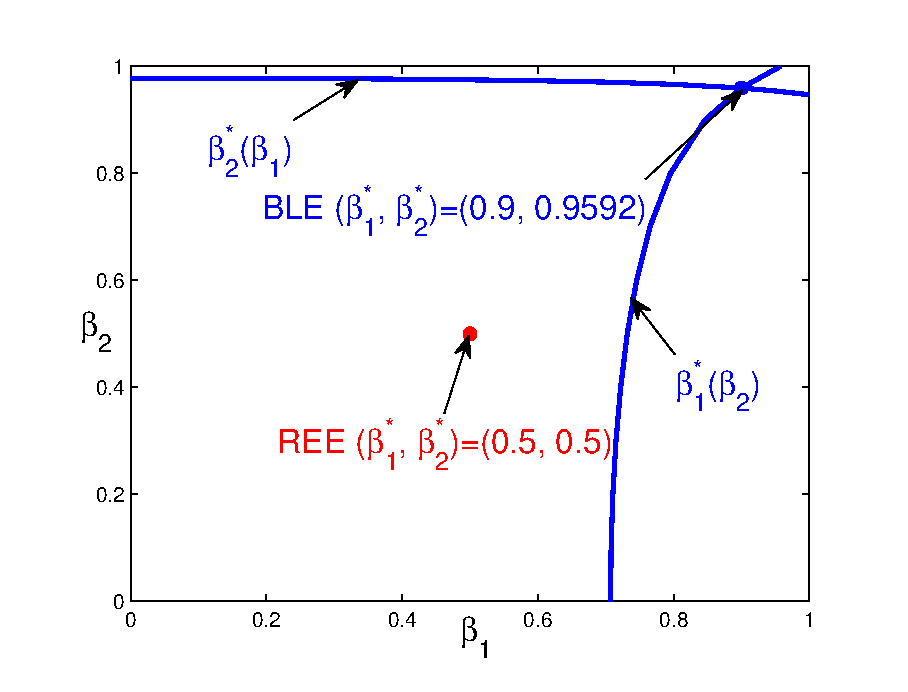
\includegraphics[width=4in]{ble_fig1.eps}
       % \subfigure[]
%        {\includegraphics[width=3in]{blew1.eps}}}
    \end{center}
   \caption{ \label{ble} A unique BLE $(\beta_1^*,\beta_2^*)=(0.9, 0.9592)$ obtained as the intersection point of the fixed point curves $\beta_2^*(\beta_1)$ and  $\beta_1^*(\beta_2)$. The BLE exhibits strong persistence amplification compared to REE (red dot, with $\rho=0.5$). Parameters are: $\lambda=0.99, \varphi=1, \gamma=0.04, \rho=0.5, \phi_\pi=1.5,\phi_y=0.5, \frac{\sigma_{\pi}}{\sigma_y}=0.5$.}
    \end{figure}




\begin{figure}
    \begin{center}
        \mbox{\subfigure[]
        {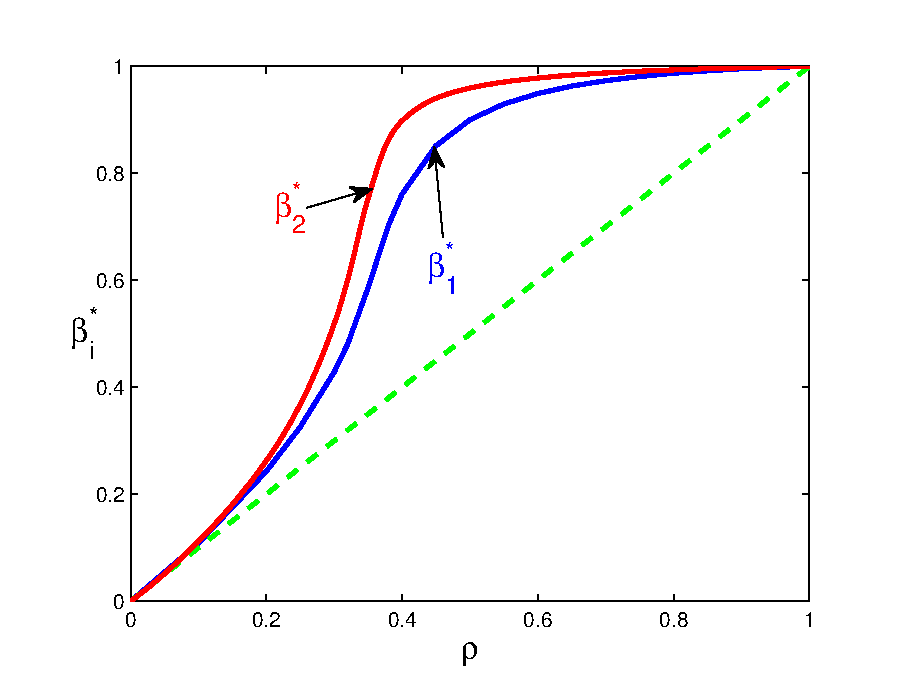
\includegraphics[width=3in]{blerhotrc.eps}}\quad
        \subfigure[]
         {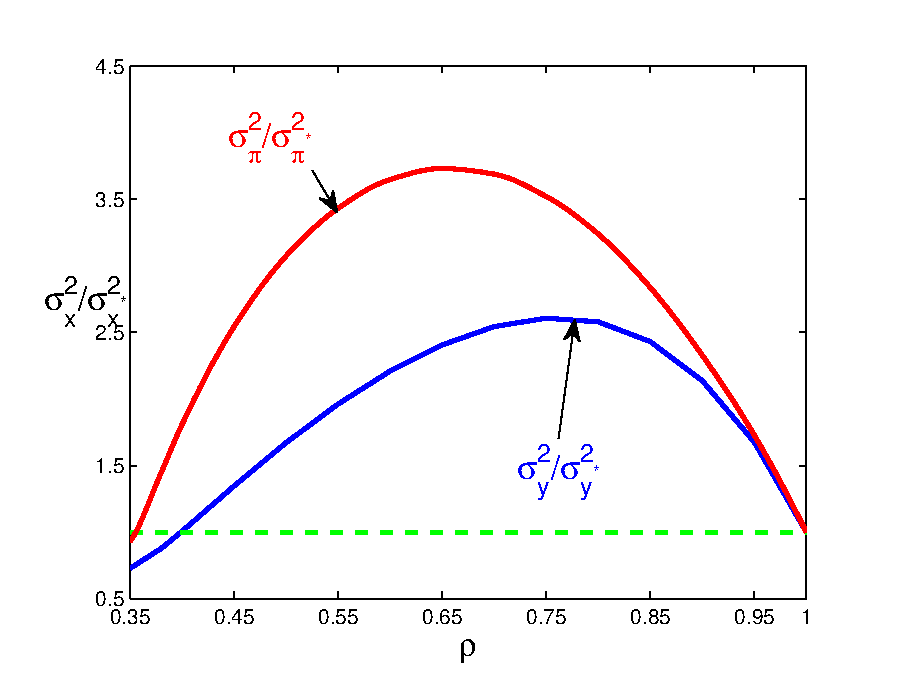
\includegraphics[width=3in]{varrhotrc.eps}}}
   \end{center}
   \caption{ \label{blerhotrc}
   BLE $(\beta^*_1, \beta^*_2)$ as a function of the persistence $\rho$ of the exogenous shocks. (a) $\beta^*_i (i=1,2)$ with respect to $\rho$; (b) the ratio of variances ($\sigma_y^2/\sigma_{y^*}^2$, $\sigma_\pi^2/\sigma_{\pi^*}^2$) of the BLE $(\beta^*_1, \beta^*_2)$ w.r.t. the REE. Parameters are: $\lambda=0.99, \varphi=1, \gamma=0.04, \phi_\pi=1.5,\phi_y=0.5, \frac{\sigma_{\pi}}{\sigma_y}=0.5$. }
\end{figure}



Figure~\ref{blerhotrc} illustrates how these results depend on the persistence $\rho$ of the exogenous shocks. The figure shows the BLE, i.e. the first-order autocorrelations $\beta_1^*$ of output gap and $\beta_2^*$ of inflation, as a function of the parameter $\rho$. This figure clearly shows the {\it persistence amplification} along BLE, with much higher ACF than under RE, for all values of $0< \rho <1$. Especially for $\rho\geq 0.5$ we have $\beta_1^*,\beta_2^* \geq 0.9$, implying that output gap and inflation have significantly higher persistence than the exogenous driving forces. Figure~\ref{blerhotrc} (right plot) also illustrates the {\it volatility amplification} under BLE compared to REE. For output gap the ratio of variances $\sigma_y^2/\sigma_{y^*}^2$ reaches a peak of about $2.5$ for $\rho\approx 0.75$, while for inflation the ratio of variances $\sigma_\pi^2/\sigma_{\pi^*}^2$ reaches its peak of about $3.5$ for $\rho\approx 0.65$. These results suggest that, given the same parameter values, the moments of inflation and output gap implied by BLE and REE are substantially different due to persistence and volatility amplification under BLE. Therefore if the model is estimated on the same dataset under BLE and REE, one might expect important differences in the resulting parameter estimates and the resulting shock propagation mechanism of the model. We explore this implication in the next section by estimating the model under BLE and REE based on U.S. data. 




\subsection{Estimation of The Baseline Model} 
\label{sec:estimation_ble}

\subsubsection*{Sample Period and Prior Distributions}

In this section, we compare the empirical fit of the 3-equation New Keynesian model under  REE, BLE and SAC-learning. We augment the Taylor rule with an i.i.d monetary policy shock and an interest rate smoothing parameter to allow the model to match the inertia of the historical interest rate: 
\begin{equation}
r_t = \rho_r r_{t-1} + (1-\rho_r) (\phi_{\pi}\pi_t +\phi_x y_t) +\epsilon_{r,t}.
\label{eqn:3_1}
\end{equation}

\noindent

We estimate the small-scale system of  (\ref{nkmodel}) and (\ref{eqn:3_1}) for the U.S economy over the period 1966:I-2016:IV using quarterly macroeconomic data. We also investigate whether our results are sensitive to structural breaks such as the large volatility reduction for most macroeconomic time series during the mid-80s, often referred to as the Great Moderation, or the near-zero level of nominal interest rates that followed the 2007-08 crisis period. 
%The U.S economy has experienced a large volatility reduction in most macroeconomic parameters in mid-80s, often referred to as the Great Moderation. Nevertheless we consider the entire sample period in this section: Inflation is highly persistent over the entire sample period, while its persistence is substantially reduced if we consider the post Great Moderation period. The highly persistent series allow us to illustrate the persistence amplification under the BLE estimation. Furthermore, empirical studies involving the U.S interest rate typically do not cover the post-2007 period due to concerns over the zero lower bound. Therefore, while we ignore the potential impact of the ZLB constraint in our main estimations, we show that the results are robust to different sample periods later on\footnote{Furthermore, recent studies show that, if there are any biases at all on the estimated parameters related to ignoring the ZLB, these are limited to steady-state and monetary policy related parameters, while the rigidity and structural shock parameters remain unaffected. See \citet{hirose2016parameter} and \citet{hirose2016zero} for more details.}.
We use the following measurement equations for output gap, inflation and interest rate\footnote{See Appendix \ref{app_data} for more details on the observable variables.} without measurement errors:
\begin{equation}
\begin{cases}
log(y_t^{obs})= \bar{\gamma}+y_t \\
log(\pi_t^{obs})=\bar{\pi} + \pi_t\\
log(r_t^{obs}) = \bar{r} + r_t, \\
\end{cases}
\label{eqn:3_2}
\end{equation}
\noindent
where we use the cycle component of HP-filtered quarterly output as our measure of output gap\footnote{As shown in the next section, our main results are not sensitive to the choice of output gap measure.} ${y_t^{obs}}$, while $ \pi_t^{obs} $ and $r_t^{obs} $ denote the quarterly historical inflation and interest rate series respectively. $\bar{\gamma}, \bar{\pi} $ and $ \bar{r}$ correspond to the historical mean levels of output gap, inflation and interest rate. The model is estimated using the same prior distributions under all three specifications, which guarantees that any differences that arise between the estimations is due to the difference in the expectation formation rule. The prior distributions are kept close to those commonly assumed in the literature: the risk aversion coefficient $\tau= \frac{1}{\varphi}$ is assigned a gamma distribution centered at 2 with a standard deviation of 0.5, covering values of approximately up to four. The slope of the Phillips curve $ \gamma$ is assigned a Beta distribution with mean $ 0.3$ and standard deviation $0.15$  which falls somewhere between the prior in An \& Schorfheide (2007) and Smets \& Wouters (2007), covering both flat and steep cases for the Phillips curve\footnote{In particular if we denote the nominal price stickiness as $\omega$, its relation with $\gamma$ is given as $\gamma=\frac{(1-\lambda \omega)(1-\omega)}{\omega}$ (Gali, 2008). Smets \& Wouters (2007) assume a prior for $\omega$ with mean $0.5$.}.  The policy response parameters for output gap and inflation are assigned beta distributions centered around $ 0.5$ and $ 1.5$, which are standard values associated with the Taylor Rule in the literature. The autocorrelation coefficients have a Beta distribution centered at 0.5, and the standard deviations for the shock processes are assumed to follow an Inverted Gamma distribution with a mean of 0.1 and standard deviation of 2, same as in Smets \& Wouters (2007). The priors for the steady-state inflation rate, output growth and interest rate are normal distributions centered at their pre-sample means of $0.47$, $-0.2$ and $0.72$ respectively, where the pre-sample period covers data from 1954:I to 1965:IV.  Finally, we fix the HH discount rate $\lambda$ at 0.99, which is a standard assumption in most empirical studies.\\


%\begin{table}

%\centering
%\caption{\small Prior Distributions for the Structural Parameters of the Small-Scale NKPC Model.}
%\label{table:table2}
%\vspace{5 mm}
%\begin{tabular}{l|l|l|l}

%Parameter & Dist. & Mean & St. Dev   \\
%\hline
%\hline
%$\eta_y$ & Inv Gamma & 0.10 & 2   \\
%$\eta_{\pi}$ & Inv Gamma & 0.10 & 2  \\
%$\eta_r$ & Inv Gamma & 0.10 & 2   \\
%$\bar{\pi}$ & Normal & 0.47 & 0.25  \\
%$\bar{y}$ & Normal & -0.2 & 0.25  \\
%$\bar{r}$ & Normal & 0.72 & 0.25 \\
%$\frac{1}{\psi}$ & Gamma & 2 & 0.50  \\
%$\gamma$ & Beta & 0.3 & 0.15   \\
%$\rho_y$ & Beta & 0.50 & 0.20   \\
%$\rho_{\pi}$ & Beta & 0.50 & 0.20  \\
%$\rho_r$ & Beta & 0.50 & 0.20  \\
%$\phi_y$ & Gamma & 0.50 & 0.25  \\
%$\phi_{\pi}$ & Gamma & 1.5 & 0.25  \\


%\end{tabular}
%\label{table1}
%\end{table}

\subsubsection*{Convergence Diagnostics}
Table \ref{table3} presents the posterior estimation results for the BLE, RE and SAC-learning models.\footnote{BLE and REE models are estimated using the Dynare toolbox (Adjemian et. al, 2011), while our own toolbox is used for the SAC-learning estimations since it requires an additional learning step in the filter recursions. The posterior distributions are constructed using the Metropolis-Hastings algorithm with 250000 draws, using the first 50000 as the burn-in sample. The step size for the scale parameter of the jumping distribution's covariance matrix is adjusted in both models to obtain a rejection rate of ~70\% in both models, which is in the commonly assumed {appropriate} range for the MH algorithm.} Before moving onto the estimation results, we first briefly discuss the convergence diagnostics of {BLE} and SAC-learning. Under BLE, initializing both $\beta_y$ and $\beta_{\pi}$\footnote{In this section we switch to the notation $\beta_y$ and $\beta_{\pi}$ instead of $\beta_1$ and $\beta_2$ to make the exposition more clear.} at fairly low values of 0.5 and using a convergence criterion $\epsilon=10^{-5}$, our estimation algorithm takes only 5 steps to converge\footnote{The results are robust to initial values of $\beta_y$ and $\beta_{\pi}$.}. The resulting BLE is $\boldsymbol (\beta_y^{*},\beta_{\pi}^{*})=(0.88,0.89)$ at the final step. This is fairly close to the sample-autocorrelation moments of the data over this period, which is $(0.87,0.89)$. The left panel of Figure \ref{nkm_convergence} shows the norm distances between two consecutive sets of $\pmb{\beta}^{(k)}$ and $\theta^{(k)}$ at each step $k$, both of which rapidly converge towards 0. The largest eigenvalue of the Jacobian matrix $DG(\pmb{\beta}^{(k)},\theta^{(k)})$ remains strictly inside the unit circle during the estimation, and stabilizes after the second step. The right panel of the same figure shows the convergence of Algorithm I towards $\pmb{ \beta}^{*} $ at the estimated posterior mode with randomized initial values, suggesting that the estimated equilibrium is the unique iteratively E-stable BLE. Similar results emerge when we examine the Monte Carlo simulations of the model under SAC-learning in Figure  \ref{nkm_sac_MC}: the left panel shows the histograms of $\beta_y$ and $\beta_{\pi}$ over 1000 simulations under decreasing gain learning, while the right panel shows the constant gain equivalent with a small gain value of $0.001$. It is readily seen that none of the distributions show signs of multiplicity of equilibria. To formally check this, we provide the approximate distributions of $\beta_y$ and $\beta_{\pi}$ by smoothing the histograms and applying Hartigan's Dip Test of Unimodality\footnote{Hartigan's Dip Test is based on checking for multimodality by using the maximum difference between the empirical distribution, and the theoretical unimodal distribution function that minimizes the maximum difference. The null hypothesis of the test is unimodality, see Hartigan \& Hartigan (1985) for more details.}. The dip test  does not reject the null hypothesis of unimodality, suggesting that there is no evidence of multiple {BLE} at the estimated structural parameter values based on the simulations. We also observe a small bias in the simulations for both cases, where the peak of the distributions slightly deviates from the underlying BLE denoted by the dotted line. These Monte Carlo  simulations  illustrate the advantage of SAC-learning over the standard recursive least squares learning approach: although the autocorrelation coefficients are fairly close to unity for both $y_t$ and $\pi_t$, the time series never becomes explosive in our simulations. This is due to the natural projection facility of SAC-learning, with autocorrelations always satisfying $-1 \leq \beta \leq 1$. This makes explosive time paths less likely as discussed in Section 2. 


Figure \ref{nkpc-sac-figure} shows the mean and persistence coefficients along with the filtered variables of inflation and output gap under the SAC-learning estimation. For this specification, following the recommendation in Galimberti \& Jacqueson (2017), we use a training-sample based initialization as follows: we use the unconditional moment of 0 for the intercept coefficients, and the diffuse moment 0 for the estimated variance of each variable $R_t$\footnote{The initial choice of first-order autocorrelations does not matter since $\beta_{1,t}=-\frac{1}{2}$ regardless of what $\beta_{0,t}$ is.}. We use a period of five years over 1961:I-1965:IV as the transient period for the belief coefficients, and compute the likelihood from 1966:I onwards. It is readily seen that the mean coefficients do not substantially deviate from the unconditional mean of 0 and the persistence coefficients indeed converge over the estimation sample, with final values of $\boldsymbol \beta^{*}=(0.86, 0.89)$: this is fairly close to the equilibrium resulting under the BLE estimation. 



\subsubsection*{Posterior Estimation Results}
\noindent
Next we move onto the discussion of our structural parameter estimates. Starting with a comparison of the BLE and REE results, we observe several important differences: both persistence parameters for the inflation and output shocks, $\rho_{\pi} $ and $\rho_y$, are substantially lower under BLE, namely with $0.31$ and $0.42$ respectively, while they are $0.88$ and $0.87$ under REE. This is a direct consequence of the difference in the expectation formation rule, and the estimation results confirm the persistence amplification property of a BLE. This backward-looking expectation rule endogenously generates additional inertia for inflation and output gap, which in turn leads to much smaller persistence in the exogenous shocks. The low autocorrelations in $u_{\pi}$ and $u_y$ under BLE immediately imply higher estimated standard deviations for the i.i.d shocks of these AR(1) processes at $0.29$ and $0.73$, while these are $0.04$ and $0.16$ under REE\footnote{ Note that for an AR(1) process $ x_t = \rho_x x_{t-1} + u_t,u_t\sim iid(0,\sigma_u)$, the unconditional variance is given by $var(x)=\frac{\sigma_u}{1-\rho_x^2}$. This implies, as $ \rho_x$ increases, $var(x)$ also increases.}. Since interest-rate is not forward-looking, this result does not extend to the interest-rate smoothing $\rho_r$, which is estimated at $0.85$ and $0.80$ under BLE and REE respectively, while the volatility of monetary policy shocks is the same at $0.29$ under both specifications. The steady-state parameters turn out fairly similar under both estimations, since they relate to sample means of the observable variables and are not affected by the expectation rule. The estimates of monetary policy parameters, $\phi_{\pi}$ and $\phi_y$ also turn out similar under both estimations, with $1.36$ and $0.48$ under BLE, and $1.39$ and $0.46$ under REE. Finally turning to the two structural parameters that determine the contemporaneous relation between the state variables, both the risk aversion coefficient $\frac{1}{\varphi}$ and the slope of the NKPC $\gamma$ turn out fairly different: these are estimated at $3.02$ and $0.035$ under BLE, while they are $4.27$ and $0.007$ under REE respectively. These differences arise due to altered cross-restrictions under learning:  the additional inertia that we introduce under learning comes at the cost of a weaker contemporaneous relation between the state variables and shocks. While the state variables are only related to the shocks through $\frac{1}{\varphi}$ and $\gamma$ under BLE, they are also indirecly related through expectations under REE. As a result, the risk aversion coefficient turns out lower under learning, implying a larger direct impact from the ex-ante risk premium on output gap under BLE. Similarly, $\gamma$ turns out higher under BLE, implying a stronger direct effect from output gap on inflation. %The identity $\gamma=\frac{(1-\lambda \omega)(1-\omega)}{\omega}$ in turn implies the estimated nominal price stickiness $\omega$ is lower under BLE with around 0.83, while it is around 0.92 under REE.
It is also interesting to note that confidence intervals for $\gamma$ are almost mutually exclusive under these two specifications, with a lower bound of $0.015$ under BLE and an upper bound of $0.017$ under REE\footnote{As noted in the previous section, the first-order coefficients are computed based on the posterior mode values. Therefore for completeness, the discussion and comparison of these results (both in this section and in the upcoming ones) are based on the posterior mode. It is worth noting that, given the small differences across the posterior means and modes, a similar discussion can be easily extended to the posterior mean.}. 
\noindent





\begin{sidewaystable}
\centering

\label{table3}
\vspace{2 mm}
%\resizebox{18 cm}{!}{
\begin{tabular}{l|lll|llll||llll||llll}
& & & &      & REE &      &    &  & BLE &   &  &  & SAC &      &       \\
 \hline
 \hline
& & & Laplace      &      & -348 &  & &  &  -337  &       &  &  & -341 &      &       \\
& & & MHM          &      & -348 & &  &  &  -337   &       &  &    & -341 &      &       \\
\hline
\hline
& & & Bayes Factor          &      & 1 & &  &  & 4.78    &       &  &    & 3.04 &      &       \\
\hline
\hline
& Prior& &           &   Post.   &  & &  & Post. &     &       &  &  Post.  &  &      &       \\
\hline
\hline
Para. & Dist.&Mean&St. Dev    & Mode & Mean    & 5 \% & 95 \% &  Mode & Mean    & 5 \% & 95 \%                     & Mode       & Mean    & 5 \% & 95 \% \\

\hline
\hline
 $\sigma_y$  & Inv. Gamma &0.1&2& 	0.16     & 0.17    & 0.12 & 0.22  		&	0.73 & 0.74    & 0.68 & 0.8                   &    0.75 & 0.76 & 0.68 & 0.83   \\
 $\sigma_{\pi}$ & Inv. Gamma &0.1&2&	0.04     & 0.04    & 0.03 & 0.05 		& 	 0.29 & 0.3     & 0.27 & 0.32                 &  0.3 & 0.3 & 0.28 & 0.33 \\
 $\sigma_r$  & Inv. Gamma &0.1&2&		0.29     & 0.3     & 0.28 & 0.33 		&	 0.29 & 0.29     & 0.27 & 0.32                &   0.29 & 0.29 & 0.27 & 0.32    \\
 $\bar{y}$  &Normal&-0.2&0.25&		-0.15    & -0.49    & 0.18  			&	 -0.12 & -0.12    & -0.4    & 0.17&   -0.17   & -0.21 	& -0.19 & -0.6 & 0.22\\
 $\bar{\pi}$ &Normal&0.47&0.25&		0.7     & 0.71    & 0.53 & 0.9 			&	 0.79 & 0.79    & 0.67 & 0.91              	  &    0.41 & 0.45 & 0.18 & 0.75        \\
 $\bar{r}$  &Normal&0.72&0.25&		0.98     & 0.98    & 0.71 & 1.26  		& 	 1.1 & 1.09    & 0.85 & 1.32                  &    0.65 & 0.7 & 0.33 & 1.06      \\
 $\gamma$  &Beta&0.3&0.15&			0.007     & 0.01    & 0.002  & 0.017    &	 0.035 & 0.037    & 0.015 & 0.065             &  0.048 & 0.048 & 0.019 & 0.08 \\
 $\frac{1}{\varphi}$  &Gamma&2 & 0.5&	4.27     & 4.35   & 3.35 & 5.37 		& 	 3.02 & 3.15    & 2.33 & 3.98       		  &   2.86 & 2.98 & 2.04 & 3.94   \\
 $\phi_{\pi}$ &Gamma&1.5&0.25&		1.38     & 1.4   & 1.16 & 1.65   		& 	 1.36 & 1.38   & 1.1 & 1.67  				  &   1.32 & 1.35 & 1.03 & 1.69     \\
 $\phi_y$  &Gamma&0.5&0.25&			0.48     & 0.51    & 0.34 & 0.67 		&	 0.49 & 0.52    & 0.31 & 0.73                 &     0.48 & 0.51 & 0.29 & 0.76  \\
 $\rho_y$  &Beta&0.5&0.2&			0.87     & 0.86    & 0.83 & 0.92 		& 	 0.43 & 0.43    & 0.32 & 0.53                 &     0.57 & 0.57 & 0.46 & 0.68 \\
 $\rho_{\pi}$ &Beta&0.5&0.2&		0.88     & 0.87    & 0.82 & 0.91  		&	 0.32 & 0.32    & 0.22 & 0.43                 &    0.25 & 0.26 & 0.14 & 0.38           \\
 $\rho_r$     &Beta&0.5&0.2& 		0.8     & 0.8     & 0.76 & 0.84 		& 	0.85 & 0.86    & 0.82 & 0.91                  &    0.85 & 0.86 & 0.81 & 0.81    \\
 $\beta_y^{*}$ & & & & 		-     &  -    & - & 	-	& 	0.88 &  -  & - &     -              &    0.86 & - & - &   -   \\
 $\beta_{\pi}^{*}$ & & & & 		-    &   -   & - & 	-	& 	0.89 &  -  & - &    -               &    0.88 & - & - & -     \\
\end{tabular}
%}

\caption{\small Posterior results under REE, BLE and SAC-learning over the estimation period 1966:I-2016:IV. Lapl. refers to the Laplace approximation of likelihood based on the posterior mode, while MHM refers to the Modified Harmonic Mean estimate of likelihood based on the posterior distribution. }
\label{table2}
\end{sidewaystable}





\begin{figure}
    \centering
 
             \mbox{\subfigure[Convergence towards $\pmb{ \beta^{*}}$]{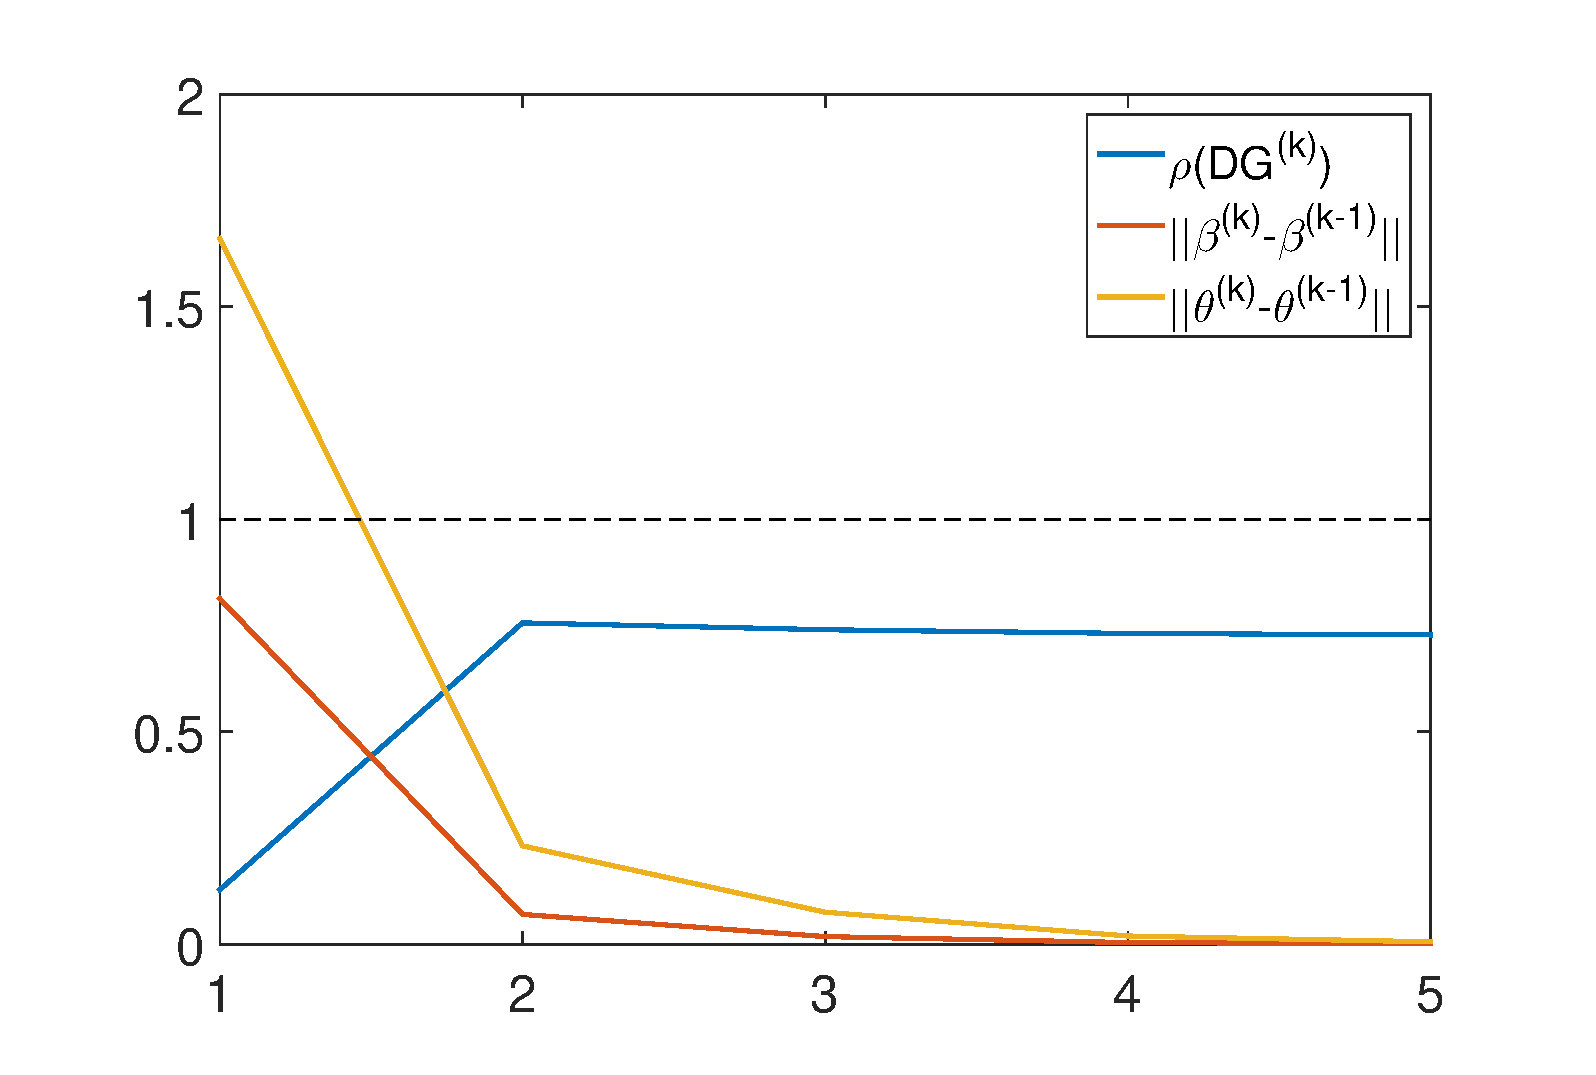
\includegraphics[scale=0.3]{diagnosticsNKPC.eps} }
       \subfigure[Iterative E-stability of the unique $\boldsymbol \beta^{*}$]{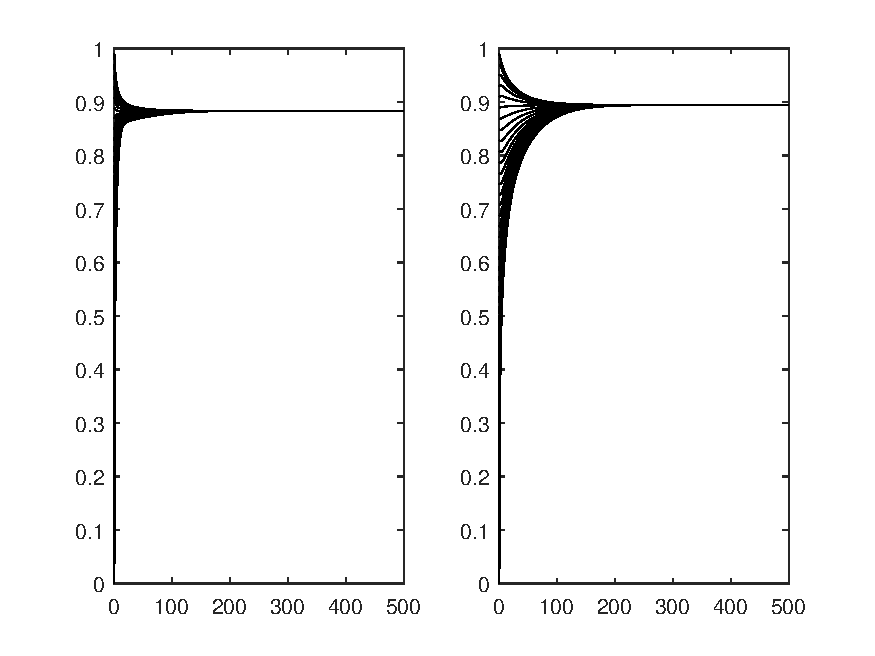
\includegraphics[scale=0.5]{NKPC_estimated_fixedPoint_iter.pdf}}}\\
 
      \caption{The estimated BLE is $(\beta_y^*,\beta_{\pi}^*)=(0.88, 0.89)$. The left panel shows the largest eigenvalue, and the norm distances between consecutive values of $\pmb{\beta^{(k)}}$, as well as $\theta^{(k)}$ across iterations. The second panel shows convergence towards the unique (iteratively) E-stable BLE with randomized initial values.}     
      \label{nkm_convergence}
\end{figure}
    

    \begin{figure}
    \mbox{\subfigure[$\beta_y^{*}$ and $\beta_{\pi}^{*}$ under constant gain learning.]{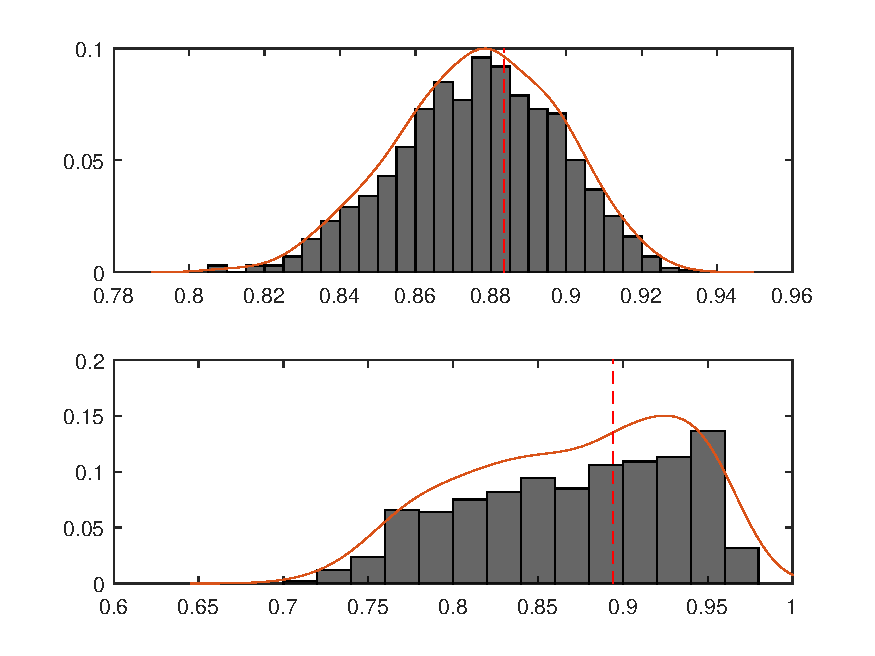
\includegraphics[scale=0.55]{NKPC_MC_cgl.pdf}}
 \subfigure[$\beta_y^{*}$ and $\beta_{\pi}^{*}$ under decreasing gain learning.]{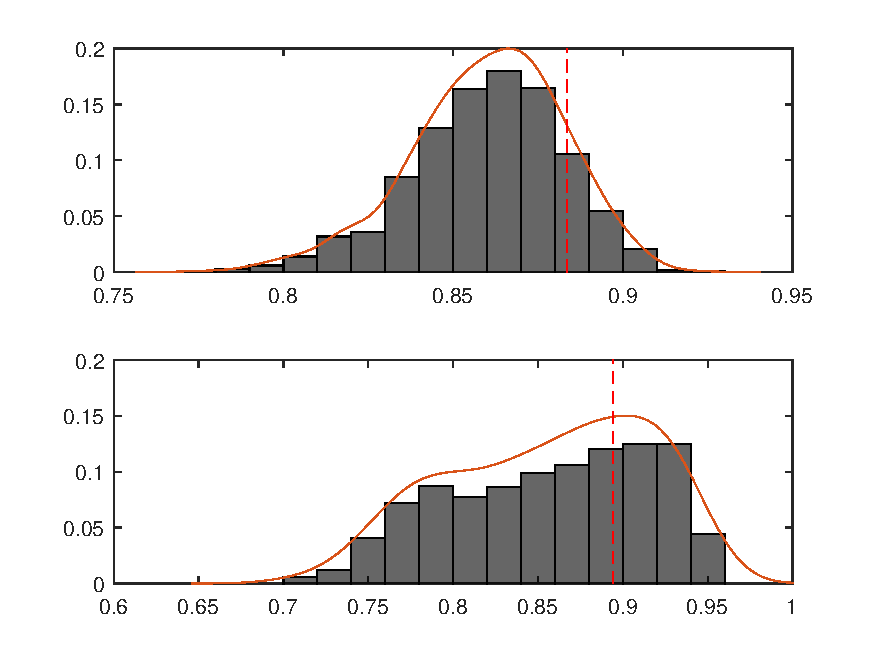
\includegraphics[scale=0.55]{NKPC_MC_dgl.pdf}}}\\

  \caption{ Monte Carlo Simulations: frequency distributions and unimodality test for $\beta_y$ and $\beta_{\pi}$ resulting from 1000 simulations. Hartigan's unimodality test p-values are $ 0.98$ and $0.94$ for $\beta_y$ and $\beta_{\pi}$  under constant gain simulations, and $ 0.99$ and $0.99$ for the decreasing gain simulations. Hence the null hypothesis of unimodality is not rejected for any of the distributions.
   }
  \label{nkm_sac_MC}
\end{figure}

\begin{figure}
    \centering

    \vspace{3 mm}
    \mbox{\subfigure[Filtered Variables and mean parameters]{
    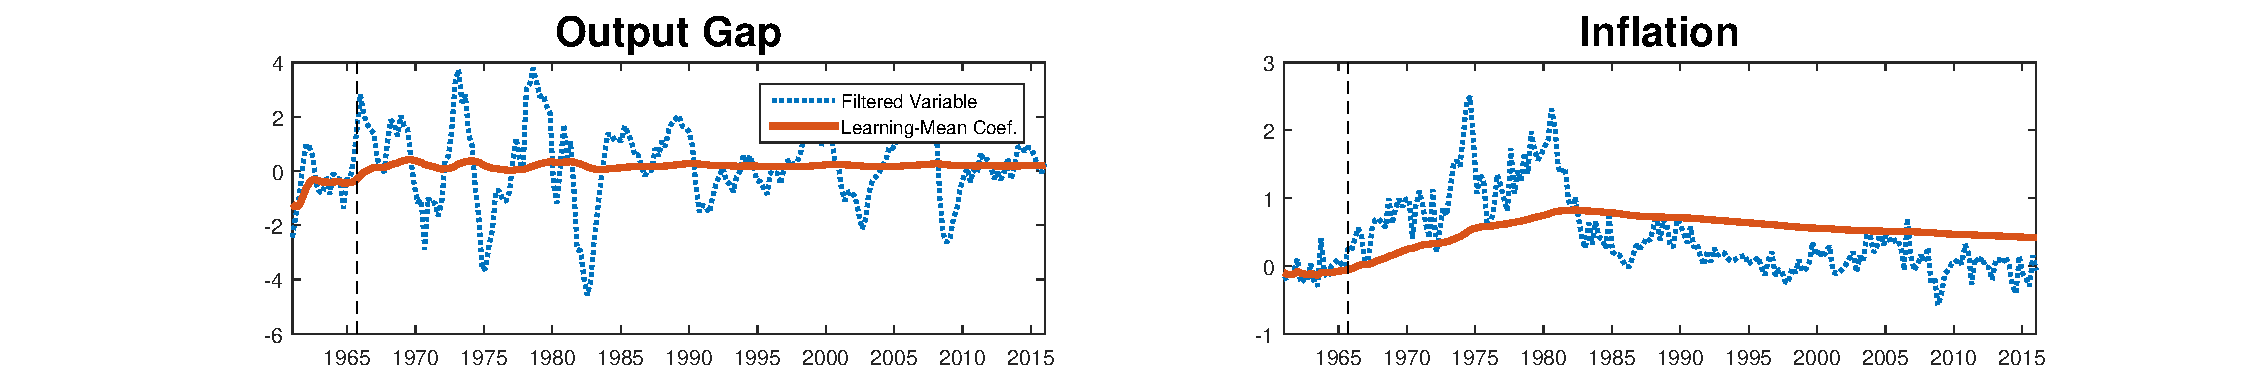
\includegraphics[scale=0.5]{NKPC_alphas.pdf}}}\\
     \mbox{\subfigure[Persistence parameters]{
    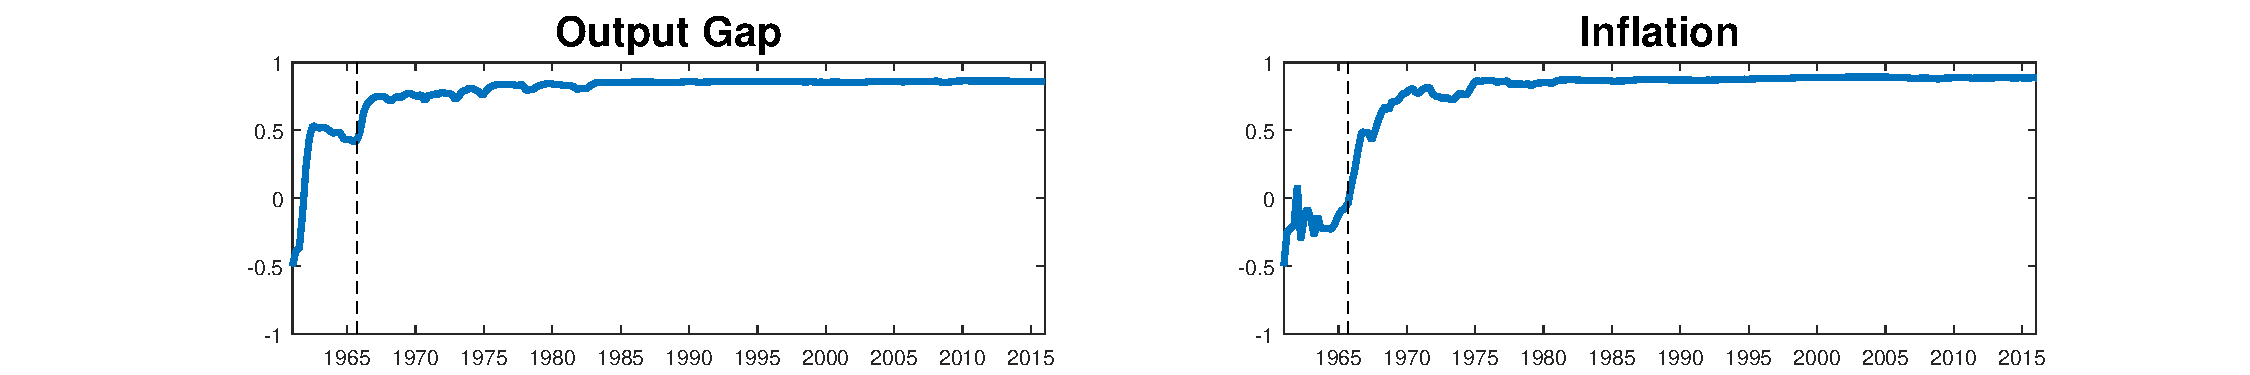
\includegraphics[scale=0.5]{NKPC_betas.pdf}}}\\
    
        \caption{Filtered variables and learning parameters over the estimation sample under SAC-learning, where Kalman filter output is used to update the belief coefficients. Converged values of first-order autocorrelations are $0.86$ and $0.89$ for output gap and inflation respectively.}
    \label{nkpc-sac-figure}
\end{figure}

Overall, our results suggest important differences in the estimated parameters and the propagation of shocks under BLE. These changes lead to a substantial improvement in the empirical fit, evident from the (log marginal) likelihood of $-337$ under BLE compared with $-348$ under REE, which yields a Bayes' Factor $4.78$ in favour of BLE\footnote{Based on Jeffrey's Guidelines (Greenberg, 2012), if the Bayes' Factor is in favour of a model is larger than 2, then this provides \textit{decisive support} for the model under consideration.}. Comparing the results to SAC-learning, it is readily seen that there are no substantial differences with the BLE specification. Relative to the REE estimations, the exogenous shocks have lower persistence and larger standard deviations, the risk aversion coefficient is lower, Phillips curve slope is higher and monetary policy coefficients are similar. The only difference with the BLE model arises in the steady-state values of inflation and interest-rate, which turn out lower under the SAC-learning estimation. This difference arises since the learning coefficients are time-varying under real-time SAC-learning and Figure \ref{nkpc-sac-figure} suggests that they are slightly above zero on average, which drives down the estimates of the steady-state parameters\footnote{Shutting off the learning dynamics about mean coefficients and letting the agents learn only about the first-order autocorrelations indeed yields steady-state values similar to BLE.}. Other than these small differences, all parameter estimates are fairly close under BLE and SAC-learning, with implied HPD-intervals well within the range of each other. The likelihood turns out to be $-341$ under SAC-learning, which is still better than the fit of REE, with a Bayes' Factor of 3.08 in favour of SAC-learning, but worse than BLE, with a Bayes' Factor of 1.7 in favour of BLE\footnote{Based on Jeffrey's Guidelines, this provides \textit{very strong} evidence in favour of BLE.}. This result suggests that transitory dynamics and the resulting time-variation in the learning parameters do not improve the model fit in our decreasing-gain learning setup. Overall, these results also allow us to illustrate the advantage of using Algorithm II to estimate a BLE: the estimation under SAC-learning requires a relatively large burn-in sample for the convergence of first-order autocorrelation coefficients. This might become an issue if the researcher does not have a sufficiently long dataset, as is typical in most quarterly macroeconomic time series. Furthermore, as we have already seen in Figure \ref{nkm_sac_MC}, the simulations under learning have a relatively large Monte-Carlo variance. In other words, while the simulations converge to the underlying BLE on average, there might be relatively large deviations from the underlying fixed-point for any given simulation. Hence what comes out of the estimation in a real-time learning setup is similar to a single simulation of the model under learning, which in general may not accurately reflect the underlying fixed-point. In the following, we check whether these results are robust to different measures of output gap and different subsamples for the BLE and REE specifications.


%\subsection{Impulse Responses}






%\begin{figure}

%\textbf{One standard deviation shocks (at the estimated value) on inflation and output. Left panel is BLE, right panel is REE. The grey areas depich the 90 \% confidence bands.}\\

%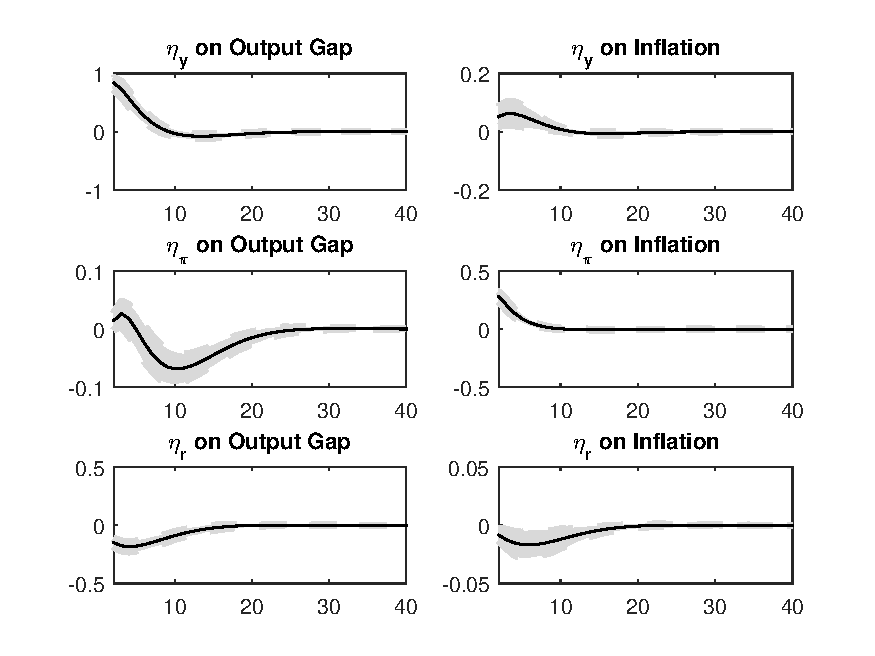
\includegraphics[scale=0.6]{nkpc_ble_irfs.pdf}
%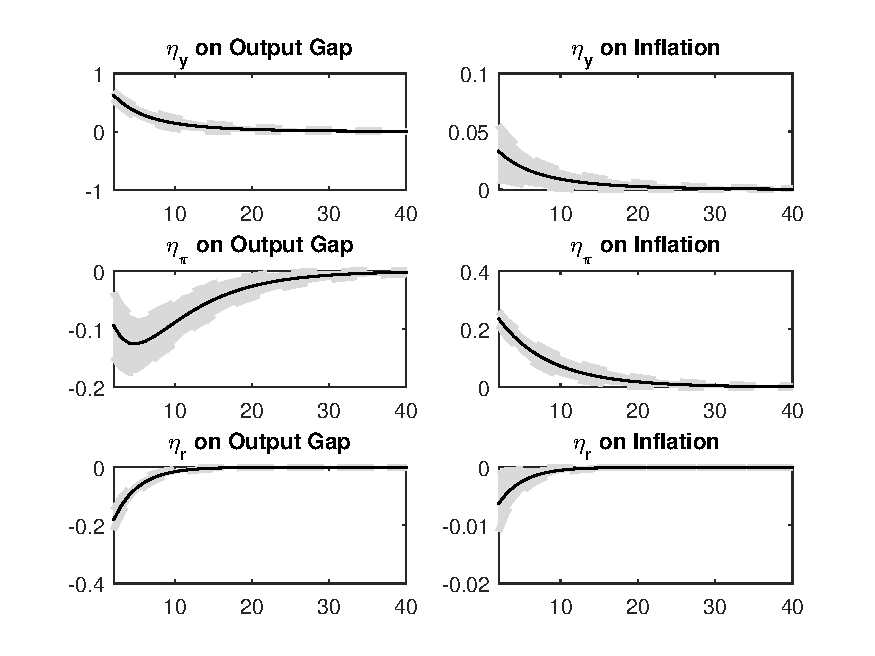
\includegraphics[scale=0.6]{NKPC_ree_irfs.pdf}\\

%\textbf{Comparison of responses under BLE and REE, the shocks are scaled to one under both specifications. }
%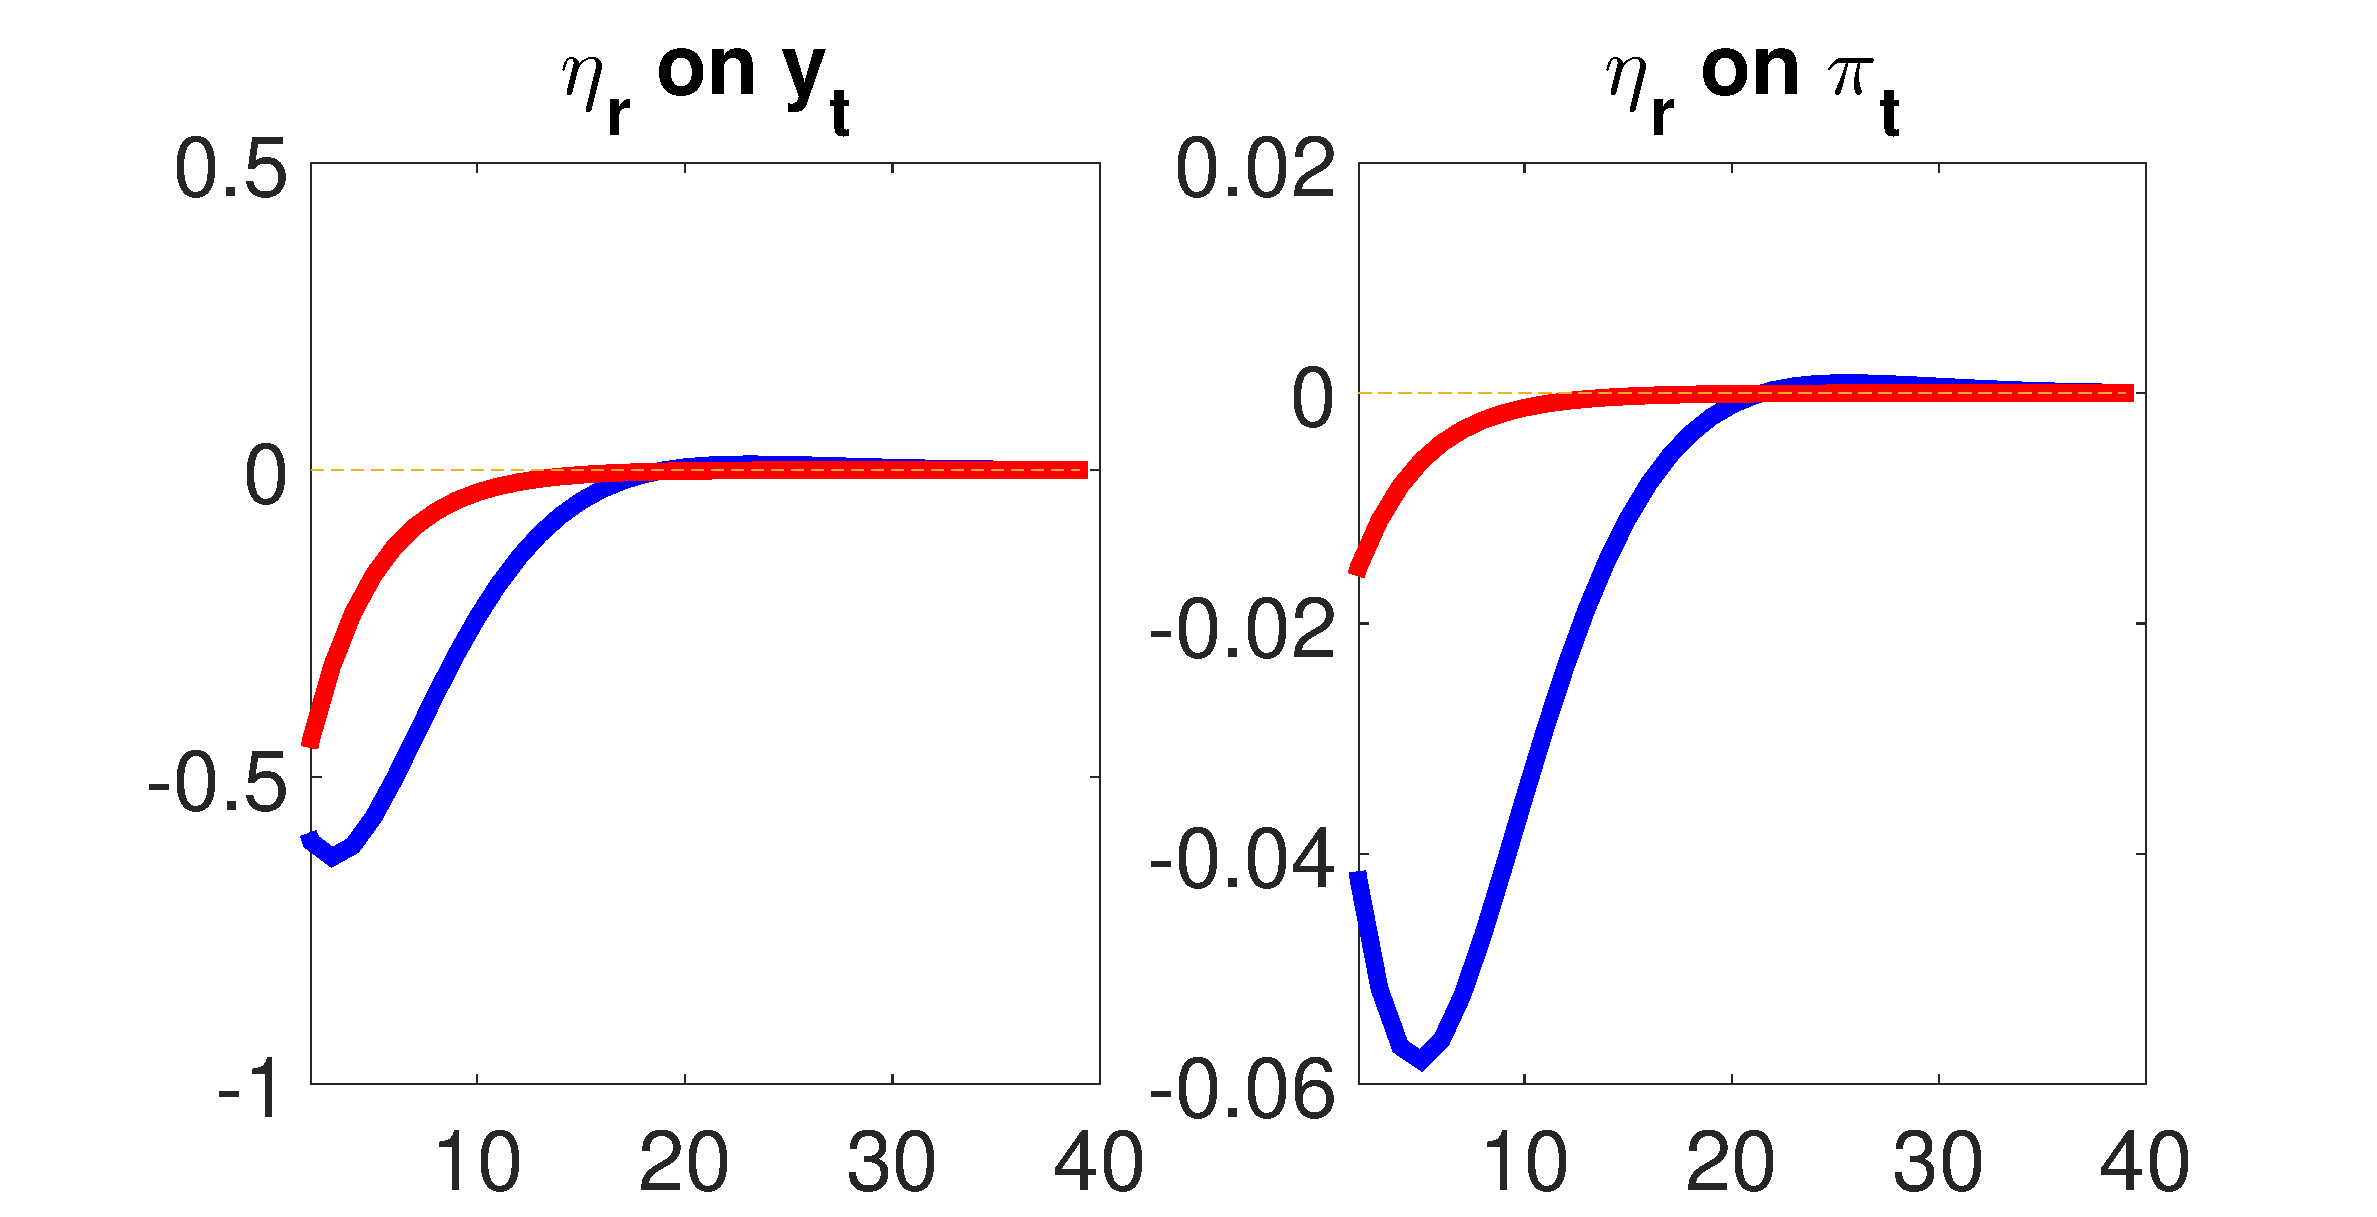
\includegraphics[]{nkpc_irfs_comparison.pdf}
%\end{figure}




\subsubsection*{Subsample Estimations}

We first chek whether our main results hold across different sample periods. To this end, we consider three periods: 1966:I-1979:II, the period before Great Moderation; 1966:I-2008:IV, the period before Great Recession and the zero lower bound episode; and 1984:I-2008:IV, the Great Moderation period. 

\noindent

Table \ref{nkm_subsample} reports the posterior mode and the corresponding Laplace approximation for all periods under BLE and REE. It is readily seen that the difference between parameter estimates are preserved across all three periods: BLE is characterized by lower persistence but larger standard deviation estimates in shocks, a steeper Phillips curve characterized by larger $\gamma$, and a smaller risk aversion coefficient. The estimation under BLE provides a better model fit under all three subsamples, with Bayes' Factors of $1.67$, $3.93$ and $2.44$ in favor of the BLE model. 




\begin{table}[!htbp]
\begin{tabular}{l||ll||ll||ll}
Period & 66:I-79:II &  & 66:I-08:IV & & 84:I-08:IV \\
\hline
\hline
 & BLE & REE & BLE & REE & BLE & REE\\
Laplace & -118.63 & -122.47 & -313.16 & -322.10 & -34.32 & -39.93 \\
\hline
Bayes Factor & 1.67 &  & 3.93 &  & 2.44 & \\
\hline
\hline
Parameter & Mode &  &Mode  &   & Mode \\
\hline
\hline
$\eta_y$ &    0.94 & 0.24 &     0.76 & 0.17 &   0.53 & 0.09\\
$\eta_{\pi}$ & 0.38 & 0.06 & 0.3 & 0.04 &       0.18 & 0.08\\
$\eta_r$     & 0.20 & 0.20 & 0.31 & 0.32 &      0.15 & 0.15\\
$\bar{y}$ & -0.22 & -0.14 &   -0.09 & -0.14 &    0.05 & -0.14\\
$\bar{\pi}$ & 0.93 & 0.75 &     0.84 & 0.71 &   0.61 & 0.58 \\
$\bar{r}$ & 1.03 & 0.86 &    1.25 & 1.08 &      1.14 & 0.97\\
$\gamma$ & 0.054 & 0.01 &     0.033 & 0.006 &   0.046 & 0.007\\
$\frac{1}{\psi}$ & 2.44 &   2.77 & 4.03 & 3.78 & 2.82 & 3.15\\
$\phi_{\pi}$ & 1.03 & 1.07 & 1.29 & 1.31 &      1.55 & 1.57\\
$\phi_y$ & 0.39 & 0.36 &     0.45 & 0.42 &      0.48 & 0.54\\
$\rho_y$ & 0.5 & 0.87 &     0.42 & 0.88 &       0.44 & 0.94\\
$\rho_{\pi}$ & 0.31 & 0.85 & 0.32 & 0.87 &      0.24 & 0.55\\
$\rho_r$ & 0.72 & 0.68 &     0.83 & 0.77 &      0.9 & 0.85\\
\end{tabular}
\caption{Comparison of the sub-sample estimations under BLE and REE.}
\label{nkm_subsample}
\end{table} 
%\afterpage{\clearpage}


\subsubsection*{Alternative Definitions of Output Gap}

Next we check whether our results are sensitive to which measure of output gap is considered by using two alternative definitions: output gap based on de-trended output, 
%\footnote{De-trending here is based on a $4^{th}$ order polynomial, which yields the best fit over our main sample.} 
and output gap based on CBO's measure of potential output. The estimations over our main sample are reported in Table \ref{nkm_alt_gap}, which yield the same conclusions as before:  BLE is characterized by lower persistence but larger standard deviation estimates in shocks, a steeper Phillips curve characterized by larger $\gamma$, and a smaller risk aversion coefficient. The likelihood is also better under BLE for both definitions, with Bayes' Factors of $11.49$ and $10.41$ respectively. As a final check, we compare the likelihoods across the three sub-samples with the alternative measures of output gap, which is reported in Table \ref{nkm_alt_subs}: it is readily seen that the likelihood under BLE is better for both measures under all sub-samples, although the difference for the Great Moderation period 1985-I:2008:IV is much smaller. These results are also consistent with our previous findings. \\




\begin{table}[!htbp]
\centering


\begin{tabular}{l||ll||ll}
 &     BLE det. &   REE det.   & BLE CBO.   & REE CBO.\\
 Laplace&      -360.96   & -387.42   & -342.9  & -366.88 \\
 \hline
 Bayes Factor &       11.49   &    & 10.41  &  \\
\hline
\hline
&        Post.  &  & Post. & \\
\hline
 Parameter & Mode &   Mode & Mode & Mode\\
$\eta_y$   &      0.78 &   0.08 &   0.74   & 0.11\\
$\eta_{\pi}$ &  0.3 &   0.04 &   0.29 &   0.04 \\
$\eta_r$ &     0.3   & 0.31   & 0.29   & 0.3 \\
$\bar{y}$  &     -0.13 &   -0.19   & -0.54 &   -0.42\\
$\bar{\pi}$    &  0.79 &   0.66 &   0.81 &   0.59 \\
$\bar{r}$ &      1.09 &   0.92 &   1.15 &   1.05 \\
$\gamma$  &     0.017 &  0.004 &   0.024 &   0.006\\
$\frac{1}{\psi}$  &       2.92 &   4.86   & 2.65 &   4.57 \\
$\phi_{\pi}$  & 1.44 &   1.45 &   1.41 &   1.43 \\
$\phi_y$  &     0.22 &   0.16 &   0.36 &   0.27 \\
$\rho_y$ &      0.42 &   0.88 &   0.42 &   0.89 \\
$\rho_{\pi}$  &  0.31 &   0.94 &   0.31 &   0.92 \\
$\rho_r$ &      0.88 &   0.79 &   0.88 &   0.8 
\end{tabular}
\caption{Alternative estimations of the 3-equation NKPC model: we compare the results under BLE and REE with two alternative specifications of output gap. In the first case output gap is defined as the deviation of output from a quadratic trend, while in the latter we take the output gap based on CBO's measure of potential output.  }
\label{nkm_alt_gap}
\end{table}

\begin{table}[!htbp]
\centering

\begin{tabular}{l||ll||ll||ll}
& 66:I-79:II & & 66:I-08:IV  & & 84:I-08:IV & \\
\hline
\hline

& BLE & REE & BLE & REE & BLE & REE  \\
\hline
\hline

CBO's estimate & -126.07 & -127.6 & -321.9 & -344.4 & -36.7 & -46.9\\
\hline
Bayes Factor & 0.66 &   & 9.77 &   & 4.43 &  \\
\hline
\hline
Detrended output & -129.9 & -133.1 & -333.1 & -353.2 & -48.4 & -66.9\\
\hline
Bayes Factor & 1.39 &   & 8.73 &   & 8.03 &  \\
\end{tabular}
\caption{Sub-sample estimations with alternative definitions of output gap. } 
\label{nkm_alt_subs}
\end{table}
%\afterpage{\clearpage}


\FloatBarrier

%\section{Results under Real-Time SAC-Learning}
\label{sec:estimation_dgl}
Our results in the previous section highlight that a BLE estimated under Algorithm II provides a better fit than the REE model. As an alternative to this algorithm, and a final robustness check, we consider the estimation of the same model under real-time SAC-learning. As we noted in Section \ref{sec:iterative_ble}, an iteratively E-stable equilibrium that results under Algorithm II is also E-stable, and hence it is also learnable under SAC-learning. Therefore, an alternative and indirect approach to estimate the underlying BLE is to let the agents learn in real-time over the estimation sample. Since the model is conditionally linear for a given set of belief coefficients, one can use the standard Kalman filter recursions to iterate the model forward. Then the beliefs are updated using the Kalman filter output. This is the standard approach in estimating adaptive learning models; see e.g Slobodyan \& Wouters (2012) and Milani (2005) for more details. While real-time learning estimations typically involve a constant-gain algorithm, we use our decreasing-gain version here in order to let the beliefs converge to the underlying BLE. \\
\noindent






Figure \ref{nkpc-sac-figure} shows the learning parameters for the mean and persistence along with the Kalman filter output. The learning parameters are initialized as follows: We use the unconditional moment of 0 for the intercept coefficients $\boldsymbol alpha_t$, and the diffuse moment 0 for the estimated variance of each variable $R_t$\footnote{The initial choice of first-order autocorrelations does not matter since $\beta_{1,t}=-\frac{1}{2}$ regardless of what $\beta_{0,t} is$.}. We use a period of five years over 1961:I-1965:IV as the transient period for the belief coefficients, and use the same sample period of 1966:I-2016:IV as in Section \ref{sec:estimation_ble} to estimate the model. \\
Table \ref{nkpc_sac} and Figure \ref{nkpc-sac-figure} report our estimation results: the first thing we notice is that, the learning parameters for persistence indeed converge, and their equilibrium values are fairly close to what we found in \ref{sec:estimation_ble} with $\boldsymbol \beta^{*}=(0.86, 0.89)$. This difference is due to small differences in the parameter estimates under BLE and SAC-learning estimations. While the learning parameter for output gap mean always remains close to zero, the inflation parameter is off-the equilibrium during the entire period and has not yet converged to zero at the end of the estimation sample. \\
\noindent
Next turning to the parameter estimates, a noticeable difference compared with BLE estimation arises in the steady-state values of inflation and interest-rate, which turn out to be lower in this case. This difference is expected since the learning coefficients for the mean are well above zero on average in this case, which drives down the estimates of the steady-state parameters\footnote{Shutting off the learning dynamics about mean parameters indeed yields steady-state values similar to BLE.}. Another difference arises in the first-order autocorrelation of the output gap shock, which turns higher under SAC-learning with a mode of $0.57$, compared with $0.42$ under BLE. Other than these small differences, all parameter estimates are fairly close under SAC-learning and BLE. The likelihood turns out to be $-341$, which is still better than the fit of REE and almost identical to that of BLE. This result suggests that transitory dynamics or the time-variation in the learning parameters do not improve the model fit in this decreasing gain learning context. 
This result suggests the transitory dynamics or the time-variation in the learning parameters do not improve the model fit in a decreasing gain learning context. Overall, these results also allow us to illustrate the advantage of using Algorithm II to estimate a BLE: The estimation under real-time learning requires a relatively large burn-in sample for the convergence of first-order autocorrelation coefficients, which might become an issue since macroeconomic time series are typically not very long. Furthermore, as we have already seen in the previous sections, the simulations under learning have a relatively large Monte-Carlo variance. In other words, while the simulations converge to the underlying BLE on average, there might be relatively large deviations from the underlying fixed-point for any given simulation. Hence what comes out of the estimation in a real-time learning setup may not always accurately reflect the underlying fixed-point. While these issues evidently do not arise in our estimation of the standard 3-equation model, they are more likely to be pronounced in the estimation of a medium-scale model such as Smets-Wouters (2007), in which case using the fixed-point approach becomes more advantageous. \\ \\
%\section{Optimal Monetary Policy}
\label{sec:MonPol}

Our results so far illustrate that, when BLE and REE are examined under the same set of calibrated parameter values, BLE are characterized by persistence and volatility amplification, with much higher persistence and variance in output gap and inflation compared with REE. As a consequence, there are substantial differences in the estimated parameters and propagation structure when the 3-equation model is evaluated under BLE and REE. This leaves an important question for the optimal Taylor-rule parameters at the BLE. As shown in Boehm and House (2014), at the REE when the output gap and
inflation are observed without error, it is typically optimal to respond infinitely strongly to observed deviation from the central bank's targets, while with measurement error the optimal Taylor rule coefficients are finite.
How do the optimal values of Taylor rule parameters differ between the BLE and REE? In this section we try to answer this question by considering optimal monetary policy under both the calibrated and estimated parameter values. 

Similar to Boehm and House (2014), Evans and Honkapohja (2003) and Woodford (2003), we assume that the central bank wishes to minimize an expected discounted sum of weighted squared inflation and output gap
\begin{equation}
(1-\vartheta)E\Big[\Sigma_{t=0}^\infty \vartheta^t[\omega\pi_t^2+(1-\omega)y_t^2] \Big]=\omega\sigma_\pi^2+(1-\omega)\sigma_y^2,\label{varobj}
\end{equation}
where $\omega$ is the relative weight that the central bank places on inflation. From the equations (\ref{varyapp}) and (\ref{varpiapp}) in Appendix \ref{acfnkc},
\begin{eqnarray}
\sigma_y^2&=&\frac{\widetilde{g}_1}{(1+\gamma\varphi\phi_\pi+\varphi\phi_y)^2(1-\rho^2)(1-\rho\lambda_1)(1-\rho\lambda_2)(1-\lambda_1^2)(1-\lambda_2^2)(1-\lambda_1\lambda_2)}, \label{varyc}\\
\sigma_\pi^2&=&\frac{\widetilde{g}_2}{(1+\gamma\varphi\phi_\pi+\varphi\phi_y)^2(1-\rho^2)(1-\rho\lambda_1)(1-\rho\lambda_2)(1-\lambda_1^2)(1-\lambda_2^2)(1-\lambda_1\lambda_2)}, \label{varpic}
\end{eqnarray}
where $\widetilde{g}_1$, $\widetilde{g}_2$, $\lambda_1$ and $\lambda_2$ are given by the equations (\ref{gyvar}), (\ref{gpivar}), (\ref{lambdatr}) and (\ref{lambdade}). In the following we study the optimal values  $(\phi_y^*, \phi_\pi^*)$ that minimize the central bank's loss function (\ref{varobj}) at the BLE   ($\beta_1^*, \beta_2^*$).

\begin{figure}
    \begin{center}
     \includegraphics[width=3.2in]{optpolicy09.eps}
     \end{center}
   \caption{\label{opt09} Optimal policies at the BLE and at the REE. Parameters are: $\lambda=0.99, \varphi=1, \gamma=0.04, \rho=0.5, \frac{\sigma_2}{\sigma_1}=0.5$ and $\omega=0.9$.}
    \end{figure}
    
    \begin{figure}
    \begin{center}
        \mbox{\subfigure[At the BLE ]
        {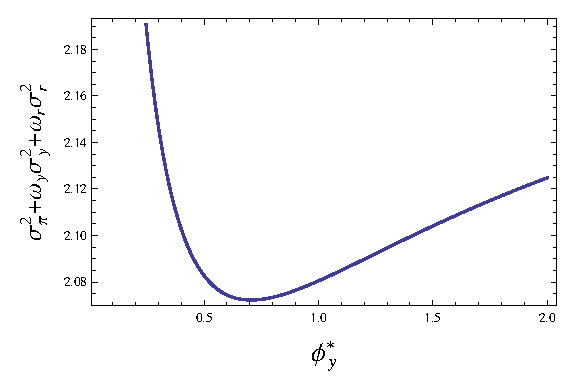
\includegraphics[width=3.2in]{varble09.eps}}\quad
        \subfigure[At the REE]
         {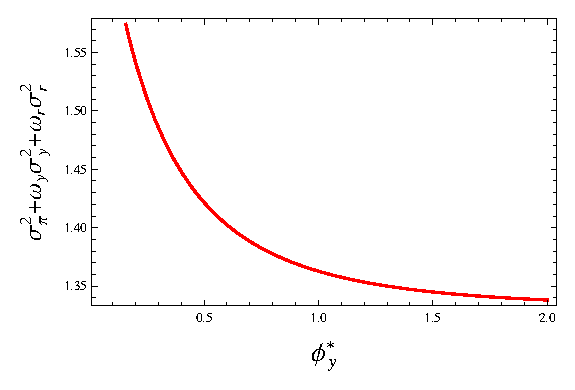
\includegraphics[width=3.2in]{varree09.eps}}}
   \end{center}
   \caption{\label{varopt09} Loss function along the optimal paths $(\phi_y^*, \phi_\pi^*)$ in Figure \ref{opt09} at the BLE (a) and REE (b). Parameters are: $\lambda=0.99, \varphi=1, \gamma=0.04,\rho=0.5, \frac{\sigma_2}{\sigma_1}=0.5$ and $\omega=0.9$.}
    \end{figure}
    
        We first examine monetary policy under BLE and REE at calibrated parameter values: as before in our calibration exercise, we consider the parameters $\lambda=0.99, \varphi=1, \gamma=0.04, \rho=0.5, \frac{\sigma_2}{\sigma_1}=0.5$ for both BLE and REE. This ensures that the economic structure is the same under both specifications, but the implied moments of inflation and output gap are different under BLE and REE.
       We first consider the case $\omega=0.9$, that is, the central bank places relatively large weight on inflation. Interestingly, we find that the optimal Taylor rule coefficients $(\phi_y^*, \phi_\pi^*)$ are finite under BLE in this case\footnote{
We first select a policy parameter domain (e.g. $[0,100]\times[1,100]$) and define a lattice with some small step ($e.g. \,\,0.01$). Then for each lattice point $(\phi_y, \phi_\pi)$, we find the BLE $(\beta_1^*(\phi_y, \phi_\pi), \beta_2^*(\phi_y, \phi_\pi))$ and the corresponding central bank's loss function $\omega\sigma_\pi^2+(1-\omega)\sigma_y^2$ at the BLE. Finally we interpolate the loss function with respect to $(\phi_y, \phi_\pi)$ to find the finite optimal values. It is easy to get analytic expressions of REE and the corresponding variances. In contrast, it is impossible to obtain analytic expressions of the optimal policy parameters under BLE and  therefore we have to rely on numerical approximations. We find consistent results using different ways to calculate the variances (i.e. based on (\ref{varyc}) and (\ref{varpic}) or computing the variances as in Appendix \ref{ACFn}).}.
As shown in Figure \ref{opt09}a, the corresponding optimal policy is $(\phi_y^*, \phi_\pi^*)=(0.9069, 4.8822)$.

This is different from REE, where there is no finite optimal policy except when measurement errors are considered, as shown in Boehm and House (2014). In fact, from Figure \ref{opt09} it can be seen that in the case $\phi_y^*$ is small enough (i.e. $<0.9069$) the coefficients $\phi_y^*$ and $\phi_\pi^*$ lie on a manifold and the loss function (\ref{varobj}) decreases gradually along the manifold within the region, which is similar to REE but with higher $\phi_\pi^*$. However, differently in the case $\phi_y^*>0.9069$, the loss function (\ref{varobj}) starts to increase, while in the REE the loss function (\ref{varobj}) still decreases as shown in Figure~\ref{varopt09}. That is to say, there exist finite optimal Taylor rule coefficients at the BLE, but not at the REE. This is mainly because at the BLE the actual law of motion has higher volatility (especially for inflation) than at the REE in most cases and minimizing the loss function, i.e. minimizing the weighted variances of output gap and inflation, requires balancing the different responses in terms of policy parameters $(\phi_y, \phi_\pi)$.


    
    \begin{figure}
    \begin{center}
        \mbox{\subfigure[Optimal policy ]
        {\includegraphics[width=3.2in]{optpolicyrho09.eps}}\quad
        \subfigure[Optimal manifold]
         {\includegraphics[width=3.2in]{optmanifrho.eps}}}
   \end{center}
   \label{optrho} 
   \caption{ Optimal policies at the BLE with respect to $\rho$ (a) and corresponding optimal manifolds for three different $\rho$ (connection points of solid and dotted curves corresponding to finite optimal policies) (b). Parameters are: $\lambda=0.99, \varphi=1, \gamma=0.04,\frac{\sigma_2}{\sigma_1}=0.5$ and $\omega=0.9$.}
    \end{figure}

Next we investigate how optimal monetary policy changes as the persistence of the underlying shocks is varied. At the REE with measurement error the finite coefficients $\phi_y^*$ and $\phi_\pi^*$ increase as the persistence of shocks grows within some range, see Boehm and House (2014). At the BLE, in addition to this, we find that when the persistence of exogenous shocks becomes sufficiently small with $\rho<0.4$, the finite coefficients $\phi_y^*$ and $\phi_\pi^*$ start increasing as shown in Figure \ref{optrho}a.  Furthermore, Figure \ref{optrho}b suggests that the optimal manifold always moves up as the persistence of shocks $\rho$ grows. The finite optimal policy lies at the point in the optimal manifold connecting the solid and dotted lines in Figure \ref{optrho}b. The location of the optimal point corresponding to finite optimal policies depends on the relative values of variances of output gap and inflation. In the case $\rho$ is large enough, the loss function is mainly dominated by the variance of inflation and hence the optimal policy $\phi_{\pi}^*$ grows quickly converging to $\infty$ and the slope of $\frac{\phi_\pi^*}{\phi_y^*}$ converging to a relatively large constant. Given the parameters, for small enough $\rho$, the loss function is mainly dominated by the variance of the output gap and also the finite optimal policy $\phi_y^*$ grows quickly converging to $\infty$ with a relatively small limit of $\frac{\phi_\pi^*}{\phi_y^*}$. Since both shock persistence parameters are fairly low in our estimation exercise, the optimal pair of coefficients for the U.S. data falls within this region as we will be discussed below. 

In a similar vein, if the weight on inflation $\omega$ is large enough, the loss function is dominated by the variance of inflation. Figure \ref{optomega}a suggests that the optimal policy is $\phi_\pi^*\to\infty$ and $\phi_y^*\to 0$ for $\omega=1$. Therefore, for large enough $\omega$, finite optimal policy $\phi_\pi^*$ increases while  $\phi_y^*$ decreases as $\omega$ grows, as shown in Figure \ref{optomega}. For small enough $\omega$, the variance of output gap plays a dominant role and hence the optimal manifold increases as $\omega$ grows (see Figure \ref{optomega}b). For a range of  $\omega$ values there exist finite optimal policies. As $\omega$ grows, the finite optimal policy $\phi_\pi^*$ first decreases and then increases, while $\phi_y^*$ decreases  within the range of existence of finite optimal policy.




\begin{figure}
    \begin{center}
        \mbox{\subfigure[Optimal policy ]
        {\includegraphics[width=3.2in]{optpolicyomega05.eps}}\quad
        \subfigure[Optimal manifold]
         {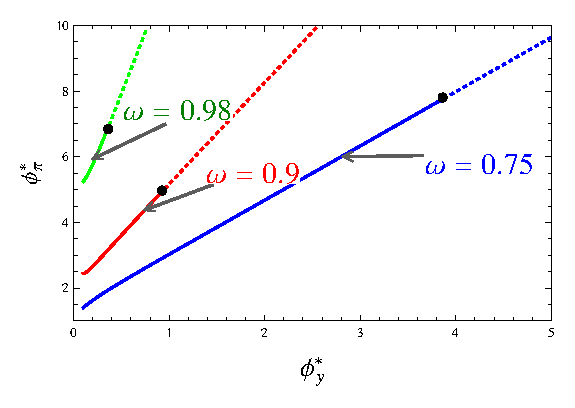
\includegraphics[width=3.2in]{optmanifomega.eps}}}
   \end{center}
   \caption{\label{optomega}  Optimal policies at the BLE with respect to $\omega$ (a) and corresponding optimal manifolds for three different $\omega$ (connection points of solid and dotted curves corresponding to finite optimal policies) (b) with the contemporaneous interest rate rule. Parameters are: $\lambda=0.99, \varphi=1, \gamma=0.04,\frac{\sigma_2}{\sigma_1}=0.5$ and $\rho=0.5$.}
    \end{figure}
    
    \begin{figure}
    \begin{center}
        \mbox{\subfigure[Optimal manifold]
        {\includegraphics[width=3.2in]{optpolicy.eps}}\quad
        \subfigure[Loss function along optimal manifold]
         {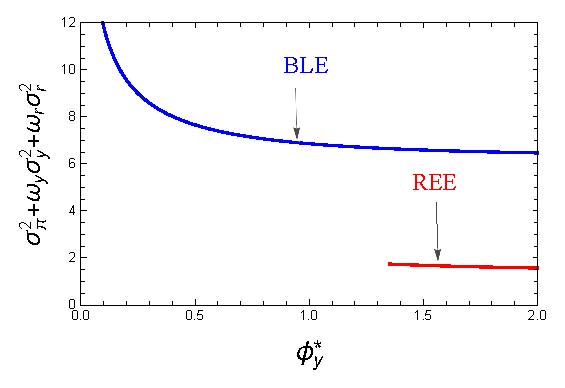
\includegraphics[width=3.2in]{optimalvar.eps}}}
   \end{center}
   \caption{\label{optbench} Optimal manifolds at the BLE and REE given each $\phi_y^*$ (a) and the corresponding loss function along the optimal paths (b) with the contemporaneous interest rate rule. Parameters are: $\lambda=0.99, \varphi=1, \gamma=0.04, \rho=0.5,
\frac{\sigma_2}{\sigma_1}=0.5$ and $\omega=0.5$.}
    \end{figure}

Next we investigate optimal monetary policy at our estimated parameter values. In this case the underlying economic structure is different under BLE and REE, while the moments of inflation and output gap are close under both specifications\footnote{Our analysis with the calibrated values is based on the expressions (3.15)-(3.18). This is no longer applicable since we add interest rate smoothing to our model and relax the assumption that exogenous shocks have the same persistence. Therefore we proceed by computing the fixed-points and the associated variances for each value of policy parameters using our Iterative E-stability algorithm.}. Similar to the calibration exercise, the finite pair of Taylor-coefficients does not exist under REE at the estimated parameter values. While the optimal Taylor-rule is still finite under BLE, the parameter values turn out to be arbitrarily large for both $\phi_y^{*}$ and $\phi_{\pi}^{*}$. This result is already suggested in Figure \ref{optrho}, which shows that optimal coefficients start to rapidly increase when the persistence of exogenous shocks becomes too small. Recalling that our estimated shock persistence parameters are $\rho_y=0.43$ and $\rho_{\pi}=0.32$, the variance of output gap quickly dominates over this region, leading to a large pair of optimal values. The first row of Figure \ref{optim_est} shows how the variances of inflation and output gap change as we vary the monetary policy coefficients over a more empirically plausible range: we vary $\phi_{\pi}$ over $[1,10]$ keeping $\phi_y$ fixed at its estimated value, and $\phi_y$ over $[0,10]$ keeping $\phi_{\pi}$ at its estimated value\footnote{Since the estimated interest rate smoothing parameters are slightly different, we fix this parameter at $\rho_r=0.85$ for both models to make the magnitudes of change in $\phi_{\pi}$ and $\phi_y$ equivalent under BLE and REE.}. It is readily seen that a relatively inactive monetary policy has a destabilizing effect under BLE: when $\phi_{\pi}$ falls below 1, or $\phi_y$ falls below $0.2$, the underlying BLE is destabilized and the variances grow exponentially. This is similar to the standard indeterminacy result under REE, but the negative consequences of a passive monetary policy on the economy are larger under BLE.  These two figures also  show that there is a clear trade-off between inflation and output gap variances when $\phi_{y}$ is kept fixed, while the trade-off with higher values of $\phi_y$ is too small over this empirically plausible range. This also implies that the arbitrarily large pair of optimal coefficients is driven by the small trade-off as $\phi_y$ is varied. 

%This is shown in the left panel of second row in Figure \ref{optim_est}, which plots the optimal values of $\phi_{\pi}$ under BLE and REE as a function of the inflation weight $\omega$.  Since the trade-off between inflation and output gap variance with varying $\phi_{\pi}$ is smaller under BLE, the resulting optimal coefficient also turns out larger  compared with REE for a wide range of weights $\omega$. With a weight of $0.9$,
%the optimal reaction coefficient is $3.57$ under BLE and $1.57$ under REE, with $\phi_{\pi}^{*}\rightarrow\infthy$ as $\omega \rightarrow 1 $ in both cases. 


 \begin{figure}
\centering
       \mbox{\subfigure[Variances w.r.t. $\phi_{\pi}$.]{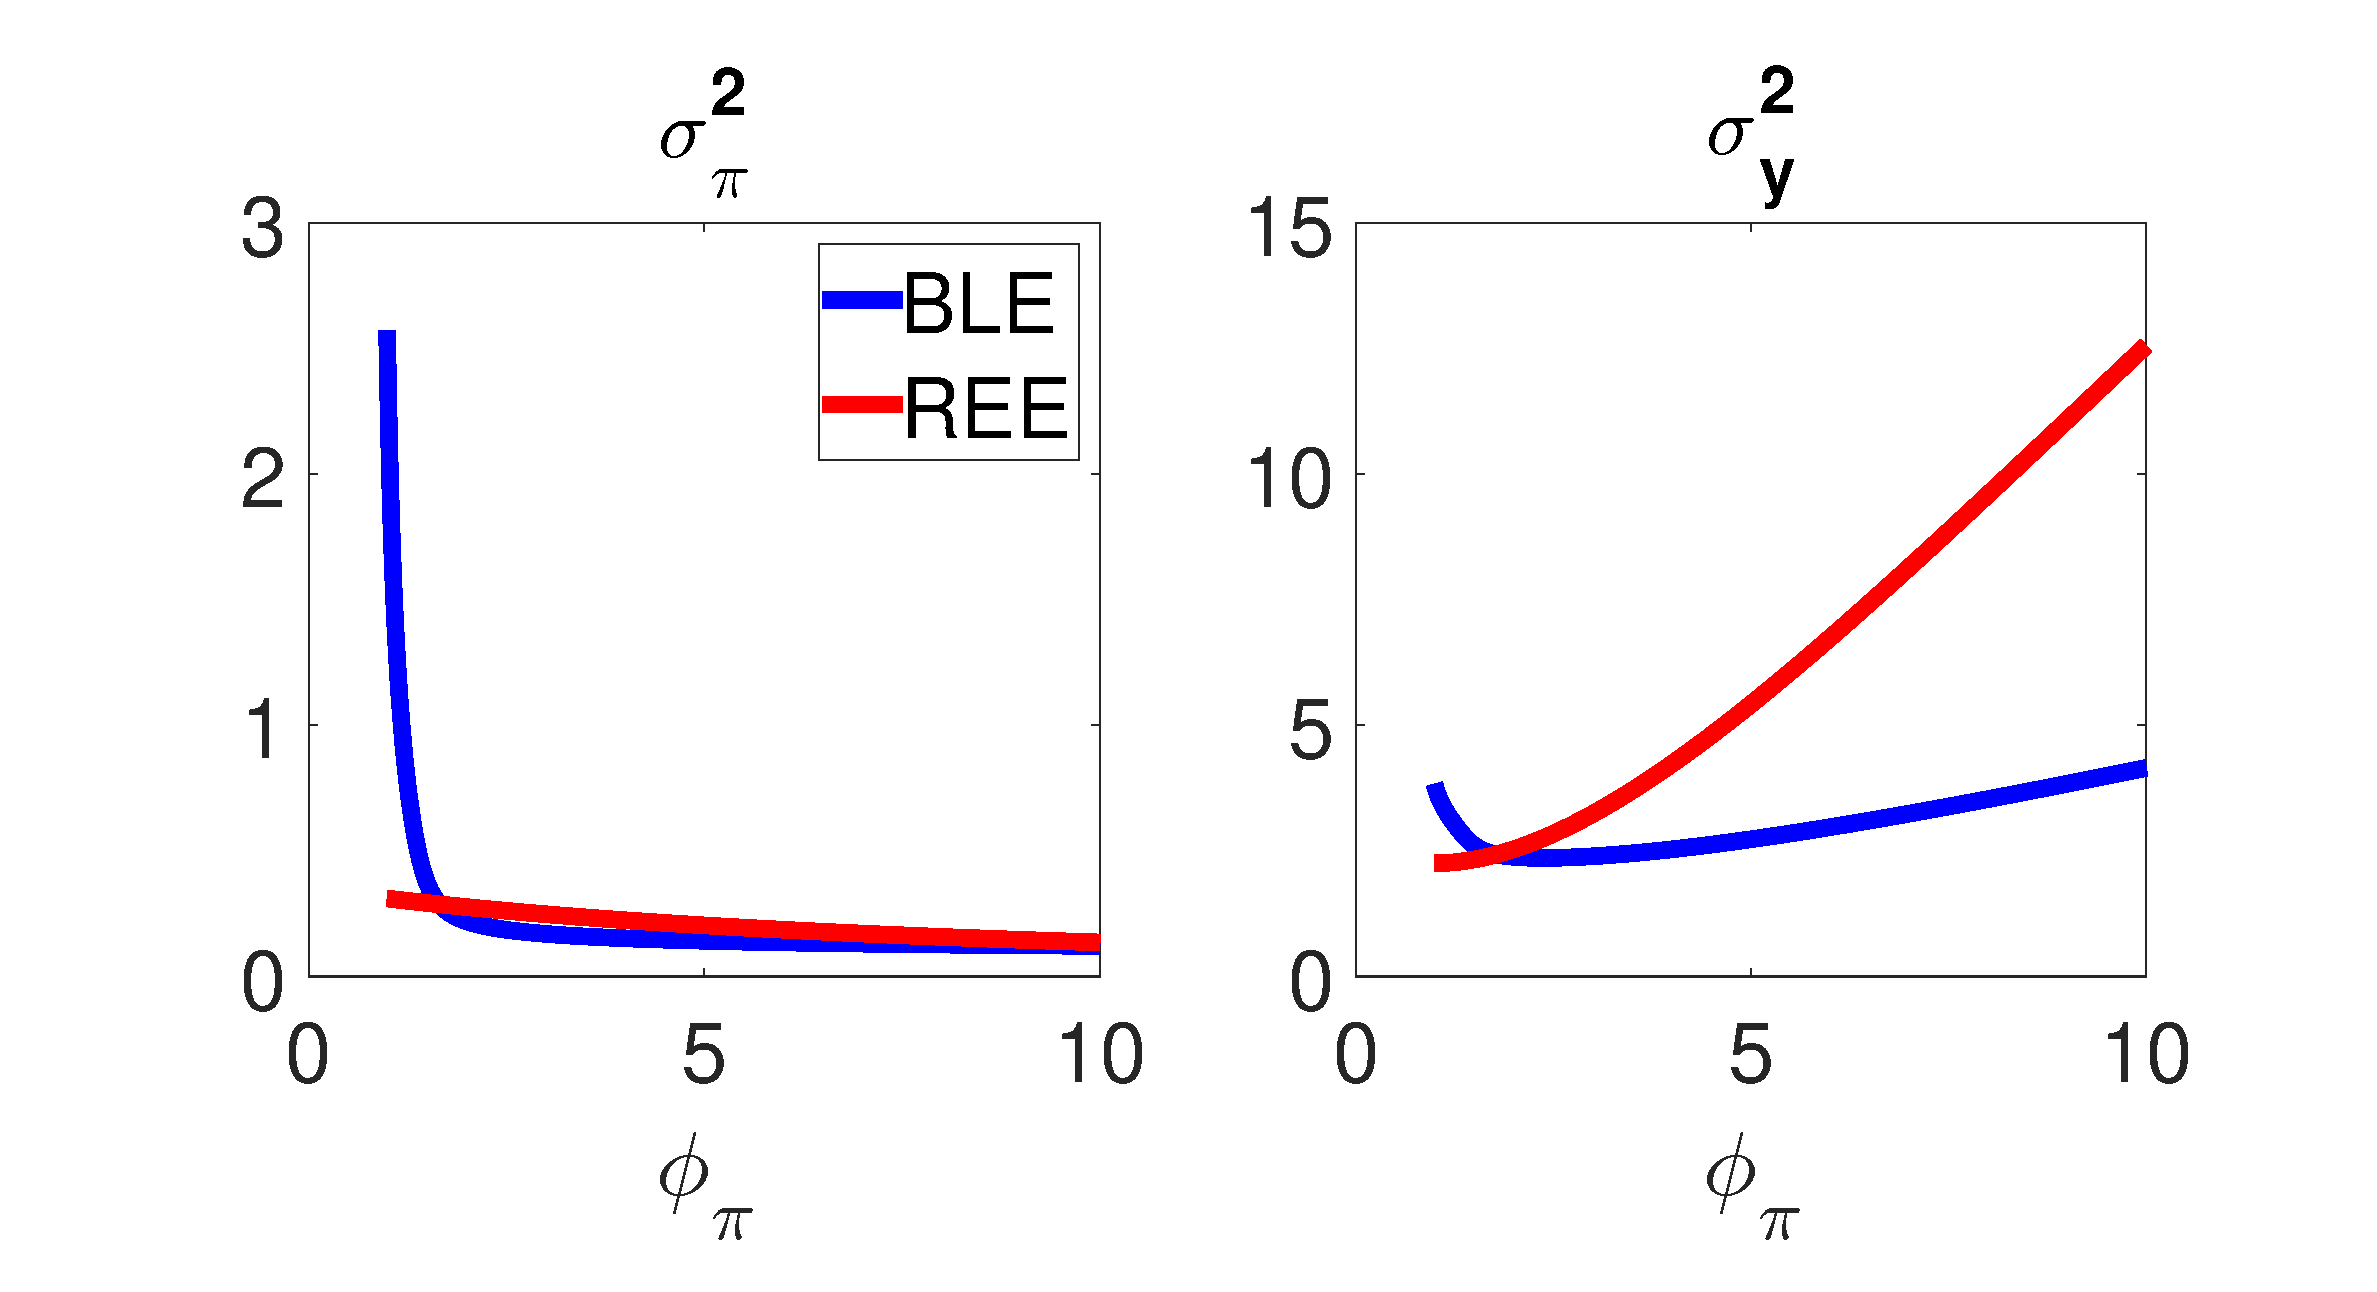
\includegraphics[scale=0.19]{optimal_policy_weight_pi_variances.pdf}}\quad
      \subfigure[Variances w.r.t. $\phi_{y}$.]{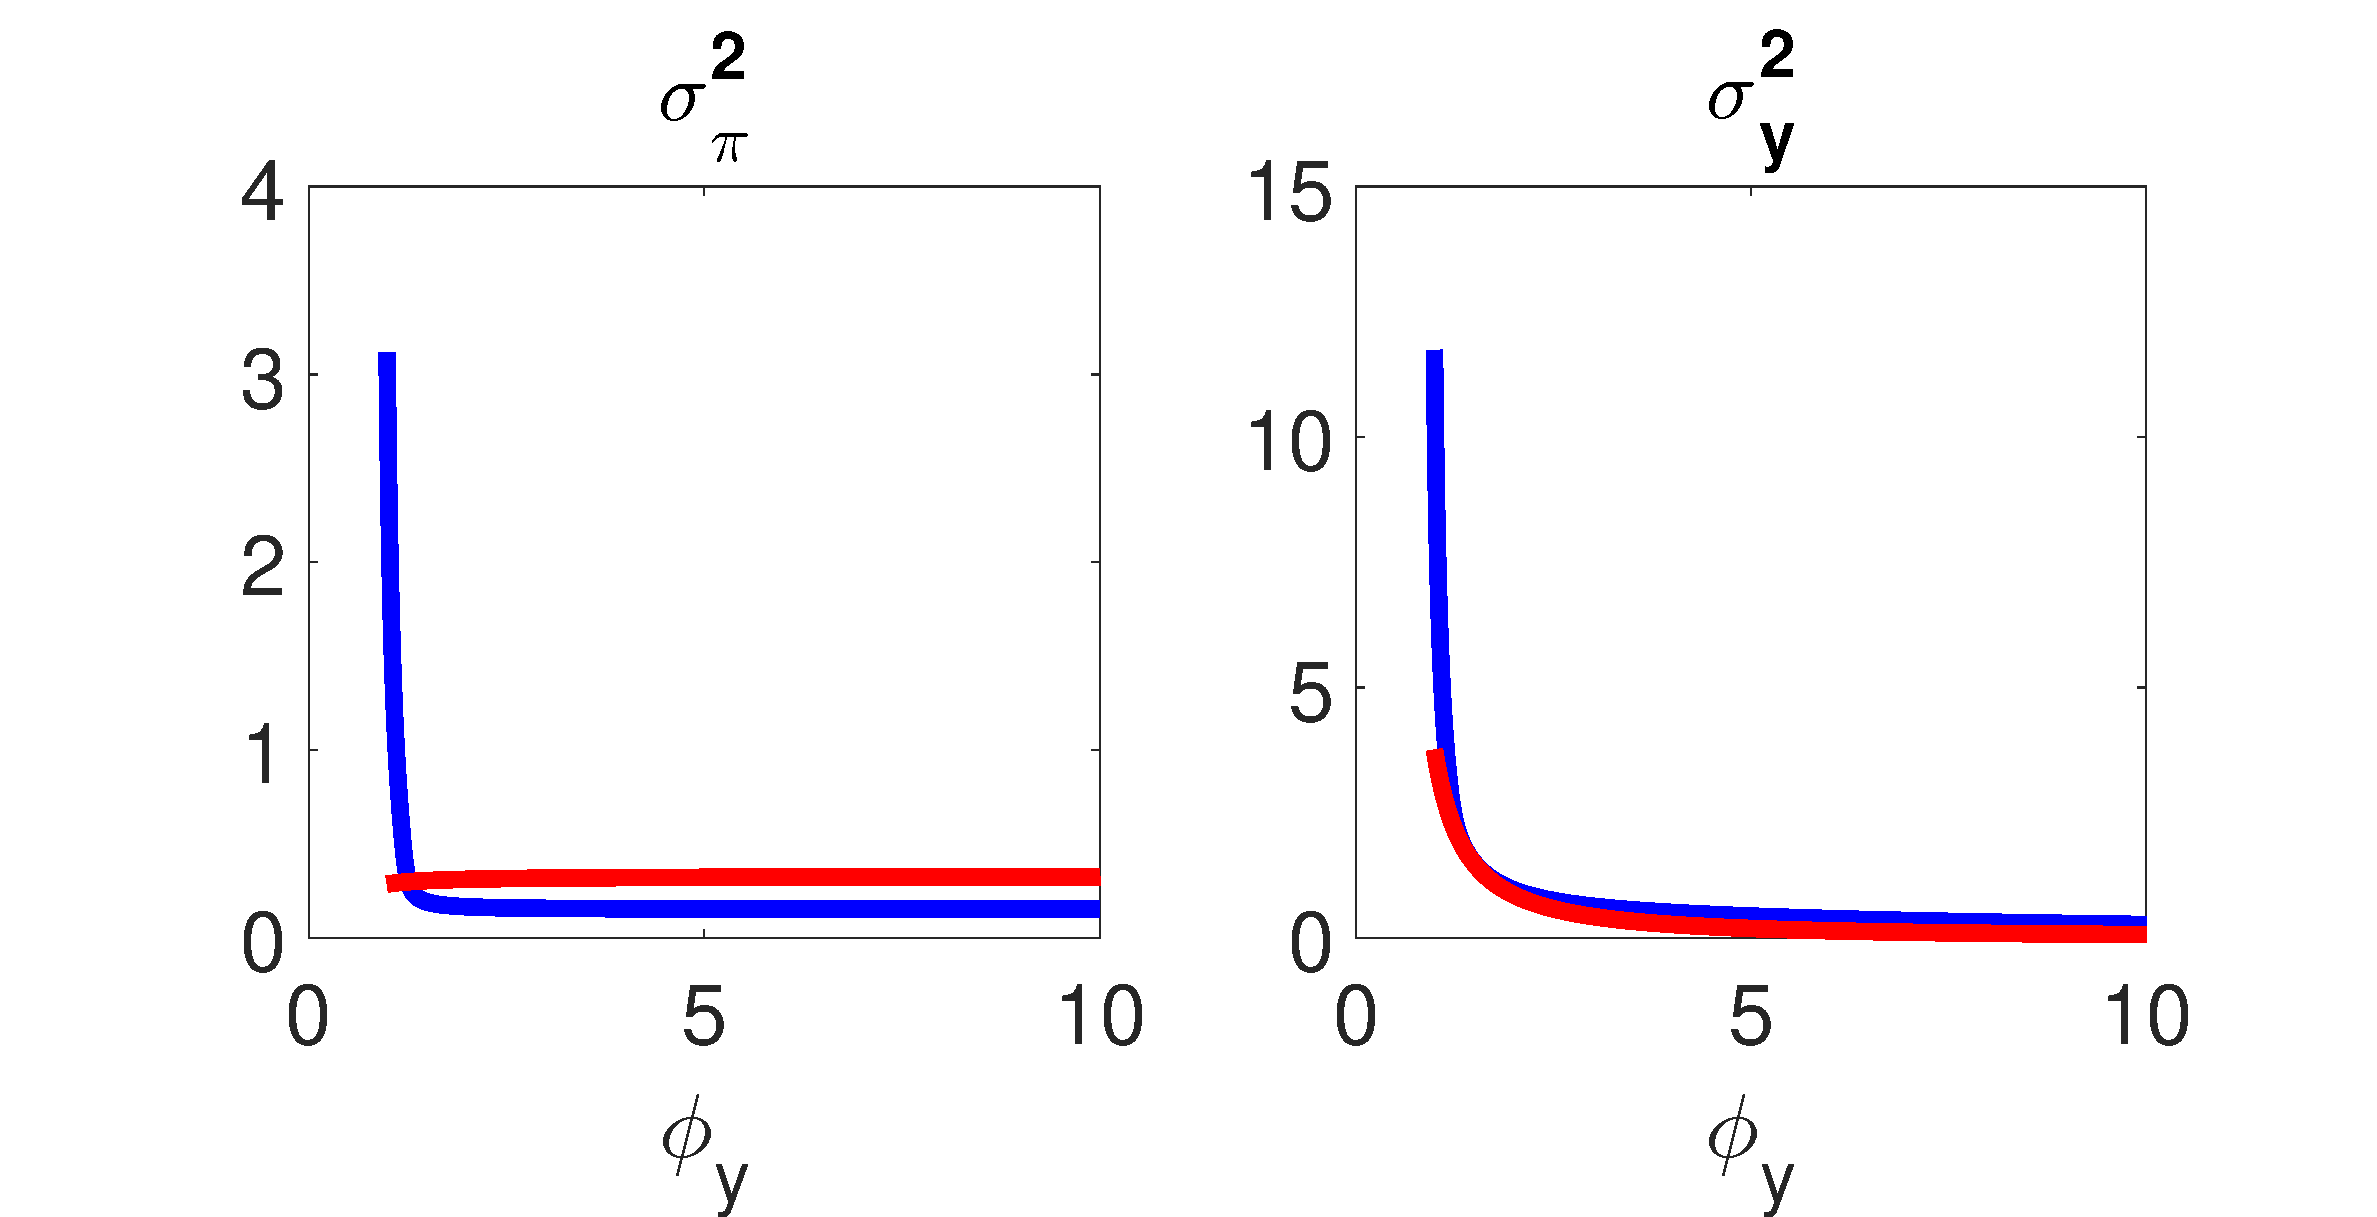
\includegraphics[scale=0.19]{optimal_policy_weight_y_variances.pdf}}}
    \caption{Variances of inflation and output gap as the monetary policy parameters are varied over the empirically plausible range. The blue and red lines show the variances under BLE and REE respectively.}
     \label{optim_est}
 \end{figure}




Figure \ref{imp_resp} shows the impulse responses of inflation and output gap to a monetary policy shock of the same size\footnote{The shock size is one standard deviation at the estimated parameter values for each case, which is the same under BLE and REE with $0.29$.}. Both the initial impact, as well as the cumulative impact of the shock are larger under BLE. This is because both the estimated slope of the Philips curve $\gamma$ and the intertemporal elasticity of substitution $\varphi$ are larger under BLE, leading to a stronger transmission channel of monetary policy shocks compared with REE. Furthermore the shock takes several quarters to reach its full impact under BLE, leading to hump-shaped responses for both inflation and output gap: this shows that the persistence amplification under BLE is also reflected in the system's response to an exogenous monetary policy shock. Together with Figure \ref{optim_est}, this  suggests that monetary policy has a stronger impact on the economy under BLE. 




 
 \begin{figure}
 \centering
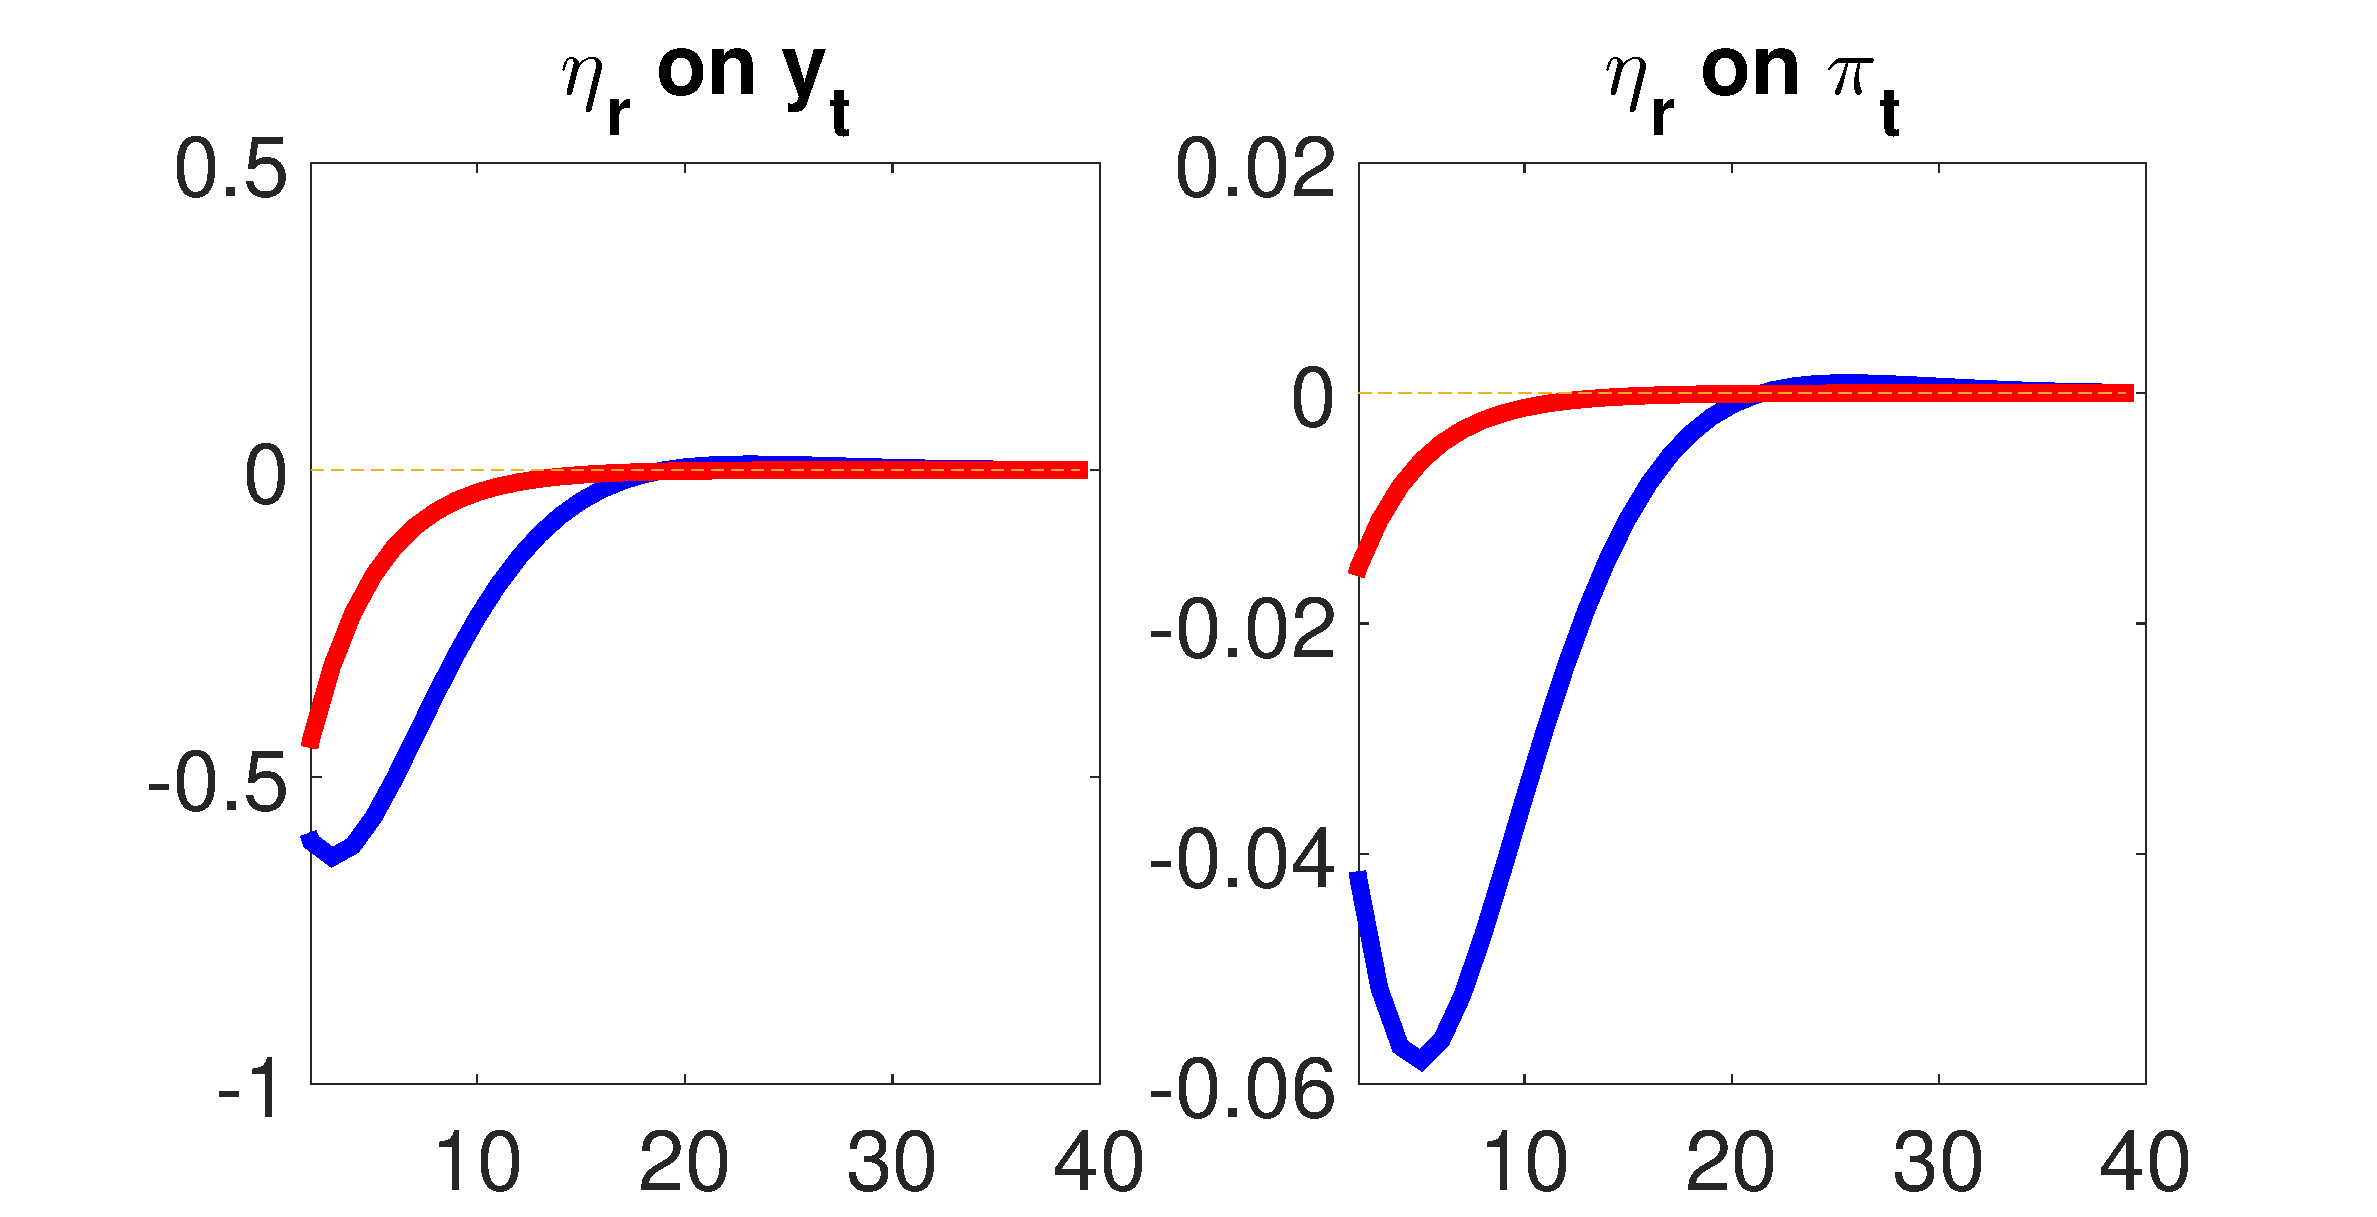
\includegraphics[scale=0.25]{nkpc_irfs_comparison.pdf} 
\caption{Impulse responses to a monetary policy shock of one standard deviation. The blue and red lines show the responses under BLE and REE respectively.}
\label{imp_resp}
\end{figure}
             
 We close this section with an illustration of how multiplicity of equilibria can arise under BLE when monetary policy parameters are varied. In all calibration and estimation exercises that we discussed so far, the underlying BLE is unique. However, multiple stable BLE can arise for certain combinations of parameter values. One such case can be observed when we set the parameter values to their CBO-based output gap estimations as given in Table \ref{nkm_alt_gap}, and vary the values of monetary policy parameters. 

 \begin{figure}
\centering        
             \mbox{\subfigure[Variances $\sigma_y^2$ and $\sigma_{\pi}^2 $ w.r.t. $\phi_{y}$]{\includegraphics[scale=0.19]{phi_y_variance.pdf}   }} 
 \mbox{\subfigure[Variances $\sigma_y^2$ and $\sigma_{\pi}^2 $ w.r.t. $\phi_{y}$]{\includegraphics[scale=0.19]{phi_pi_variance.pdf}}} \\  
            \caption{Optimal Policy under BLE and REE at the estimated parameter values.}
            \label{mult_eqm}
\end{figure}  

In this case the estimated Philips curve slope $\gamma$ is smaller at $0.024$ compared with our benchmark estimation with $\gamma=0.035$. Figure \ref{optim_est} illustrates how inflation and output gap variances change as we vary the monetary policy coefficients $\phi_y \in [0.25, 0.5]$ and $\phi_{\pi} \in [1,1.75]$ in this case. While the change in variances follow the same overall pattern as in the benchmark case, we observe two co-existing E-stable BLE over a small range of parameter values. The underlying BLE is unique at the estimated parameter values, but as the reaction coefficients become smaller, with $\phi_y<0.33$ or $\phi_{\pi}<1.3$, another BLE with higher variance and higher persistence for both inflation and output gap becomes stable and there is a range of parameter values where these two stable BLE co-exist. For smaller values of reaction coefficients,
with $\phi_y < 0.31$ or $\phi_{\pi}<1.1$, 
the low persistence/low variance equilibrium becomes unstable and only the high-variance equilibrium remains. These results suggest that, for certain parameter combinations, there is another important role for monetary policy in terms of ensuring that such high volatility equilibria are destabilized, which is only possible with a sufficiently active policy rule. In our example multiplicity of equilibria is driven by a flatter Philips curve compared to our benchmark case, but similar results can arise when other structural parameters are varied, such as the exogenous shock persistence parameters $\rho_y$ and $\rho_{\pi}$, or the intertemporal elasticity of substitution $\varphi$. \\





\section{Optimal Monetary Policy}
\label{sec:MonPol}

Our results so far show that BLE generally provides a better model fit than REE for the 3-equation New Keynesian model, with important differences in the estimated structural parameters and the propagation mechanism under BLE and REE. This leaves an important question for the optimal Taylor rule at BLE: how do the optimal values of Taylor rule parameters differ under BLE and REE? In this section we answer this question by considering optimal monetary policy under both calibrated and estimated parameter values.
%Our results so far illustrate that, when BLE and REE are examined under the same set of calibrated parameter values, BLE are characterized by persistence and volatility amplification, with much higher persistence and variance in output gap and inflation compared with REE. As a consequence, there are substantial differences in the estimated parameters and propagation structure when the 3-equation model is evaluated under BLE and REE. This leaves an important question for the optimal Taylor-rule parameters at the BLE. As shown in Boehm and House (2014), at the REE when the output gap and
%inflation are observed without error, it is typically optimal to respond infinitely strongly to observed deviations from the central bank's targets, while with measurement error the optimal Taylor rule coefficients are finite.
%How do the optimal values of Taylor rule parameters differ between the BLE and REE? In this section we try to answer this question by considering optimal monetary policy under both calibrated and estimated parameter values. 
We assume that the central bank wishes to minimize an expected loss function $E[L]$ in terms of the discounted sum of weighted squared inflation, output gap and interest rate
\begin{equation}
E[L]=(1-\vartheta)E\Big[\Sigma_{t=0}^\infty  \vartheta^t[\omega_{\pi} \pi_t^2+\omega_yy_t^2+\omega_r r_t^2] \Big]=\omega_{\pi} \sigma_\pi^2+\omega_y\sigma_y^2+\omega_r\sigma_r^2,\label{varobj}
\end{equation}
where $\omega_i$, $i \in \{\pi,y,r \}$ is the relative weight that the central bank places on inflation, output gap and interest rate respectively. The stabilization objective for inflation and output gap is a standard assumption in the literature, see e.g.  Boehm and House (2014), Evans and Honkapohja (2003) and Woodford (2003). The weight on interest rate variance can be motivated by different interpretations: Woodford (1999) and Giannoni (2014) suggest that it can proxy for welfare costs of transactions and/or an approximation on the zero lower bound on nominal interest rates, while Caplin and Leahy (1996) suggest that it can represent a gradual learning process for the central bank that is uncertain about the consequences of interest rate fluctuations. 

%From the equations (\ref{varyapp}) and (\ref{varpiapp}) in Appendix \ref{acfnkc},
Based on our calculations, the unconditional moments under BLE are given as 
\begin{eqnarray}
\sigma_y^2&=&\frac{\widetilde{g}_1}{(1+\gamma\varphi\phi_\pi+\varphi\phi_y)^2(1-\rho^2)(1-\rho\lambda_1)(1-\rho\lambda_2)(1-\lambda_1^2)(1-\lambda_2^2)(1-\lambda_1\lambda_2)}, \label{varyc}\\
\sigma_\pi^2&=&\frac{\widetilde{g}_2}{(1+\gamma\varphi\phi_\pi+\varphi\phi_y)^2(1-\rho^2)(1-\rho\lambda_1)(1-\rho\lambda_2)(1-\lambda_1^2)(1-\lambda_2^2)(1-\lambda_1\lambda_2)}, \label{varpic}\\
\sigma_r^2&=&\phi_y^2\sigma_y^2+\phi_\pi^2\sigma_\pi^2+2\phi_y\phi_\pi E(y_t\pi_t),\label{varrc}
\end{eqnarray}
where $\widetilde{g}_1$, $\widetilde{g}_2$, $\lambda_1$, $\lambda_2$ are given by the equations (\ref{gyvar}), (\ref{gpivar}), (\ref{lambdatr}) and (\ref{lambdade}), and
\begin{eqnarray*}
E(y_t\pi_t)&=&\Big(-\sigma_y^2\gamma\big(-(1+\gamma\varphi\phi_\pi+\varphi\phi_y)(1+\gamma\varphi\phi_\pi+\varphi\phi_y+\beta_1^2\rho)+\beta_2^4\lambda(1+\gamma\varphi\phi_\pi\\
&&+\varphi\phi_y+\beta_1^2\rho)(\lambda+\gamma\varphi+\lambda\varphi\phi_y)+\beta_2^2\rho[\beta_1^4\lambda+\beta_1^2\lambda\rho(1+\gamma\varphi\phi_\pi+\varphi\phi_y)+\gamma\varphi\\
&&(-1+\lambda \phi_\pi)(1+\gamma\varphi\phi_\pi+\varphi\phi_y)]-\beta_1^2\beta_2^6\lambda^2\rho(\beta_1^2\lambda+\rho(\lambda+\gamma\varphi+\lambda\varphi\phi_y))\big)+\sigma_{\pi}^2\varphi\\
&&\big(-\phi_\pi(1+\gamma\varphi\phi_\pi+\varphi\phi_y)[-\beta_1^4-\beta_1^2\gamma\rho\varphi\phi_\pi+(1+\varphi\phi_y)(1+\gamma\varphi\phi_\pi+\varphi\phi_y)]+\beta_1^2\beta_2^6\lambda\rho\\
&&[-\gamma\varphi(-\beta_1^2+\rho+\rho\varphi\phi_y)+\lambda\rho(\beta_1^4-(1+\varphi\phi_y)^2)]+\beta_2^4\big(\gamma\varphi(1-\beta_1^2\rho+\varphi\phi_y)(1+\gamma\varphi\phi_\pi\\
&&+\varphi\phi_y)+\lambda(-1+\beta_1^2\rho-\varphi(\gamma\phi_\pi+\phi_y))(\beta_1^4-(1+\varphi\phi_y)^2)+\beta_1^2\lambda^2\rho\phi_\pi(-\beta_1^4+\\
&&(1+\varphi\phi_y)^2)\big)+\beta_2^2\rho[-\beta_1^6\lambda\rho\phi_\pi+\beta_1^2\lambda\rho\phi_\pi(1+\varphi\phi_y)(1+\gamma\varphi\phi_\pi+\varphi\phi_y)-(-1+\lambda\phi_\pi)\\
&&(1+\varphi\phi_y)^2(1+\gamma\varphi\phi_\pi+\varphi\phi_y)+\beta_1^4(-1-\varphi(\gamma\phi_\pi+\varphi_y)+\lambda(\phi_\pi+\varphi\phi_\pi\phi_y))]\big)\Big)\Big/  \\
&& \Big((-1+\rho^2)(-1+\beta_1^2\beta_2^2\lambda-\varphi(\gamma\phi_\pi+\phi_y))(1+\beta_1^2\rho(-1+\beta_2^2\lambda\rho)+\gamma\varphi\phi_\pi+\varphi\phi_y\\
&&-\beta_2^2\rho(\lambda+\gamma\varphi+\lambda\varphi\phi_y))\big(\beta_1^4(-1+\beta_2^4\lambda^2)+2\beta_1^2\beta_2^2\gamma\varphi(-1+\lambda\phi_\pi)+(1+\gamma\varphi\phi_\pi+\varphi\phi_y)^2\\
&&-\beta_2^4(\lambda+\gamma\varphi+\lambda\varphi\phi_y)^2\big)\Big).
\end{eqnarray*}
In the following we study the optimal values  $(\phi_y^*, \phi_\pi^*)$ that minimize the central bank's loss function (\ref{varobj}) at the BLE, where $\beta_1^*$ and $\beta_2^*$ are at the BLE   ($\beta_1^*, \beta_2^*$).

\begin{figure}
    \begin{center}
     \includegraphics[width=3.2in]{optpolicy09.eps}
     \end{center}
   \caption{\label{opt09} Optimal policies at the BLE and at the REE. Parameters are: $\lambda=0.99, \varphi=1, \rho=0.5,\gamma=0.04,\sigma_y=1,\sigma_{\pi}=0.5$ and $\omega_y=0.1,\omega_r=0.05$.}
    \end{figure}


\begin{figure}
    \begin{center}
        \mbox{\subfigure[At the BLE ]
        {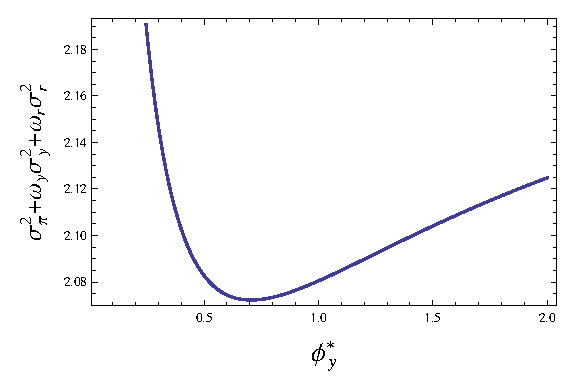
\includegraphics[width=3.2in]{varble09.eps}}\quad
        \subfigure[At the REE]
         {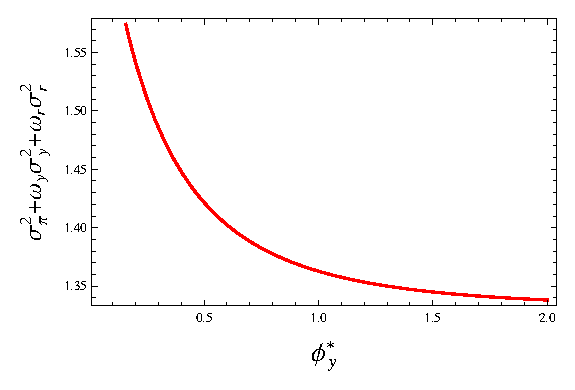
\includegraphics[width=3.2in]{varree09.eps}}}
   \end{center}
   \caption{\label{varopt09} Loss function along the optimal paths $(\phi_y^*, \phi_\pi^*)$ in Figure \ref{opt09} at the BLE (a) and REE (b). Parameters are:  $\lambda=0.99, \varphi=1, \rho=0.5,\gamma=0.04,\sigma_y=1,\sigma_{\pi}=0.5$ and $\omega_y=0.1,\omega_r=0.05$.}
    \end{figure}
    
        We first examine monetary policy under BLE and REE at calibrated parameter values: as before in our calibration exercise, we consider the parameters $\lambda=0.99, \varphi=1, \gamma=0.04, \rho=0.5, \frac{\sigma_{\pi}}{\sigma_y}=0.5$ for both BLE and REE. This ensures that all structural parameters are the same under both specifications, hence the data generating process only differs in terms of the expectation formation rule. The analysis for calibrated parameters provides some insight on how optimal monetary policy under BLE depends on model parameters, particularly the persistence of shocks. As we saw in previous sections, there are important differences in the moments of endogenous variables due to volatility and persistence amplification at BLE. In particular, the implied variances of inflation, output gap and interest rate are different under BLE and REE at these parameter values. Following Woodford (1999) and Giannoni (2014), we normalize the weight on inflation to $\omega_{\pi}=1$. 
        We first focus on a special case with $\omega_y=0.1$ and $\omega_r=0.05$, that is, the central bank places a relatively large weight on inflation and a small one on interest rates. The small weight on interest rates allows us to first focus on the trade-off between inflation and output gap stabilization. We leave the discussion of how optimal policy depends on these policy weight for the more empirically relevant case of estimated parameters. 

    Interestingly, we find that the optimal Taylor rule coefficients $(\phi_y^*, \phi_\pi^*)$ are finite under BLE in this case\footnote{
We first select a policy parameter domain (e.g. $[0,100]\times[1,100]$) and define a lattice with some small step ($e.g. \,\,0.01$). Then for each lattice point $(\phi_y, \phi_\pi)$, we find the BLE $(\beta_1^*(\phi_y, \phi_\pi), \beta_2^*(\phi_y, \phi_\pi))$ and the corresponding central bank's expected loss function $E[L]$ at the BLE. Finally we interpolate the loss function with respect to $(\phi_y, \phi_\pi)$ to find the finite optimal values. It is easy to get analytic expressions of the variances and optimal policy parameters under REE. In contrast, it is impossible to obtain analytic expressions of the optimal policy parameters under BLE and  therefore we have to rely on numerical approximations. We find consistent results using different ways to calculate the variances (i.e. based on (\ref{varyc}) and (\ref{varpic}) or computing the variances as in Appendix \ref{ACFn}).}.
As shown in Figure \ref{opt09}, the corresponding optimal policy is $(\phi_y^*, \phi_\pi^*)=(0.9069, 4.8822)$. This is different from REE, where there is no finite optimal policy except when measurement errors are considered, as shown in Boehm and House (2014)\footnote{The loss function considered in Boehm and House (2014) does not include interest rate variance. Including interest rates in our loss function here does not affect the result that optimal policy at REE does not exit as long as $\omega_r$ remains sufficiently small. Optimal policy becomes finite when $\omega_r$ is sufficiently large, these cases are discussed under the estimated parameter values.}. In fact, from Figure \ref{opt09} it can be seen that in the case $\phi_y^*$ is small enough (i.e. $<0.9069$) the coefficients $\phi_y^*$ and $\phi_\pi^*$ lie on a manifold and the loss function (\ref{varobj}) decreases gradually along the manifold within this region, which is similar to REE but with higher $\phi_\pi^*$. However, for $\phi_y^*>0.9069$, the loss function (\ref{varobj}) starts to increase, while in the REE the loss function (\ref{varobj}) still decreases as shown in Figure~\ref{varopt09}. That is to say, there exist finite optimal Taylor rule coefficients at the BLE, but not at the REE. This is mainly because at the BLE the actual law of motion has higher variance than at the REE for most variables (especially inflation) and minimizing the loss function, i.e. minimizing the weighted variances of output gap and inflation, requires balancing the different responses in terms of policy parameters $(\phi_y, \phi_\pi)$.


  \begin{figure}
    \begin{center}
        \mbox{\subfigure[Optimal policy ]
        {\includegraphics[width=3.2in]{optpolicyrho09.eps}}\quad
        \subfigure[Optimal manifold]
         {\includegraphics[width=3.2in]{optmanifrho.eps}}}
   \end{center}
   \caption{\label{optrho}  Optimal policies at the BLE with respect to $\rho$ (a) and corresponding optimal manifolds for three different $\rho$ (connection points of solid and dotted curves corresponding to finite optimal policies) (b). Parameters are: $\lambda=0.99, \varphi=1, \gamma=0.04,\sigma_y=1,\sigma_{\pi}=0.5$ and $\omega_y=0.1,\omega_r=0.05$.}
    \end{figure}


Next we investigate how optimal monetary policy changes as the persistence of the underlying shocks is varied. At the REE with measurement error the finite coefficients $\phi_y^*$ and $\phi_\pi^*$ increase as the persistence of shocks grows within some range, see Boehm and House (2014). At the BLE, in addition to this, we find that when the persistence of exogenous shocks becomes sufficiently small with $\rho<0.4$, the finite coefficients $\phi_y^*$ and $\phi_\pi^*$ increase in a small region as shown in Figure \ref{optrho}a, before they start decreasing again. Furthermore, Figure \ref{optrho}b suggests that the optimal manifold always moves up as the persistence of shocks $\rho$ grows. The finite optimal policy lies at the point in the optimal manifold connecting the solid and dotted lines in Figure \ref{optrho}b. The location of the optimal point corresponding to finite optimal policies depends on the relative values of variances of inflation, output gap and interest rate. In the case $\rho$ is large enough, the loss function is mainly dominated by the variance of inflation and hence the optimal policy $\phi_{\pi}^*$ grows quickly converging to $\infty$ and the slope of $\frac{\phi_\pi^*}{\phi_y^*}$ converging to a relatively large constant. As $\rho$ becomes smaller, the variance of interest rate starts to play a more dominant role, which leads to smaller values for both ${\phi_\pi^*} $ and ${\phi_y^*}$. The region with small values of $\rho$ is the most relevant for U.S. data since both shock persistence parameters are low at the BLE in our estimation exercises.

%Are the finite optimal policies more aggressive in response to more persistent underlying shocks? At the REE with measurement error the finite coefficients $\phi_y^*$ and $\phi_\pi^*$ increase as the persistence of shocks grows within some range, see Boehm and House (2014). But at the BLE, we find that for relatively large $\rho$ the finite coefficients $\phi_y^*$ and $\phi_\pi^*$ increase as the persistence $\rho$ of shocks grows, while for some smaller range of $\rho$ the finite coefficients $\phi_y^*$ and $\phi_\pi^*$ first increases and then decrease as the persistence $\rho$ of shocks grows, as shown in Figure \ref{optrho}a. Furthermore, Figure \ref{optrho}b suggests that the optimal manifold always moves up as the persistence of shocks $\rho$ grows. The finite optimal policy lies at the point in the optimal manifold connecting the solid and dotted lines in Figure \ref{optrho}b. The location of the optimal point corresponding to finite optimal policies depends on the relative values of variances of output gap and inflation. In the case $\rho$ is large enough, the loss function is mainly dominated by the variance of inflation and hence the optimal policy $\phi_{\pi}^*$ grows quickly converging to $\infty$ and the slope of $\frac{\phi_\pi^*}{\phi_y^*}$ converging to a relatively large constant. For relatively small $\rho$, the effect of $\rho$ with interest variances in the objective function is different from the traditional case without interest variance in the objective function. In any case, the corresponding loss function at the optimal policies at the BLE increases with respect to $\rho$, for example $=\omega\sigma_\pi^2+\omega_y\sigma_y^2+\omega_r\sigma_r^2= 0.5855, 2.0723, 12.8143$ for $\rho=0.35, 0.5, 0.75$, respectively.

%In a similar vein, if the weight on inflation $\omega$ is large enough, the loss function is dominated by the variance of inflation. Figure \ref{optomega}a suggests that the optimal policy is $\phi_\pi^*\to\infty$ and $\phi_y^*\to 0$ for $\omega=1$. Therefore, for large enough $\omega$, finite optimal policy $\phi_\pi^*$ increases while  $\phi_y^*$ decreases as $\omega$ grows, as shown in Figure \ref{optomega}. For small enough $\omega$, the variance of output gap plays a dominant role and hence the optimal manifold increases as $\omega$ grows (see Figure \ref{optomega}b). For a range of  $\omega$ values there exist finite optimal policies. As $\omega$ grows, the finite optimal policy $\phi_\pi^*$ first decreases and then increases, while $\phi_y^*$ decreases  within the range of existence of finite optimal policy.


%Now consider the case $\omega_y=1,\omega_r=0.05$ with all the other parameters as before. In this case, we find that the optimal monetary policies at the BLE are such that  that $\phi_y^*\to \infty$ and $\phi_\pi^*$ lies at a manifold as shown in Figure \ref{optbench}a\footnote{Although the figure only shows the range of $\phi_y^*$ within $[0,2]$, we checked for a larger range  $\phi_y^*\in [0,100]$ and still can not find a finite optimal policy. The corresponding loss function (\ref{varobj}) keeps decreasing even if the decreasing speed is very slow for large $\phi_y^*$. }.
%However, the loss function (\ref{varobj}) along the optimal line varies only little after $\phi_y^*>0.5$, as shown in Figure \ref{optbench}b. In fact, if the policy $\phi_y^*=0.5$, then the corresponding $\phi_\pi^*\approx 1.5$, which suggests that the traditional choice of $(\phi_y, \phi_\pi)=(0.5, 1.5)$ is reasonable and nearly optimal under the BLE framework when the weights on inflation and output gap are equal and the weight on interest rate is small enough. In addition, compared with the REE, all $(\phi_y^*, \phi_\pi^*)$ in the optimal manifold at the BLE satisfy the determinacy condition, which is also a sufficient condition for the existence of BLE, while only for sufficient large $\phi_y^*(>1.35)$ does the corresponding $(\phi_y^*, \phi_\pi^*)$ in the optimal manifold at the REE satisfy the determinacy condition. Furthermore it is easy to see that given $\phi_y^*>1.35$, $\phi_\pi^*$ in the manifold at the BLE is much greater than at the REE. Therefore, although the optimal policy at the BLE with $\omega_y=1,\omega_r=0.05$ is also $\phi_y^*\to \infty$ and $\phi_\pi^*$ lies at a manifold, the optimal manifold at the BLE is much higher than at the REE, which is consistent with higher persistence and higher volatility of inflation compared to the output gap at the BLE.


\begin{figure}
    \begin{center}
        \mbox{\subfigure[Optimal policy ]
        {\includegraphics[width=3.2in]{optpolicyomega05.eps}}\quad
        \subfigure[Optimal manifold]
         {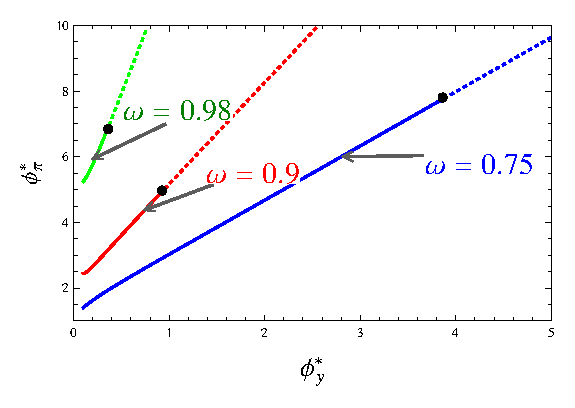
\includegraphics[width=3.2in]{optmanifomega.eps}}}
   \end{center}
   \caption{\label{optomega}  Optimal policies at the BLE with respect to $\omega$ (a) and corresponding optimal manifolds for three different $\omega$ (connection points of solid and dotted curves corresponding to finite optimal policies) (b) with the contemporaneous interest rate rule. Parameters are: $\lambda=0.99, \varphi=1, \gamma=0.04,\frac{\sigma_y}{\sigma_{\pi}}=0.5$ and $\rho=0.5$.}
    \end{figure}
    
%=======================================================================================================   
\begin{sidewaystable}
\small
\begin{tabular}{lll|ll|ll|lllll|lllll}
$\omega_{\pi}$ & $\omega_{y}$ & $\omega_{r}$ & BLE &  & REE &  & BLE &  &  &  &  & REE &  &  &  &  \\
 &  &  & $\phi_y^{*}$ & $\phi_{\pi}^{*}$ & $\phi_y^{*}$ & $\phi_{\pi}^{*}$ & $Var(\pi_t)^{*}$ & $Var(y_t)^{*}$ & $Var(r_t)^{*}$ & $E[L^{*}]$ & $\Delta E[L^{*}]$ & $Var(\pi_t)^{*}$ & $Var(y_t)^{*}$ & $Var(r_t)^{*}$ & $E[L^{*}]$ & $\Delta E[L^{*}]$ \\
\hline
\hline
1 & 0.1 & 0.05 & 3.94 & 3.49 & 2.74 & 4.43 & 0.14 & 0.49 & 1.06 & 0.24 & 58 \% & 0.31 & 0.19 & 1.41 & 0.40 & 27 \%\\
1 & 0.048 & 0.236 & 1.67 & 1.56 & 0.94 & 0.75 & 0.16 & 0.82 & 0.61 & 0.34 & 32 \% & 0.32 & 1.40 & 0.71 & 0.55 & 1 \%\\
\hline
1 & 0.25 & 0 & 15 & 13.33 & 4.35 & 15 & 0.13 & 0.27 & 2.8 & 0.18 & 82 \% & 0.32 & 0.04 & 1.8 & 0.33 & 60 \% \\
1 & 0.20 & 0.05 & 6.67 & 3.94 & 2.64 & 8.51 & 0.14 & 0.35 & 1.45 & 0.28  & 68 \% & 0.32 & 0.07 & 1.61 & 0.41 & 46 \% \\
1 & 0.15 & 0.09 & 3.33 & 2.27 & 1.64 & 3.80 & 0.15 & 0.53 & 0.89 & 0.31  & 58 \% & 0.32 & 0.2 & 1.31 & 0.48 & 31 \% \\
1 & 0.10 & 0.15 & 2.42 & 1.82 & 1.25 & 1.96 & 0.15 & 0.64 & 0.73 & 0.32  & 48  \% & 0.32 & 0.46 & 1.05 & 0.52 & 15 \% \\
1 & 0.05 & 0.2 & 1.82 & 1.67 & 1.06 & 0.87 & 0.16 & 0.77 & 0.64 & 0.32  & 35 \% & 0.32 & 1.19 & 0.77 & 0.53 & 2 \% \\
1 & 0 & 0.25 & 1.21 & 1.67 & 1.07 & 0.01 & 0.16 & 1.05 & 0.58 & 0.31 & 16 \% & 0.30 & 7.91 & 0.45 & 0.41 & 16 \% \\
&  &  &  &  &  &  &  &  &  &  &  &  &  &  &  &  \\
\hline
\hline
$\rho_r=0$ &  &  &  &  &  &  &  &  &  &  &  &  &  &  &  &  \\
$\omega_{\pi}$ & $\omega_{y}$ & $\omega_{r}$ & BLE &  & REE &  & BLE &  &  &  &  & REE &  &  &  &  \\
 &  &  & $\phi_y^{*}$ & $\phi_{\pi}^{*}$ & $\phi_y^{*}$ & $\phi_{\pi}^{*}$ & $Var(\pi_t)^{*}$ & $Var(y_t)^{*}$ & $Var(r_t)^{*}$ & $E[L^{*}]$ & $\Delta E[L^{*}]$ & $Var(\pi_t)^{*}$ & $Var(y_t)^{*}$ & $Var(r_t)^{*}$ & $E[L^{*}]$ & $\Delta E[L^{*}]$ \\
 \hline
1 & 0.1 & 0.05 & 1.21 & 1.67 & 2.17 & 4.91 & 0.14 & 0.47 & 0.97 & 0.24 & 59 \% & 0.32 & 0.09 & 2.01 & 0.43 & 21 \% \\
1 & 0.048 & 0.236 & 0.46 & 0.91 & 0.38 & 0.49 & 0.16 & 1.03 & 0.41 & 0.30 & 40 \% & 0.35 & 2.34 & 0.78 & 0.64 &-16 \% \\
\hline
1 & 0.25 & 0 & 15 & 8.79 & 3.99 & 15 & 0.13 & 0.051 & 4.65 & 0.15 & 85 \% & 0.32 & 0.02 & 2.25 & 0.33 & 61 \% \\
1 & 0.20 & 0.05 & 2.12 & 1.67 & 2.31 & 10.36 & 0.14 & 0.28 & 1.46 & 0.27 & 69 \% & 0.32 & 0.023 & 2.18 & 0.43 & 43 \% \\
1 & 0.15 & 0.09 & 1.06 & 1.21 & 1.01 & 3.75 & 0.15 & 0.52 & 0.79 & 0.30 & 60 \% & 0.33 & 0.12 & 1.93 & 0.54 & 22 \% \\
1 & 0.10 & 0.15 & 0.76 & 1.06 & 0.62 & 1.62 & 0.15 & 0.68 & 0.59 & 0.31 & 59 \%  & 0.33 & 0.47 & 1.53 & 0.61 & 1 \% \\
1 & 0.05 & 0.20 & 0.46 & 1.06 & 0.45 & 0.60 & 0.15 & 1.02 & 0.44 & 0.29 & 41 \% & 0.35 & 1.84 & 0.92 & 0.62 &-15 \% \\
1 & 0 & 0.25 & 0.30 & 1.06 & 0.99 & 0.01 & 0.16 & 1.41 & 0.38 & 0.25 & 31 \% & 0.35 & 7.93 & 0.43 & 0.45 & 3 \%
\end{tabular}
 \caption{\label{optpolicy_table} Optimal Taylor rules and some key statistics at BLE and REE: top panel shows the results under the estimated parameter values in each case, while the bottom panel shows the same results without interest rate smoothing. $E[L^{*}]$ shows the loss function value at the optimal plan, while $\Delta E[L^{*}]$ shows the percentage improvement at the optimal plan relative to the loss function at the estimated parameters.  }

\end{sidewaystable}


 %pdf versions are having trouble with the printer...
\begin{figure}[!h]
  \begin{center}
 
    
    \subfigure[$\phi_y^{*}$ at BLE.]{\includegraphics[scale=0.25]{optPolicy_BLE_est_phiY.jpeg}}
    \subfigure[$\phi_{\pi}^{*}$ at BLE.]{\includegraphics[scale=0.25]{optPolicy_BLE_est_phiPi.jpeg}}\\
    \subfigure[$\phi_y^{*}$ at REE.]{\includegraphics[scale=0.25]{optPolicy_REE_est_phiY.jpeg}}
    \subfigure[$\phi_{\pi}^{*}$ at REE.]{\includegraphics[scale=0.25]{optPolicy_REE_est_phiPi.jpeg}}
    \end{center}
 \caption{\label{optpolicy_est_figures}  Optimal policies at BLE and REE as a function of  $\omega_y$ and $\omega_r$ over the range $[0, 0.25]$. The upper and lower boundaries are 0 and 15 for the optimal parameters.}
    
\end{figure}


\begin{figure}[!h]
    \begin{center}
  
    
     \mbox{\subfigure[$\phi_{\pi}^{*}$ as a function of $\frac{\omega_r}{\omega_y}$.]{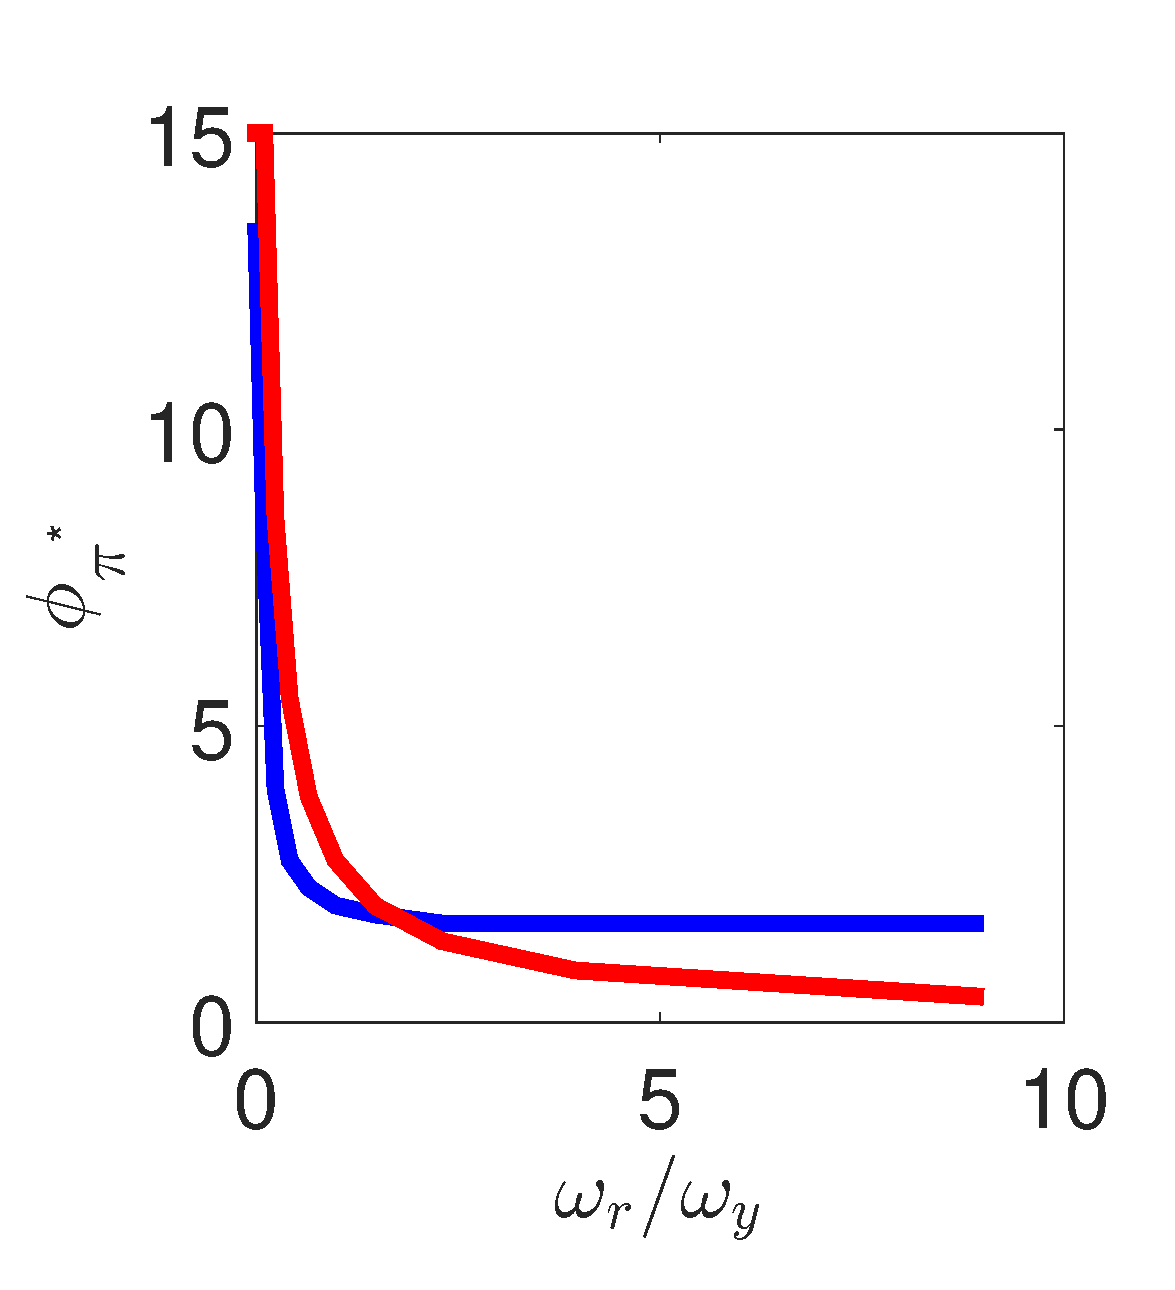
\includegraphics[scale=0.25]{opt_policy_ratios_phiPi.pdf}}} \hspace{5 mm}
      \mbox{\subfigure[$\phi_{y}^{*}$ as a function of  $\frac{\omega_r}{\omega_y}$.]{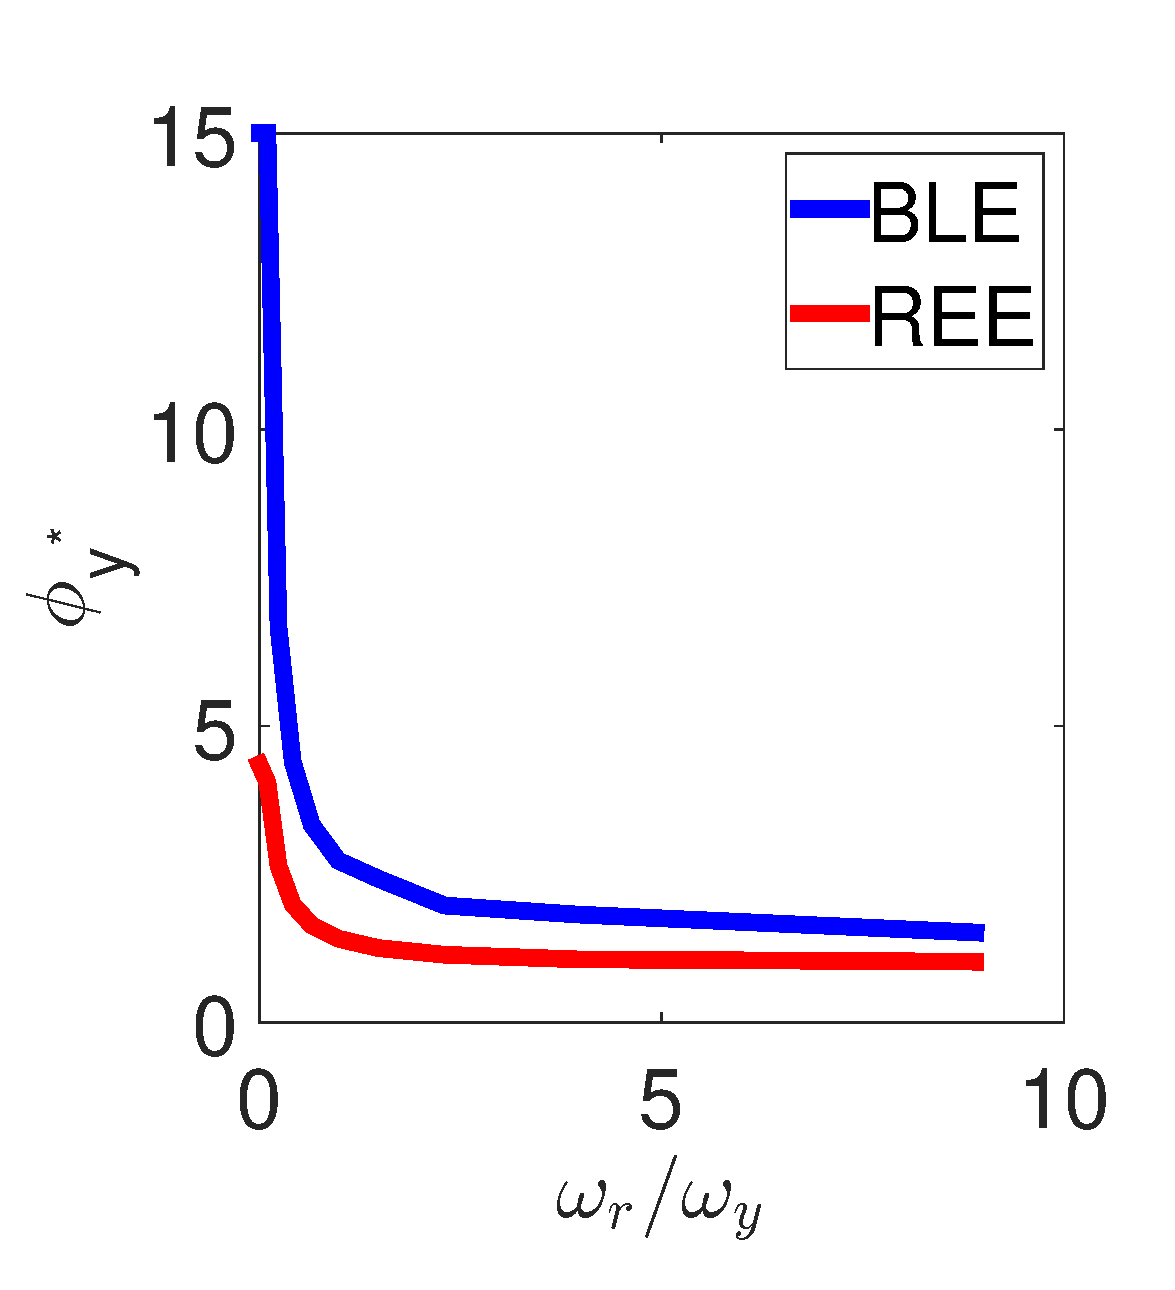
\includegraphics[scale=0.25]{opt_policy_ratios_phiY.pdf}}}\\
      \mbox{\subfigure[IRF of output gap.]{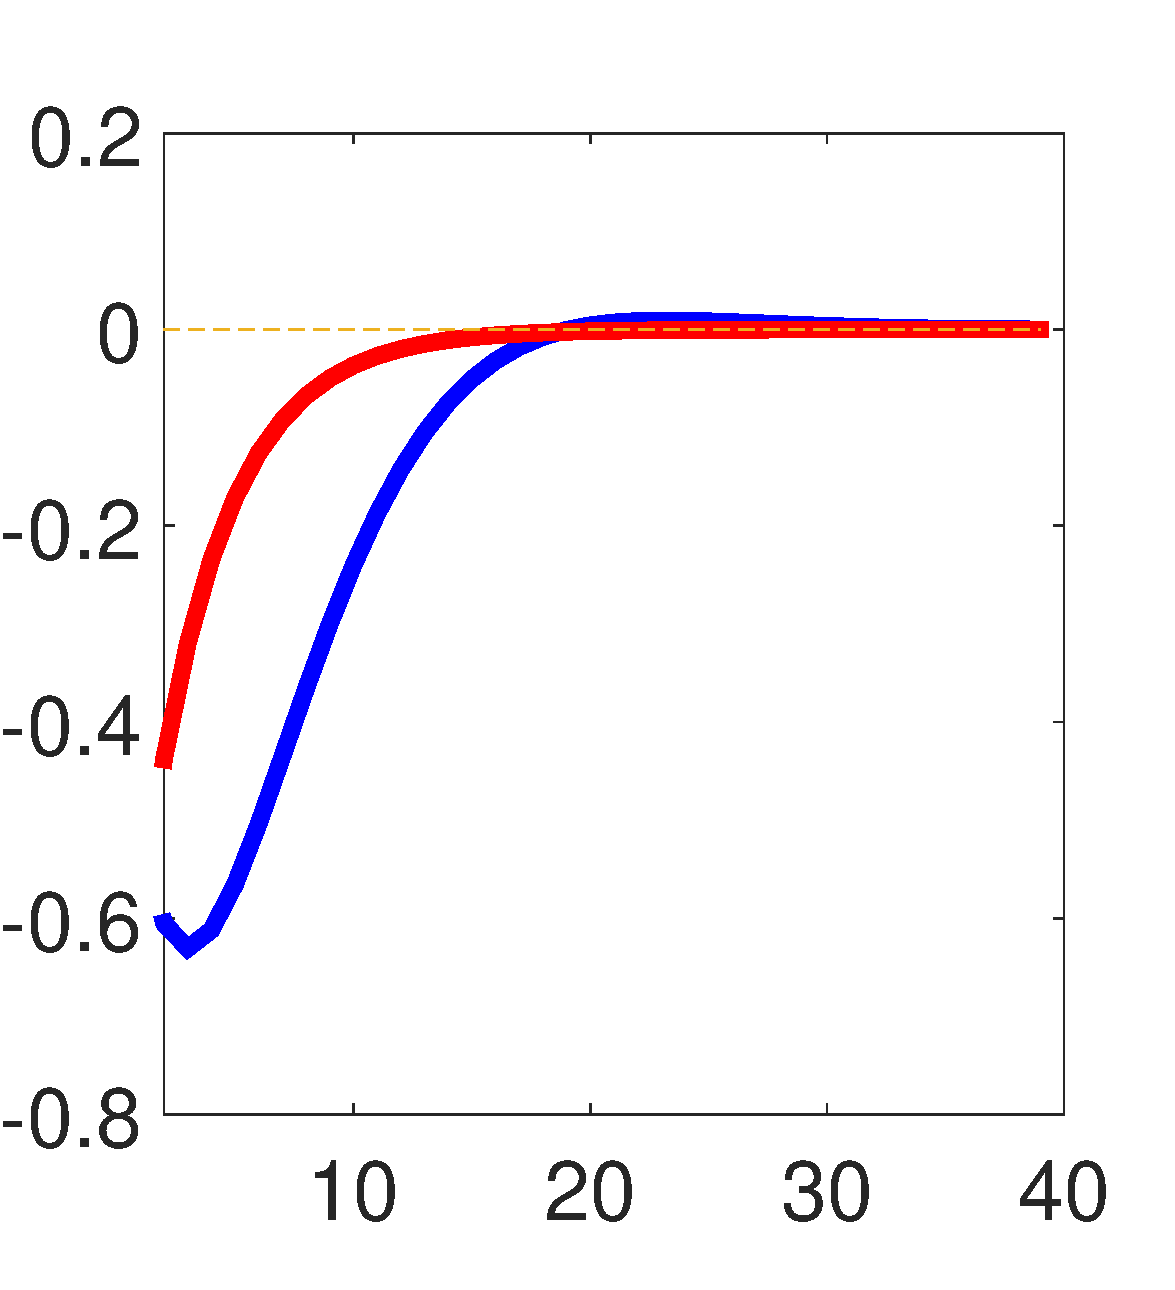
\includegraphics[scale=0.25]{nkpc_irfs_y.pdf} }} \hspace{5 mm}
\mbox{\subfigure[IRF of inflation.]{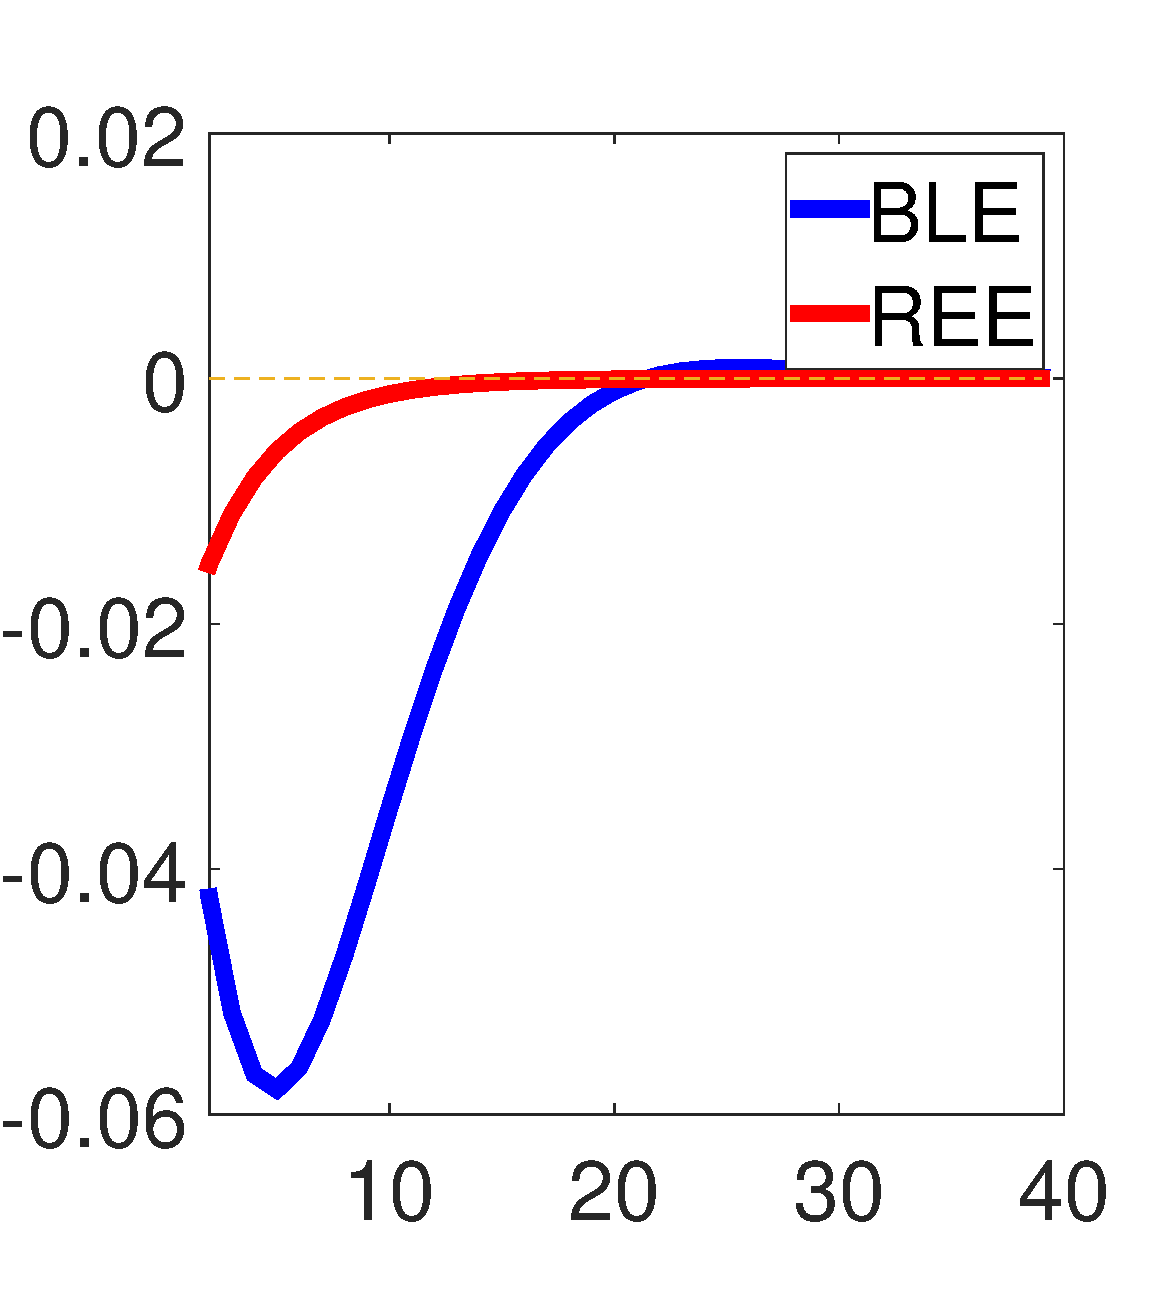
\includegraphics[scale=0.25]{nkpc_irfs_pi.pdf} }}
  \caption{\label{nkpc_irfs} Top panel: changes in optimal parameters as a ratio of weights on interest rates and output gap. Bottom panel: impulse response functions of output gap and inflation to a one standard deviation monetary policy shock.}
    \end{center}
\end{figure}

\vspace{3 mm}


Our analysis so far shows that optimal policy exists under BLE for the calibrated parameters and that the optimal rule $(\phi_{y}^{*},\phi_{\pi}^{*})$ is sensitive to the persistence of exogenous shocks. We next investigate optimal monetary policy for the more empirically relevant case of estimated parameters. In this case the underlying structural parameters are different at BLE and REE, but the variances of inflation, output gap and interest rate are close under these two specifications. In particular, given the estimated parameter values and our benchmark policy weights of $(\omega_y, \omega_r)=(0.1,0.05)$, the expected loss function $E[L]$ is $0.57$ at BLE and $0.55$ at REE\footnote{Our analysis with calibrated parameter values is based on the expressions (\ref{varpic})-(\ref{varrc}). These expressions are no longer applicable for the estimated version of the model since it also includes an interest rate smoothing parameter, and the assumption of same persistence for the exogenous shocks is relaxed. Rather, we use the (different) estimated shock persistence parameters. Therefore we proceed by computing the BLE and the associated variances for each value of policy parameters using the Iterative E-stability algorithm.}. This ensures that the starting point for the loss functions is similar at BLE and REE, unlike the previous case with calibrated parameters.

For this exercise, we limit our attention to Taylor parameters $\phi_y$ and $\phi_{\pi}$ over the range $[0,15]$. Figure \ref{optpolicy_est_figures} shows the optimal rules at BLE and REE for values between $[0, 0.25]$ for $\omega_y$ and $\omega_r$, with $\omega_{\pi}$ fixed at 1. The first result that stands out is, in this case the optimal monetary policy exists not only at BLE, but also at REE for a wide range of policy weights. This difference at REE with estimated parameters arises from the highly persistent shocks and flatter Phillips curve compared with the calibrated parameters, which introduces a larger trade-off between inflation and output gap stabilization, thereby leading to a finite optimal policy for a wide range of policy weights. This additional result allows us to compare how the optimal rules differ under BLE and REE.

Table \ref{optpolicy_est_figures} shows the optimal Taylor rules for several pairs of $(\omega_y,\omega_r)$, along with some key statistics at BLE and REE. The first two rows show our benchmark calibration of $(0.1,0.05)$, while the second row includes a calibration of $(0.048,0.236)$ as in Woodford (1999) and Giannoni (2014). The remaining columns start with the corner case of $(0.25,0)$ with no weight on interest rates, and gradually move to the other corner case of $(0,0.25)$ with no weight on output gap. Several observations stand out from the table: both at BLE and REE, when $\omega_r=0$, there is no optimal policy over the range that we consider\footnote{An optimal policy with larger parameters exists at both BLE and REE if we relax the upper bound of 15. We omit these cases from our discussion here.}. As $\omega_r$ increases, the optimal rules at both BLE and REE decrease to plausible values. An immediate result that stands out is that, $\phi_{\pi}^{*}$ is less sensitive to the policy weights at BLE, while $\phi_y^{*}$ is less sensitive at REE. In other words, optimal monetary policy at REE responds to changes in policy weights mainly through $\phi_{\pi}^{*}$, while optimal monetary policy at BLE responds to these changes through $\phi_y^{*}$. A similar effect can also be seen in Figure \ref{nkpc_irfs}a and \ref{nkpc_irfs}b, which shows the optimal parameters as a function of the ratio of policy weights $\frac{\omega_r}{\omega_y}$. This result is driven by the fact that both estimates of  $\frac{1}{\varphi}$ and $\gamma$ are larger under BLE, which leads to a stronger transmission channel of monetary policy. This in turn allows interest rate changes to have a larger impact on output gap, and a stronger feedback from output gap to inflation at BLE. The stronger transmission channel at BLE is also evident from Figure \ref{nkpc_irfs}c and \ref{nkpc_irfs}d, which shows the impulse responses of inflation and output gap to a monetary policy shock of the same size\footnote{The shock size is one standard deviation at the estimated parameter values for each case, which is the same under BLE and REE with $0.29$.}. Both the initial impact, as well as the cumulative impact of the shock are larger under BLE. Furthermore the shock takes several quarters to reach its full impact under BLE, leading to hump-shaped responses for both inflation and output gap. This is consistent with previous studies in the literature, where a contractionary monetary policy shock typically leads to hump-shaped decreases in output and inflation with peaks after one to two years; see e.g. Leeper et al. (1996) and Christiano et al. (1999). This effect is absent at REE, and it shows that the persistence amplification at BLE is also indirectly reflected in the system's response to an exogenous monetary policy shock. As a consequence of this stronger transmission channel, inflation is more responsive to changes in interest rate at BLE, which leads to smaller fluctuations in $\phi_{\pi}^{*}$. In particular for sufficiently large $\omega_r$, $\phi_{\pi}^{*}$ stabilizes around 1.67 at BLE, which is the close to the standard value of inflation reaction associated with the Taylor rule. Using Woodford (1999) calibration of $(\omega_y,\omega_r)=(0.048,0.236)$, the optimal rule at BLE is given by $(\phi_y^{*},\phi_{\pi}^{*})=(1.67,1.56)$, while the optimal rule at REE falls into the indeterminacy region with $(\phi_y^{*},\phi_{\pi}^{*})=(0.94,0.75)$.

The column $E[L^{*}]$ in Table \ref{optpolicy_est_figures} shows the value of the loss function at the optimal rule for a given pair of weights $(\omega_y,\omega_r)$, and $\Delta E[L^{*}]$ shows the percentage improvement at the optimal rule relative to the loss function at the estimated parameters. It is readily seen that the values for $\Delta E[L^{*}]$ obtained at BLE are generally larger than REE. This is again a consequence of the stronger transmission channel at BLE, which allows monetary policy to have a larger influence in stabilizing the economy. In particular, the optimal variance of inflation obtained at BLE is typically less than half of the optimal variance of inflation at REE. 

In our analysis above, the optimal parameters are inevitably influenced by the degree of interest rate smoothing $\rho_r$. Since this parameter is estimated at different values at BLE and REE with $0.85$ and $0.8$ respectively, we also examine optimal policies at BLE and REE when $\rho_r=0$, which is illustrated at the bottom panel of Table \ref{optpolicy_table}. It is readily seen that our results continue to hold in this case: $\phi_{\pi}^{*}$ is less sensitive and $\phi_y^{*}$ is more sensitive at BLE to changes in policy weights, and the percentage changes $\Delta E[L^{*}]$ in the loss function are generally larger compared to REE. The only difference with the previous case is that the optimal parameters are generally smaller at both BLE and REE, which is expected since shutting off $\rho_r$ allows for larger movements in interest rates, which in turn leads to smaller optimal parameters. This final exercise also reveals that, interest rate smoothing is typically welfare improving at REE, while this is never the case at BLE. $E[L^{*}]$ is uniformly smaller and $ \Delta E[L^{*}]$ uniformly larger at BLE when interest rate smoothing is shut off, while the opposite holds at REE. The result for REE is well-known from Woodford (1999), where a commitment to interest rate smoothing can have a stabilizing effect with forward-looking agents who anticipate and take into account future changes in interest rate. This is different than a BLE with backward-looking agents, where such a commitment does not have a stabilizing effect since agents are unaware of the commitment or do not take it into account when forming their expectations. Overall, these results show that optimal monetary policy at BLE can differ from that at REE in important ways. Particularly, what is optimal under REE may be far from optimal under BLE.




%\begin{figure}
%\centering
%\caption{Impulse responses to a monetary policy shock of one standard deviation. The blue and red lines show the responses under BLE and REE respectively.}
%\label{imp_resp}
%\end{figure}
             
 %We close this section with an illustration of how multiplicity of equilibria can arise under BLE when monetary policy parameters are varied. In all calibration and estimation exercises that we discussed so far, the underlying BLE is unique. However, multiple stable BLE can arise for certain combinations of parameter values. One such case can be observed when we set the parameter values to their CBO-based output gap estimations as given in Table \ref{nkm_alt_gap}, and vary the values of monetary policy parameters. 
%\begin{figure}
%\centering        
%             \mbox{\subfigure[Variances $\sigma_y^2$ and $\sigma_{\pi}^2 $ w.r.t. $\phi_{y}$]{\includegraphics[scale=0.19]{phi_y_variance.pdf}   }} 
% \mbox{\subfigure[Variances $\sigma_y^2$ and $\sigma_{\pi}^2 $ w.r.t. $\phi_{y}$]{\includegraphics[scale=0.19]{phi_pi_variance.pdf}}} \\  
%            \caption{Optimal Policy under BLE and REE at the estimated parameter values.}
%            \label{mult_eqm}
%\end{figure}  
%In this case the estimated Philips curve slope $\gamma$ is smaller at $0.024$ compared with our benchmark estimation with $\gamma=0.035$. Figure \ref{optim_est} illustrates how inflation and output gap variances change as we vary the monetary policy coefficients $\phi_y \in [0.25, 0.5]$ and $\phi_{\pi} \in [1,1.75]$ in this case. While the change in variances follow the same overall pattern as in the benchmark case, we observe two co-existing E-stable BLE over a small range of parameter values. The underlying BLE is unique at the estimated parameter values, but as the reaction coefficients become smaller, with $\phi_y<0.33$ or $\phi_{\pi}<1.3$, another BLE with higher variance and higher persistence for both inflation and output gap becomes stable and there is a range of parameter values where these two stable BLE co-exist. For smaller values of reaction coefficients,
%with $\phi_y < 0.31$ or $\phi_{\pi}<1.1$, 
%the low persistence/low variance equilibrium becomes unstable and only the high-variance equilibrium remains. These results suggest that, for certain parameter combinations, there is another important role for monetary policy in terms of ensuring that such high volatility equilibria are destabilized, which is only possible with a sufficiently active policy rule. In our example multiplicity of equilibria is driven by a flatter Philips curve compared to our benchmark case, but similar results can arise when other structural parameters are varied, such as the exogenous shock persistence parameters $\rho_y$ and $\rho_{\pi}$, or the intertemporal elasticity of substitution $\varphi$. \\




\section{Concluding Remarks}
We have generalized the behavioral learning equilibrium concept to an n-dimensional linear stochastic framework and provided a general iterative method to approximate and estimate BLE.
We have applied our framework to the 3-equation New Keynesian model. Boundedly rational agents use univariate AR(1) forecasting rules for all output gap and inflation. A BLE is parameter free, as along the BLE the two parameters of each rule are pinned down by two observable statistics: the unconditional mean and the first-order
autocorrelation. Hence, to a first-order approximation the simple linear forecasting rule is optimal and consistent with observed market realizations. Agents gradually update the two coefficients --sample mean and
first-order autocorrelation-- of their linear rule through sample autocorrelation learning. In the long run, agents thus learn to coordinate on the best univariate linear forecasting rule for each endogenous state variable, without fully recognizing the more complex structure of the economy.  In higher-dimensional systems, BLE exist under fairly general conditions and we provide simple stability conditions under learning. Coordination on a simple, parsimonious BLE is self-fulfilling and seems a plausible outcome of the coordination process of individual expectations in large complex socio-economic systems.

A striking feature of BLE is the strong {\it persistence amplification}: the persistence of output and inflation along a BLE is much higher, often near unit root, than the persistence in the exogenous shocks driving the economy. Due to these features, estimating the 3-equation model on historical data under BLE yields a substantially better model fit and a different propagation mechanism compared with the REE model.
This leaves an important role for monetary policy with the goal of stabilizing inflation and output.  Different from REE, we find finite optimal Taylor rule coefficients at the BLE in our benchmark calibration. Furthermore, we observe a stronger transmission channel of monetary policy at the estimated parameter values under BLE. A sufficiently aggressive Taylor rule may keep the economy in a stable region with relatively low volatility in inflation and output gap. Future work should study BLE and corresponding optimal policies in more general New Keynesian models.
%We study monetary policies with a Taylor interest rate rule. There are strong direct effects: more aggressive inflation (output) targeting weakens the persistence in inflation (output). Indirect effects may be destabilizing however: more aggressive inflation (output) targeting may lead to more persistent output (inflation). To stabilize both inflation and output, monetary policy must therefore carefully balance between inflation and output targeting. More generally, to check the robustness of policy analysis under RE future work should study policy under more plausible behavioural learning equilibria.

 

\vskip1cm    


\clearpage


%%\subsection{Alternative specifications for setting interest rates}
The monetary policy Taylor rule (\ref{tr}) sets the interest rate in response to contemporaneous output gap $y_t$ and inflation $\pi_t$. This contemporaneous rule assumes that the monetary authority observes current output gap and inflation.  Here we consider two alternative specifications for setting interest rates, widely used in the literature, and perhaps under more realistic informational assumptions of either forward-looking expectations (e.g. through survey data) or observing lagged variables.

\subsubsection{A forward-looking monetary policy rule}
As shown in Bullard and Mitra (2002) and Bullard et al. (2008),
another Taylor-type interest rate rule is to assume that the
monetary authorities set their interest rate instrument in response
to the forecasts of output and inflation deviations. This leads to
the forward expectations specification for the interest rate
equation, where (\ref{tr}) is replaced with
\begin{equation}\label{trexp}
     i_t=\phi_\pi\hat{E}_t\pi_{t+1}+\phi_y \hat{E}_ty_{t+1}.
\end{equation}
Thus the system (\ref{nkmodelm}) becomes
\begin{equation}\label{nkmodelmexp}
    \left\{
    \begin{split}
          {\bf x}_t&={\bf B}\hat{E}_t{\bf x}_{t+1}+{\bf C}\bf{u}_t,\\
          \bf{u}_t&={\pmb\rho}\bf{u}_{t-1}+\pmb{\varepsilon}_t,
    \end{split}
    \right.
\end{equation}
where ${\bf B}=\left[\begin{array}{cc}
1-\varphi\phi_y&\varphi(1-\phi_\pi)\\
\gamma(1-\varphi\phi_y)&\gamma\varphi(1-\phi_\pi)+\lambda
\end{array}\right],\,\,{\bf C}=\left[\begin{array}{cc} 1&0\\
\gamma&1
\end{array}\right].$

Similar to the above contemporaneous data interest rate rules, if the actual law of motion with the PLM in (\ref{xplm}) is stationary, the first-order autocorrelations (\ref{acynk}) and (\ref{acpink}) become\footnote{As in the baseline model above, the first -order sample autocorrelations of output gap and inflation computed based on time series simulationsl are consistent with the complicated expression for $G_{1}$ and $G_{2}$ in Eqs. (\ref{acynkexp}-\ref{acpinkexp}).}
\begin{eqnarray}
G_{1}(\beta_1,\beta_2) &=&\frac{\widetilde{f}_1}{\widetilde{g}_1}\label{acynkexp}\\
G_{2}(\beta_1,\beta_2)
&=&\frac{\widetilde{f}_2}{\widetilde{g}_2}\label{acpinkexp}
\end{eqnarray}
where
\begin{eqnarray*}
\widetilde{f}_1&=&\sigma_1^2\Big\{(\rho+\lambda_1+\lambda_2-\lambda\beta_2^2)[1-\lambda\beta_2^2(\rho+\lambda_1+\lambda_2)]+[\lambda\beta_2^2(\rho\lambda_1+\rho\lambda_2+\lambda_1\lambda_2)-\\
&&\rho\lambda_1\lambda_2][(\rho\lambda_1+\rho\lambda_2+\lambda_1\lambda_2)-\lambda\beta_2^2\rho\lambda_1\lambda_2]\Big\}+\sigma_2^2\Big\{(\varphi(1-\phi_\pi)\beta_2^2)^2[(\rho+\lambda_1+\lambda_2)\\
&&-\rho\lambda_1\lambda_2(\rho\lambda_1+\rho\lambda_2+\lambda_1\lambda_2)]\Big\},\\
\widetilde{g}_1&=&\sigma_1^2\Big\{[(1+\lambda^2\beta_2^4)-2\lambda\beta_2^2(\rho+\lambda_1+\lambda_2)+(1+\lambda^2\beta_2^4)(\rho\lambda_1+\rho\lambda_2+\lambda_1\lambda_2)]\\
&&-\rho\lambda_1\lambda_2[(1+\lambda^2\beta_2^4)(\rho+\lambda_1+\lambda_2)-2\lambda\beta_2^2(\rho\lambda_1+\rho\lambda_2+\lambda_1\lambda_2)+(1+\lambda^2\beta_2^4)\rho\lambda_1\lambda_2]\Big\}\\
&&+\sigma_2^2\Big\{(\varphi(1-\phi_\pi)\beta_2^2)^2[1+\rho\lambda_1+\rho\lambda_2+\lambda_1\lambda_2-\rho\lambda_1\lambda_2(\rho+\lambda_1+\lambda_2)-(\rho\lambda_1\lambda_2)^2]\Big\},\\
\end{eqnarray*}
\begin{eqnarray*}
\widetilde{f}_2&=&\sigma_1^2\Big\{\gamma^2[(\rho+\lambda_1+\lambda_2)-\rho\lambda_1\lambda_2(\rho\lambda_1+\rho\lambda_2+\lambda_1\lambda_2)]\Big\}+\sigma_2^2\Big\{[(\rho+\lambda_1+\lambda_2)-(1-\varphi\phi_y)\beta_1^2]\cdot\\
&&[1-(1-\varphi\phi_y)\beta_1^2(\rho+\lambda_1+\lambda_2)]+[(1-\varphi\phi_y)\beta_1^2(\rho\lambda_1+\rho\lambda_2+\lambda_1\lambda_2)-\rho\lambda_1\lambda_2]\cdot\\
&&[(\rho\lambda_1+\rho\lambda_2+\lambda_1\lambda_2)-(1-\varphi\phi_y)\beta_1^2\rho\lambda_1\lambda_2]\Big\},\\
\widetilde{g}_2&=&\sigma_1^2\Big\{\gamma^2[1+\rho\lambda_1+\rho\lambda_2+\lambda_1\lambda_2-\rho\lambda_1\lambda_2(\rho+\lambda_1+\lambda_2)-(\rho\lambda_1\lambda_2)^2]\Big\}\\
&&+\sigma_2^2\Big\{[1+((1-\varphi\phi_y)\beta_1^2)^2-2(1-\varphi\phi_y)\beta_1^2(\rho+\lambda_1+\lambda_2)+(1+((1-\varphi\phi_y)\beta_1^2)^2)\cdot\\
&&(\rho\lambda_1+\rho\lambda_2+\lambda_1\lambda_2)]-\rho\lambda_1\lambda_2[(1+((1-\varphi\phi_y)\beta_1^2)^2)(\rho+\lambda_1+\lambda_2)-2(1-\varphi\phi_y)\beta_1^2\cdot\\
&&(\rho\lambda_1+\rho\lambda_2+\lambda_1\lambda_2)+(1+((1-\varphi\phi_y)\beta_1^2)^2)\rho\lambda_1\lambda_2]\Big\},
\end{eqnarray*}
\begin{eqnarray*}
\lambda_1+\lambda_2&=&(1-\varphi\phi_y)\beta_1^2+(\gamma\varphi(1-\phi_\pi)+\lambda)\beta_2^2,\\
\lambda_1\lambda_2&=&\lambda(1-\varphi\phi_y)\beta_1^2\beta_2^2.
\end{eqnarray*}
In this case we have some similar results on the existence and stability as in the baseline model. Since the coefficients matrices are different, the corresponding sufficient conditions change.
\begin{cor}
\label{cor:exp} Under the forward-looking interest rate rule, if $\phi_y<\frac{1}{\varphi}$ and $1<\phi_\pi<1+\frac{\lambda}{\gamma\varphi}$, then there
exists at least one BLE $(\pmb\alpha^*,\pmb\beta^*)$, where
$\pmb\alpha^*=\bf 0=\overline{\bf x^*}$. Furthermore, the BLE $(\pmb\alpha^*,{\pmb\beta}^*)$ is locally
stable under SAC-learning if all the eigenvalues of $\pmb D\pmb G_{\pmb\beta}(\pmb\beta^*)=\Big(\frac{\partial G_i}{\partial \beta_j}\Big)_{{\pmb\beta}={\pmb\beta}^*}$ have real parts less than 1.
\end{cor}
\textbf{Proof.} See Appendix \ref{corfor}.

\begin{figure}
    \begin{center}
        \mbox{\subfigure[]
        {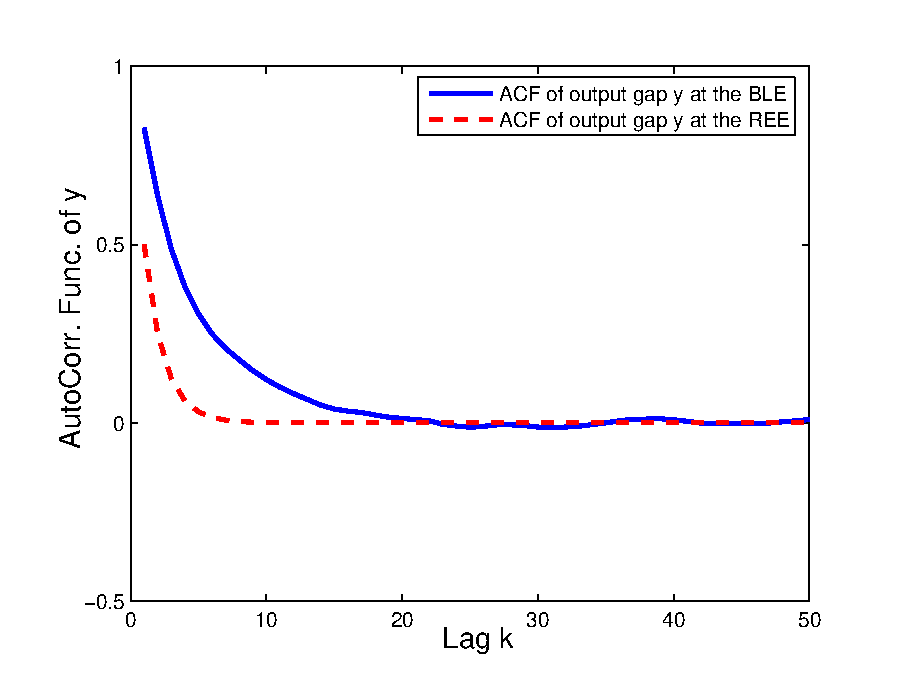
\includegraphics[width=3in]{acfytrexp2.eps}}\quad
        \subfigure[]
         {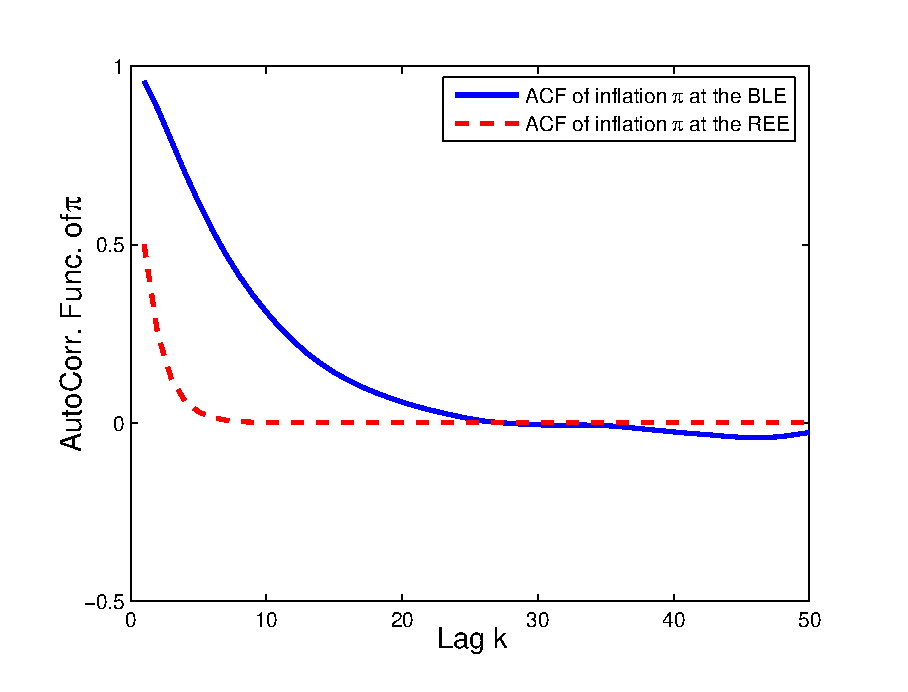
\includegraphics[width=3in]{acfpitrexp2.eps}}}
   \end{center}
   \caption{\label{aftrexp} Autocorrelation functions of output gap $y$ and inflation $\pi$ with forward-looking Taylor rule at the BLE $(\beta_1^*,
   \beta_2^*)=(0.8326, 0.9605)$. Parameters are: $\lambda=0.99, \varphi=1, \gamma=0.04, \rho=0.5, \phi_\pi=1.5,\phi_y=0.5, \sigma_{2}/\sigma_1=0.5$. }
    \end{figure}



\begin{figure}
    \begin{center}
        \mbox{\subfigure[]
        {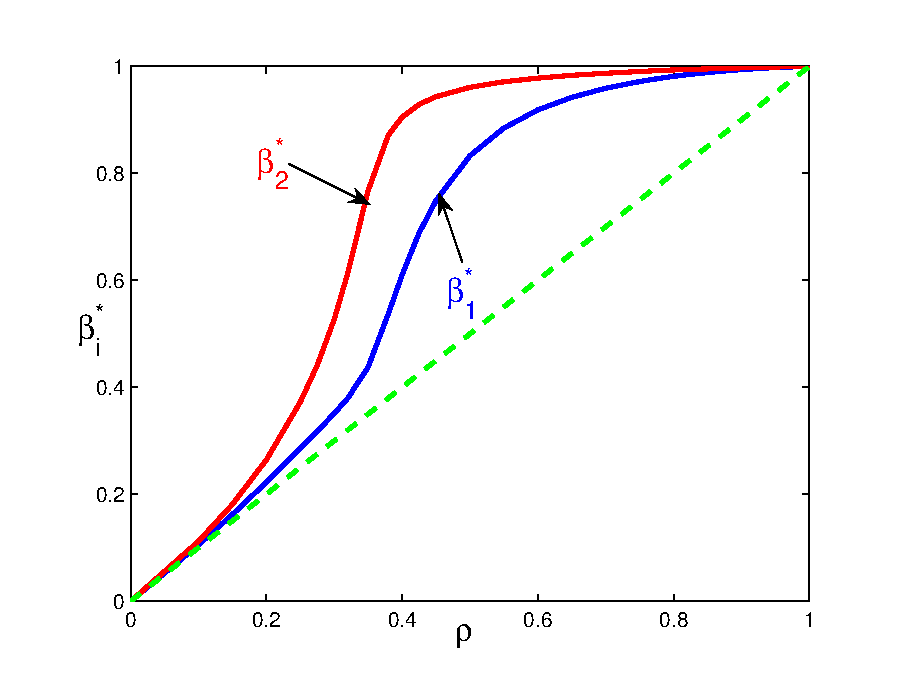
\includegraphics[width=3in]{blerhotrexp.eps}}
        \subfigure[]
         {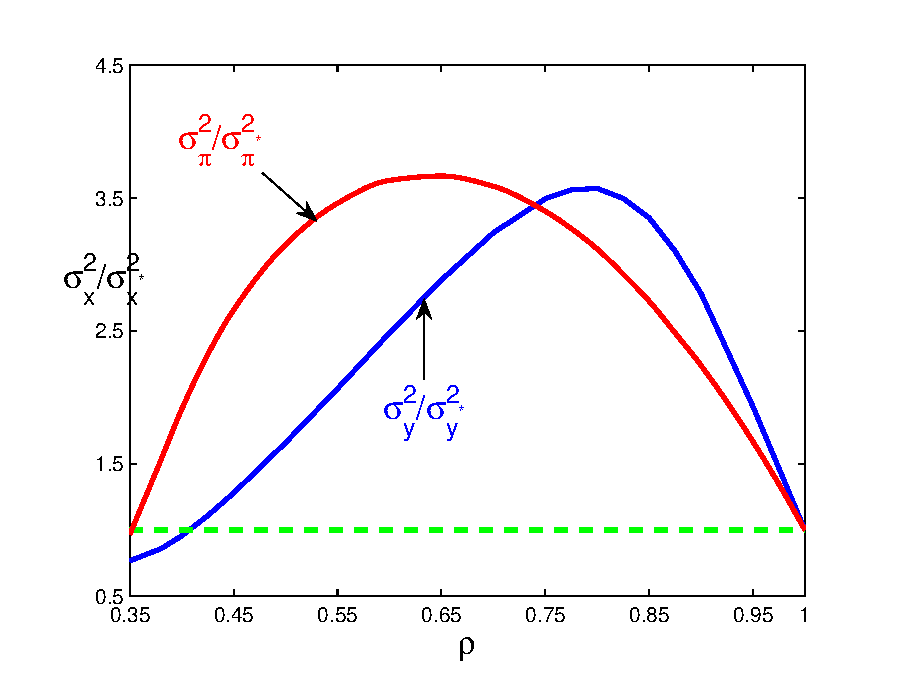
\includegraphics[width=3in]{varrhotrexp.eps}}}
   \end{center}
   \caption{ \label{blerhotrexp}
   BLE $(\beta^*_1, \beta^*_2)$ as a function of the persistence $\rho$ of the exogenous shocks with forward-looking Taylor rule (a) $\beta^*_i (i=1,2)$ with respect to $\rho$;  (b) the ratio of variances ($\sigma_y^2/\sigma_{y^*}^2$, $\sigma_\pi^2/\sigma_{\pi^*}^2$) with respect to $\rho$ at the corresponding BLE $(\beta^*_1, \beta^*_2)$. Parameters are: $\lambda=0.99, \varphi=1, \gamma=0.04, \phi_\pi=1.5,\phi_y=0.5, \frac{\sigma_2}{\sigma_1}=0.5$.  }
    \end{figure}

For the same benchmark parameter values as in the contemporaneous Taylor rule, the system has a BLE $(\beta_1^*,\beta_2^*)=(0.8326, 0.9605)$, with output and inflation much more persistent than the REE benchmark (with $\rho=0.5$), as illustrated in Figure \ref{aftrexp}. Figure \ref{blerhotrexp}a illustrates how these results depend on the parameter $\rho$, the persistence of the exogenous shocks. As before, for the forward looking Taylor rule, the system also displays {\it persistence amplification}, with the persistence of inflation and output gap along BLE much higher than the persistence $\rho$ of the exogenous shocks. Similarly, Figure \ref{blerhotrexp}b illustrates the excess volatility of inflation and output compared to the REE benchmark.

%Interestingly, we find multiple BLE here with proper parameters. For example, if we consider different parameters of $\phi_y$ and $\phi_\pi$ with $\phi_y=8$, $\phi_\pi=6$ and the other parameters given as in the benchmark case, we find three BLE $(\beta_1^*, \beta_2^*)=(0.9922,0.9664), (0.3203,0.8727), (-0.351, 0.8637)$, as shown in Figure \ref{BLEm_trexp}.

Here we also find finite optimal coefficients as for the contemporaneous Taylor rule. The difference is that here the optimal policy is $(\phi_y^*, \phi_\pi^*)=(1.1793,10.7942)$, which are both higher than in the contemporaneous case. We further study how the finite optimal coefficients respond as the persistence $\rho$ of shocks and the weight $\omega$ on inflation change. Figure \ref{optrhotrexp}a indicates that the finite optimal $\phi_\pi^*$ increases as $\rho$ varies around $0.5$, while $\phi_y^*$ changes only a little. This is because in this case the ratio $\sigma_\pi^2/\sigma_y^2$  of variances of inflation and output gap is relatively larger than in the contemporaneous case. For example, given the benchmark parameters, the variances of output gap and inflation at the BLE are $3.963$ and $4.097$ while they are $3.855$ and $3.595$, respectively, in the contemporaneous case. So here the variance of inflation plays a more important role and the finite optimal policy $\phi_\pi^*$ changes faster than $\phi_y^*$. Figure \ref{optomegatrexp} suggests similar effects of the weight of inflation $\omega$ on the finite optimal coefficients and optimal manifolds. Similar to the contemporaneous case, the optimal manifold moves up generally as $\rho$ or $\omega$ grows. In addition, Figure  \ref{optomegatrexp}b suggests that, as before, $\phi_\pi^*\approx 1.5$, if $\phi_y^*=0.5$ in the optimal manifold for $\omega=0.5$ in the framework of BLE and the loss function decreases very slowly till the finite optimal policy after $\phi_y^*=0.5$, as shown in Figure \ref{lossfopt_trexp}.

 \begin{figure}
    \begin{center}
       % \mbox{\subfigure[Effects of $\phi_{\pi}$ and $\phi_y$ on $\beta_1^*$]
%        {\includegraphics[width=3in]{blebeta1phipiC1.eps}}\quad
%        \subfigure[Effects of $\phi_{\pi}$ and $\phi_y$ on $\beta_2^*$]
%         {\includegraphics[width=3in]{blebeta2phipiC1.eps}}}
          \mbox{\subfigure[Optimal policy]
        {\includegraphics[width=3in]{optpolicyrho_trexp.eps}}\quad
        \subfigure[Optimal manifold]
         {\includegraphics[width=3in]{optmanifrho_trexp.eps}}}
        \end{center}
   \caption{ \label{optrhotrexp}
   Optimal policies at the BLE with respect to $\rho$ (a) and corresponding optimal manifolds for three different $\rho$ (connection points of solid and dotted curves corresponding to finite optimal policies) (b) with the forward-looking interest rate rule. Parameters are: $\lambda=0.99, \varphi=1, \gamma=0.04,\frac{\sigma_2}{\sigma_1}=0.5$ and $\omega=0.9$. }
    \end{figure}
    
    \begin{figure}
    \begin{center}
       % \mbox{\subfigure[Effects of $\phi_{\pi}$ and $\phi_y$ on $\beta_1^*$]
%        {\includegraphics[width=3in]{blebeta1phipiC1.eps}}\quad
%        \subfigure[Effects of $\phi_{\pi}$ and $\phi_y$ on $\beta_2^*$]
%         {\includegraphics[width=3in]{blebeta2phipiC1.eps}}}
          \mbox{\subfigure[Optimal policy]
        {\includegraphics[width=3in]{optpolicyomega_trexp.eps}}\quad
        \subfigure[Optimal manifold]
         {\includegraphics[width=3in]{optmanifomega_trexp.eps}}}
        \end{center}
   \caption{ \label{optomegatrexp}
  Optimal policies at the BLE with respect to $\omega$ (a) and corresponding optimal manifolds for three different $\omega$ (connection points of solid and dotted curves corresponding to finite optimal policies) (b) with the forward-looking interest rate rule.
   Parameters are: $\lambda=0.99, \varphi=1, \gamma=0.04, \sigma_{2}/\sigma_1=0.5$ and $\rho=0.5$. }
    \end{figure}
    
    \begin{figure}
    \begin{center}
        \mbox{\subfigure[]
        {\includegraphics[width=3.2in]{optimalvar_trexp2.eps}}\quad
        \subfigure[]
         {\includegraphics[width=3.2in]{optimalvar_trexp1.eps}}}
   \end{center}
   \caption{\label{lossfopt_trexp} Loss function along the optimal manifold in Figure \ref{optomegatrexp}(b) with $\omega=0.5$ for different ranges of $\phi_y^*$, i.e. $\phi_y^*\in [0, 2]$ (a) and  $\phi_y^*\in[1.5, 2]$ (b). Parameters are: $\lambda=0.99, \varphi=1, \gamma=0.04, \rho=0.5,
\frac{\sigma_2}{\sigma_1}=0.5$ and $\omega=0.5$.}
    \end{figure}
    
    \pagebreak

\subsubsection{A lagged monetary policy rule}
As argued e.g. in Bullard and Mitra (2002), it may be viewed as realistic for central bank practice to posit that the monetary authorities must react to last quarter's observations on
inflation and output gap as contemporaneous values are not known yet. This leads to the lagged data specification for the interest rate equation, where (\ref{tr}) is
replaced by
\begin{equation}\label{trlag}
     i_t=\phi_\pi\pi_{t-1}+\phi_y y_{t-1}.
\end{equation}
Due to the lagged monetary policy rule the system (\ref{nkmodelm}) includes an additional lagged term $x_{t-1}$ and becomes

\begin{equation}\label{nkmodelmlag}
    \left\{
    \begin{split}
          {\pmb x}_t&={\pmb A} {\pmb x}_{t-1}+{\pmb B} {\pmb x}_{t+1}^e+{\pmb C}\pmb{u}_t,\\
          \pmb{u}_t&={\pmb\rho}\pmb{u}_{t-1}+\pmb{\varepsilon}_t,
    \end{split}
    \right.
\end{equation}
where ${\pmb A}=\left[\begin{array}{cc}
-\varphi\phi_y&-\varphi\phi_\pi\\
-\gamma\varphi\phi_y&-\gamma\varphi\phi_\pi
\end{array}\right],\,\,{\pmb B}=\left[\begin{array}{cc}
1&\varphi\\
\gamma&\gamma\varphi+\lambda
\end{array}\right],\,\,{\pmb C}=\left[\begin{array}{cc} 1&0\\
\gamma&1
\end{array}\right].$

Similar to the above two interest rate rules, if the actual law of motion with the PLM in (\ref{xplm}) is stationary, %Besides the condition of existence and stability of BLE, the difference from the baseline model just lies in the expression of the first-order autocorrelations. In the case of the lagged rule, following similar calculations as in  the baseline model,
the first-order autocorrelations (\ref{acynk}) and (\ref{acpink})
become
%\footnote{As in the baseline line, the first-order autocorrelations of output gap and inflation calculated based on the time series generated by the model using the statistical definition of autocorrelation are consistent with those calculated based on the following equations. Hence although the expressions of $G_{1}$ and $G_{2}$ are extremely complicated, it can be sure that they are correct.}
\begin{eqnarray}
G_{1}(\beta_1,\beta_2) &=&\frac{\widetilde{f}_1}{\widetilde{g}_1}\label{acynklag}\\
G_{2}(\beta_1,\beta_2)
&=&\frac{\widetilde{f}_2}{\widetilde{g}_2}\label{acpinklag}
\end{eqnarray}
where
\begin{eqnarray*}
\widetilde{f}_1&=&\sigma_1^2\Big\{(\rho+\lambda_1+\lambda_2-\lambda\beta_2^2)[1-\lambda\beta_2^2(\rho+\lambda_1+\lambda_2)]+[\lambda\beta_2^2(\rho\lambda_1+\rho\lambda_2+\lambda_1\lambda_2)-\\
&&\rho\lambda_1\lambda_2][(\rho\lambda_1+\rho\lambda_2+\lambda_1\lambda_2)-\lambda\beta_2^2\rho\lambda_1\lambda_2]\Big\}+\sigma_2^2\Big\{(\varphi\phi_\pi-\varphi\beta_2^2)^2[(\rho+\lambda_1+\lambda_2)\\
&&-\rho\lambda_1\lambda_2(\rho\lambda_1+\rho\lambda_2+\lambda_1\lambda_2)]\Big\},\\
\widetilde{g}_1&=&\sigma_1^2\Big\{[(1+\lambda^2\beta_2^4)-2\lambda\beta_2^2(\rho+\lambda_1+\lambda_2)+(1+\lambda^2\beta_2^4)(\rho\lambda_1+\rho\lambda_2+\lambda_1\lambda_2)]\\
&&-\rho\lambda_1\lambda_2[(1+\lambda^2\beta_2^4)(\rho+\lambda_1+\lambda_2)-2\lambda\beta_2^2(\rho\lambda_1+\rho\lambda_2+\lambda_1\lambda_2)+(1+\lambda^2\beta_2^4)\rho\lambda_1\lambda_2]\Big\}\\
&&+\sigma_2^2\Big\{(\varphi\phi_\pi-\varphi\beta_2^2)^2[1+\rho\lambda_1+\rho\lambda_2+\lambda_1\lambda_2-\rho\lambda_1\lambda_2(\rho+\lambda_1+\lambda_2)-(\rho\lambda_1\lambda_2)^2]\Big\},\\
\end{eqnarray*}
\begin{eqnarray*}
\widetilde{f}_2&=&\sigma_1^2\Big\{\gamma^2[(\rho+\lambda_1+\lambda_2)-\rho\lambda_1\lambda_2(\rho\lambda_1+\rho\lambda_2+\lambda_1\lambda_2)]\Big\}+\sigma_2^2\Big\{[(\rho+\lambda_1+\lambda_2)-(\beta_1^2-\varphi\phi_y)]\cdot\\
&&[1-(\beta_1^2-\varphi\phi_y)(\rho+\lambda_1+\lambda_2)]+[(\beta_1^2-\varphi\phi_y)(\rho\lambda_1+\rho\lambda_2+\lambda_1\lambda_2)-\rho\lambda_1\lambda_2]\cdot\\
&&[(\rho\lambda_1+\rho\lambda_2+\lambda_1\lambda_2)-(\beta_1^2-\varphi\phi_y)\rho\lambda_1\lambda_2]\Big\},\\
\widetilde{g}_2&=&\sigma_1^2\Big\{\gamma^2[1+\rho\lambda_1+\rho\lambda_2+\lambda_1\lambda_2-\rho\lambda_1\lambda_2(\rho+\lambda_1+\lambda_2)-(\rho\lambda_1\lambda_2)^2]\Big\}\\
&&+\sigma_2^2\Big\{[(1+(\beta_1^2-\varphi\phi_y)^2)-2(\beta_1^2-\varphi\phi_y)(\rho+\lambda_1+\lambda_2)+(1+(\beta_1^2-\varphi\phi_y)^2)\cdot\\
&&(\rho\lambda_1+\rho\lambda_2+\lambda_1\lambda_2)]-\rho\lambda_1\lambda_2[(1+(\beta_1^2-\varphi\phi_y)^2)(\rho+\lambda_1+\lambda_2)-2(\beta_1^2-\varphi\phi_y)\cdot\\
&&(\rho\lambda_1+\rho\lambda_2+\lambda_1\lambda_2)+(1+(\beta_1^2-\varphi\phi_y)^2)\rho\lambda_1\lambda_2]\Big\},
\end{eqnarray*}
\begin{eqnarray*}
\lambda_1+\lambda_2&=&\beta_1^2-\varphi\phi_y-\gamma\varphi\phi_\pi+(\gamma\varphi+\lambda)\beta_2^2,\\
\lambda_1\lambda_2&=&\lambda(\beta_1^2-\varphi\phi_y)\beta_2^2.
\end{eqnarray*}

Note that, because of the additional lagged term $x_{t-1}$, the rational expectations equilibrium is different compared to the system without this lagged term ${\pmb x}_{t-1}$ in the previous two cases. The proofs concerning existence and stability of BLE, however, are straightforward extensions of the proofs without the additional term ${\pmb x}_{t-1}$\footnote{In particular, the system (\ref{nkmodelmlag}) can be rewritten in the form of Eq. (\ref{modeln30}) in appendix \ref{acfnkc}, when BLE is considered. The difference from the baseline case lies in different coefficient matrices $ {\bf z}_{t}=\pmb{(A+B\beta^2)}{\bf z}_{t-1}+\pmb{C\varepsilon}_t+\pmb{C\rho I \varepsilon}_{t-1}+\cdots$ with matrices ${\bf A, B, C}$ as in the system (\ref{nkmodelmlag}). Then following the same idea of the proof, the first-order autocorrelations for the lagged monetary policy rule in (\ref{acynklag}) and (\ref{acpinklag}) are obtained. Similar proofs of propositions 1 and 2, concerning existence and stability of BLE, can then be obtained.}. In this case we have similar results on the existence and stability on BLE as in the baseline model.
\begin{cor}
\label{cor:lag} Under the lagged interest rate rule, if $\phi_y<\frac{1}{\varphi}$ and $1<\phi_\pi<\frac{1-\varphi\phi_y}{\gamma\varphi}$, then there
exists at least one BLE $(\pmb\alpha^*,\pmb\beta^*)$. Furthermore, the BLE $(\pmb\alpha^*,{\pmb\beta}^*)$ is locally
stable under SAC-learning if all the eigenvalues of $\pmb D\pmb G_{\pmb\beta}(\pmb\beta^*)=\Big(\frac{\partial G_i}{\partial \beta_j}\Big)_{{\pmb\beta}={\pmb\beta}^*}$ have real parts less than 1.
\end{cor}
\textbf{Proof.} See Appendix \ref{corlagproof}.

\begin{figure}
    \begin{center}
        \mbox{\subfigure[ ]
        {\includegraphics[width=3in]{acfytrlag2.eps}}\quad
        \subfigure[]
         {\includegraphics[width=3in]{acfpitrlag2.eps}}}
   \end{center}
   \caption{\label{aftrlag} Autocorrelation functions of output gap $y$ and inflation $\pi$ with lagged Taylor rule at the BLE $(\beta_1^*,
   \beta_2^*)=(0.7746, 0.9628)$. Parameters are: $\lambda=0.99, \varphi=1, \gamma=0.04, \rho=0.5, \phi_\pi=1.5,\phi_y=0.5, \sigma_{2}/\sigma_1=0.5$.}
    \end{figure}
    
    \begin{figure}
    \begin{center}
    \includegraphics[width=4in]{blerhotrlag.eps}
       % %\mbox{\subfigure[]
%        {\includegraphics[width=3in]{blerhotrlag.eps}}\quad
%        %\subfigure[]
%%         {\includegraphics[width=3in]{varrhotrc.eps}}
%}
   \end{center}
   \caption{ \label{blerhotrlag} Effects of $\rho$ with lagged Taylor rule, i.e. $\beta^*_i (i=1,2)$ with respect to $\rho$. Parameters are: $\lambda=0.99, \varphi=1, \gamma=0.04, \phi_\pi=1.5,\phi_y=0.5, \frac{\sigma_2}{\sigma_1}=0.5$. }
    \end{figure}

For the same benchmark parameter values as before, the system has a BLE $(\beta_1^*,\beta_2^*)=(0.7746, 0.9628)$. Figure \ref{aftrlag} illustrates the ACF of output and inflation along the BLE and shows that they are much more persistent than the autocorrelations in the exogenous shocks. Figure \ref{blerhotrlag} illustrates that the model with a lagged Taylor rule also exhibits {\it persistence amplification} within the empirically relevant region of parameters $\rho\geq 0.5$ (cf. footnote\ref{note:emprel}).
% Interestingly, we find multiple BLE here with proper parameters. For example, if we consider different parameters of $\phi_y$ and $\phi_\pi$ with $\phi_y=0.8$, $\phi_\pi=1.85$ and the other parameters given as in the benchmark case, we find three BLE $(\beta_1^*, \beta_2^*)=(0.5848, 0.9626), (0.3992,0.9659), (0.1182,0.9678)$, as shown in Figure \ref{BLEm_trlag}.


Here we find finite optimal coefficients again as in the contemporaneous and forward-looking Taylor rules. The difference is that here the optimal policy is $(\phi_y^*, \phi_\pi^*)=(0.4566, 5.2008)$. We further study how the finite optimal coefficients respond as the persistence $\rho$ of shocks and the weight on inflation $\omega$ change. Figure \ref{optrhotrlag}a indicates that finite optimal $\phi_\pi^*$ increases as $\rho$ varies around $0.5$ while $\phi_y^*$ changes just a little, similar to the forward-looking case. This is also because in this case the ratio of variances of inflation and output gap is also larger than in the contemporaneous case, that is, the variance of inflation plays a more dominant role.  For example, given the benchmark parameters, the variances of output gap and inflation at the BLE are $3.145$ and $4.310$, while they are $3.855$ and $3.595$, respectively, in the contemporaneous case. Therefore, similar to the forward-looking case, the finite optimal policy $\phi_\pi^*$  changes faster than $\phi_y^*$. Figure \ref{optomegatrlag} suggests similar effects of the weight on inflation $\omega$ on the finite optimal coefficients and optimal manifolds. In addition, if we consider $\omega=0.5$, Figure \ref{lossfopt_trlag} suggests that, as before, $(\phi_y^*,\phi_\pi^*)=(0.5, 1.5)$ is nearly optimal in the case the weight $\omega=0.5$.

\begin{figure}
    \begin{center}
       % \mbox{\subfigure[Effects of $\phi_{\pi}$ and $\phi_y$ on $\beta_1^*$]
%        {\includegraphics[width=3in]{blebeta1phipiC1.eps}}\quad
%        \subfigure[Effects of $\phi_{\pi}$ and $\phi_y$ on $\beta_2^*$]
%         {\includegraphics[width=3in]{blebeta2phipiC1.eps}}}
          \mbox{\subfigure[Optimal policy]
        {\includegraphics[width=3in]{optpolicyrho_trlag.eps}}\quad
        \subfigure[Optimal manifold]
         {\includegraphics[width=3in]{optmanifrho_trlag.eps}}}
        \end{center}
   \caption{ \label{optrhotrlag}
  Optimal policies at the BLE with respect to $\rho$ (a) and corresponding optimal manifolds for three different $\rho$ (connection points of solid and dotted curves corresponding to finite optimal policies) (b) with the lagged interest rate rule.
   Parameters are: $\lambda=0.99, \varphi=1, \gamma=0.04, \sigma_{2}/\sigma_1=0.5$ and $\omega=0.9$. }
    \end{figure}
    
\begin{figure}
    \begin{center}
       % \mbox{\subfigure[Effects of $\phi_{\pi}$ and $\phi_y$ on $\beta_1^*$]
%        {\includegraphics[width=3in]{blebeta1phipiC1.eps}}\quad
%        \subfigure[Effects of $\phi_{\pi}$ and $\phi_y$ on $\beta_2^*$]
%         {\includegraphics[width=3in]{blebeta2phipiC1.eps}}}
          \mbox{\subfigure[Optimal policy]
        {\includegraphics[width=3in]{optpolicyomega_trlag.eps}}\quad
        \subfigure[Optimal manifold]
         {\includegraphics[width=3in]{optmanifomega_trlag.eps}}}
        \end{center}
   \caption{ \label{optomegatrlag}
  Optimal policies at the BLE with respect to $\omega$ (a) and corresponding optimal manifolds for three different $\omega$ (connection points of solid and dotted curves corresponding to finite optimal policies) (b) with the lagged interest rate rule.
   Parameters are: $\lambda=0.99, \varphi=1, \gamma=0.04,\sigma_{2}/\sigma_1=0.5$ and $\rho=0.5$. }
    \end{figure}    
    
 \begin{figure}
    \begin{center}
        \mbox{\subfigure[Optimal manifold]
        {\includegraphics[width=3in]{optmanifomega05_trlag.eps}}\quad
        \subfigure[Loss function]
         {\includegraphics[width=3in]{varoptpolicyomega05_trlag.eps}}}
        \end{center}
   \caption{ \label{lossfopt_trlag}
  Optimal manifold at the BLE for $\omega=0.5$ (connection points of solid and dotted curves corresponding to finite optimal policies) (a) and corresponding loss function along the optimal manifold(b) with the lagged interest rate rule.
   Parameters are: $\lambda=0.99, \varphi=1, \gamma=0.04, \rho=0.5, \sigma_{2}/\sigma_1=0.5$, $\omega=0.5$. }
    \end{figure}   \\
\section*{Appendix}
\begin{appendix}

\section{Mean of the rational expectations equilibrium}
\label{appA}
Using (\ref{xf1}-\ref{div2}) and  (\ref{reec0}-\ref{reec3}) the mean satisfies
 \begin{eqnarray*}
 \overline{\bf x^*}&=&({\pmb I}-{\pmb c}_1)^{-1}(\pmb{c}_0+{\pmb c}_2\overline {\pmb u})\\
 &=&({\pmb I}-{\pmb c}_1)^{-1}({\pmb I}-{\pmb b}_1{\pmb c}_1-{\pmb b}_1)^{-1}({\pmb b}_0+{\pmb b}_1{\pmb c}_2{\pmb a})+({\pmb I}-{\pmb c}_1)^{-1}{\pmb c}_2({\pmb I}-{\pmb\rho})^{-1}{\pmb a}\\
 &=&({\pmb I}-{\pmb c}_1)^{-1}({\pmb I}-{\pmb b}_1{\pmb c}_1-{\pmb b}_1)^{-1}[{\pmb b}_0+({\pmb b}_1{\pmb c}_2({\pmb I}-{\pmb\rho})+({\pmb I}-{\pmb b}_1{\pmb c}_1-{\pmb b}_1){\pmb c}_2)({\pmb I}-{\pmb\rho})^{-1}{\pmb a}]\\
 &=&[({\pmb I}-{\pmb b}_1{\pmb c}_1-{\pmb b}_1)({\pmb I}-{\pmb c}_1)]^{-1}[{\pmb b}_0+{\pmb b}_3({\pmb I}-{\pmb\rho})^{-1}{\pmb a}]\\
  &=&({\pmb I}-{\pmb b}_1-{\pmb b}_2)^{-1}[{\pmb b}_0+{\pmb b}_3({\pmb I}-{\pmb\rho})^{-1}{\pmb a}].
\end{eqnarray*}


\section{Autocorrelation in the $n$-dimensional case}\label{ACFn}
The purpose of this appendix is to show that the first-order autocorrelation coefficients of the stochastic stationary system (\ref{xfalm}) are continuous functions with respect to $(\beta_1, \beta_2, \cdots,\beta_n)$ and the other related parameters. Rewrite model (\ref{xfalm}) as
\begin{equation}\label{modelmpn1}
    \left\{
    \begin{split}
            {\pmb x}_{t}-{\pmb{\overline x}}&=({\pmb b}_1 {\pmb\beta}^2+{\pmb b}_2)({\pmb x}_{t-1}-{\pmb{ \overline x}})+{\pmb b}_3({\pmb u}_t-{\pmb{ \overline u}})+{\pmb b}_4{\pmb v}_t,\\
            {\pmb u}_{t}-{\pmb {\overline u}}&={\pmb\rho} ({\pmb u}_{t-1}-{\pmb{\overline u}})+{\pmb\varepsilon}_t.
    \end{split}
    \right.
    \end{equation}
That is,

\begin{equation}\label{modelmpn2}
     \left\{
    \begin{split}
           {\pmb x}_{t}- {\pmb{\overline x}}&= ({\pmb b}_1 {\pmb\beta}^2+{\pmb b}_2)( {\pmb x}_{t-1}- {\pmb{\overline x}})+ {\pmb b}_3 {\pmb\rho}({\pmb u}_{t-1}-{\pmb{\overline u}})+{\pmb b}_3{\pmb\varepsilon}_t+{\pmb b}_4{\pmb v}_t,\\
            {\pmb u}_{t}-{\pmb{\overline u}}&={\pmb\rho} ({\pmb u}_{t-1}-{\pmb {\overline u}})+{\pmb\varepsilon}_t.
    \end{split}
    \right.
    \end{equation}

\begin{eqnarray}\label{cormp1}
{\pmb\Gamma}(-1)&=&E[({\pmb x}_t-{\pmb{\overline x}})({\pmb x}_{t-1}-{\pmb{\overline x}})']\nonumber\\
&=&E\Big[({\pmb b}_1 {\pmb\beta}^2+{\pmb b}_2)({\pmb x}_{t-1}-{\pmb{\overline
x}})({\pmb x}_{t-1}-{\pmb{\overline
x}})'+{\pmb b}_3{\pmb\rho}({\pmb u}_{t-1}-{\pmb{\overline
u}})({\pmb x}_{t-1}-{\pmb{\overline x}})'+{\pmb b}_3{\pmb\varepsilon}_t({\pmb x}_{t-1}-{\pmb {\overline x}})'\nonumber\\
&&+{\pmb b}_4{\pmb v}_t({\pmb x}_{t-1}-{\pmb{\overline x}})'\Big]\nonumber\\
&=&({\pmb b}_1 {\pmb\beta}^2+{\pmb b}_2){\pmb \Gamma}(0)+{\pmb b}_3{\pmb\rho}E[({\pmb u}_{t-1}-{\pmb{\overline
u}})({\pmb x}_{t-1}-{\pmb{\overline x}})']\nonumber\\
&=&({\pmb b}_1 {\pmb\beta}^2+{\pmb b}_2){\pmb\Gamma}(0)+{\pmb b}_3{\pmb\rho}E[({\pmb u}_{t}-{\pmb{\overline
u}})({\pmb x}_{t}-{\pmb{\overline x}})'].
\end{eqnarray}
\begin{eqnarray}\label{varmp1}
{\pmb \Gamma}(0)&=&E[({\pmb x}_t-{\pmb{\overline x}})({\pmb x}_{t}-{\pmb{\overline x}})']\nonumber\\
&=&E\Big[({\pmb b}_1 {\pmb\beta}^2+{\pmb b}_2)({\pmb x}_{t-1}-{\pmb{\overline
x}})({\pmb x}_{t}-{\pmb{\overline
x}})'+{\pmb b}_3{\pmb\rho}({\pmb u}_{t-1}-{\pmb{\overline
u}})({\pmb x}_{t}-{\pmb{\overline x}})'+{\pmb b}_3{\pmb\varepsilon}_t({\pmb x}_{t}-{\pmb {\overline x}})'+{\pmb b}_4{\pmb v}_t({\pmb x}_{t}-{\pmb{\overline x}})'\Big]\nonumber\\
&=&({\pmb b}_1 {\pmb\beta}^2+{\pmb b}_2){\pmb\Gamma}(1)+{\pmb b}_3{\pmb\rho}E[({\pmb u}_{t-1}-{\pmb{\overline
u}})({\pmb x}_{t}-{\pmb{\overline x}})']+{\pmb b}_3 E[{\pmb\varepsilon}_t({\pmb x}_{t}-{\pmb {\overline x}})']+{\pmb b}_4E[{\pmb v}_t({\pmb x}_{t}-{\pmb{\overline x}})']\nonumber\\
&=&({\pmb b}_1 {\pmb\beta}^2+{\pmb b}_2){\pmb\Gamma}(1)+{\pmb b}_3{\pmb\rho}E[({\pmb u}_{t-1}-{\pmb{\overline
u}})({\pmb x}_{t}-{\pmb{\overline x}})']+{\pmb b}_3 {\pmb\Sigma}_{\pmb\varepsilon}{\pmb b}_3'+ {\pmb b}_4{\pmb\Sigma}_{\pmb v}{\pmb b}'_4.
\end{eqnarray}
Note that
$E[{\pmb\varepsilon}_t({\pmb x}_{t}-{\pmb {\overline x}})']=E\Big[{\pmb\varepsilon}_t(({\pmb b}_1 {\pmb\beta}^2+{\pmb b}_2)({\pmb x}_{t-1}-{\pmb{\overline
x}}))'+{\pmb\varepsilon}_t({\pmb b}_3{\pmb\rho}({\pmb u}_{t-1}-{\pmb{\overline
u}}))'+{\pmb\varepsilon}_t({\pmb b}_3{\pmb\varepsilon}_t)'+{\pmb\varepsilon}_t({{\pmb b}_4\pmb v}_t)'\Big]={\pmb\Sigma}_{\pmb\varepsilon}{\pmb b}_3'$
and
$E[{\pmb v}_t({\pmb x}_{t}-{\pmb {\overline x}})']=E\Big[{\pmb v}_t(({\pmb b}_1 {\pmb\beta}^2+{\pmb b}_2)({\pmb x}_{t-1}-{\pmb{\overline
x}}))'+{\pmb v}_t({\pmb b}_3{\pmb\rho}({\pmb u}_{t-1}-{\pmb{\overline
u}}))'+{\pmb v}_t({\pmb b}_3{\pmb\varepsilon}_t)'+{\pmb b}_4{\pmb v}_t({\pmb b}_4{\pmb v}_t)'\Big]={\pmb b}_4{\pmb\Sigma}_{\pmb v}{\pmb b}'_4$.

Based on (\ref{cormp1}), (\ref{varmp1}) and ${\pmb\Gamma}(-1)={\pmb\Gamma}(1)'$,
\begin{eqnarray*}
{\pmb \Gamma}(0)&=&({\pmb b}_1 {\pmb\beta}^2+{\pmb b}_2){\pmb\Gamma}(0)({\pmb b}_1 {\pmb\beta}^2+{\pmb b}_2)'+({\pmb b}_1 {\pmb\beta}^2+{\pmb b}_2)E[({\pmb x}_{t}-{\pmb{\overline
x}})({\pmb u}_{t}-{\pmb{\overline u}})']({\pmb b}_3{\pmb\rho})'\\
&&+{\pmb b}_3{\pmb\rho}E[({\pmb u}_{t-1}-{\pmb{\overline
u}})({\pmb x}_{t}-{\pmb{\overline x}})']+{\pmb b}_3 {\pmb\Sigma}_{\pmb\varepsilon}{\pmb b}_3'+ {\pmb b}_4{\pmb\Sigma}_{\pmb v}{\pmb b}'_4.
\end{eqnarray*}
In order to obtain the expression of ${\pmb \Gamma}(0)$, we use column stacks of matrices. Suppose $vec({\pmb K})$ is the vectorization of a matrix ${\pmb K}$ and $\otimes$ is the Kronecker product\footnote{One property of column stacks is that the column stack of a product of three matrices is $vec(ABC)=(C'\otimes A)vec(B)$. For more details on this and related properties, see Magnus and Neudecker(1988, Chapter 2) and Evans and Honkapohja (2001, Section 5.7).}. Under the assumption that all the eigenvalues of ${\pmb b}_1{\pmb\beta}^2$ are inside the unit circle, based on the property of Kronecker product\footnote{The eigenvalues of $\widehat{A}\otimes\widehat{B}$ are the $mn$ numbers $\lambda_r\mu_s, r=1,2,\cdots,m, s=1,2,\cdots,n$ where $\lambda_1,\cdots,\lambda_m$ are the eigenvalues of $m\times m$ matrix $\widehat{A}$ and $\mu_1,\cdots,\mu_n$ are the eigenvalues of $n\times n$ matrix $\widehat{B}$; see Lancaster and Tismenetsky (1985).}, it is easy to see all the eigenvalues of $({\pmb b}_1 {\pmb\beta}^2+{\pmb b}_2)\otimes({\pmb b}_1 {\pmb\beta}^2+{\pmb b}_2)$ lie inside the unit circle and hence $[{\pmb I}-({\pmb b}_1 {\pmb\beta}^2+{\pmb b}_2)\otimes({\pmb b}_1 {\pmb\beta}^2+{\pmb b}_2)]^{-1}$ exist.
Therefore,
\begin{eqnarray}\label{varmp2}
vec({\pmb \Gamma}(0))&=&[{\pmb I}-({\pmb b}_1 {\pmb\beta}^2+{\pmb b}_2)\otimes({\pmb b}_1 {\pmb\beta}^2+{\pmb b}_2)]^{-1}[(({\pmb b}_3{\pmb\rho})\otimes ({\pmb b}_1 {\pmb\beta}^2+{\pmb b}_2)) vec(E[({\pmb x}_{t}-{\pmb{\overline
x}})({\pmb u}_{t}-{\pmb{\overline u}})'])\nonumber\\
&&+({\pmb I}\otimes ({\pmb b}_3{\pmb\rho}))vec(E[({\pmb u}_{t-1}-{\pmb{\overline
u}})({\pmb x}_{t}-{\pmb{\overline x}})'])+vec({\pmb b}_3 {\pmb\Sigma}_{\pmb\varepsilon}{\pmb b}_3'+ {\pmb b}_4{\pmb\Sigma}_{\pmb v}{\pmb b}'_4)].
\end{eqnarray}
 Thus in order to obtain ${\pmb \Gamma}(1)$ and
${\pmb \Gamma}(0)$, we need calculate $E[({\pmb x}_{t}-{\pmb{\overline
x}})({\pmb u}_{t}-{\pmb{\overline u}})']$ and $E[({\pmb u}_{t-1}-{\pmb{\overline
u}})({\pmb x}_{t}-{\pmb{\overline x}})']$.
\begin{eqnarray*}
&&E[({\pmb x}_{t}-{\pmb{\overline
x}})({\pmb u}_{t}-{\pmb{\overline u}})']\nonumber\\
&=&E\Big[({\pmb b}_1 {\pmb\beta}^2+{\pmb b}_2)({\pmb x}_{t-1}-{\pmb{\overline
x}})({\pmb u}_{t}-{\pmb{\overline u}})'+{\pmb b}_3{\pmb\rho}({\pmb u}_{t-1}-{\pmb{\overline
u}})({\pmb u}_{t}-{\pmb{\overline u}})'+{\pmb b}_3{\pmb\varepsilon}_t({\pmb u}_{t}-{\pmb{\overline u}})'+{\pmb b}_4{\pmb v}_t({\pmb u}_{t}-{\pmb{\overline u}})'\Big]\nonumber\\
&=&E\Big[({\pmb b}_1 {\pmb\beta}^2+{\pmb b}_2)({\pmb x}_{t-1}-{\pmb{\overline
x}})[({\pmb u}_{t-1}-{\pmb{\overline u}})'{\pmb\rho}'+{\pmb\varepsilon}'_t]+{\pmb b}_3{\pmb\rho}({\pmb u}_{t-1}-{\pmb{\overline
u}})[({\pmb u}_{t-1}-{\pmb{\overline u}})'{\pmb\rho}'+{\pmb\varepsilon}'_t]\nonumber\\
&&+{\pmb b}_3{\pmb\varepsilon}_t[({\pmb u}_{t-1}-{\pmb{\overline u}})'{\pmb\rho}'+{\pmb\varepsilon}'_t]+{\pmb v}_t[({\pmb u}_{t-1}-{\pmb{\overline u}})'{\pmb\rho}'+{\pmb\varepsilon}'_t]\Big]\nonumber\\
&=&({\pmb b}_1 {\pmb\beta}^2+{\pmb b}_2)E[({\pmb x}_{t-1}-{\pmb{\overline
x}})({\pmb u}_{t-1}-{\pmb{\overline u}})']{\pmb\rho}'+{\pmb b}_3{\pmb\rho}E[({\pmb u}_{t}-{\pmb{\overline
u}})({\pmb u}_{t}-{\pmb{\overline u}})']{\pmb\rho}'+{\pmb b}_3{\pmb\Sigma_{\varepsilon}}.
\end{eqnarray*}
Correspondingly,
\begin{eqnarray}\label{corpymp}
&&vec(E[({\pmb x}_{t}-{\pmb{\overline
x}})({\pmb u}_{t}-{\pmb{\overline u}})'])\nonumber\\
&=&[{\pmb I}-{\pmb \rho}\otimes({\pmb b}_1 {\pmb\beta}^2+{\pmb b}_2)]^{-1}[vec({\pmb b}_3{\pmb\rho}E[({\pmb u}_{t}-{\pmb{\overline
u}})({\pmb u}_{t}-{\pmb{\overline u}})']{\pmb\rho}')+vec({\pmb b}_3{\pmb\Sigma_{\varepsilon}})]\nonumber\\
&=&[{\pmb I}-{\pmb \rho}\otimes({\pmb b}_1 {\pmb\beta}^2+{\pmb b}_2)]^{-1}[({\pmb\rho}\otimes({\pmb b}_3{\pmb\rho}))vec(E[({\pmb u}_{t}-{\pmb{\overline
u}})({\pmb u}_{t}-{\pmb{\overline u}})'])+({\pmb I}\otimes{\pmb b}_3)vec{\pmb\Sigma_{\varepsilon}})]\nonumber\\
&=&[{\pmb I}-{\pmb \rho}\otimes({\pmb b}_1 {\pmb\beta}^2+{\pmb b}_2)]^{-1}[({\pmb\rho}\otimes({\pmb b}_3{\pmb\rho}))[{\pmb I}-{\pmb \rho}\otimes{\pmb \rho}]^{-1}+({\pmb I}\otimes{\pmb b}_3)]vec({\pmb \Sigma_{\varepsilon}}).
\end{eqnarray}
Furthermore,
\begin{eqnarray*}
&&E[({\pmb x}_{t}-{\pmb{\overline
x}})({\pmb u}_{t-1}-{\pmb{\overline u}})']\nonumber\\
&=&E\Big[({\pmb b}_1 {\pmb\beta}^2+{\pmb b}_2)({\pmb x}_{t-1}-{\pmb{\overline
x}})({\pmb u}_{t-1}-{\pmb{\overline u}})'+{\pmb b}_3{\pmb\rho}({\pmb u}_{t-1}-{\pmb{\overline
u}})({\pmb u}_{t-1}-{\pmb{\overline u}})'+{\pmb b}_3{\pmb\varepsilon}_t({\pmb u}_{t-1}-{\pmb{\overline u}})'+{\pmb b}_4{\pmb v}_t({\pmb u}_{t-1}-{\pmb{\overline u}})'\Big]\nonumber\\
&=&({\pmb b}_1 {\pmb\beta}^2+{\pmb b}_2)E[({\pmb x}_{t}-{\pmb{\overline
x}})({\pmb u}_{t}-{\pmb{\overline u}})']+{\pmb b}_3{\pmb\rho}E[({\pmb u}_{t}-{\pmb{\overline
u}})({\pmb u}_{t}-{\pmb{\overline u}})'].
\end{eqnarray*}
Thus based on (\ref{corpymp}),
\begin{eqnarray}\label{corpymp1}
&&vec(E[({\pmb x}_{t}-{\pmb{\overline
x}})({\pmb u}_{t-1}-{\pmb{\overline u}})'])\nonumber\\
&=&({\pmb I}\otimes({\pmb b}_1 {\pmb\beta}^2+{\pmb b}_2))vec(E[({\pmb x}_{t}-{\pmb{\overline
x}})({\pmb u}_{t}-{\pmb{\overline u}})'])+({\pmb I}\otimes({\pmb b}_3{\pmb\rho}))vec(E[({\pmb u}_{t}-{\pmb{\overline
u}})({\pmb u}_{t}-{\pmb{\overline u}})'])\nonumber\\
&=&({\pmb I}\otimes({\pmb b}_1 {\pmb\beta}^2+{\pmb b}_2))[{\pmb I}-{\pmb \rho}\otimes({\pmb b}_1 {\pmb\beta}^2+{\pmb b}_2)]^{-1}[({\pmb\rho}\otimes({\pmb b}_3{\pmb\rho}))[{\pmb I}-{\pmb \rho}\otimes{\pmb \rho}]^{-1}+({\pmb I}\otimes{\pmb b}_3)]vec({\pmb \Sigma_{\varepsilon}})\nonumber\\
&&+({\pmb I}\otimes({\pmb b}_3{\pmb\rho}))[{\pmb I}-{\pmb \rho}\otimes{\pmb \rho}]^{-1}vec({\pmb \Sigma_{\varepsilon}}).
\end{eqnarray}

Therefore based on (\ref{corpymp1}), the expression of matrix $E[({\pmb x}_{t}-{\pmb{\overline
x}})({\pmb u}_{t-1}-{\pmb{\overline u}})'$ can be obtained. Then by transposing the matrix $E[({\pmb x}_{t}-{\pmb{\overline
x}})({\pmb u}_{t-1}-{\pmb{\overline u}})'$, we can obtain $vec(E[({\pmb u}_{t-1}-{\pmb{\overline u}})({\pmb x}_{t}-{\pmb{\overline
x}})'])$. Furthermore, combining this with (\ref{corpymp}), we obtain the variance-covariance matrix ${\pmb \Gamma}(0)$ from (\ref{varmp2}) and further ${\pmb\Gamma}(1)$ from (\ref{cormp1}). Based  on the properties of matrices operations, it is easy to see that the entries of matrices ${\pmb \Gamma}(0)$ and ${\pmb\Gamma}(1)$ are smooth functions with respect to $(\beta_1, \beta_3, \cdots,\beta_n)$ and the other related parameters. Thus the first-order autocorrelation coefficients of the nontrivial stochastic stationary system (\ref{xfalm}) are continuous functions with respect to $(\beta_1, \beta_3, \cdots,\beta_n)$ and the other related parameters.


\subsection*{Moments for the zero-mean case} \label{app2}

%In this case the law of motion is given as: 
%\begin{equation}
% S_t = \bar{\gamma} + \gamma_1 S_{t-1} + \gamma_2 ( \boldsymbol\alpha_{t-1} + \boldsymbol\beta_{t-1}^2 (S_{t-1} - \boldsymbol\alpha_{t-1}))+\gamma_3 \eta_t  
% \label{eqn:b_3}
%\end{equation}
%\noindent
%Taking expectations on both sides yields: 
%\begin{equation}
% \mathbb{E} [S_t] = \bar{\gamma} + \gamma_1 \mathbb{E} [S_{t-1}] + \gamma_2 \boldsymbol\alpha_{t-1} + \gamma_2 \boldsymbol\beta_{t-1}^2 \mathbb{E} [S_{t-1}] -\gamma_2\boldsymbol\beta_{t-1}^2\boldsymbol\alpha_{t-1}+\gamma_3 \mathbb{E} [\eta_t] 
%\label{eqn:b_4}
%\end{equation}
%\noindent
%The i.i.d assumption on the shocks implies that the last two terms are zero. Through stationarity, we have $ \mathbb{E}[S_t]=\mathbb{E}[S_{t-1}]=\bar{S}$, and the first consistency requirement of a \textbf{BLE} imposes $\bar{S}=\boldsymbol \alpha_{t-1} = \boldsymbol \alpha$. Then: 
%\begin{equation}
%\bar{S}=\bar{\gamma}+\gamma_1\bar{S}+\gamma_2\bar{S}+\gamma_2\boldsymbol\beta_{t-1}^2\bar{S}-\gamma_2\boldsymbol\beta_{t-1}^2\bar{S}\label{eqn:b_3}
%\end{equation}
%which reduces to : 
%\begin{equation}
%\bar{S}=(I-\gamma_1-\gamma_2)^{-1}\bar{\gamma}\label{eqn:b_5}
%\end{equation}
%\noindent
%The remainder is based on the assumption that $\boldsymbol\alpha_{t-1}=\boldsymbol \alpha=\bar{\gamma}=\bar{S}=0$, which is the case for both models considered in this paper, which reduces the law of motion to:
Taking (\ref{eqn:2_9}) as the starting point and assuming $\bar{\gamma}=\pmb{0}$, we have 
\begin{equation}
S_t = \gamma_1 S_{t-1} + \gamma_2 \pmb{\beta}^2 S_{t-1} + \gamma_3 \eta_t
\label{eqn:b_6}
\end{equation}
\noindent
The first-order covariance matrix is given by: 
\begin{equation}
\mathbb{E} [S_t S_{t-1}]=(\gamma_1 + \gamma_2 \pmb{\beta}^2)\mathbb{E} [S_{t-1}S_{t-1}]+\gamma_3 \mathbb{E} [\eta_t S_{t-1}]
\label{eqn:b_7}
\end{equation}
\noindent
We have $\mathbb{E} [\eta_t S_{t-1}]=0$, while $\mathbb{E} [\eta_{t-1}S_{t-1}]=\mathbb{E} [\eta_{t-1}((\gamma_1+\gamma_2\pmb {\beta}^2)S_{t-1}+\gamma_3 \eta_t]=\gamma_3 \pmb{\Sigma_{\eta}}$. Further denoting $(\gamma_1 + \gamma_2 \pmb{\beta}^2)=M(\pmb{\beta})$, the first-order covariance matrix  $\mathbb{E} [S_tS_{t-1}]=\pmb{\Gamma}(-1)$ and the variance-covariance matrix $\mathbb{E} [S_t S_t]=\pmb{\Gamma}(0) $, the expression in (\ref{eqn:b_7}) reduces to: 
\begin{equation}
\pmb{\Gamma}(-1)=M(\pmb {\beta})\pmb{\Gamma}(0)
\label{eqn:b_8}
\end{equation}
Taking the variance on both sides of (\ref{eqn:b_6}) yields: 
\begin{equation}
\pmb{\Gamma}(0)=M(\pmb{\beta})\pmb{\Gamma}(0) M(\pmb{\beta})'+\gamma_3\pmb{\Sigma_{\eta}}\gamma_3'\label{eqn:b_9}
\end{equation}
Vectorizing both sides implies:
\begin{equation}
Vec(\pmb{\Gamma}(0))=Vec(M(\pmb{\beta})\pmb{\Gamma}(0) M(\pmb{\beta})'+\gamma_3\pmb{\Sigma_{\eta}}\gamma_3')\label{eqn:b_10}
\end{equation}
Using $Vec(ABC)=(C'\otimes A)Vec(B)$, and $Vec(A+B)=Vec(A)+Vec(B)$, the expression above reduces to:
\begin{equation}
Vec(\pmb{\Gamma}(0))=(M(\pmb{ \beta})\otimes M(\pmb{ \beta}))Vec(\pmb{\Gamma}(0))+(\gamma_3 \otimes \gamma_3)Vec(\pmb{\Sigma_{\eta}})\label{eqn:b_11}
\end{equation}
Hence
\begin{equation}
Vec(\pmb{\Gamma}(0))=[I-M(\pmb{ \beta}) \otimes M(\pmb{\beta})]^{-1} (\gamma_3 \otimes \gamma_3)Vec(\pmb{\Sigma_{\eta}})\label{eqn:b_12}
\end{equation}
which yields (\ref{eqn:2_13}).
\section{Proof of Proposition 2 (stability under SAC-learning)}\label{sac}
Set $\gamma_t=(1+t)^{-1}$. For the state dynamics equations in
(\ref{modelmpnsacx}) and (\ref{lr})\footnote{For convenience of
theoretical analysis, one can set $\bf S_{t-1}=\bf R_t$.}, since all
functions are smooth, the SAC-learning rule satisfies the conditions
(A.1-A.3) of Section 6.2.1 in Evans and Honkapohja (2001, p.124).

In order to check the conditions (B.1-B.2) of Section 6.2.1 in Evans
and Honkapohja (2001, p.125), we rewrite the system in matrix form
by
$${\pmb X}_t=\widetilde{{\pmb A}}({\pmb\theta}_{t-1}){\pmb X}_{t-1}+\widetilde{{\pmb B}}({\pmb\theta}_{t-1}){\pmb W}_{t},$$ where
${\pmb\theta}'_t=({\pmb\alpha}_t, {\pmb\beta}_t, {\pmb R}_t), {\pmb X}'_t=(1,{\pmb x}'_t,{\pmb x}'_{t-1},{\pmb u}'_t)$ and
${\pmb W}'_t=(1,{\pmb v}'_t,{\pmb\varepsilon}'_t)$,
\begin{eqnarray*}
{\widetilde{\pmb A}({\pmb\theta})}=\left(\begin{array}{cccc}
0&0&0&0\\
\pmb{b_0+b_1(I-\beta^2)\alpha+b_2a}
&\pmb{b_1\beta}^2&\bf0&\pmb{b_2\rho}\\
\bf0&\bf I&\bf0&\bf0\\
\bf a&\bf0&\bf0&{\pmb\rho}
\end{array}\right),
\end{eqnarray*}
\begin{eqnarray*}
{\widetilde{\pmb B}({\pmb\theta})}=\left(\begin{array}{ccc}
1&  0& 0\\
 \bf0&\bf I&\bf b_2\\
 \bf0& \bf0& \bf0\\
 \bf0& \bf0&\bf I
\end{array}\right).
\end{eqnarray*}
 Based on the properties of eigenvalues, see e.g. Evans and Honkapohja (2001, p.117), all the eigenvalues of ${\widetilde{\pmb A}({\pmb\theta})}$ include $0$ (multiple $n+1$), the eigenvalues of $\pmb\rho$ and $\pmb{b_1\beta}^2$. Thus based on the assumptions, all the eigenvalues of ${\widetilde{\pmb A}({\pmb\theta})}$ lie inside the unit circle. Moreover, it is easy to see all the other conditions for Section 6.2.1 of Chapter 6 in Evans and Honkapohja (2001) are also satisfied.
 
 Since ${\pmb x}_t$ is
stationary, then the limits
$$\sigma^2_i:=\lim_{t\to\infty}E(x_{i,t}-\alpha_i)^2,\quad\quad \sigma_{x_ix_{i,-1}}^2:=\lim_{t\to\infty}E(x_{i,t}-\alpha_i)(x_{i,t-1}-\alpha_i)$$
exist and are finite. Hence according to Section 6.2.1 of Chapter 6
in Evans and Honkapohja (2001, p.126), the associated ODE is
\begin{equation}\label{modelsac}
    \left\{
    \begin{split}
           \frac{d\pmb\alpha}{d\tau}&=\overline{\pmb{x}}(\pmb\alpha,\pmb\beta)-\pmb\alpha, \\
\frac{d\pmb\beta}{d\tau}&={\pmb R}^{-1}[{\pmb E}-\pmb{\beta \Omega}]={\pmb R}^{-1}{\pmb \Omega}[{\pmb E}{\pmb \Omega}^{-1}-\pmb{\beta}],\\
\frac{d {\pmb R}}{d\tau}&={\pmb \Omega}-{\pmb R},
    \end{split}
    \right.
    \end{equation}
    where $\pmb R$ is a diagonal matrix with the $i$-th diagonal entry $R_i$ and $\pmb \Omega$, $\pmb E$ are also diagonal matrices as defined in Section 2.  As shown in Evans and Honkapohja (2001), a BLE corresponds to a fixed point of the following ODE
(\ref{modelsac2}).
\begin{equation}\label{modelsac2}
    \left\{
    \begin{split}
           \frac{d\pmb\alpha}{d\tau}&=\overline{\pmb{x}}(\pmb\alpha,\pmb\beta)-\pmb\alpha, \\
\frac{d\pmb\beta}{d\tau}&={\pmb G}-\pmb{\beta}.
    \end{split}
    \right.
    \end{equation}
    
    Note that $\pmb\beta$ and $\pmb G$ are both diagonal matrices. The Jacobian matrix of \ref{modelsac2} is, in fact, equivalent to
$$\left(\begin{array}{cc}
({\pmb I}-{\pmb b_1}{{\pmb \beta}^*}^2)^{-1}({\pmb b}_1-{\pmb I})& \pmb\varrho\\
 \pmb 0&{\pmb D}{\pmb G}_{\pmb\beta}(\pmb\beta^*)-\pmb I
 \end{array}\right),$$
 where ${\pmb D}{\pmb G}_{\pmb\beta}$ is a Jacobian matrix with the $(i,j)$-th entry $\frac{\partial G_i}{\partial\beta_j}$ and the form of matrix $\pmb\varrho$ is omitted since it is not needed in the proof. Therefore, if all the eigenvalues of $({\pmb I}-{\pmb b_1}{{\pmb \beta}^*}^2)^{-1}({\pmb b}_1-{\pmb I})$ have negative real parts, and all the eigenvalues of ${\pmb D}{\pmb G}_{\pmb\beta}(\pmb\beta^*)$ have real parts less than 1, the SAC-learning
$({\pmb\alpha}_t,{\pmb\beta}_t)$ converges to the BLE $({\pmb\alpha}^*, {\pmb\beta}^*)$ as time $t$ tends to $\infty$.
\begin{comment}
\subsection*{Stability with Lagged State Variables}
When lagged state variables are included in the law of motion as in (\ref{eqn:2_7}), a BLE corresponds to the fixed point of the ODE: \\
\begin{cases}
\frac{d\alpha}{d\tau}=\bar{S}(\alpha,\beta)-\alpha\\
\frac{d\beta}{d\tau}=G-\beta
\end{cases}
\noindent
And the eigenvalues of its Jacobian are now given by the solution of:
$$ ( I - \gamma_1 - \gamma_2 \boldsymbol \beta^{*}^2)^{-1}(\gamma_1+\gamma_2 -I)(DG_{\boldsymbol \beta}(\boldsymbol \beta^{*})-I)=0 $$
\noindent
Therefore, if all eigenvalues of $( I - \gamma_1 - \gamma_2 \boldsymbol \beta^{*}^2)^{-1}(\gamma_1+\gamma_2 -I)$ have negative real parts, and all eigenvalues of $(DG_{\boldsymbol \beta}(\boldsymbol \beta^{*})-I)$ have real parts less than one, then the BLE $(\boldsymbol \alpha^{*}, \boldsymbol \beta^{*})$ is locally stable. 


\end{comment}




\section{Local Stability Conditions} \label{app_iterative_stab}


%\textbf{Proof of Proposition 3:} 
% The first part of the Proposition follows from Definition (2.1). The first consistency requirement is satisfied since $\pmb{ \alpha}^{*}=\pmb{0}$ by assumption, and the second consistency requirement is  satisfied since we have $ G(\pmb{\beta}^{K}) \approx \pmb{\beta}^{K} $ after convergence, which implies  $  \pmb{\beta}^{K} \approx \pmb{\beta}^{*}.$
%Define the spectral radius of a matrix $A$ as $\rho(A)=\underset{i}{\operatorname{max}} |\lambda_i (A)| $, where $\lambda_i$ denotes an eigenvalue of $A$, and let $(\pmb{0},  \pmb{\beta}^{*}) $
%be an iteratively E-stable fixed-point. In order to prove the local stability of $G(\pmb{\beta}^{*})$ under (\ref{eqn:2_15}), we show that $G(\pmb{\beta})$ is locally contracting on an open interval around $\pmb{\beta^{*}}$ and apply Banach Fixed-Point theorem. 

%Under the assumption that $\rho(DG_{\pmb{\beta}}(\pmb{\beta}^{*}))<1$,  using Lemma 5.6.10 of Horn \& Johnson (1985), one can show that there exists a matrix norm $||.|| \in \mathbb{R}^n$ with  
%\begin{equation}
%\rho(DG_{\pmb{\beta}}(\pmb{\beta^{*}})) \leq || DG_{\pmb{\beta}}(\pmb{\beta^{*}})|| \leq \rho(DG_{\pmb{\beta}}(\pmb{\beta^{*}})) + \epsilon,
%\end{equation}

%\noindent
%for some $\epsilon \in {\mathbb{R}}^{+}$. Defining $\epsilon < 1-\rho(DG_{\pmb{\beta}}(\pmb{ \beta^{*}}))$, it follows that  $ || DG_{\pmb{\beta}}(\pmb{\beta^{*}}) || < 1 $. Let $\hat{D} \subset \mathbb{R}^N$ be a small open convex interval around $\pmb{\beta^{*}}$, such that  $\forall \pmb{\hat{\beta}} \in \hat{D}, \rho(DG_{\pmb{\beta}}(\pmb{\hat{\beta}}))<1$ and $G(\pmb{\beta}): \hat{D} \rightarrow \hat{D} $ has continuous partial derivatives. Letting $\pmb{\beta_1}, \pmb{\beta_2} \in \hat{D} $, it follows that
%\begin{equation}
%\begin{split}
%||G(\pmb{\beta_2})-G(\pmb{\beta_1})||
%\leq
%\int_0^1 ||DG_{\pmb{\beta}}(\pmb{\beta_1}+
%t(\pmb{\beta_2}-\pmb{\beta_1}))(\pmb{\beta_2}-\pmb{\beta_1})dt||
%\leq \\
%\int_0^1 ||DG_{\pmb{\beta}}(\pmb{\beta_1}+
%t(\pmb{\beta_2}-\pmb{\beta_1}))||\hspace{2 mm} ||(\pmb{\beta_2}-\pmb{\beta_1})||dt
%\leq
%q ||\pmb{\beta_2} -\pmb{\beta_1}||,
%\end{split}
%\end{equation}

%\noindent
%for any $q \in \mathbb{R^{+}}$ with $ ||DG_{\pmb{\beta}}(\pmb{\beta^{*}})||\leq q < 1 $. Then by definition, $G(\pmb{\beta})$ is a contraction mapping on $\hat{D}$ with a Lipschitz constant $||DG_{\pmb{\beta}}(\pmb{\beta^{*}})||$. Applying Banach fixed-point theorem yields: 
%\begin{equation}
%lim_{k \rightarrow \infty} G^k(\pmb{\beta^{(0)}}) = \pmb{ \beta^{*}}, \forall \pmb{\beta^{(0)}} \in \hat{D}.
%\end{equation}

%\vspace{3 mm}

First we show that the condition $\rho(DG_{\pmb{\beta}}(\pmb{\beta}^{*}))<1$ is not necessary for local stability of the Quasi-Newton iteration in (\ref{eqn:2_16}). Note that the iteration is given as: 

\begin{equation}
\label{quasi_iter}
\pmb{\beta^{(k+1)}} = \pmb{\beta^{(k)}} - DF_{\pmb{\beta}}(\pmb{\beta^{(k)}},\theta)^{-1}F(\pmb{\beta^{(k)}},\theta),
\end{equation}
with $F(\pmb{\beta^{(k)}},\theta) = G(\pmb{\beta^{(k)}},\theta)-\pmb{\beta^{(k)}}$. Defining\footnote{For the remainder, we omit the dependence of $G(\beta,\theta)$ on the structural parameters $\theta$ for ease of notation.} $H(\pmb{\beta})= \pmb{\beta}-DF_{\pmb{\beta}}(\pmb{\beta})^{-1}F(\pmb{\beta})$, we need to show that $H(\pmb{\beta})$ is locally stable. Note that:
$$DH_{\pmb{\beta}}(\pmb{\beta})=DF_{\pmb{\beta}}(\pmb{\beta})^{-2}D^2_{\pmb{\beta}}F(\pmb{\beta}) F(\pmb{\beta}),$$
with $DF_{\pmb{\beta}}(\pmb{\beta})=DG_{\pmb{\beta}}(\pmb{\beta})-I$ and $D^2_{\pmb{\beta}}F(\pmb{\beta})=D^2_{\pmb{\beta}}G(\pmb{\beta})$, which implies:
$$DH_{\pmb{\beta}}(\pmb{\beta})= (D_{\pmb{\beta}}G({\pmb{\beta}})-I)^{-2}D^2_{\pmb{\beta}}G(\pmb{\beta})(G(\pmb{\beta})- {\pmb{\beta}}).$$
Since ${\pmb{\beta}^{*}}=G({\pmb{\beta}}^{*})$ at a BLE by definition, it follows that $\rho(DH_{\pmb{\beta}}({\pmb{\beta^{*}}}))<1$. Hence (\ref{quasi_iter}) is locally stable at any BLE ${\pmb{\beta}^{*}}$ and one can find a neighbourhood $\hat{D}$ around ${\pmb{\beta}^{*}}$ such that:
\begin{equation}
lim_{k \rightarrow \infty} H^k(\pmb{\beta^{(0)}}) = \pmb{ \beta^{*}}, \forall \pmb{\beta^{(0)}} \in \hat{D}.
\end{equation}
 Importantly, this result holds for all E-stable and E-unstable BLE. Therefore the Quasi-Newton iteration may also converge E-unstable fixed-points.

%Letting $\hat{D}$ be an open convex set around $\pmb{\beta^{*}}$, and $ \pmb{\beta_1},\pmb{\beta_2}$ two points therein as before, it follows that
%$$||H(\pmb{\beta_2})-H(\pmb{\beta_1})||
%\leq
%\int_0^1 ||DH_{\pmb{\beta}}(\pmb{\beta_1}+
%t(\pmb{\beta_2}-\pmb{\beta_1}))(\pmb{\beta_2}-\pmb{\beta_1})dt||
%\leq
%$$
%$$
%\int_0^1 ||DH_{\pmb{\beta}}(\pmb{\beta_1}+
%t(\pmb{\beta_2}-\pmb{\beta_1}))||\hspace{2 mm} ||(\pmb{\beta_2}-\pmb{\beta_1})||dt
%\leq
%q ||\pmb{\beta_2} -\pmb{\beta_1}||, 
%$$
%for some $q \in \mathbb{R^{+}}$ with $ ||DH_{\pmb{\beta}}(\pmb{\beta^{*}})||\leq q < 1 $. Note that $DH_{\pmb{\beta}}(\pmb{\beta}) \rightarrow 0 $ as $\pmb{\beta} \rightarrow \pmb{\beta^{*}}$. Then by definition, $H(\pmb{\beta})$ is a contraction mapping on $D$ with a Lipschitz constant $q\rightarrow 0$. Importantly, this result holds for \textit{all} E-stable and E-unstable fixed-points satisfying $G(\pmb{\beta^{*}})=\pmb{\beta^{*}}$, hence the Quasi-Newton iteration may also converge to E-unstable fixed-points, i.e. 
%\begin{equation}
%lim_{k \rightarrow \infty} H^k(\pmb{\beta^{(0)}}) = \pmb{ \beta^{*}}, \forall \pmb{\beta^{(0)}} \in \hat{D}.
%\end{equation}


%\noindent
%\textbf{Proof of Proposition 4}: 
%The first part of the proposition  follows again from Definition (2.1). The first consistency requirement is satisfied by construction because the mean coefficients are assumed to be zero, and the second consistency requirement is satisfied as long as $\theta^{(k)} \approx \theta^{(k-1)}$, in which case we have $G(\pmb{\beta^{(k-1)}},\theta^{(k-1)})= \pmb{\beta^{(k)}} \approx \pmb{\beta^{(k-1)}}$. 

Next we show that the local stability argument extends to this case after re-writing the maximization problem. Let $(\pmb{0},\pmb{\beta^{*}})$ be an iteratively E-stable fixed-point at the estimated parameter values $\hat{\theta}^{*}$. Then the belief parameters $\pmb{\beta^{*}}$ and the structural parameters $\hat{\theta}^{*}$ satisfy the conditions: 
\begin{equation}
\begin{cases}
\pmb{\beta^{*}}=G(\pmb{\beta^{*}},\theta^{*}) \\
\theta^{*}=\underset{\theta}{\operatorname{argmax}} \hspace{2 mm} p(\theta | Y_{1:T},\pmb{\beta^{*}}).
\end{cases}
\end{equation}

\noindent
Since the dataset $Y_{1:T}$ remains fixed at each step of the iteration, the second condition can be written as:
\begin{equation}
\theta^{*}=\underset{\theta}{\operatorname{argmax}} \hspace{2 mm} p(\theta | Y_{1:T},\pmb{\beta^{*}})= p_m(\pmb{\beta^{*}}),
\end{equation}
\noindent
for some $p_m(.)$. This implies that the estimated structural parameters $\theta^{*}$ are given as a function the equilibrium belief parameters $\pmb{\beta^{*}}$ \textit{for a given dataset and likelihood function}. Plugging this back into the first condition yields:
\begin{equation}
\pmb{\beta^{*}}=G(\pmb{\beta^{*}},p_m(\pmb{\beta^{*}}) ).
\label{eqn:fp_est}
\end{equation}
\noindent
(\ref{eqn:fp_est}) has the same functional form as the fixed-point iteration in (\ref{eqn:2_15}). In this case the Jacobian matrix at the equilibrium $\pmb{\beta^{*}}$ and $\theta^{*}$ is given by
\begin{equation}
{DG}_{\pmb{\beta}}{(\pmb{\beta^{*}})}= \frac{\partial G}{\partial \pmb{\beta}}_{|{\pmb{\beta^{*}}, \theta^{*}} }+ \frac{\partial G}{\partial \theta^{*}} \frac{\partial \theta^{*}}{\partial \pmb{\beta}}_{| \pmb{\beta^{*}},\theta^{*}}.
\label{eqn:partial_der}
\end{equation}
\noindent
Note that the first component in (\ref{eqn:partial_der}) corresponds to the Jacobian matrix of $G(\pmb{\beta})$ in the case with fixed parameters, while the second component appears due to the fact that the structural parameters also depend on $\pmb{\beta^{*}}$. Further note that, all three partial derivatives that appear in (\ref{eqn:partial_der}) can be numerically evaluated. If the eigenvalue condition $\rho(D{G}(\pmb{\beta^{*}}))<1$ is satisfied, it follows that   $\pmb{\beta^{*}}=G(\pmb{\beta^{*}},\theta^{*})$ is locally stable under (\ref{eqn:theta_argmax}) and (\ref{eqn:beta_argmax}). 



\section{Eigenvalues of matrix ${\pmb B}{\pmb\beta}^2$} \label{apdix_deter}
The characteristic polynomial of $\bf B\pmb\beta^2$ is given by
$h(\nu)=\nu^2+c_1\nu+c_2,$
where
$$c_1=-\frac{\beta_1^2+[\gamma\varphi+\lambda(1+\varphi\phi_y)]\beta_2^2}{1+\gamma\varphi\phi_\pi+\varphi\phi_y},\quad c_2=\frac{\lambda\beta_1^2\beta_2^2}{1+\gamma\varphi\phi_\pi+\varphi\phi_y}.$$
Both of the eigenvalues of $\bf B\pmb\beta^2$ are inside the unit circle if
and only if both of the following conditions hold (see Elaydi,
1999):
$$h(1)>0,\quad h(-1)>0, \quad|h(0)|<1.$$
It is easy to see $h(-1)>0, |h(0)|<1$ for any $\beta_i\in[-1,1]$. Note that
\begin{eqnarray*}
h(1)&=&\frac{(1-\beta_1^2)(1-\lambda\beta_2^2)+\gamma\varphi\phi_\pi+\varphi\phi_y-(\gamma\varphi+\lambda\varphi\phi_y)\beta_2^2}{1+\gamma\varphi\phi_\pi+\varphi\phi_y},\\
&\geq&\frac{\varphi[\gamma(\phi_\pi-1)+(1-\lambda)\phi_y]}{1+\gamma\varphi\phi_\pi+\varphi\phi_y}.
\end{eqnarray*}
Thus if $\gamma(\phi_\pi-1)+(1-\lambda)\phi_y>0$, then $h(1)>0$. Therefore, both eigenvalues of $\bf B\pmb\beta^2$ lie inside the unit
circle.


\section{First-order autocorrelation coefficients of output gap and inflation} \label{acfnkc}
Now we calculate $\pmb G(\pmb\alpha,\pmb\beta)$. Define ${\pmb
z}_t={\pmb x}_t-\bf \bar{x}$. Then in order to obtain $\pmb
G(\pmb\alpha,\pmb\beta)$, we first calculate $\pmb E(z_tz_{t-1}')$
and $\pmb E(z_{t}z_{t}')$. Rewrite model (\ref{nkmodelb}) into its $\mbox{VARMA}(1,\infty)$ representation
 \begin{equation}\label{modeln30}
   {\pmb z}_{t}=\pmb{B\beta}^2{\bf z}_{t-1}+{\pmb C}\sum_{n=0}^\infty\rho^n{\pmb\varepsilon}_{t-n}.
\end{equation}
Since both eigenvalues of $\pmb{ B\beta}^2$ lie inside the unit circle under the assumption $\gamma(\phi_\pi-1)+(1-\lambda)\phi_y>0$ (see Appendix \ref{apdix_deter}), then
\begin{eqnarray*}\label{modeln3}
    {\pmb z}_{t}={\bf C}[\rho
         {\bf I}-{\bf C}^{-1}\pmb {B\beta}^2{\bf C}]^{-1}\sum_{n=0}^\infty[\rho^{n+1}
        {\bf I}-{\bf C}^{-1}(\pmb {B\beta}^2)^{n+1}{\bf C}]{\pmb \varepsilon}_{t-n}.
\end{eqnarray*}
Note $\rho$ is a scalar number and $\pmb I$ is a $2\times 2$ identity
matrix. Based on i.i.d. assumption of ${\pmb\varepsilon}_{t}$,
\begin{eqnarray}
  {\pmb Ez}_{t}{\pmb z}_t' &=&{\bf C}[\rho
         {\bf I}-{\bf C}^{-1}\pmb {B\beta}^2{\bf C}]^{-1}\sum_{n=0}^\infty[\rho^{n+1}
        {\bf I}-{\bf C}^{-1}(\pmb {B\beta}^2)^{n+1}{\bf C}]{\pmb\Sigma}[\rho^{n+1}{\bf I}-({\bf C}^{-1}(\pmb {B\beta}^2)^{n+1}{\bf C})']\cdot\nonumber\\
         &&[\rho
         {\bf I}-({\bf C}^{-1}\pmb {B\beta}^2{\bf C})']^{-1} {\bf C}',\label{varzm}
\end{eqnarray}
where ${\pmb\Sigma}=\left[\begin{array}{cc}
\sigma_1^2&0\\
0&\sigma_2^2
\end{array}\right].$

In the following we try to obtain the expression of the matrix ${\pmb
Ez}_{t}{\pmb z}_t'$ and hence we first calculate the matrix
$\sum_{n=0}^\infty[\rho^{n+1}
        {\bf I}-{\bf C}^{-1}(\pmb {B\beta}^2)^{n+1}{\bf C}]{\pmb\Sigma}[\rho^{n+1}{\bf I}-({\bf C}^{-1}(\pmb {B\beta}^2)^{n+1}{\bf C})']$ and ${\bf C}^{-1}(\pmb {B\beta}^2)^{n+1}{\bf C}$.

Note that
$$\pmb{B\beta}^2=\frac{1}{1+\gamma\varphi\phi_\pi+\varphi\phi_y}\left[\begin{array}{cc}
\beta_1^2&\varphi(1-\lambda\phi_\pi)\beta_2^2\\
\gamma\beta_1^2&(\gamma\varphi+\lambda(1+\varphi\phi_y))\beta_2^2
\end{array}\right].$$
$\pmb{B\beta}^2$ has two eigenvalues\footnote{In the special case
$\lambda_1=\lambda_2$, although $\pmb{B\beta}^2$ is not diagonalizable,
the expressions of first-order autocorrelations (\ref{acynk}) and
(\ref{acpink}) still hold based on the Jordan normal form of matrix
$\pmb{B\beta}^2$. Without loss of generality, in the following we
assume $\lambda_1\neq\lambda_2$.}
\begin{eqnarray*}
\lambda_1&=&\frac{[\beta_1^2+(\gamma\varphi+\lambda+\lambda\varphi\phi_y)\beta_2^2]+\sqrt{[\beta_1^2+(\gamma\varphi+\lambda+\lambda\varphi\phi_y)\beta_2^2]^2-4\lambda\beta_1^2\beta_2^2(1+\gamma\varphi\phi_\pi+\varphi\phi_y)}}{2(1+\gamma\varphi\phi_\pi+\varphi\phi_y)},\\
\lambda_2&=&\frac{[\beta_1^2+(\gamma\varphi+\lambda+\lambda\varphi\phi_y)\beta_2^2]-\sqrt{[\beta_1^2+(\gamma\varphi+\lambda+\lambda\varphi\phi_y)\beta_2^2]^2-4\lambda\beta_1^2\beta_2^2(1+\gamma\varphi\phi_\pi+\varphi\phi_y)}}{2(1+\gamma\varphi\phi_\pi+\varphi\phi_y)}.
\end{eqnarray*}
Their corresponding eigenvectors are
\begin{eqnarray*}
P_1&=&\Big[\frac{\varphi(1-\lambda\phi_\pi)\beta_2^2}{1+\gamma\varphi\phi_\pi+\varphi\phi_y},\,\,
\lambda_1-\frac{\beta_1^2}{1+\gamma\varphi\phi_\pi+\varphi\phi_y}\Big]', \\
P_2&=&\Big[\frac{\varphi(1-\lambda\phi_\pi)\beta_2^2}{1+\gamma\varphi\phi_\pi+\varphi\phi_y},\,\,
\lambda_2-\frac{\beta_1^2}{1+\gamma\varphi\phi_\pi+\varphi\phi_y}\Big]'.
\end{eqnarray*}
Let ${\pmb P}=[P_1, P_2]$. Then
%\begin{eqnarray*}
%\pmb{B\beta^2}={\pmb P}\left[\begin{array}{cc}
%\lambda_1&0\\
%0&\lambda_2
%\end{array}\right]{\pmb P}^{-1}.
%\end{eqnarray*}
\begin{eqnarray*}
\pmb{C^{-1}B\beta^2C}=\pmb{C^{-1}P}\left[\begin{array}{cc}
\lambda_1&0\\
0&\lambda_2
\end{array}\right]{\pmb(C}^{-1}{\pmb
P})^{-1},
\end{eqnarray*}
where
\begin{eqnarray*}
&&\pmb{C^{-1}P}\\
&=&\left[\begin{array}{cc}
\frac{(1+\varphi\phi_y)\varphi(1-\lambda\phi_\pi)\beta_2^2}{1+\gamma\varphi\phi_\pi+\varphi\phi_y}+\varphi\phi_\pi\Big(\lambda_1-\frac{\beta_1^2}{1+\gamma\varphi\phi_\pi+\varphi\phi_y}\Big)&\frac{(1+\varphi\phi_y)\varphi(1-\lambda\phi_\pi)\beta_2^2}{1+\gamma\varphi\phi_\pi+\varphi\phi_y}+\varphi\phi_\pi\Big(\lambda_2-\frac{\beta_1^2}{1+\gamma\varphi\phi_\pi+\varphi\phi_y}\Big)\\
\frac{-\gamma\varphi(1-\lambda\phi_\pi)\beta_2^2}{1+\gamma\varphi\phi_\pi+\varphi\phi_y}+\Big(\lambda_1-\frac{\beta_1^2}{1+\gamma\varphi\phi_\pi+\varphi\phi_y}\Big)&\frac{-\gamma\varphi(1-\lambda\phi_\pi)\beta_2^2}{1+\gamma\varphi\phi_\pi+\varphi\phi_y}+\Big(\lambda_2-\frac{\beta_1^2}{1+\gamma\varphi\phi_\pi+\varphi\phi_y}\Big)
\end{array}\right]\\
&=:&\left[\begin{array}{cc} d_1&d_2\\
d_3&d_4
\end{array}\right].
\end{eqnarray*}
Correspondingly
\begin{eqnarray*} {\pmb(C}^{-1}{\pmb
P})^{-1}=\frac{1}{d_1d_4-d_2d_3}\left[\begin{array}{cc}
d_4&-d_2\\
-d_3&d_1
\end{array}\right],
\end{eqnarray*}
where
$$d_1d_4-d_2d_3=\det({\pmb C^{-1}P})=\varphi(1-\lambda\phi_\pi)\beta_2^2(\lambda_2-\lambda_1).$$
Hence
\begin{eqnarray*}
\pmb{C^{-1}(B\beta^2)^{n+1}C}&=&\pmb{C^{-1}P}\left[\begin{array}{cc}
\lambda_1^{n+1}&0\\
0&\lambda_2^{n+1}
\end{array}\right]\pmb{(C^{-1}P)^{-1}}\\
&=&\frac{1}{d_1d_4-d_2d_3}\left[\begin{array}{cc}
d_1d_4\lambda_1^{n+1}-d_2d_3\lambda_2^{n+1}&d_1d_2(\lambda_2^{n+1}-\lambda_1^{n+1})\\
d_3d_4(\lambda_1^{n+1}-\lambda_2^{n+1})&d_1d_4\lambda_2^{n+1}-d_2d_3\lambda_1^{n+1}
\end{array}\right].
\end{eqnarray*}
Thus
\begin{eqnarray*}
&&\pmb{\rho^{n+1}I-C^{-1}(B\beta^2)^{n+1}C}=
\\
&&\frac{1}{d_1d_4-d_2d_3}\left[\begin{array}{cc}
d_1d_4(\rho^{n+1}-\lambda_1^{n+1})-d_2d_3(\rho^{n+1}-\lambda_2^{n+1})&-d_1d_2(\lambda_2^{n+1}-\lambda_1^{n+1})\\
-d_3d_4(\lambda_1^{n+1}-\lambda_2^{n+1})&d_1d_4(\rho^{n+1}-\lambda_2^{n+1})-d_2d_3(\rho^{n+1}-\lambda_1^{n+1})
\end{array}\right].
\end{eqnarray*}
Therefore
\begin{eqnarray*}
\pmb{[\rho^{n+1}I-C^{-1}(B\beta^2)^{n+1}C]\Sigma[\rho^{n+1}I-(C^{-1}(B\beta^2)^{n+1}C)']}
=\frac{1}{(d_1d_4-d_2d_3)^2}\left[\begin{array}{cc}
s_1(n+1)&s_2(n+1)\\
s_2(n+1)&s_3(n+1)
\end{array}\right],
\end{eqnarray*}
where
\begin{eqnarray*}
s_1(n+1)&=&\sigma_1^2[d_1d_4(\rho^{n+1}-\lambda_1^{n+1})-d_2d_3(\rho^{n+1}-\lambda_2^{n+1})]^2+\sigma_2^2[d_1d_2(\lambda_2^{n+1}-\lambda_1^{n+1})]^2,\\
s_2(n+1)&=&\sigma_1^2d_3d_4(\lambda_2^{n+1}-\lambda_1^{n+1})[d_1d_4(\rho^{n+1}-\lambda_1^{n+1})-d_2d_3(\rho^{n+1}-\lambda_2^{n+1})]+\\
&&\sigma_2^2d_1d_2(\lambda_1^{n+1}-\lambda_2^{n+1})[d_1d_4(\rho^{n+1}-\lambda_2^{n+1})-d_2d_3(\rho^{n+1}-\lambda_1^{n+1})],\\
s_3(n+1)&=&\sigma_1^2[d_3d_4(\lambda_2^{n+1}-\lambda_1^{n+1})]^2+\sigma_2^2[d_1d_4(\rho^{n+1}-\lambda_2^{n+1})-d_2d_3(\rho^{n+1}-\lambda_1^{n+1})]^2.
\end{eqnarray*}
Correspondingly it is natural to have
\begin{eqnarray}
&&\pmb{\sum_{n=0}^\infty{[\rho^{n+1}I-C^{-1}(B\beta^2)^{n+1}C]\Sigma[\rho^{n+1}I-(C^{-1}(B\beta^2)^{n+1}C)']}}\nonumber\\
&=&\frac{1}{(d_1d_4-d_2d_3)^2}\left[\begin{array}{cc}
\sum_{n=0}^\infty s_1(n+1)&\sum_{n=0}^\infty s_2(n+1)\\
\sum_{n=0}^\infty s_2(n+1)&\sum_{n=0}^\infty s_3(n+1)
\end{array}\right]\nonumber\\
&=&\frac{1}{(d_1d_4-d_2d_3)^2}\left[\begin{array}{cc}
s_1^*&s_2^*\\
s_2^*&s_3^*
\end{array}\right],\label{varzps}
\end{eqnarray}

where
\begin{eqnarray}
s_1^*&=&\sigma_1^2\Big[(d_1d_4-d_2d_3)^2\frac{1}{1-\rho^2}-2d_1d_4(d_1d_4-d_2d_3)\frac{1}{1-\rho\lambda_1}+(d_1d_4)^2\frac{1}{1-\lambda_1^2}\nonumber\\
                          &&+2d_2d_3(d_1d_4-d_2d_3)\frac{1}{1-\rho\lambda_2}-2d_1d_2d_3d_4\frac{1}{1-\lambda_1\lambda_2}+(d_2d_3)^2\frac{1}{1-\lambda_2^2}\Big]\nonumber\\
                          &&+\sigma_2^2\Big[(d_1d_2)^2
\big(\frac{1}{1-\lambda_2^2}-\frac{2}{1-\lambda_1\lambda_2}+\frac{1}{1-\lambda_1^2}\big)\Big], \label{s1star}\\
s_2^*&=&\sigma_1^2\Big[d_3d_4\Big\{(d_1d_4-d_2d_3)\Big(\frac{1}{1-\rho\lambda_2}-\frac{1}{1-\rho\lambda_1}\Big)+\frac{d_1d_4}{1-\lambda_1^2}-\frac{d_1d_4+d_2d_3}{1-\lambda_1\lambda_2}+\frac{d_2d_3}{1-\lambda_2^2}\Big\}\Big]+\sigma_2^2\cdot\nonumber\\
&&\Big[d_1d_2\Big\{(d_1d_4-d_2d_3)\Big(\frac{1}{1-\rho\lambda_1}-\frac{1}{1-\rho\lambda_2}\Big)+\frac{d_1d_4}{1-\lambda_2^2}-\frac{d_1d_4+d_2d_3}{1-\lambda_1\lambda_2}+\frac{d_2d_3}{1-\lambda_1^2}\Big\}\Big],\label{s2star}\\
s_3^*&=&\sigma_1^2\Big[(d_3d_4)^2\big(\frac{1}{1-\lambda_2^2}-\frac{2}{1-\lambda_1\lambda_2}+\frac{1}{1-\lambda_1^2}\big)\Big]\nonumber\\
&&+\sigma_2^2\Big[(d_1d_4-d_2d_3)^2\frac{1}{1-\rho^2}-2d_1d_4(d_1d_4-d_2d_3)\frac{1}{1-\rho\lambda_2}+(d_1d_4)^2\frac{1}{1-\lambda_2^2}\nonumber\\
                          &&+2d_2d_3(d_1d_4-d_2d_3)\frac{1}{1-\rho\lambda_1}-2d_1d_2d_3d_4\frac{1}{1-\lambda_1\lambda_2}+(d_2d_3)^2\frac{1}{1-\lambda_1^2}\Big].\label{s3star}
\end{eqnarray}

Therefore based on (\ref{varzm}) and (\ref{varzps}), we can further obtain the expression of ${\pmb
Ez}_{t}{\pmb z}_{t}'$.    

Note that
\begin{eqnarray*}
\pmb{[\rho
I-C^{-1}(B\beta^2)C]^{-1}}=\frac{1}{\widetilde{m}}\left[\begin{array}{cc}
d_1d_4(\rho-\lambda_2)-d_2d_3(\rho-\lambda_1)&d_1d_2(\lambda_2-\lambda_1)\\
d_3d_4(\lambda_1-\lambda_2)&d_1d_4(\rho-\lambda_1)-d_2d_3(\rho-\lambda_2)
\end{array}\right],
\end{eqnarray*}
where
$\widetilde{m}=(d_1d_4-d_2d_3)(\rho-\lambda_1)(\rho-\lambda_2)$,
and
\begin{eqnarray*}
\pmb{C[\rho I-C^{-1}(B\beta^2)C]^{-1}}
=\frac{1}{\widetilde{m}(1+\gamma\varphi\phi_\pi+\varphi\phi_y)}\left[\begin{array}{cc}
k_1&k_2\\
k_3&k_4
\end{array}\right],
\end{eqnarray*}

where
\begin{eqnarray}
k_1&=&d_1d_4(\rho-\lambda_2)-d_2d_3(\rho-\lambda_1)-\varphi\phi_\pi
d_3d_4(\lambda_1-\lambda_2),\label{k1}\\
k_2&=&d_1d_2(\lambda_2-\lambda_1)-\varphi\phi_\pi[d_1d_4(\rho-\lambda_1)-d_2d_3(\rho-\lambda_2)],\label{k2}\\
k_3&=&\gamma[d_1d_4(\rho-\lambda_2)-d_2d_3(\rho-\lambda_1)]+(1+\varphi\phi_y)d_3d_4(\lambda_1-\lambda_2),\label{k3}\\
k_4&=&\gamma
d_1d_2(\lambda_2-\lambda_1)+(1+\varphi\phi_y)[d_1d_4(\rho-\lambda_1)-d_2d_3(\rho-\lambda_2)].\label{k4}
\end{eqnarray}
Thus we have
\begin{eqnarray}\label{varzexp1}
   &&  {\pmb E z}_{t}{\pmb z}_t'=\widetilde{k}\cdot\nonumber\\
       &&\left[\begin{array}{cc}
k_1^2s_1^*+2k_1k_2s_2^*+k_2^2s_3^*&k_1k_3s_1^*+(k_1k_4+k_2k_3)s_2^*+k_2k_4s_3^*\\
k_1k_3s_1^*+(k_1k_4+k_2k_3)s_2^*+k_2k_4s_3^*&k_3^2s_1^*+2k_3k_4s_2^*+k_4^2s_3^*
\end{array}\right]
\end{eqnarray}

where
$\widetilde{k}=\frac{1}{(1+\gamma\varphi\phi_\pi+\varphi\phi_y)^2(d_1d_4-d_2d_3)^4(\rho-\lambda_1)^2(\rho-\lambda_2)^2}$,
$s_i^*$ is given in (\ref{s1star})-(\ref{s3star}) and $k_i$ is given
in (\ref{k1})-(\ref{k4}).

Through very technical and extremely complicated calculations\footnote{Because of limit of pages, we first drop the calculations here. In case the readers need the details, we can provide separately.}, the variances of output gap and inflations can be further simplified as
  \begin{eqnarray}
&&E(y_t^2)=\frac{1}{\widetilde{k}}( k_1^2s_1^*+2k_1k_2s_2^*+k_2^2s_3^*)\nonumber\\
&=&\frac{1}{(1+\gamma\varphi\phi_\pi+\varphi\phi_y)^2(1-\rho^2)(1-\rho\lambda_1)(1-\lambda_1^2)(1-\rho\lambda_2)(1-\lambda_2^2)(1-\lambda_1\lambda_2)}\nonumber\\
&&\Big\{\sigma_1^2\Big[[(1+\lambda^2\beta_2^4)-2\lambda\beta_2^2(\rho+\lambda_1+\lambda_2)+(1+\lambda^2\beta_2^4)(\rho\lambda_1+\rho\lambda_2+\lambda_1\lambda_2)]\nonumber\\
&&-\rho\lambda_1\lambda_2[(1+\lambda^2\beta_2^4)(\rho+\lambda_1+\lambda_2)-2\lambda\beta_2^2(\rho\lambda_1+\rho\lambda_2+\lambda_1\lambda_2)+(1+\lambda^2\beta_2^4)\rho\lambda_1\lambda_2]\Big]\nonumber\\
&&+\sigma_2^2\Big[[((\varphi\phi_\pi)^2+\varphi^2\beta_2^4)-2\varphi\phi_\pi\varphi\beta_2^2(\rho+\lambda_1+\lambda_2)+((\varphi\phi_\pi)^2+\varphi^2\beta_2^4)(\rho\lambda_1+\rho\lambda_2+\lambda_1\lambda_2)]\nonumber\\
&&-\rho\lambda_1\lambda_2[((\varphi\phi_\pi)^2+\varphi^2\beta_2^4)(\rho+\lambda_1+\lambda_2)-2\varphi\phi_\pi\varphi\beta_2^2(\rho\lambda_1+\rho\lambda_2+\lambda_1\lambda_2)\nonumber\\
&&+((\varphi\phi_\pi)^2+\varphi^2\beta_2^4)\rho\lambda_1\lambda_2]\Big]\Big\},\label{varyapp}\\
&&E(\pi_t^2)=\frac{1}{\widetilde{k}}( k_3^2s_1^*+2k_3k_4s_2^*+k_4^2s_3^*)\nonumber\\
&=&\frac{1}{(1+\gamma\varphi\phi_\pi+\varphi\phi_y)^2(1-\rho^2)(1-\rho\lambda_1)(1-\lambda_1^2)(1-\rho\lambda_2)(1-\lambda_2^2)(1-\lambda_1\lambda_2)}\nonumber\\
&&\Big\{\sigma_1^2\Big[\gamma^2[1+\rho\lambda_1+\rho\lambda_2+\lambda_1\lambda_2-\rho\lambda_1\lambda_2(\rho+\lambda_1+\lambda_2)-(\rho\lambda_1\lambda_2)^2]\Big]\nonumber\\
&&+\sigma_2^2\Big[[((1+\varphi\phi_y)^2+\beta_1^4)-2(1+\varphi\phi_y)\beta_1^2(\rho+\lambda_1+\lambda_2)+((1+\varphi\phi_y)^2+\beta_1^4)\nonumber\\
&&(\rho\lambda_1+\rho\lambda_2+\lambda_1\lambda_2)]-\rho\lambda_1\lambda_2[((1+\varphi\phi_y)^2+\beta_1^4)(\rho+\lambda_1+\lambda_2)-2(1+\varphi\phi_y)\beta_1^2\cdot\nonumber\\
&&(\rho\lambda_1+\rho\lambda_2+\lambda_1\lambda_2)+((1+\varphi\phi_y)^2+\beta_1^4)\rho\lambda_1\lambda_2]\Big]\Big\}.\label{varpiapp}
\end{eqnarray}
Note that here $E(y_t^2)$ and $E(\pi_t^2)$ in fact depend on the trace $\lambda_1+\lambda_2$ and determinant $\lambda_1\lambda_2$.


With the expression of covariance matrix ${\pmb E z}_{t}{\pmb z}_t'$,
in order to obtain the expressions of first-order autocorrelation
coefficient of output gap and inflation, we need to further calculate
the first-order autocovariance ${\pmb Ez}_{t}{\pmb z}_{t-1}'$.

Following the similar calculations to ${\pmb E z}_{t}{\pmb z}_t'$, we can obtain
\begin{eqnarray*}\label{modeln31}
   {\pmb Ez}_{t}{\pmb z}_{t-1}'
     &=&    {\bf C}[\rho
         {\bf I}-{\bf C}^{-1}\pmb {B\beta}^2{\bf C}]^{-1}\sum_{n=1}^\infty[\rho^{n+1}
        {\bf I}-{\bf C}^{-1}(\pmb {B\beta}^2)^{n+1}{\bf C}]{\pmb\Sigma}[\rho^{n}{\bf I}-({\bf C}^{-1}(\pmb {B\beta}^2)^{n}{\bf C})']\cdot\nonumber\\
        &&[\rho
         {\bf I}-({\bf C}^{-1}\pmb {B\beta}^2{\bf C})']^{-1} {\bf C}'\nonumber\\
         &=&\widetilde{k}\left[\begin{array}{cc}
k_1^2w_1^*+k_1k_2(w_2^*+w_3^*)+k_2^2w_4^*&k_1k_3w_1^*+k_1k_4w_2^*+k_2k_3w_3^*+k_2k_4w_4^*\\
k_1k_3w_1^*+k_2k_3w_2^*+k_1k_4w_3^*+k_2k_4w_4^*&k_3^2w_1^*+k_3k_4(w_2^*+w_3^*)+k_4^2w_4^*
\end{array}\right],
\end{eqnarray*}




where $\widetilde{k}, \,\,k_i$ are given in (\ref{varzexp1}) and (\ref{k1})-(\ref{k4}), and
\begin{eqnarray*}
w_1^*&=&\sigma_1^2\Big\{(d_1d_4-d_2d_3)^2\frac{\rho}{1-\rho^2}-d_1d_4(d_1d_4-d_2d_3)\frac{\rho+\lambda_1}{1-\rho\lambda_1}+(d_1d_4)^2\frac{\lambda_1}{1-\lambda_1^2}\nonumber\\
                          &&+d_2d_3(d_1d_4-d_2d_3)\frac{\rho+\lambda_2}{1-\rho\lambda_2}-d_1d_2d_3d_4\frac{\lambda_1+\lambda_2}{1-\lambda_1\lambda_2}+(d_2d_3)^2\frac{\lambda_2}{1-\lambda_2^2}\Big\}\nonumber\\
                          &&+\sigma_2^2(d_1d_2)^2\Big
[\frac{\lambda_2}{1-\lambda_2^2}-\frac{\lambda_1+\lambda_2}{1-\lambda_1\lambda_2}+\frac{\lambda_1}{1-\lambda_1^2}\Big],\label{w1star}\\
 w_2^*&=&\sigma_1^2d_3d_4\Big\{(d_1d_4-d_2d_3)\Big[\frac{\rho}{1-\rho\lambda_2}-\frac{\rho}{1-\rho\lambda_1}\Big]+\frac{d_1d_4\lambda_1}{1-\lambda_1^2}-\frac{d_1d_4\lambda_1+d_2d_3\lambda_2}{1-\lambda_1\lambda_2}+\frac{d_2d_3\lambda_2}{1-\lambda_2^2}\Big\}\nonumber\\
                         &&+\sigma_2^2d_1d_2\Big\{(d_1d_4-d_2d_3)\Big[\frac{\lambda_1}{1-\rho\lambda_1}-\frac{\lambda_2}{1-\rho\lambda_2}\Big]+\frac{d_2d_3\lambda_1}{1-\lambda_1^2}-\frac{d_1d_4\lambda_1+d_2d_3\lambda_2}{1-\lambda_1\lambda_2}+\frac{d_1d_4\lambda_2}{1-\lambda_2^2}\Big\},\label{w2star}\\
 w_3^*&=&\sigma_1^2d_3d_4\Big\{(d_1d_4-d_2d_3)\Big[\frac{\lambda_2}{1-\rho\lambda_2}-\frac{\lambda_1}{1-\rho\lambda_1}\Big]+\frac{d_1d_4\lambda_1}{1-\lambda_1^2}-\frac{d_1d_4\lambda_2+d_2d_3\lambda_1}{1-\lambda_1\lambda_2}+\frac{d_2d_3\lambda_2}{1-\lambda_2^2}\Big\}\nonumber\\
                         &&+\sigma_2^2d_1d_2\Big\{(d_1d_4-d_2d_3)\Big[\frac{\rho}{1-\rho\lambda_1}-\frac{\rho}{1-\rho\lambda_2}\Big]+\frac{d_1d_4\lambda_2}{1-\lambda_2^2}-\frac{d_1d_4\lambda_2+d_2d_3\lambda_1}{1-\lambda_1\lambda_2}+\frac{d_2d_3\lambda_1}{1-\lambda_1^2}\Big\},\label{w3star}\\
 w_4^*&=&\sigma_1^2(d_3d_4)^2\Big
[\frac{\lambda_2}{1-\lambda_2^2}-\frac{\lambda_1+\lambda_2}{1-\lambda_1\lambda_2}+\frac{\lambda_1}{1-\lambda_1^2}\Big]+\sigma_2^2\Big\{(d_1d_4-d_2d_3)^2\frac{\rho}{1-\rho^2}\nonumber\\
&&-d_1d_4(d_1d_4-d_2d_3)\frac{\rho+\lambda_2}{1-\rho\lambda_2}+(d_1d_4)^2\frac{\lambda_2}{1-\lambda_2^2}+d_2d_3(d_1d_4-d_2d_3)\frac{\rho+\lambda_1}{1-\rho\lambda_1}\nonumber\\
                          &&-d_1d_2d_3d_4\frac{\lambda_1+\lambda_2}{1-\lambda_1\lambda_2}+(d_2d_3)^2\frac{\lambda_1}{1-\lambda_1^2}\Big\}.\label{w4star}
\end{eqnarray*}


Again through very technical calculations, the first-order auto-covariances of output gap and inflations are further simplified as

 \begin{eqnarray}
&&E(y_ty_{t-1})=\frac{1}{\widetilde{k}}( k_1^2w_1^*+k_1k_2(w_2^*+w_3^*)+k_2^2w_4^*)\nonumber\\
&=&\frac{1}{(1+\gamma\varphi\phi_\pi+\varphi\phi_y)^2(1-\rho^2)(1-\rho\lambda_1)(1-\lambda_1^2)(1-\rho\lambda_2)(1-\lambda_2^2)(1-\lambda_1\lambda_2)}\nonumber\\
&&\Big\{\sigma_1^2\Big[(\rho+\lambda_1+\lambda_2-\lambda\beta_2^2)[1-\lambda\beta_2^2(\rho+\lambda_1+\lambda_2)]+[\lambda\beta_2^2(\rho\lambda_1+\rho\lambda_2+\lambda_1\lambda_2)-\nonumber\\
&&\rho\lambda_1\lambda_2][(\rho\lambda_1+\rho\lambda_2+\lambda_1\lambda_2)-\lambda\beta_2^2\rho\lambda_1\lambda_2]\Big]+\sigma_2^2\Big[(\varphi\phi_\pi(\rho+\lambda_1+\lambda_2)-\varphi\beta_2^2))\nonumber\\
&&[\varphi\phi_\pi-\varphi\beta_2^2(\rho+\lambda_1+\lambda_2)]+[\varphi\beta_2^2(\rho\lambda_1+\rho\lambda_2+\lambda_1\lambda_2)-\varphi\phi_\pi\rho\lambda_1\lambda_2]\nonumber\\
&&[\varphi\phi_\pi(\rho\lambda_1+\rho\lambda_2+\lambda_1\lambda_2)-\varphi\beta_2^2\rho\lambda_1\lambda_2]\Big]\Big\},\label{covy1app}\\
&&E(\pi_t\pi_{t-1})=\frac{1}{\widetilde{k}}( k_3^2w_1^*+k_3k_4(w_2^*+w_3^*)+k_4^2w_4^*)\nonumber\\
&=&\frac{1}{(1+\gamma\varphi\phi_\pi+\varphi\phi_y)^2(1-\rho^2)(1-\rho\lambda_1)(1-\lambda_1^2)(1-\rho\lambda_2)(1-\lambda_2^2)(1-\lambda_1\lambda_2)}\nonumber\\
&&\Big\{\sigma_1^2\Big[\gamma^2[(\rho+\lambda_1+\lambda_2)-\rho\lambda_1\lambda_2(\rho\lambda_1+\rho\lambda_2+\lambda_1\lambda_2)]\Big]+\sigma_2^2\Big[[(1+\varphi\phi_y)(\rho+\lambda_1+\lambda_2)-\beta_1^2]\cdot\nonumber\\
&&[(1+\varphi\phi_y)-\beta_1^2(\rho+\lambda_1+\lambda_2)]+[\beta_1^2(\rho\lambda_1+\rho\lambda_2+\lambda_1\lambda_2)-(1+\varphi\phi_y)\rho\lambda_1\lambda_2]\cdot\nonumber\\
&&[(1+\varphi\phi_y)(\rho\lambda_1+\rho\lambda_2+\lambda_1\lambda_2)-\beta_1^2\rho\lambda_1\lambda_2]\Big]\Big\}.\label{oovpi1app}
\end{eqnarray}



Therefore, the first-order autocorrelation coefficients of output gap and inflation
$$G_{1}(\beta_1,\beta_2)=\frac{E(y_ty_{t-1})}{E(y_t^2)},\,\,\,\,
G_{2}(\beta_1,\beta_2)=\frac{E(\pi_t\pi_{t-1})}{E(\pi_t^2)},$$
i.e. the equations (\ref{acynk})-(\ref{acpink}).

\section{Stability for the Taylor rule}\label{corpsacroof}
 Based on Proposition \ref{prop:stab}, we only need to show that both of the eigenvalues of $({\pmb I}-{\pmb B\pmb \beta}^2)^{-1}({\pmb B}-{\pmb I})$ have negative real parts if $\gamma(\phi_\pi-1)+(1-\lambda)\phi_y>0$.

 The characteristic polynomial of $({\pmb I}-{\pmb B\pmb \beta}^2)^{-1}({\pmb B}-{\pmb I})$ is given by $h(\nu)=\nu^2-c_1\nu+c_2,$
where $c_1$ is the trace and $c_2$ is the determinant of matrix $({\pmb I}-{\pmb B\pmb \beta}^2)^{-1}({\pmb B}-{\pmb I})$. Direct calculation shows that
\begin{eqnarray}
c_1&=&\frac{-(1-\lambda)(1-\beta_1^2)-2\varphi(\gamma\phi_\pi+\phi_y)+\varphi(\gamma+\lambda\phi_y)(1+\beta_2^2)}{\vartriangle(1+\gamma\varphi\phi_\pi+\varphi\phi_y)},\\
c_2&=&\frac{\varphi[\gamma(\phi_\pi-1)+(1-\lambda)\phi_y]}{\vartriangle(1+\gamma\varphi\phi_\pi+\varphi\phi_y)},
\end{eqnarray}
where $\vartriangle=\frac{(1-\beta_1^2)(1-\lambda\beta_2^2)+\gamma\varphi\phi_\pi+\varphi\phi_y-(\gamma\varphi+\lambda\varphi\phi_y)\beta_2^2}{1+\gamma\varphi\phi_\pi+\varphi\phi_y}$.

Both of the eigenvalues of $({\pmb I}-{\pmb B\pmb \beta}^2)^{-1}({\pmb B}-{\pmb I})$ have negative real parts if and only if $c_1<0$ and $c_2>0$ (these conditions are obtained by applying the \emph{Routh-Hurwitz criterion theorem}; see Brock and Malliaris, 1989). If $\gamma(\phi_\pi-1)+(1-\lambda)\phi_y>0$,  from Appendix \ref{apdix_deter} it is easy to see $\vartriangle>0$. Furthermore,
\begin{eqnarray*}
c_1\leq\frac{-2\varphi[(\gamma(\phi_\pi-1)+(1-\lambda)\phi_y]}{\vartriangle(1+\gamma\varphi\phi_\pi+\varphi\phi_y)}<0,\quad c_2>0.
\end{eqnarray*}

\section{Data Appendix} 
\label{app_data}

The observable variables used in our estimations follow the definitions in Smets \& Wouters (2007). Accordingly: \\
\begin{equation}
\begin{cases}
y^{obs}_t=100 log({GDPC09_t}/LNS_{index_t})\\ 
\pi^{obs}_t=100 log(\frac{GDPDEF09_t}{GDPDEF09_{t-1}})\\
r^{obs}_t=100 log(\frac{Funds_t}{4})
\end{cases}\\
\label{eqn:a_1}
\end{equation}
where the time series are given as: \\
\textbf{GDPC09:} Real GDP, Billions of Chained 2009 Dollars, Seasonally Adjusted Annual Rate. Source: Federal Reserve Economic Data (FRED).\\
\textbf{GDPDEF09:} GDP-Implicit Price Deflator, 2009=100, Seasonally Adjusted. Source: FRED.\\
\textbf{LNU00000000:}Unadjusted civilian noninstitutional population, Thousands, 16 years\& over. Source: U.S. Bureau of Labor Statistics (BLS)\\
\textbf{LNS10000000:} Civilian noninstitutional populations, Thousands, 16 years \& over, Seasonally Adjusted.\\ Source: BLS. \\
$LNS_{index}=\frac{LNS10000000}{LNS10000000(1992:03)}$\\
Source: FRED.\\
\textbf{Funds}:Federal Funds Rate, Daily Figure Averages in Percentages. Source: FRED.\\ 
The observable variable $x_t^{obs} $ for the output gap in our main estimations is based on the HP-filtered series of $y_t^{obs}$, while the CBO-based output gap is defined as: 
$x_t = 100 \frac{GDPC09-GDPPOT}{GDPPOT}$\\
with \textbf{GDPPOT}\footnote{In order to calculate the potential output, CBO uses the theoretical framework in a standard Solow growth model setup, see CBO (2001) for more details.}: CBO's Estimate of the Potential Output, Billions of Chained 2009 Dollars, Not Seasonally Adjusted Quarterly Rate. Source: FRED.\\ 



\end{appendix}



\begin{thebibliography}{}

\bibitem{A03} Adam, K., 2003.
Learning and equilibrium selection in a monetary overlapping generations model with sticky prices.
{Review of Economic Studies} 70, 887-907.

\bibitem{A07} Adam, K., 2007. Experimental evidence on the persistence of output and inflation. Economic Journal 117, 603-636.

\bibitem{} Adjemian, S., Bastani, H., Juillard, M., Mihoubi, F., Perendia, G., Ratto, M., \& Villemot, S. 2011. Dynare: Reference manual, version 4.

\bibitem{} An, S., \& Schorfheide, F. 2007. Bayesian analysis of DSGE models. Econometric reviews, 26(2-4), 113-172.


\bibitem{AHHM12}Assenza, T., Heemeijer, P., Hommes, C. and Massaro, D., 2014.
Individual Expectations and Aggregate Macro Behavior. CeNDEF Working Paper, University of Amsterdam.

\bibitem{bh14} Boehm, C.E., House, C.L., 2014. Opitmal Taylor rules in New keynesian models. NBER Working Paper Series: w20237.

\bibitem{ahhm10} Boivin, J., Giannoni, M., 2006. Has monetary policy become more
effective? The Review of Economics and Statistics 88 (3), 445-462.

%
%\bibitem{} Branch, W.A., 2004. The theory of rationally
%heterogeneous expectations: evidence from survey data on inflation
%expectations. Economic Journal 114, 592-621.
%
\bibitem{B06} Branch, W.A., 2006. Restricted perceptions equilibria and learning in macroeconomics, in: Colander, D.
(Ed.), Post Walrasian Macroeconomics: Beyond the Dynamic Stochastic
General Equilibrium Model. Cambridge University Press, New York, pp.
135-160.

\bibitem{} Branch, W.A., Evans, G.W., 2010. Asset return dynamics and learning. The Review of Financial Studies 23 (4), 1651-1680.

\bibitem{} Bray, M., 1982. Learning, estimation, and the stability of rational expectations. Journal of economic theory, 26(2), pp.318-339.

\bibitem{} Brock, W.A., Malliaris, A.G., 1989. Differential Equations, Stability and Chaos in Dynamic Economics. North-Holland, Amterdam.
%
%\bibitem{}Branch, William A., 2007. Sticky information and model uncertainty in survey
%Data on inflation expectations. Journal of Economic Dynamics
%\& Control 31 (1), 245-276.
%
%\bibitem{} Branch, W.A., Evans, G.W., 2011. Monetary policy and heterogeneous expectations. Economic Theory 47, 365-393.
%
%
%\bibitem{}Branch, W.A., McGough, B., 2009. A New Keynesian model with heterogeneous expectations. Journal of Economic Dynamics
%and Control 33, 1036-1051.

%\bibitem{BM05} Branch, W.A., McGough, B., 2005. Consistent expectations and misspecification in
%stochastic non-linear economies. Journal of Economic Dynamics \&
%Control 29, 659-676.

%\bibitem{BH97}Brock, W.A., Hommes, C.H., 1997. A rational route to
%randomness. Econometrica 65, 1059-1095.
%%
%\bibitem{BH98} Brock, W., Hommes, C., 1998. Heterogeneous beliefs and routes to
%chaos in a simple asset pricing model. Journal of Economic Dynamics
%and Control 22, 1235-1274.

%\bibitem{BD91} Brockwell, P.J., Davis, R.A., 1991. Time Series:
%Theory and Methods. Springer-Verlag, New York.




\bibitem{B06} Bullard, J., 2006. The learnability criterion and monetary
policy. Federal Reserve Bank of St. Louis Review 88, 203-217.

%
\bibitem{BEH08} Bullard, J., Evans, G.W., Honkapohja, S., 2008.
Monetary policy, judgment and near-rational exuberance. American
Economic Review 98, 1163-1177.

%\bibitem{BEH10} Bullard, J., Evans, G.W., Honkapohja, S., 2010.
%A model of near-rational exuberance. Macroeconomic Dynamics 14,
%166-188.
%
\bibitem{BM02} Bullard, J., Mitra, K., 2002.
Learning about monetary policy rules. Journal of Monetary Economics
49, 1105-1129.

\bibitem{} Caplin, A. and Leahy, J., 1996.
 Monetary policy as a process of search. The American Economic Review, pp.689-702.

\bibitem{ChoKasa2015}
Cho, I.K., Kasa, K., 2015.
Learning and model validation.
{Review of Economic Studies} 82, 45-82.


\bibitem{} Christiano, L. J., Eichenbaum, M., \& Evans, C. L., 1999.
 Monetary policy shocks: What have we learned and to what end?. Handbook of macroeconomics, 1, 65-148.

\bibitem{} Chung, H., Xiao, W., 2014.
Cognitive consistency, signal extraction and macroeconomic persistence.
Working Paper Binghamton University.

\bibitem{} Clarida, R., Gal\'{i}, J., Gertler, M., 1999.
The science of monetary policy: a New Keynesian perspective. {Journal of Economic Literature} 37, 1661-1707.

\bibitem{CW07} Clark, T., West, K., 2007.
Approximately normal tests for equal predictive accuracy in nested models. Journal of Econometrics
138, 291-311.

\bibitem{}Christiano, L.J., Eichenbaum, M., Evans, C.L., 2005.
Nominal rigidities and the dynamic effects of a shock to monetary policy. Journal of Political Economy 113 (1).

\bibitem{} DeCanio, S.J., 1979. Rational expectations and learning from experience. The quarterly journal of economics, 93(1), pp.47-57.

\bibitem{E99} Elaydi, S.N., 1999. An Introduction to Difference
Equations, 2nd edition. Springer, New York.

\bibitem{E10}Enders, W., 2010. Applied Econometric Time Series (3rd ed.). John Wiley \& Sons, Inc., USA.

\bibitem{estrellafuhrer} Estrella, A., \& Fuhrer, JC, 2002.
Dynamic inconsistencies: Counterfactual implications of a class of rational-expectations models. 
{American Economic Review} ,92(4), 1013-1028.

\bibitem{eusepiexpectations} Eusepi, Stefano, and Bruce Preston, 2011.
Expectations, learning, and business cycle fluctuations. {American Economic Review} 101.6: 2844-72.

\bibitem{} Evans, G., 1985. Expectational stability and the multiple equilibria problem in linear rational expectations models. The Quarterly Journal of Economics, 100(4), pp.1217-1233.

\bibitem{EH01}Evans, G.W., Honkapohja, S., 2001. Learning and Expectations in Macroeconomics. Princeton University Press, Princeton.


\bibitem{}Evans, G.W., Honkapohja, S., 2003. Expectations and the stability problem for optimal monetary policies. The Review of
Economic Studies 70, 807-824.

\bibitem{EH01}Evans, G.W., Honkapohja, S., 2013. Learning as a rational foundation for macroeconomics and finance.
In: Roman Frydman and Edmund S. Phelps (Eds.), Rethinking Expectations: The Way Forward for
Macroeconomics (Chapter 2). Princeton
University Press.

\bibitem{} Farmer, R. E., Waggoner, D. F., \& Zha, T. 2009. Understanding Markov-switching rational expectations models. Journal of Economic theory, 144(5), 1849-1867.

\bibitem{} Fuhrer, J., Moore, G., 1992. Monetary policy rules
and the indicator properties of asset prices. Journal of Monetary
Economics 29, 303-336.

\bibitem{FM95} Fuhrer, J., Moore, G., 1995. Inflation persistence. Quarterly
Journal of Economics 110 (1), 127-159.
%
\bibitem{F06}Fuhrer, J.C., 2006. Intrinsic and inherited inflation persistence. International Journal of Central Banking 2, 49-86.
%
\bibitem{F09}Fuhrer, J.C., 2009. Inflation persistence. Federal Reserve Bank of Boston, working
paper.



\bibitem{}
Fuster, A., Hebert, B., Laibson, D., 2011. Natural expectations,
macroeconomic Dynamics, and asset pricing. Forthcoming NBER
Macroeconomics Annual 26.
\bibitem{}
Fuster, A., Hebert, M., Laibson, D., 2012. Investment Dynamics with
Natural Expectations. International Journal of Central Banking
(Special Issue in Honor of Benj










\bibitem{FusLaiMen10}
Fuster, A., Laibson, D. and Mendel, B., 2010. Natural expectations
and macroeconomic fluctuations. Journal of Economic Perspectives 24,
67-84.

%\bibitem{GGL01}Gali, J., Gertler, M., L\'{o}pez-Salido, J.D., 2001. European inflation dynamics. European Economic Review 45, 1237-1270.

\bibitem{Gal2008}
Gal\'{i}, J., 2008. Monetary Policy, Inflation, and the Business Cycle: An Introduction to the New Keynesian Framework. Princeton University Press, New Jersey.

\bibitem{}Giannoni, M., Woodford, M., 2003. Optimal inflation targeting rules.
In: Bernanke, B.S., Woodford, M. (Eds.), Inflation Targeting.
University of Chicago Press, Chicago.

\bibitem{}Giannoni, M.P., 2014. Optimal interest-rate rules and inflation stabilization versus price-level stabilization. 
Journal of Economic Dynamics and Control, 41, pp.110-129.

\bibitem{Gra98}
Grandmont, J.M., 1998. Expectation formation and stability in large
socio-economic systems. Econometrica 66, 741-781.

\bibitem{} Greenberg, E. 2012. Introduction to Bayesian econometrics. Cambridge University Press



\bibitem{H94}Hamilton, J.D., 1994. Time Series Analysis. Princeton
Univeristy Press.

\bibitem{hartigan1985dip} Hartigan, John A and Hartigan, PM, 1985.
The dip test of unimodality.
{The Annals of Statistics} ,70-84.

\bibitem{} Herbst, E. P., \& Schorfheide, F. 2015. Bayesian estimation of DSGE models. Princeton University Press.


\bibitem{} Horn, R. A., \& Johnson, C. R. 1985. Matrix analysis cambridge university press. New York, 37.
%
%\bibitem{HL07JEDC} He, X., Li, Y., 2007. Power law behaviour, heterogeneity, and trend chasing. \emph{Journal
%of Economic Dynamics and Control} 31, 3396-3426.
%
%\bibitem{H06} Hommes, C., 2006. Heterogeneous agent models in economics and
%finance, in: Tesfatsion, L., Judd, K.L. (Eds.), Handbook of
%Computational Economics, Vol. 2: Agent-Based Computational
%Economics. Elsevier Science B.V.
%
%\bibitem{H11} Hommes, C.H., 2011. The heterogeneous expectations
%hypothesis: some evidence for the lab. Journal of Economic Dynamics
%\& Control 35, 1-24.
%%
\bibitem{HS98} Hommes, C., Sorger, G., 1998. Consistent expectations
equilibria. Macroeconomic Dynamics 2, 287-321.
%
%\bibitem{HR01} Hommes, C., Rosser, J.B., 2001. Consistent expectations equilibria and complex
%dynamics in renewable resource markets. Macroeconomic Dynamics 5,
%180-203.
%%

\bibitem{HSW13} Hommes, C.H., Sorger, G., Wagener, F., 2013.
Consistency of linear forecasts in a nonlinear stochastic economy.
In: Bischi, G.I., Chiarella, C. and Sushko, I. (Eds.), {\it Global
Analysis of Dynamic Models in Economics and Finance},
Springer-Verlag Berlin Heidelberg, pp. 229-287.

\bibitem{HZ} Hommes, C., Zhu, M., 2014. Behavioral Learning Equilibria. Journal of Economic Theory 150, 778-814.

\bibitem{KruSmi98} Krusell, P. and Smith, A., 1998. Income and wealth heterogeneity in the macroeconomy, {\it Journal of Political Economy} 106, 867-896.

%\bibitem{L72} Lucas, R., 1972. Expectations and the neutrality of moeny. Journal of Economic Theory 4, 103-124.
%
%\bibitem{M07} Milani, F., 2007. Expectations, learning and macroeconomic persistence. Journal of Monetary Economics 54, 2065-2082.
%%
%\bibitem{M61}Muth, J.E., 1961. Rational expectaions and the theory of price movements. Ecoometrica 29, 315-335.
%
%%

\bibitem{} Lancaster, P., Tismenetsky, M., 1985. The Theory of Matrices (Second Edition with Applications). Academic Press, San Diego.


\bibitem{} Leeper, E. M., Sims, C. A., Zha, 1998. What does monetary policy do?{\it Brookings papers on economic activity}, 1-78.
%\bibitem{L09}Lansing, K.J., 2009. Time-varing U.S. inflation dynamics and the new Keynesian Phillips curve. Review of Economic Dynamics 12, %304-326.

%\bibitem{} Kurz, M., 2011. A New Keynesian model with diverse beliefs. Working paper, Stanford University.
%
%\bibitem{} Mankiw, N.G., Reis, R., Wolfers, J., 2003. Disagreement
%about inflation expectatoins. NBER Macroeconomics Annual 18,
%209-248.
\bibitem{} Magnus, J., Neudecker, H., 1988. Matrix Differential calculus. Wiley, New York.

\bibitem{M99} Martelli, M., 1999. Introduction to Discrete Dynamical
Systems and Chaos.  Wiley, New York.


\bibitem{} Milani, F. 2005. Adaptive learning and inflation persistence. University of California, Irvine-Department of Economics.


\bibitem{M07} Milani, F., 2007. Expectations, learning and
macroeconomic persistence. Journal of Monetary Economics 54,
2065-2082.



\bibitem{N72}Nelson, C., 1972. The prediction performance of the FRB-MIT-PENN model of the US economy. American Economic Review 62, 902-917.

\bibitem{office2001cbo} {Office, Congressional Budget and Congress, US. 2001.
CBO’s Method for Estimating Potential Output: An Update.
{August (Washington, DC: Congressional Budget Office)}.



%
\bibitem{} Orphanides, A., Williams, J., 2003.
Imperfect knowledge, inflation expectations and monetary policy.
In: Bernanke, B., Woodford, M. (Eds.), Inflation Targeting. University of Chicago Press, Chicago.
%
\bibitem{} Phelps, E. S., 1968. Money-wage dynamics and labor-market
equilibrium. Journal of Political Economy 76(4, Part 2), 678-711.
%
\bibitem{} Pfajfar, D., $\check{{Z}}$akeljz, B., 2016. Inflation expectations and monetary policy design:
 evidence from the laboratory. Forthcoming in Macroeconomic Dynamics.

\bibitem{S91}Sargent, T.J., 1991. Equilibrium with signal extraction from endogenous variables. Journal
of Economic Dynamics \& Control 15, 245-273.



%\bibitem{S93} Sargent T.J., 1993. Bounded Rationality in Macroeconomics. Oxford University Press Inc., New York.
%
%\bibitem{S99} Sargent T.J., 1999. The Conquest of American Inflation. Princeton University Press, Princeton, NJ.

\bibitem{} Slobodyan, S., Wouters, R., 2012.
Learning in a medium-scale DSGE model with expectations based on small forecasting models.
{American Economic Journal: Macroeconomics} 4, 65-101.

\bibitem{} Smets, F., Wouters, R., 2003. Monetary policy in an estimated
stochastic dynamic general equilibrium model of the euro area.
Journal of the European Economic Association 1 (5), 1123-1175.

\bibitem{} Smets, F., Wouters, R., 2005. Comparing shocks and frictions in US
and euro business cycles: a Bayesian DSGE approach. Journal of
Applied Econometrics 20 (2), 161-183.

\bibitem{StoWat07}
Stock, J.H., Watson, M.W., 2007. Why has inflation become harder
to forecast? {Journal of Money, Credit and Banking} 39, 3-34.



%
%%\bibitem{SM02} S\"{o}gner, L., Mitl\"{o}hner, H., 2002. Consistent expectations equilibria and learning in a stock
%%market. Journal of Economic Dynamics \& Control 26, 171-185.
%
%
%\bibitem{T03} Tallman, E. W., 2003. Monetary policy and learning:
%some implications for policy and research. Federal Reserve Bank of
%Atlanta, ECONOMIC REVIEW, Third Quater.
%
%
\bibitem{} Taylor, J., 1980. Aggregate dynamics and staggered
contracts. Journal of Political Economy 88, 1-23.

%\bibitem{T03} Tuinstra, J., 2003. Beliefs equilibria in an overlapping generations
%model. Journal of Economic Behavior \& Organization 50, 145-164.

\bibitem{W94} White, H., 1994. Estimation, Inference and Specification
Analysis. Cambridge University Press, Cambridge.

\bibitem{} Woodford, M., 1999. Optimal monetary policy inertia. The Manchester School, 67, pp.1-35.

\bibitem{W03} Woodford, M., 2003. Interest and Prices. Princeton University Press,
Princeton.



\bibitem{} Xiao, W., Xu, J. 2014.
Expectations and optimal monetary policy: a stability problem revisited.
{Economics Letters} 124, 296-299.





%\bibitem{} Slobodyan, S., & Wouters, R. 2012. Learning in an estimated medium-scale DSGE model. Journal of Economic Dynamics and control, 36(1), 26-46.


%\bibitem{} Smets, F., & Wouters, R. 2007. Shocks and frictions in US business cycles: A Bayesian DSGE approach. American economic review, 97(3), 586-606.

%\bibitem{methods1998dynamic} Sims, Christopher A and Zha, Tao, 1998.
%Bayesian Methods for Dynamic Multivariate Models.
%{International Economic Review} 150, 949-968.



%\bibitem{hirose2016zero} Hirose, Yasuo and Sunakawa, Takeki, 2016.
%The zero lower bound and parameter bias in an estimated DSGE model.
%{Journal of Applied Econometrics} 31, 4, 630-651.

%%%%%%%%\bibitem{bullard2002learning} Bullard, James and Mitra, Kaushik. 2002.
%%%%%%%Learning About Monetary Policy Rules.
%%%%%%{Journal of Monetary Economics} 49,6,  296-299.

%%%%%\bibitem{hommes1998consistent} Hommes, Cars and Sorger, Gerhard. 1998.
%%%%Consistent Expectations Equilibria.
%%%{Macroeconomic Dynamics} 2,3,  287-321.

%%\bibitem{fuhrer1995inflation} Fuhrer, Jeff and Moore, George. 1995.
%Inflation Persistence.
%{The Quarterly Journal of Economics} 110,1,  127-159.

%\bibitem{fuster2010natural} Fuster, Andreas and Laibson, David and Mendel, Brock. 2010.
%Natural Expectations and Macroeconomic Fluctuations.
%{The Journal of Economic Perspectives} 24,4,  67-84.

%\bibitem{smets2003estimated} Smets, Frank and Wouters, Raf. 2003.
%An Estimated Dynamic Stochastic General Equilibrium Model of the Euro Area.
%{Journal of the European Economic Association} 1,5,  1123-1175.

%\bibitem{smets2007shocks} Smets, Frank and Wouters, Raf. 2007.
%Shocks and Frictions in US Business Cycles: A Bayesian DSGE Approach.
%{The American Economic Review} 97,3,  586-606.

%\bibitem{bihan2012sticky} Bihan, Herv{\'e} Le and Montorn{\`e}s, J{\'e}r{\'e}mi and Heckel, Thomas. 2012.
%Sticky Wages: Evidence from Quarterly Microeconomic Data.
%{American Economic Journal: Macroeconomics} 4,3,  1-32.

%\bibitem{slobodyanJEDC} Slobodyan, Sergey and Wouters, Raf. 2012.
%Learning in an estimated medium-scale DSGE model.
%{Journal of Economic Dynamics and control} 36,1,  26-46.

%\bibitem{slobodyan2012learning} Slobodyan, Sergey and Wouters, Raf. 2012.
%Learning in a Medium-scale DSGE Model with Expectations Based on Small Forecasting Models.
%{American Economic Journal: Macroeconomics} 4,2,  65-101.

%\bibitem{heckel2008sticky} Heckel, Thomas and Le Bihan, Herv{\'e} and Montorn{\`e}s, J{\'e}r{\'e}mi}. 2008.
%Sticky wages: evidence from quarterly microeconomic data.
%{}.

%\bibitem{giannoni2004optimal} Woodford, Michael. 2003.
%Interest and Prices.
%{Princeton University Press}.


%\bibitem{taylor1999historical} Taylor, John B. 1999.
%A Historical Analysis of Monetary Policy Rules.
%{University of Chicago Press}.

%\bibitem{judd1998taylor} Judd, John P and Rudebusch, Glenn D. 1998.
%Taylor's Rule and the Fed: 1970-1997.
%{Economic Review-Federal Reserve Bank of San Francisco} 3,3.

%\bibitem{cooley1992tax} Cooley, Thomas F and Hansen, Gary D. 1992.
%Tax Distortions in a Neoclassical Monetary Economy.
%{Journal of Economic Theory} 58,2,  290-316.



%\bibitem{schmitt2005optimal} Schmitt-Groh{\'e}, Stephanie and Uribe, Martin. 2005.
%Optimal Fiscal and Monetary Policy in a Medium-scale Macroeconomic Model.
%{NBER Macroeconomics Annual} 20,  383-425.

%\bibitem{cooley1992tax} Cooley, Thomas F and Hansen, Gary D. 1992.
%Tax Distortions in a Neoclassical Monetary Economy.
%{Journal of Economic Theory} 58,2,  290-316.

}

\end{thebibliography}









\end{document}
